\documentclass[11pt]{book}
\oddsidemargin 0in
\evensidemargin 0in
\marginparwidth 0in
\textheight 8in
\textwidth 6.5in
\topmargin 0in
\headheight 14pt
\usepackage{amssymb,amsmath,amsthm,fancyhdr,supertabular,longtable,hhline,mathtools}
\usepackage{colortbl}
\usepackage{import, multicol,boxedminipage}
\usepackage{chapterfolder}
\usepackage[metapost,truebbox]{mfpic}
\usepackage[pdflatex]{graphicx}
\usepackage{makeidx}
\usepackage[colorlinks, hyperindex, plainpages=false, linkcolor=blue, urlcolor=blue, pdfpagelabels]{hyperref}
\usepackage[all]{hypcap}
\usepackage{cancel}
\usepackage{sectsty}
\usepackage{textcomp}
\allsectionsfont{\mdseries \scshape}
\definecolor{ResultColor}{gray}{0.9}
\theoremstyle{definition}  % this prevents the text in definitions, theorems, and corollaries from being italicized
\newtheorem{defn}{\sc Definition}[chapter]
\newtheorem{thm}{\sc Theorem}[chapter]
\newtheorem{cor}[thm]{\sc Corollary}
\newtheorem{eqn}{\sc Equation}[chapter]
\newtheorem{ex}{\sc Example}[section]
\newtheorem{fig}{\sc Figure}[chapter]
\setlength{\parindent}{0in}
\newcommand{\bbm}{\begin{boxedminipage}{6.41in}}
\newcommand{\ebm}{\end{boxedminipage}}
\usepackage{array}
\setlength{\extrarowheight}{2pt}
\allowdisplaybreaks[2]
\allsectionsfont{\mdseries \scshape}
%Below is for Helvetica (scaled): 
\usepackage[scaled=.92]{helvet}   
\renewcommand{\familydefault}{\sfdefault}  %makes the text of the book sans serif
\usepackage[helvet]{sfmath}  %makes the math in the book sans serif
\allsectionsfont{\sffamily}  %makes the chapter and section titles sans serif

\makeatletter
\newcases{mycases}{\quad}{%
  \hfil$\m@th\displaystyle{##}$}{$\m@th\displaystyle{##}$\hfil}{\lbrace}{.}
\makeatother

\begin{document}
\newcounter{HW}
\newcounter{HWindent}



\chapter{\sc Polynomial Functions}

\section{Graphs of Polynomial Functions}

\mfpicnumber{1}

\opengraphsfile{GraphsofPolynomials}

\setcounter{footnote}{0}

\label{GraphsofPolynomials}

In Chapter \ref{IntroductiontoFunctions}, we studied functions of the form $f(x) = b$ (constant functions), $f(x) = mx+b$, $m \neq 0$ (linear functions), and $f(x) = ax^2+bx+c$, $a \neq 0$ (quadratic functions).  In each case, we learned how to construct graphs, find zeros, describe behavior, and use the functions in each family to model real-world phenomena.  One might wonder about functions of the form $f(x) = ax^3+bx^2+cx+d$, $a \neq 0$, or functions containing even higher powers of $x$.  These are the \textbf{polynomial functions} and are the subject of study in this chapter.\footnote{You've seen polynomials before - see Section \ref{AppPolyArith}, for instance.  Here, we restrict our attention to polynomial \textit{functions} which for us means \textit{one} independent variable instead of expressions with more than one variable.}  As you may recall, \textit{poly}nomials  are the result of adding   \textit{mon}omials, so we begin our study of polynomial functions with monomial functions.  

\subsection{Monomial Functions}
\label{MonomialFunctions}

\colorbox{ResultColor}{\bbm

\begin{defn} \label{monomialfunction} A \index{function ! monomial}\index{monomial function ! definition of}\textbf{monomial function} is a function of the form \[  f(x) = b \qquad \text{or} \qquad f(x) = a x^{n},\] where $a$ and $b$ are real numbers, $a \neq 0$ and  $n \in \mathbb{N}$.  The domain of a monomial function is $(-\infty, \infty)$.

\end{defn}

\ebm}

\medskip

Monomial functions, by definition, contain the constant functions along with a two parameter family of functions, $f(x) = ax^n$.  We use $x$ as the default independent variable here with $a$ and $n$ as parameters.  From Section \ref{SetsofRealNumbers}, we recall that the set $\mathbb{N} = \{ 1, 2, 3, \ldots \}$ is the set of natural numbers, so examples of monomial functions include $f(x) = 2x = 2x^{1}$, $g(t) = -0.1 t^2$, and $H(s) = \sqrt{2} \, s^{117}$.  Note that the function $f(x) = x^0$ is \textit{not} a monomial function.  Even though $x^0 = 1$ for all \textit{nonzero} values of $x$, $0^{0}$ is undefined,\footnote{More specifically, $0^0$ is an \textit{indeterminate form.}  These are studied extensively in Calculus.} and hence $f(x) = x^0$ does \textit{not} have a domain of $(-\infty, \infty)$.\footnote{This is why we do not describe monomial functions as having the form $f(x) = ax^n$ for any \textit{whole} number $n$. See Section \ref{SetsofRealNumbers}}

\medskip

We begin our study of the graphs of polynomial functions by studying graphs of monomial functions.  Starting with $f(x) = x^n$ where $n$ is even, we investigate the cases $n = 2$, $4$ and $6$ at the top of the next page.  Numerically, we see that if $-1 < x < 1$,  $x^n$ becomes much smaller as $n$ increases whereas if $x<-1$ or $x>1$, $x^n$ becomes much larger as $n$ increases.  These trends manifest themselves geometrically as  the graph `flattening'  for $|x|<1$  and `narrowing'  for $|x| > 1$ as $n$ increases.\footnote{Recall that $|x| < 1$ is equivalent to $-1<x<1$ and $|x|>1$ is equivalent to $x<-1$ or $x>1$.  Using absolute values allow us to describe these sets of real numbers more succinctly.}   

\begin{tabular}{m{2.5in}m{1.5in}m{1.25in}m{1.25in}}
%\setlength\columnsep{0pt}
%\begin{multicols}{4}

$\begin{array}{|r||c|c|c|}  \hline

 x &  x^2 & x^4 & x^6 \\ \hline
 -2 & 4& 16& 64 \\  \hline
 -1 & 1 & 1&  1\\  \hline
 -0.5 & 0.25 & 0.0625&  0.015625 \\  \hline
 0 &  0 & 0 & 0 \\  \hline
 0.5 & 0.25  &  0.0625 & 0.015625 \\  \hline
 1&  1 & 1&  1 \\  \hline
 2 & 4 & 16 & 64 \\  \hline

\end{array}$
&
%\columnbreak

\vspace{.2in}

\begin{mfpic}[10]{-3.5}{3.5}{-1}{10}
\axes
\tlabel[cc](3.5, -0.5){\scriptsize $x$}
\tlabel[cc](0.5, 10){\scriptsize $y$}
\penwd{1.25pt}
\arrow \reverse \arrow \function{-3.16228,3.16228,0.1}{x**2}
\point[4pt]{(-1,1), (0,0), (1,1)}
\tcaption{\scriptsize $y=x^2$}
\end{mfpic}

%\columnbreak
&

\vspace{.2in}

\begin{mfpic}[10]{-2}{2}{-1}{10}
\axes
\tlabel[cc](2, -0.5){\scriptsize $x$}
\tlabel[cc](0.5, 10){\scriptsize $y$}
\penwd{1.25pt}
\arrow \reverse \arrow \function{-1.77828,1.77828,0.1}{x**4}
\point[4pt]{(-1,1), (0,0), (1,1)}
\tcaption{\scriptsize $y=x^4$}
\end{mfpic}

&
%\columnbreak

\begin{mfpic}[10]{-2}{2}{-1}{10}
\tlabel[cc](2, -0.5){\scriptsize $x$}
\tlabel[cc](0.5, 10){\scriptsize $y$}
\axes
\penwd{1.25pt}
\arrow \reverse \arrow \function{-1.4678,1.4678,0.1}{x**6}
\point[4pt]{(-1,1), (0,0), (1,1)}
\tcaption{\scriptsize $y=x^6$\vphantom{$x^4$}}
\end{mfpic} \\

\end{tabular}
%\end{multicols}

From the graphs, it appears as if the range of each of these functions is $[0, \infty)$.  When $n$ is even, $x^n \geq 0$ for all $x$ so the range of $f(x) = x^{n}$ is contained in $[0, \infty)$.  To show that the range of $f$ is all of $[0, \infty)$, we note that the equation $x^n  = c$ for $c \geq 0$ has (at least) one solution for every even integer $n$, namely  $x = \sqrt[n]{c}$. (See Section \ref{AppRadEqus} for a review of this notation.)  Hence, $f(\sqrt[n]{c}) = (\sqrt[n]{c})^n = c$ which shows that every non-negative real number is in the range of $f$.\footnote{This should sound familiar - see the comments regarding the range of $f(x) = x^2$ in Section \ref{QuadraticFunctions}.}

\medskip

Another item worthy of note is the symmetry about the line $x =0$ a.k.a the $y$-axis. (See Definition \ref{symmetrydefn} for a review of this concept.) With $n$ being even, $f(-x) = (-x)^n = x^n = f(x)$.  At the level of points, we have that for all $x$, $(-x, f(-x)) = (-x,f(x))$.  Hence for every point $(x, f(x))$ on the graph of $f$,  the point symmetric about the $y$-axis, $(-x, f(x))$ is on the graph, too.  We give this sort of symmetry a name honoring its roots here with even-powered monomial functions:

\medskip

\colorbox{ResultColor}{\bbm

\begin{defn} \label{evenfunctiondefn} A function $f$ is said to be \index{function ! even}\index{even function}\textbf{even} if $f(-x) = f(x)$ for all $x$ in the domain of $f$.  

\textbf{NOTE:}  A function  $f$ is even if and only if the graph of  $y = f(x)$ is symmetric about the $y$-axis.

\end{defn}

\ebm}

\medskip

An investigation of the odd powered monomial functions ($n \geq 3$) yields similar results with the major difference being that when a negative number is raised to an odd natural number power the result is still negative.  Numerically we see that for $|x| > 1$ the values of $|x^n|$ increase as $n$ increases and the values of $|x^n|$ get closer to $0$ as $n$ increases.  This translates graphically into a flattening behavior on the interval $(-1, 1)$ and a narrowing elsewhere.  The graphs are shown on the top of the next page.

\medskip

The range of these functions appear to be all real numbers, $(-\infty, \infty)$ which is algebraically sound as the equation $x^n = c$ has a solution for every real number,\footnote{Do you see the importance of $n$ being odd here?} namely $x = \sqrt[n]{c}$.  Hence, for every real number $c$,  choose $x = \sqrt[n]{c}$ so that $f(x) = f(\sqrt[n]{c}) = (\sqrt[n]{c})^n =c$.  This shows that every real number is in the range of $f$.

\begin{tabular}{m{2.75in}m{1.25in}m{1.25in}m{1.25in}}

$\begin{array}{|r||c|c|c|}  \hline

 x &  x^3 & x^5 & x^7 \\ \hline
 -2 & -8& -32& -128 \\  \hline
 -1 & -1 & -1&  -1\\  \hline
 -0.5 & 0.125 & -0.03125&  -0.0078125 \\  \hline
 0 &  0 & 0 & 0 \\  \hline
 0.5 & 0.125  &  0.03125 & 0.0078125 \\  \hline
 1&  1 & 1&  1 \\  \hline
 2 & 8 & 32 & 128 \\  \hline

\end{array}$

&

\vspace{.2in}

\begin{mfpic}[10]{-2}{2}{-5}{5}
\tlabel[cc](2, -0.5){\scriptsize $x$}
\tlabel[cc](0.5, 5){\scriptsize $y$}
\axes
\penwd{1.25pt}
\arrow \reverse \arrow \function{-1.700,1.700,0.1}{x**3}
\point[4pt]{(-1,-1), (0,0), (1,1)}
\tcaption{$y=x^3$}
\end{mfpic}

&

\vspace{.2in}

\begin{mfpic}[10]{-2}{2}{-5}{5}
\axes
\tlabel[cc](2, -0.5){\scriptsize $x$}
\tlabel[cc](0.5, 5){\scriptsize $y$}
\penwd{1.25pt}
\arrow \reverse \arrow \function{-1.3800,1.3800,0.1}{x**5}
\point[4pt]{(-1,-1), (0,0), (1,1)}
\tcaption{$y=x^5$}
\end{mfpic}

&

\begin{mfpic}[10]{-2}{2}{-5}{5}
\axes
\tlabel[cc](2, -0.5){\scriptsize $x$}
\tlabel[cc](0.5, 5){\scriptsize $y$}
\penwd{1.25pt}
\arrow \reverse \arrow \function{-1.2585,1.2585,0.1}{x**7}
\point[4pt]{(-1,-1), (0,0), (1,1)}
\tcaption{$y=x^7$}
\end{mfpic} \\

\end{tabular}

Here, since $n$ is odd,  $f(-x) = (-x)^n = -x^n = -f(x)$.  This means that whenever $(x, f(x))$ is on the graph, so is the point symmetric about the origin,  $(-x, -f(x))$. (Again, see Definition \ref{symmetrydefn}.) We generalize this property below.  Not surprisingly, we name it in honor of its odd powered heritage:

\medskip

\colorbox{ResultColor}{\bbm

\begin{defn} \label{oddfunctiondefn} A function $f$ is said to be \index{function ! odd}\index{odd function}\textbf{odd} if $f(-x) = -f(x)$ for all $x$ in the domain of $f$.  

\textbf{NOTE:} A function $f$ is odd if and only if  the graph of  $y = f(x)$ is symmetric about the origin.

\end{defn}

\ebm}

\medskip

The most important thing to take from the discussion above is the basic shape and common points on the graphs of $y = x^n$ for each of the families when $n$ even and $n$ is odd.  While symmetry is nice and should be noted when present, even and odd symmetry are comparatively rare.  The point of Definitions \ref{evenfunctiondefn}  and \ref{oddfunctiondefn}is to give us the vocabulary to point out the symmetry when appropriate.  

\medskip

Moving on, we take a cue from Theorem  \ref{linearabsvaluegraphs} and prove the following.

\medskip

\colorbox{ResultColor}{\bbm

\begin{thm} \label{linearmononialgraphs}  For real numbers $a$, $h$ and $k$ with $a \neq 0$, the graph of $F(x) = a(x-h)^n+k$  can be obtained from the graph of $f(x) = x^n$ by performing the following operations, in sequence:

\begin{enumerate}

\item  add $h$ to the $x$-coordinates of each of the points on the graph of $f$.  This results in a horizontal shift to the right if $h > 0$ or left if $h < 0$.

\textbf{NOTE:}  This transforms the graph of $y = x^n$ to $y = (x-h)^n$.

\item  multiply the $y$-coordinates of each of the points on the graph obtained in Step 1 by $a$.   This results in a vertical scaling, but may also include a reflection about the $x$-axis if $a < 0$.

\textbf{NOTE:}  This transforms the graph of $y = (x-h)^n$ to $y = a(x-h)^n$.

\item  add $k$ to the $y$-coordinates of each of the points on the graph obtained in Step 2.  This results in a vertical shift up if $k > 0$ or down if $k< 0$.

\textbf{NOTE:}  This transforms the graph of  $y = a(x-h)^n$ to $y = a(x-h)^n+k$

\end{enumerate}

\end{thm}

\ebm}

\medskip

{\bf Proof.} Our goal is to start with the graph of $f(x) = x^n$ and build it up to the graph of $F(x) = a(x-h)^n+k$.  We begin by examining $F_{1}(x) = (x-h)^n$.  The graph of $f(x) = x^n$ can be described as the set of points $\{ (c, c^n) \, | \, c \in \mathbb{R} \}$.\footnote{We are using the dummy variable $c$ here instead of $x$ for reasons that will become apparent shortly.}  Likewise, the graph of $F_{1}$ can be described as the set of points $\{(x, (x-h)^n) \, | \, x \in \mathbb{R} \}$.   If we relabel $c =x-h$ so that $x = c+h$, then as $x$ varies through all real numbers so does $c$.\footnote{That is, for a fixed number $h$ every real number $c$ can be written as $x-h$ for some real number $x$, and every real number $x$ can be written as $c + h$ for some real number $c$.}   Hence, we can describe the graph of $F_{1}$ as $\{ (c+h, c^n) \, | \, c \in \mathbb{R} \}$. This means that we can obtain the graph of $F_{1}$ from the graph of $f$ by adding $h$ to each of the $x$-coordinates of the points on the graph of $f$ and that establishes the first step of the theorem.

\medskip

Next, we consider the graph of $F_{2}(x) = a(x-h)^n$ as compared to the graph of $F_{1}(x) = (x-h)^n$.  The graph of $F_{1}$ is the set of points $\{ (x, (x-h)^n \, | \, x \in \mathbb{R} \}$ while the graph of $F_{2}$ is the set of points $\{ (x, a(x-h)^n) \, | \, x \in \mathbb{R} \}$.  The only difference between the points $(x, (x-h)^n)$ and $(x, a(x-h)^n)$ is that the $y$-coordinate in the latter is $a$ times the $y$-coordinate of the former.  

\medskip

In other words, to produce the graph of $F_{2}$ from the graph of $F_{1}$, we take the $y$-coordinate of each point on the graph of $F_{1}$ and multiply it by $a$ to get the corresponding point on the graph of $F_{2}$.  If $a>0$, all we are doing is scaling the $y$-axis by $a$.  If $a<0$, then, in addition to scaling the $y$-axis, we are also reflecting each point across the $x$-axis.  In either case, we have established the second step of the theorem.

\medskip

Last, we compare the graph of $F(x) = a(x-h)^n + k$ to that of $F_{2}(x) = a(x-h)^n$.  Once again, we view the graphs as sets of points in the plane.  The graph of $F_{2}$ is $\{ (x, a(x-h)^n) \, | \, x \in \mathbb{R} \}$ and the graph of $F$ is$\{ (x, a(x-h)^n+k) \, | \, x \in \mathbb{R} \}$.  Looking at the corresponding points, $(x, a(x-h)^n)$ and $(x, a(x-h)^n+k)$, we see that we can obtain all of the points on the graph of $F$ by adding $k$ to each of the $y$-coordinates to points on the graph of $F_{2}$. This is equivalent to  shifting every point vertically by $k$ units which establishes the third and final step in the theorem. \qed

\medskip

This argument should sound familiar.  The proof we presented above is more-or-less the same argument we presented after the proof of Theorem \ref{linearabsvaluegraphs} in Section \ref{AbsoluteValueFunctions} but with `$| \cdot |$' replaced by `$(\cdot)^n$.'  Also note that using $n =2$ in Theorem \ref{linearmononialgraphs} establishes Theorem \ref{standardformgraph} in Section \ref{QuadraticFunctions}. 

\medskip

We now use Theorem \ref{linearmononialgraphs} to graph two different ``transformed'' monomial functions. To provide the reader an opportunity to compare and contrast the graphical behaviors exhibited in the case when $n$ is even versus when $n$ is odd, we graph one of each case.

\medskip

\begin{ex} \label{linearmonomialex}  Use Theorem \ref{linearmononialgraphs} to graph the following functions.  Label at least three points on each graph. State the domain and range using interval notation.

\begin{enumerate}

\begin{multicols}{2}

\item  $f(x) = -2(x+1)^4+3$ \vphantom{$g(t) = \dfrac{(2t-1)^3}{5}$}

\item  $g(t) = \dfrac{(2t-1)^3}{5}$


\end{multicols}


\end{enumerate}

{\bf Solution.} 

\begin{enumerate}

\item For  $f(x) = -2(x+1)^4+3 = -2 (x-(-1))^4+3$, we identify $n = 4$, $a = -2$, $h = -1$, and $k = 3$.  Thus to graph $f$, we start with $y = x^4$ and perform the following steps, in sequence, tracking the points $(-1,1)$, $(0,0)$ and $(1,1)$ through each step:

Step 1:   add $-1$ to the $x$-coordinates of each of the points on the graph of $y=x^4$:

\[ \begin{array}[v]{ccc}


\begin{mfpic}[15]{-3}{3}{-1}{5}
\axes
\scriptsize
\tlabel[cc](3, -0.5){$x$}
\tlabel[cc](0.5, 5){$y$}
\tlabel[cc](-2,1){$(-1,1)$}
\tlabel[cc](1.75,1){$(1,1)$}
\tlabel[cc](0.75,-0.5){$(0,0)$}
\normalsize
\penwd{1.25pt}
\arrow \reverse \arrow \function{-1.5,1.5,0.1}{x**4}
\point[4pt]{(-1,1), (0,0), (1,1)}
\tcaption{\scriptsize $y=x^4$}
\end{mfpic}  

&
\stackrel{\text{ \scriptsize add $-1$ to each $x$-coordinate}}{\xrightarrow{\hspace{1.5in}}}
&

\begin{mfpic}[15]{-3}{3}{-1}{5}
\axes
\scriptsize
\tlabel[cc](3, -0.5){$x$}
\tlabel[cc](0.25, 5){$y$}
\tlabel[cc](-3,1){$(-2,1)$}
\tlabel[cc](0.75,1){$(0,1)$}
\tlabel[cc](-1.25,-0.5){$(-1,0)$}
\normalsize
\penwd{1.25pt}
\arrow \reverse \arrow \function{-2.5,0.5,0.1}{(x+1)**4}
\point[4pt]{(-2,1), (-1,0), (0,1)}
\tcaption{\scriptsize $y=(x+1)^4$}
\end{mfpic} \\

 \text{\scriptsize  $(-1,1)$, $(0,0)$, $(1,1)$} & & \text{\scriptsize  $(-2,1)$, $(-1,0)$, $(0,1)$} \\
 
 \end{array} \]

Step 2:   multiply the $y$-coordinates of each of the points on the graph of $y = (x+1)^4$ by $-2$:

 \[ \begin{array}{ccc}
 
\begin{mfpic}[15]{-3}{3}{-1}{5}
\axes
\scriptsize
\tlabel[cc](3, -0.5){$x$}
\tlabel[cc](0.25, 5){$y$}
\tlabel[cc](-3,1){$(-2,1)$}
\tlabel[cc](0.75,1){$(0,1)$}
\tlabel[cc](-1.25,-0.5){$(-1,0)$}
\normalsize
\penwd{1.25pt}
\arrow \reverse \arrow \function{-2.5,0.5,0.1}{(x+1)**4}
\point[4pt]{(-2,1), (-1,0), (0,1)}
\tcaption{\scriptsize $y=(x+1)^4$}
\end{mfpic}
&

\stackrel{\text{ \scriptsize multiply each $y$-coordinate by $-2$ }}{ \xrightarrow{\hspace{1.5in}}}

&

\begin{mfpic}[15]{-3}{3}{-5}{1}
\axes
\scriptsize
\tlabel[cc](3, -0.5){$x$}
\tlabel[cc](0.25, 1){$y$}
\tlabel[cc](-3.25,-2){$(-2,-2)$}
\tlabel[cc](1,-2){$(0,-2)$}
\tlabel[cc](-1.25, 0.5){$(-1,0)$}
\normalsize
\penwd{1.25pt}
\arrow \reverse \arrow \function{-2.25,0.25,0.1}{(-2)*((x+1)**4)}
\point[4pt]{(-2,-2), (-1,0), (0,-2)}
\tcaption{\scriptsize $y=-2(x+1)^4$}
\end{mfpic} \\


\text{\scriptsize  $(-2,1)$, $(-1,0)$ , $(0,1)$ }& & \text{\scriptsize  $(-2,-2)$, $(-1,0)$ , $(0,-2)$ }\\ \end{array} \]



Step 3:  add $3$ to the $y$-coordinates of each of the points on the graph of $y = -2(x+1)^4$:

\[ \begin{array}{ccc}
 
\begin{mfpic}[15]{-3}{3}{-5}{1}
\axes
\scriptsize
\tlabel[cc](3, -0.5){$x$}
\tlabel[cc](0.25, 1){$y$}
\tlabel[cc](-3.25,-2){$(-2,-2)$}
\tlabel[cc](1,-2){$(0,-2)$}
\tlabel[cc](-1.25, 0.5){$(-1,0)$}
\normalsize
\penwd{1.25pt}
\arrow \reverse \arrow \function{-2.25,0.25,0.1}{(-2)*((x+1)**4)}
\point[4pt]{(-2,-2), (-1,0), (0,-2)}
\tcaption{\scriptsize $y=-2(x+1)^4$}
\end{mfpic} 

&

\stackrel{\text{ \scriptsize add $3$ to each $y$-coordinate}}{ \xrightarrow{\hspace{1.5in}}}

&
 
\begin{mfpic}[15]{-3}{3}{-2}{4}
\axes
\scriptsize
\tlabel[cc](3, -0.5){$x$}
\tlabel[cc](0.25, 4){$y$}
\tlabel[cc](-3.25,1){$(-2,1)$}
\tlabel[cc](1,1){$(0,1)$}
\tlabel[cc](-1.25, 3.5){$(-1,3)$}
\normalsize
\penwd{1.25pt}
\arrow \reverse \arrow \function{-2.25,0.25,0.1}{((-2)*((x+1)**4))+3}
\point[4pt]{(-2,1), (-1,3), (0,1)}
\tcaption{\scriptsize $y=-2(x+1)^4+3$}
\end{mfpic}  \\



\text{\scriptsize  $(-2,-2)$ , $(-1,0)$ , $(0,-2)$} & & \text{\scriptsize   $(-2,1)$, $(-1,3)$, $(0,1)$} \\
 
 \end{array} \] The domain here is $(-\infty, \infty)$ while the range is $(-\infty, 3]$.
 
 \item To use Theorem \ref{linearmononialgraphs} to graph $g(t) = \dfrac{(2t-1)^3}{5}$, we must rewrite the expression for $g(t)$: \[ g(t) =  \dfrac{(2t-1)^3}{5} = \frac{1}{5} \left( 2 \left(t - \frac{1}{2} \right) \right)^3 = \frac{1}{5} (2)^3  \left( t - \frac{1}{2} \right)^3 = \frac{8}{5} \left( t - \frac{1}{2} \right)^3 \] We identify $n = 3$, $h = \frac{1}{2}$ and $a  = \frac{8}{5}$.  Hence, we start with the graph of $y = t^3$  and perform the following steps, in sequence, tracking the points $(-1,-1)$, $(0,0)$ and $(1,1)$ through each step:

Step 1:   add $\frac{1}{2}$ to each of the $t$-coordinates of each of the points on the graph of $y=t^3$:

\[ \begin{array}{rcl}

\begin{mfpic}[15]{-3}{3}{-5}{5}
\axes
\scriptsize
\tlabel[cc](3, -0.25){$t$}
\tlabel[cc](0.5, 5){$y$}
\tlabel[cc](-2.5,-1){$(-1,-1)$}
\tlabel[cc](1.75,1){$(1,1)$}
\tlabel[cc](0.75,-0.5){$(0,0)$}
\normalsize
\penwd{1.25pt}
\arrow \reverse \arrow \function{-1.7,1.7,0.1}{x**3}
\point[4pt]{(-1,-1), (0,0), (1,1)}
\tcaption{\scriptsize $y=t^3$}
\end{mfpic}  

&
\stackrel{\text{ \scriptsize add $\frac{1}{2}$ to each $t$-coordinate}}{\xrightarrow{\hspace{1.5in}}}
&

\begin{mfpic}[15]{-3}{3}{-5}{5}
\axes
\scriptsize
\tlabel[cc](3, -0.25){$t$}
\tlabel[cc](0.5, 5){$y$}
\tlabel[cc](-2,-1){$\left(-\frac{1}{2},-1 \right)$}
\tlabel[cc](2.5,1){$\left(\frac{3}{2},1 \right)$}
\tlabel[cc](0.75,-0.75){$\left(\frac{1}{2},0 \right)$}
\normalsize
\penwd{1.25pt}
\arrow \reverse \arrow \function{-1.2, 2.2,0.1}{(x-0.5)**3}
\point[4pt]{(-0.5,-1), (0.5,0), (1.5,1)}
\tcaption{\scriptsize $y=\left(t - \frac{1}{2} \right)^3$}
\end{mfpic} \\

 \text{\scriptsize  $(-1,-1)$, $(0,0)$, $(1,1)$} &  & \text{\scriptsize  $\left(-\frac{1}{2},-1 \right)$, $\left(\frac{1}{2},0 \right)$, $\left(\frac{3}{2},1 \right)$} \\
 
 \end{array} \]

Step 2: multiply each of the $y$-coordinates of the graph of $y = \left(t - \frac{1}{2}\right)^3$ by $\frac{8}{5}$.

\[ \begin{array}{rcl}

\begin{mfpic}[15]{-3}{3}{-5}{5}
\axes
\scriptsize
\tlabel[cc](3, -0.25){$t$}
\tlabel[cc](0.5, 5){$y$}
\tlabel[cc](-2,-1){$\left(-\frac{1}{2},-1 \right)$}
\tlabel[cc](2.5,1){$\left(\frac{3}{2},1 \right)$}
\tlabel[cc](0.75,-0.75){$\left(\frac{1}{2},0 \right)$}
\normalsize
\penwd{1.25pt}
\arrow \reverse \arrow \function{-1.2, 2.2,0.1}{(x-0.5)**3}
\point[4pt]{(-0.5,-1), (0.5,0), (1.5,1)}
\tcaption{\scriptsize $y=\left(t - \frac{1}{2} \right)^3$}
\end{mfpic}

&
\stackrel{\text{ \scriptsize multiply each $y$-coordinate by $\frac{8}{5}$}}{ \xrightarrow{\hspace{1.5in}}}
&

\begin{mfpic}[15]{-3}{3}{-5}{5}
\axes
\scriptsize
\tlabel[cc](3, -0.25){$t$}
\tlabel[cc](0.5, 5){$y$}
\tlabel[cc](-2,-1){$\left(-\frac{1}{2},-\frac{8}{5} \right)$}
\tlabel[cc](2.5,1){$\left(\frac{3}{2},\frac{8}{5} \right)$}
\tlabel[cc](0.75,-0.75){$\left(\frac{1}{2},0 \right)$}
\normalsize
\penwd{1.25pt}
\arrow \reverse \arrow \function{-0.96, 1.96,0.1}{1.6*((x-0.5)**3)}
\point[4pt]{(-0.5,-1.6), (0.5,0), (1.5,1.6)}
\tcaption{\scriptsize $y=\frac{8}{5}\left(t - \frac{1}{2} \right)^3$}
\end{mfpic} \\

 \text{\scriptsize  $\left(-\frac{1}{2},-1 \right)$, $\left(\frac{1}{2},0 \right)$, $\left(\frac{3}{2},1 \right)$} & & \text{\scriptsize  $\left(-\frac{1}{2},-\frac{8}{5} \right)$, $\left(\frac{1}{2},0 \right)$, $\left(\frac{3}{2},\frac{8}{5} \right)$} \\
 
 \end{array} \]
 
 Both the domain and range of $g$ is $(-\infty, \infty)$. \qed
 
 \end{enumerate} 

 
\end{ex}


Example \ref{linearmonomialex} demonstrates two big ideas in mathematics:  first, resolving a complex problem into smaller, simpler steps, and, second, the value of changing form.\footnote{We've seen the importance of changing form several times already, but it never hurts to point it out.}

Next  we wish  to focus on the so-called  \index{polynomial function ! end behavior}\index{end behavior ! of a function graph}\textbf{end behavior} presented in each case.\footnote{Sometimes called the `long run' behavior.}  The end behavior of a function is a way to describe what is happening to the outputs from a function as the inputs approach the `ends' of the domain. Since domain of monomial functions is $(-\infty, \infty)$, we are looking to see what these functions do as their inputs `approach' $\pm \infty$.  The best we can do is sample inputs and outputs and infer general behavior from these observations.\footnote{and let Calculus students prove our claims.}  The good news is we've wrestled with this concept before. Indeed, every time we add `arrows' to the graph of a function, we've indicated its end behavior. Let's revisit  the graph of $f(x) = x^2$ using the table below.


 
 
 
\begin{tabular}{m{2in}m{2.5in}}


$\begin{array}{|r||c|}  \hline

 x &  f(x) = x^2  \\ \hline
 -1000 & 1000000 \\  \hline
 -100 & 10000 \\  \hline
 -10 & 100  \\  \hline
 0 &  0  \\  \hline
 10 & 100  \\  \hline
 100&  10000 \\  \hline
 1000 & 1000000 \\  \hline

\end{array}$

&

\begin{mfpic}[15][10]{-3.5}{3.5}{-1}{10}
\axes
\tlabel(3.5, 10){\scriptsize as $x \rightarrow \infty$, $f(x) \rightarrow \infty$}
\tlabel(-9, 10){\scriptsize as $x \rightarrow -\infty$, $f(x) \rightarrow \infty$}
\tlabel[cc](-3, -0.75){\scriptsize  $-\infty  \leftarrow x$}
\tlabel[cc](3, -0.75){\scriptsize  $x \rightarrow \infty$}
 \function{-3.1623,3.1623,0.1}{x**2}
\tlabel[cc](0.5,10){\scriptsize $y$}
\penwd{1.5pt}
\arrow \reverse  \function{-3.1623,-2,0.1}{x**2}
\arrow  \function{2,3.1623,0.1}{x**2}
\arrow \polyline{(-2,0), (-3.5,0)}
\arrow \polyline{(2,0), (3.5,0)}
\tcaption{\scriptsize $f(x)=x^2$}
\end{mfpic}


\end{tabular}
 
 As $x$ takes on smaller and smaller values,\footnote{said differently, negative values that are larger in absolute value}, we see $f(x)$ takes on larger and larger positive values.  The smaller $x$ we use, the larger the $f(x)$ becomes, seemingly without bound.\footnote{That is, the $f(x)$ values grow larger than any positive number.  They are `\textit{unbounded}.'}  We codify this behavior by writing as $x \rightarrow -\infty$, $f(x) \rightarrow \infty$.  Graphically, the farther to the left we travel on the $x$-axis, the farther up the $y$-axis the function values travel.  This is why we use an  `arrow' on the graph in Quadrant II heading upwards to the left. Similarly, we write as $x \rightarrow \infty$, $f(x) \rightarrow \infty$ since as the $x$ values increase, so do the $f(x)$ values - seemingly without bound.  Graphically we indicate this by an arrow on the graph in Quadrant I heading upwards to the right.  This behavior holds for all functions $f(x) = x^n$ where $n \geq 2$ is even.  

 
 
 
Repeating this investigation for  for $f(x) = x^3$,  we find as $x \rightarrow -\infty$, $f(x)$ becomes unbounded in the negative direction, so we write $f(x) \rightarrow -\infty$.  As  $x \rightarrow \infty$, $f(x)$ becomes unbounded in the positive direction, so we write $f(x) \rightarrow \infty$.  This trend holds for all functions $f(x) = x^n$ where $n$ is odd. 


\begin{tabular}{m{2in}m{2.5in}}

$\begin{array}{|r||c|}  \hline

 x &  f(x) = x^3  \\ \hline
 -1000 & -1000000000 \\  \hline
 -100 & -1000000 \\  \hline
 -10 & -1000  \\  \hline
 0 &  0  \\  \hline
 10 & 1000  \\  \hline
 100&  1000000 \\  \hline
 1000 & 1000000000 \\  \hline

\end{array}$

&

\begin{mfpic}[15][10]{-3.5}{3.5}{-5}{5}
\axes
\tlabel(2.5, 5){\scriptsize as $x \rightarrow \infty$, $f(x) \rightarrow \infty$}
\tlabel(-8, -5){\scriptsize as $x \rightarrow -\infty$, $f(x) \rightarrow -\infty$}
\tlabel[cc](-3, -0.75){\scriptsize  $-\infty  \leftarrow x$}
\tlabel[cc](3, -0.75){\scriptsize  $x \rightarrow \infty$}
\arrow \reverse \arrow \function{-1.700,1.700,0.1}{x**3}
\tlabel[cc](0.5,5){\scriptsize $y$}
\penwd{1.5pt}
\arrow \reverse  \function{-1.700,-1,0.1}{x**3}
\arrow  \function{1,1.700,0.1}{x**3}
\arrow \polyline{(-2,0), (-3.5,0)}
\arrow \polyline{(2,0), (3.5,0)}
\tcaption{\scriptsize $f(x)=x^3$}
\end{mfpic} \\

\end{tabular}


Theorem \ref{endbehaviorofmonomials} summarizes the end behavior of monomial functions.  The results are a consequence of Theorem \ref{linearmononialgraphs} in that the end behavior of a function of the form $y = ax^n$  only differs from that of  $y = x^n$ if there is a reflection, that is, if $a<0$.    


\colorbox{ResultColor}{\bbm

\begin{thm} \textbf{End Behavior of Monomial Functions:}  \label{endbehaviorofmonomials} \index{end behavior ! of monomial functions} 

Suppose $f(x) = a x^{n}$ where $a \neq 0$ is a real number and $n \in \mathbb{N}$.


\medskip

\begin{itemize}
\item If $n$ is even:

\begin{tabular}{m{4in}m{1in}}

if  $a > 0$, as $x \rightarrow - \infty$, $f(x) \rightarrow \infty$ and  as $x \rightarrow  \infty$, $f(x) \rightarrow \infty$: &


 \begin{mfpic}[5]{-5}{5}{-1}{5}
\arrow \reverse \function{-5,-3, 0.1}{(x**2)/5}
\dotted \function{-3,3, 0.1}{(x**2)/5}
\arrow \function{3,5, 0.1}{(x**2)/5}
\tcaption{\scriptsize $a>0$}
\end{mfpic}  \\
 
 \end{tabular}


\begin{tabular}{m{4in}m{1in}}
  
 for $a < 0$, as $x \rightarrow - \infty$, $f(x) \rightarrow -\infty$ and  as $x \rightarrow  \infty$, $f(x) \rightarrow -\infty$:    & 
 

  \begin{mfpic}[5]{-5}{5}{-5}{1}
\arrow \reverse \function{-5,-3, 0.1}{(0-(x**2))/5} 
\dotted \function{-3,3, 0.1}{-(x**2)/5}
\arrow \function{3,5, 0.1}{(0-(x**2))/5} 
\tcaption{\scriptsize $a<0$}
\end{mfpic}  \\

\end{tabular}

\item If $n$ is odd:

\begin{tabular}{m{4in}m{1in}}

 for $a < 0$, as $x \rightarrow - \infty$, $f(x) \rightarrow -\infty$ and  as $x \rightarrow  \infty$, $f(x) \rightarrow \infty$:
  
 &
 \begin{mfpic}[5]{-5}{5}{-1}{5}
\arrow \reverse \function{-5,-3, 0.1}{0 - (x**2)/5}
\dotted \function{-3,0, 0.1}{-(x**2)/5}
\dotted \function{0,3, 0.1}{(x**2)/5}
\arrow \function{3,5, 0.1}{(x**2)/5}
\tcaption{\scriptsize $a>0$}
\end{mfpic} \\

\end{tabular}


\begin{tabular}{m{4in}m{1in}}


 for $a < 0$, as $x \rightarrow - \infty$, $f(x) \rightarrow \infty$ and  as $x \rightarrow  \infty$, $f(x) \rightarrow -\infty$:


&

\begin{mfpic}[5]{-5}{5}{-1}{5}
\arrow \reverse \function{-5,-3, 0.1}{(x**2)/5}
\dotted \function{-3,0, 0.1}{(x**2)/5}
\dotted \function{0,3, 0.1}{-(x**2)/5}
\arrow \function{3,5, 0.1}{0 - (x**2)/5}
\tcaption{\scriptsize $a<0$}
\end{mfpic}  \\

\end{tabular}

\end{itemize}

\end{thm}

\ebm}


\subsection{Polynomial Functions}
\label{PolynomialFunctionsSubsection}
 


We are now in the position to discuss \textbf{polynomial} functions.  Simply stated, \textit{poly}nomial functions are sums of \textit{mon}omial functions.  The challenge becomes how to describe one of these beasts in general.  Up until now, we have used distinct letters to indicate different parameters in our definitions of function families.  In other words, we define constant functions as $f(x) = b$, linear functions as $f(x) = mx+b$, and quadratic functions as $f(x) = ax^2+bx+c$.  We even hinted at a function of the form $f(x) = ax^3+bx^2+cx+d$.  What happens if we wanted to describe a generic polynomial that required, say, 117 different parameters? Our work around is to use subscripted parameters,  $a_{\mbox{\tiny $k$}}$, that  denote the coefficient of $x^{k}$. For example, instead of writing a quadratic as $f(x) = ax^2+bx+c$, we describe it as $f(x) = a_{\mbox{\tiny $2$}} x^2 + a_{\mbox{\tiny $1$}} x + a_{\mbox{ \tiny$0$}}$, where $a_{\mbox{\tiny $2$}}$, $a_{\mbox{\tiny $1$}}$, and $a_{\mbox{ \tiny $0$}}$ are real numbers and $a_{\mbox{\tiny $2$}} \neq 0$.   As an added example, consider $f(x) = 4x^5 - 3x^2 + 2x - 5$.   We can re-write the formula for $f$ as $f(x)= 4x^5 + 0 x^{4} + 0 x^{3} + (-3)x^2 + 2 x + (-5).$ and identify  $a_{\mbox{\tiny $5$}} = 4$, $a_{\mbox{\tiny $4$}} = 0$, $a_{\mbox{\tiny $3$}} = 0$, $a_{\mbox{\tiny $2$}} = -3$, $a_{\mbox{\tiny $1$}} = 2$ and $a_{\mbox{\tiny $0$}} = -5$.   This is the notation we use in the following definition.


\colorbox{ResultColor}{\bbm

\begin{defn} \label{polynomialfunction} A \index{function ! polynomial}\index{polynomial function ! definition of}\textbf{polynomial function} is a function of the form \[ f(x) = a_{n} x^{n} + a_{n-\mbox{\tiny$1$}} x^{n-\mbox{\tiny$1$}} + \ldots + a_{\mbox{\tiny $2$}} x^{\mbox{\tiny $2$}} + a_{\mbox{\tiny $1$}} x + a_{\mbox{\tiny $0$}},\] where $a_{\mbox{\tiny $0$}}$, $a_{\mbox{\tiny $1$}}$, \ldots, $a_{n}$ are real numbers and $n \in \mathbb{N}$.  The domain of a polynomial function is $(-\infty, \infty)$.

\end{defn}

\ebm}


As usual, $x$ is used in Definition \ref{polynomialfunction}  as the independent variable with the $a_{\mbox{\tiny $k$}}$ each being a parameter.  Even though we specify $n  \in  \mathbb{N}$ so $n \geq 1$, the value of the $a_{\mbox{\tiny $k$}}$ are unrestricted. Hence, any constant function $f(x) = b$ can be written as $f(x) = 0 x + a_{\mbox{ \tiny$0$}}$, and so they are polynomials.  Polynomials have an associated vocabulary,\footnote{See Section \ref{AppPolyArith}.}  and hence, so do polynomial functions.


\colorbox{ResultColor}{\bbm

\begin{defn}  \label{degreeandallthat} $~$

\begin{itemize}

\item Given $f(x) = a_{n} x^{n} + a_{n-\mbox{\tiny$1$}} x^{n-\mbox{\tiny$1$}} + \ldots + a_{\mbox{\tiny $2$}} x^{\mbox{\tiny $2$}} + a_{\mbox{\tiny $1$}} x + a_{\mbox{\tiny $0$}}$ with $n \in \mathbb{N}$ and $a_{n} \neq 0$, we say 

\begin{itemize}

\item  The natural number $n$ is called the \index{polynomial function ! degree}\index{degree of a polynomial}\textbf{degree} of the polynomial $f$.

\item  The term $a_{n} x^{n}$ is called the \index{polynomial function ! leading term}\index{leading term of a polynomial}\textbf{leading term} of the polynomial $f$.

\item  The real number $a_{n}$ is called the \index{polynomial function ! leading coefficient}\index{leading coefficient of a polynomial}\textbf{leading coefficient} of the polynomial $f$.

\item  The real number $a_{\mbox{\tiny $0$}}$ is called the \index{polynomial function ! constant term}\index{constant term of a polynomial}\textbf{constant term} of the polynomial $f$.

\end{itemize}

\item  If $f(x) = a_{\mbox{\tiny $0$}}$, and $a_{\mbox{\tiny $0$}} \neq 0$, we say $f$ has degree $0$.

\item  If $f(x) = 0$, we say $f$ has no degree.\footnote{Some authors say $f(x) = 0$ has degree $-\infty$ for reasons not even we will go into.}

\end{itemize}

\end{defn}

\ebm}

Again, constant functions are split off in their own separate case Definition \ref{degreeandallthat} because of the ambiguity of $0^0$. (See the remarks following Definition \ref{monomialfunction}.)   A consequence of Definition \ref{degreeandallthat} is that we can now think of nonzero constant functions as `zeroth'  degree polynomial functions, linear functions as `first' degree polynomial functions, and quadratic functions as `second' degree polynomial functions.  


\begin{ex}  \label{degreandallthatexample} Find the degree, leading term, leading coefficient and constant term of the following polynomial functions.

\begin{multicols}{2}
\begin{enumerate}

\item  $f(x) = 4x^5 - 3x^2 + 2x - 5$
\item $g(t) = 12t - t^3$

\setcounter{HW}{\value{enumi}}
\end{enumerate}
\end{multicols}

\begin{multicols}{2}
\begin{enumerate}
\setcounter{enumi}{\value{HW}}

\item  $H(w) = \dfrac{4-w}{5}$
\item  $p(z) = (2z-1)^{3}(z-2)(3z+2)$ \vphantom{$\dfrac{4-v}{5}$}

\end{enumerate}
\end{multicols}

\smallskip

{\bf Solution.}  

\begin{enumerate}

\item  There are no surprises with $f(x) = 4x^5 - 3x^2 + 2x - 5$.  It is written in the form of Definition \ref{degreeandallthat}, and we see that the degree is $5$, the leading term is $4x^5$, the leading coefficient is $4$ and the constant term is $-5$.

\item Two changes here: first, the independent variable is $t$, not $x$.    Second, the form given in Definition \ref{degreeandallthat} specifies the function be written in descending order of the powers of $x$, or in this case, $t$.   To that end, we re-write $g(t) = 12t  - t^3 = -t^3+12t$, and see that the degree of $g$ is $3$, the leading term is $- t^3$, the leading coefficient is $-1$ and the constant term is $0$.

\item  We need to rewrite the formula for $H(w)$ so that it resembles the form given in Definition \ref{degreeandallthat}:  $H(w) = \frac{4-w}{5} = \frac{4}{5} - \frac{w}{5} = -\frac{1}{5} w + \frac{4}{5}$.  We see the degree of $H$ is $1$, the leading term is $-\frac{1}{5} w$, the leading coefficient is $-\frac{1}{5}$ and the constant term is $\frac{4}{5}$.

\item  It may seem that we have some work ahead of us to get $p$ in the form of Definition \ref{degreeandallthat}.  However, it is possible to glean the information requested about $p$ without multiplying out the entire expression $(2z-1)^{3}(z-2)(3z+2)$.  The leading term of $p$ will be the term which has the highest power of $z$.  The way to get this term  is to multiply the terms with the highest power of $z$ from each factor together - in other words, the leading term of $p(z)$ is the product of the leading terms of the \textit{factors} of $p(z)$.  Hence, the leading term of $p$ is $(2z)^3(z)(3z) =  24z^5$.  This means that the degree of $p$ is $5$ and the leading coefficient is $24$.  As for the constant term, we can perform a similar operation.  The constant term  of $p$ is obtained by multiplying the constant terms from each of the \textit{factors}: $(-1)^3(-2)(2) = 4$.  \qed

\end{enumerate}

\end{ex}


We now turn our attention to graphs of polynomial functions. Since polynomial functions are sums of monomial functions, it stands to reason that some of of the properties of those graphs carry over to more general polynomials. We first discuss end behavior.  Consider $f(x) = x^3-75x+250$.  Below is the graph of  $f(x)$ (solid line) along with the graph of its leading term, $y = x^3$ (dashed line.)  Below on the left is a view `near' the origin while below on the right is a `zoomed out' view.  Near the origin, the graphs have little in common, but as we look farther out, it becomes that the functions begin to look quite similar.  

\begin{multicols}{2}

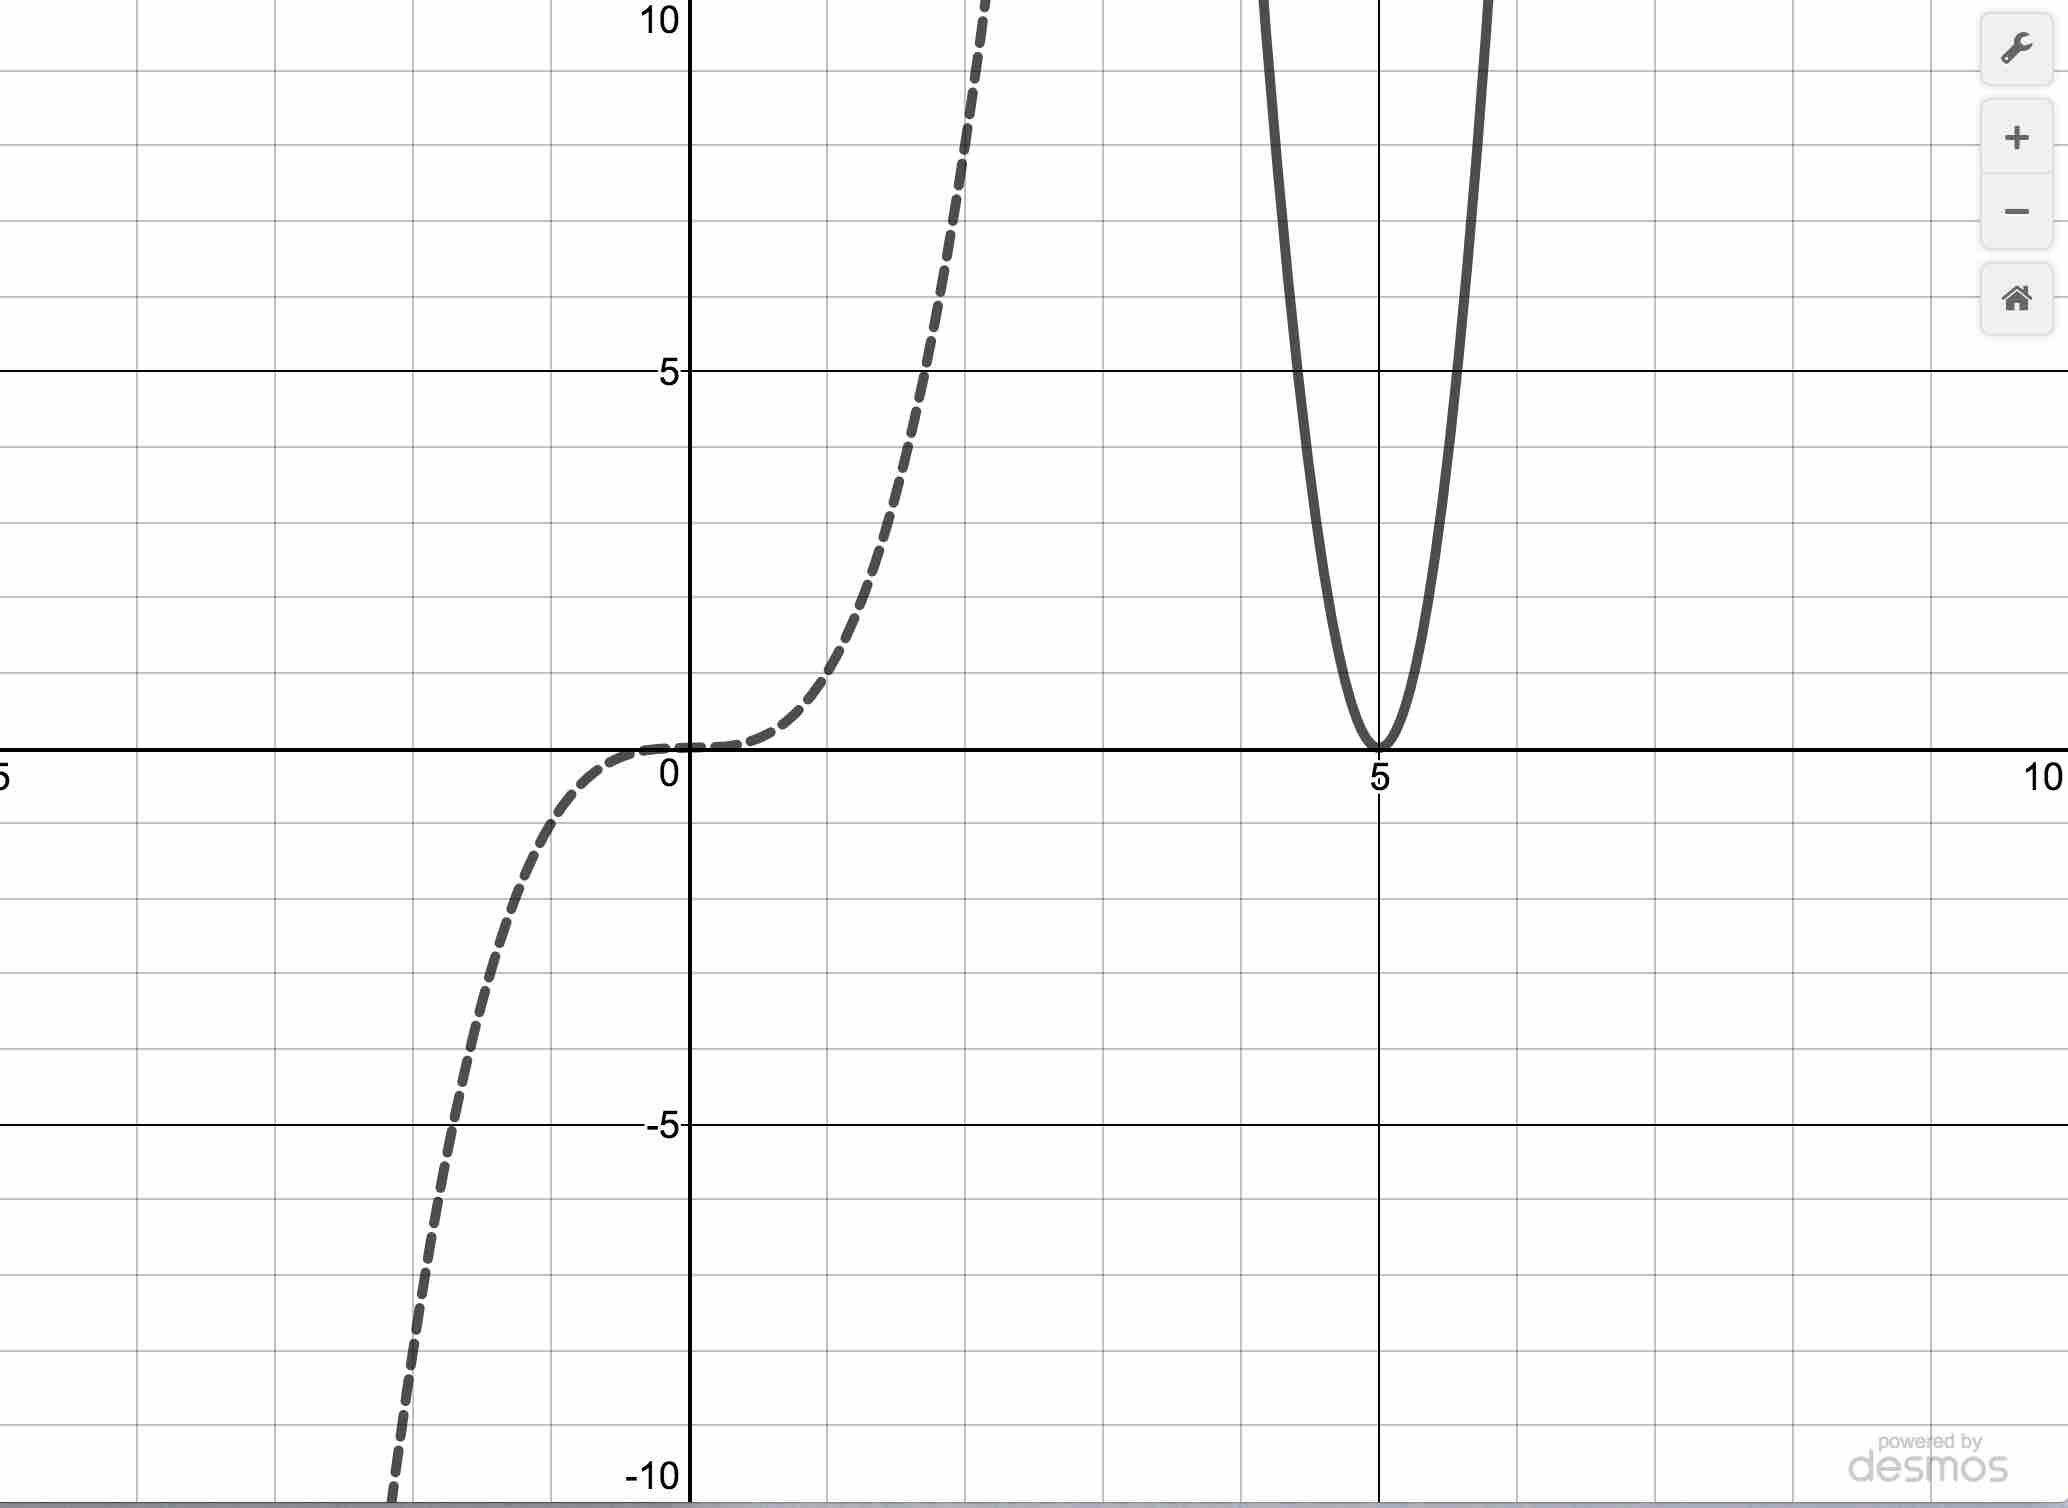
\includegraphics[height=2in]{./GraphsofPolynomialsGraphics/PolyEBEx1a.jpg}   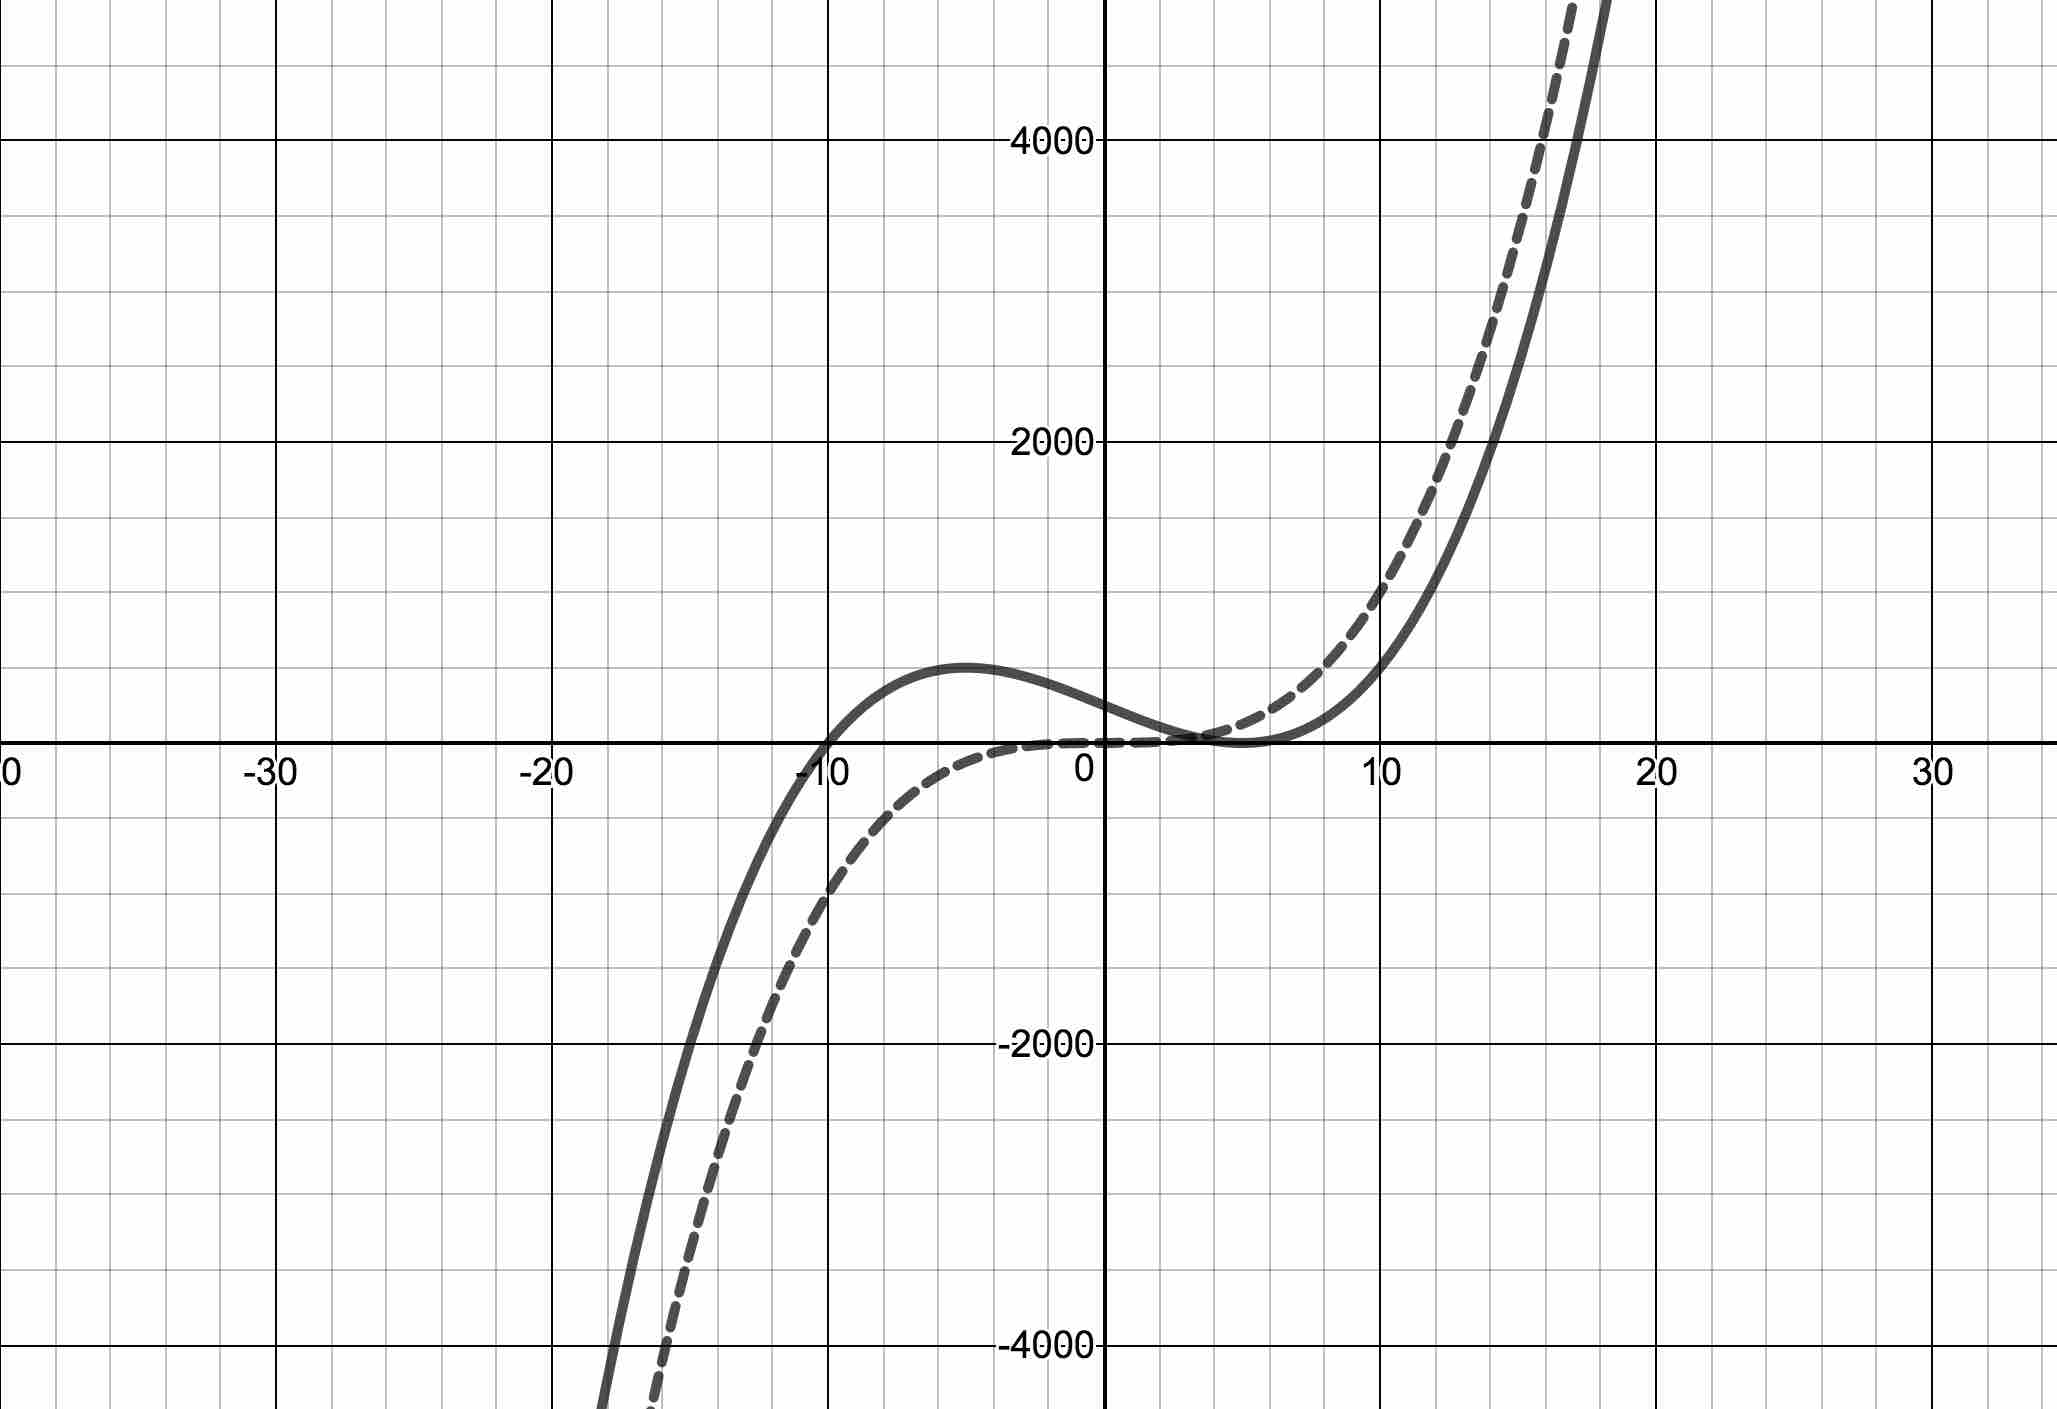
\includegraphics[height=2in]{./GraphsofPolynomialsGraphics/PolyEBEx1b.jpg} 


\end{multicols}


This observation is borne out numerically as well.  Based on the table below, as $x \rightarrow \pm \infty$, it certainly appears as if $f(x) \approx g(x)$.  One way to think about what is happening numerically is that the leading term $x^3$ \textit{dominates} the lower order terms  $-75x$ and $250$ as $x \rightarrow \pm \infty$.  In other words, $x^3$ grows so much faster than $-75 x$ and $250$ that these `lower order terms' don't contribute anything of significance to the $x^3$ so $f(x) \approx x^3$.  Another way to see this is to rewrite $f(x)$ as\footnote{Since we are considering  $x \rightarrow \pm \infty$, we are not concerned with $x$ even being close to $0$, so these fractions will all be defined.}   \[f(x) = x^3  - 75x + 250 = x^3 \left(1 -  \frac{75}{x^2} + \frac{250}{x^3} \right).\]   As $x \rightarrow \pm \infty$, both $\frac{75}{x^2}$ and $\frac{250}{x^3}$ have constant numerators but denominators that are becoming unbounded.  As such, both  $\frac{75}{x^2}$ and $\frac{250}{x^3} \rightarrow 0$.  Therefore, as $x \rightarrow \pm \infty$, \[ f(x) = x^3 - 75x+250  = x^3 \left(1 -  \frac{75}{x^2} + \frac{250}{x^3} \right) \approx x^3 (1 + 0 + 0) = x^3. \]

\[ \begin{array}{|r||c|c|c|c|c|c|}  \hline

 x &  f(x) = x^3 -75x+250 &  x^3 & -75 x & 250 & \frac{75}{x^2} &  \frac{250}{x^3}  \\ \hline
 -1000 & \approx -1 \times 10^9  &   -1 \times 10^9 &75000  & 250 & 7.5 \times 10^{-5} & -2.5 \times 10^{-7} \\  \hline
 -100 & \approx -9.9 \times 10^5 & -1 \times 10^6 & 7500  & 250 & 0.0075 & -2.5 \times 10^{-4} \\  \hline
 -10 & 0  & -1000  & 750 & 250  & 0.75   & -0.25\\  \hline
 10 & 500 &  1000 &  -750 & 250   & 0.75  &  0.25   \\ \hline
 100 &\approx 9.9 \times 10^5  & 1 \times 10^6 &   -7500  & 250 &  0.0075 &   2.5 \times 10^{-4} \\ \hline
 1000 & \approx 1 \times 10^9 & 1 \times 10^9  & -75000 & 250 & 7.5 \times 10^{-5} & 2.5 \times 10^{-7} \\  \hline

\end{array} \]


Next, consider  $g(x) = -0.01x^4 + 5x^2$.  Following the logic of the above example, we would expect the end behavior of $y=g(x)$ to mimic that of $y = -0.01 x^4$.  When we graph $y = g(x)$ (solid line) on the same set of axes as $y = -0.01x^4$ (dashed line), a view near the origin seems to suggest the exact opposite.  However, zooming out reveals that the two graphs do share the same end behavior.\footnote{Or at least they appear to within the limits of the technology.}


\begin{multicols}{2}

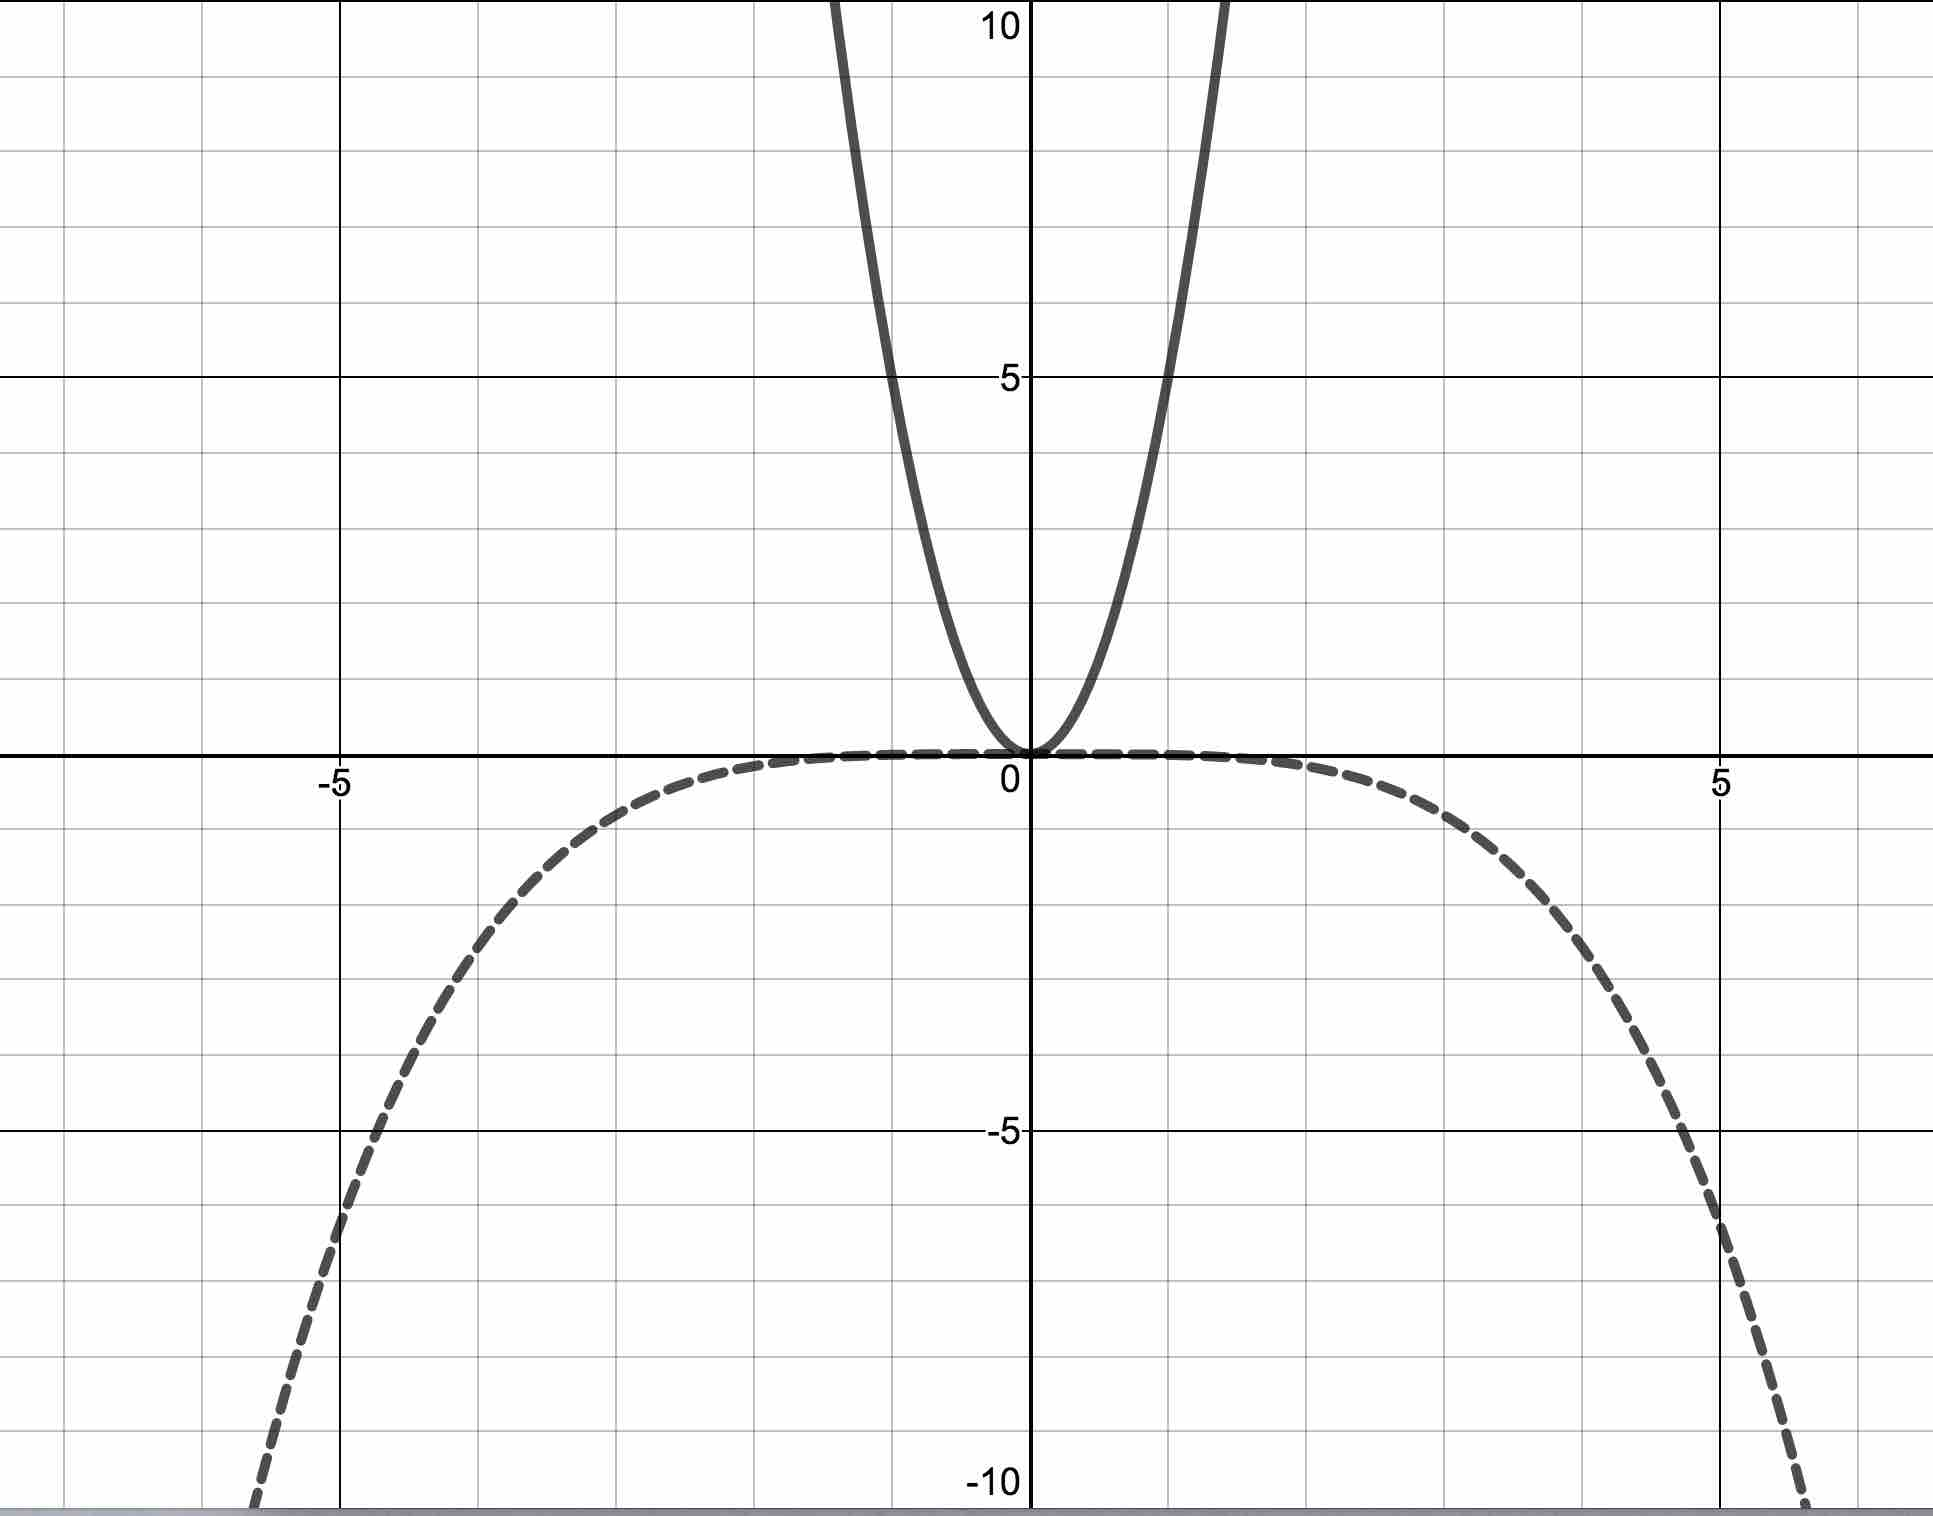
\includegraphics[height=2in]{./GraphsofPolynomialsGraphics/PolyEBEx2a.jpg}  \hspace{.5in} 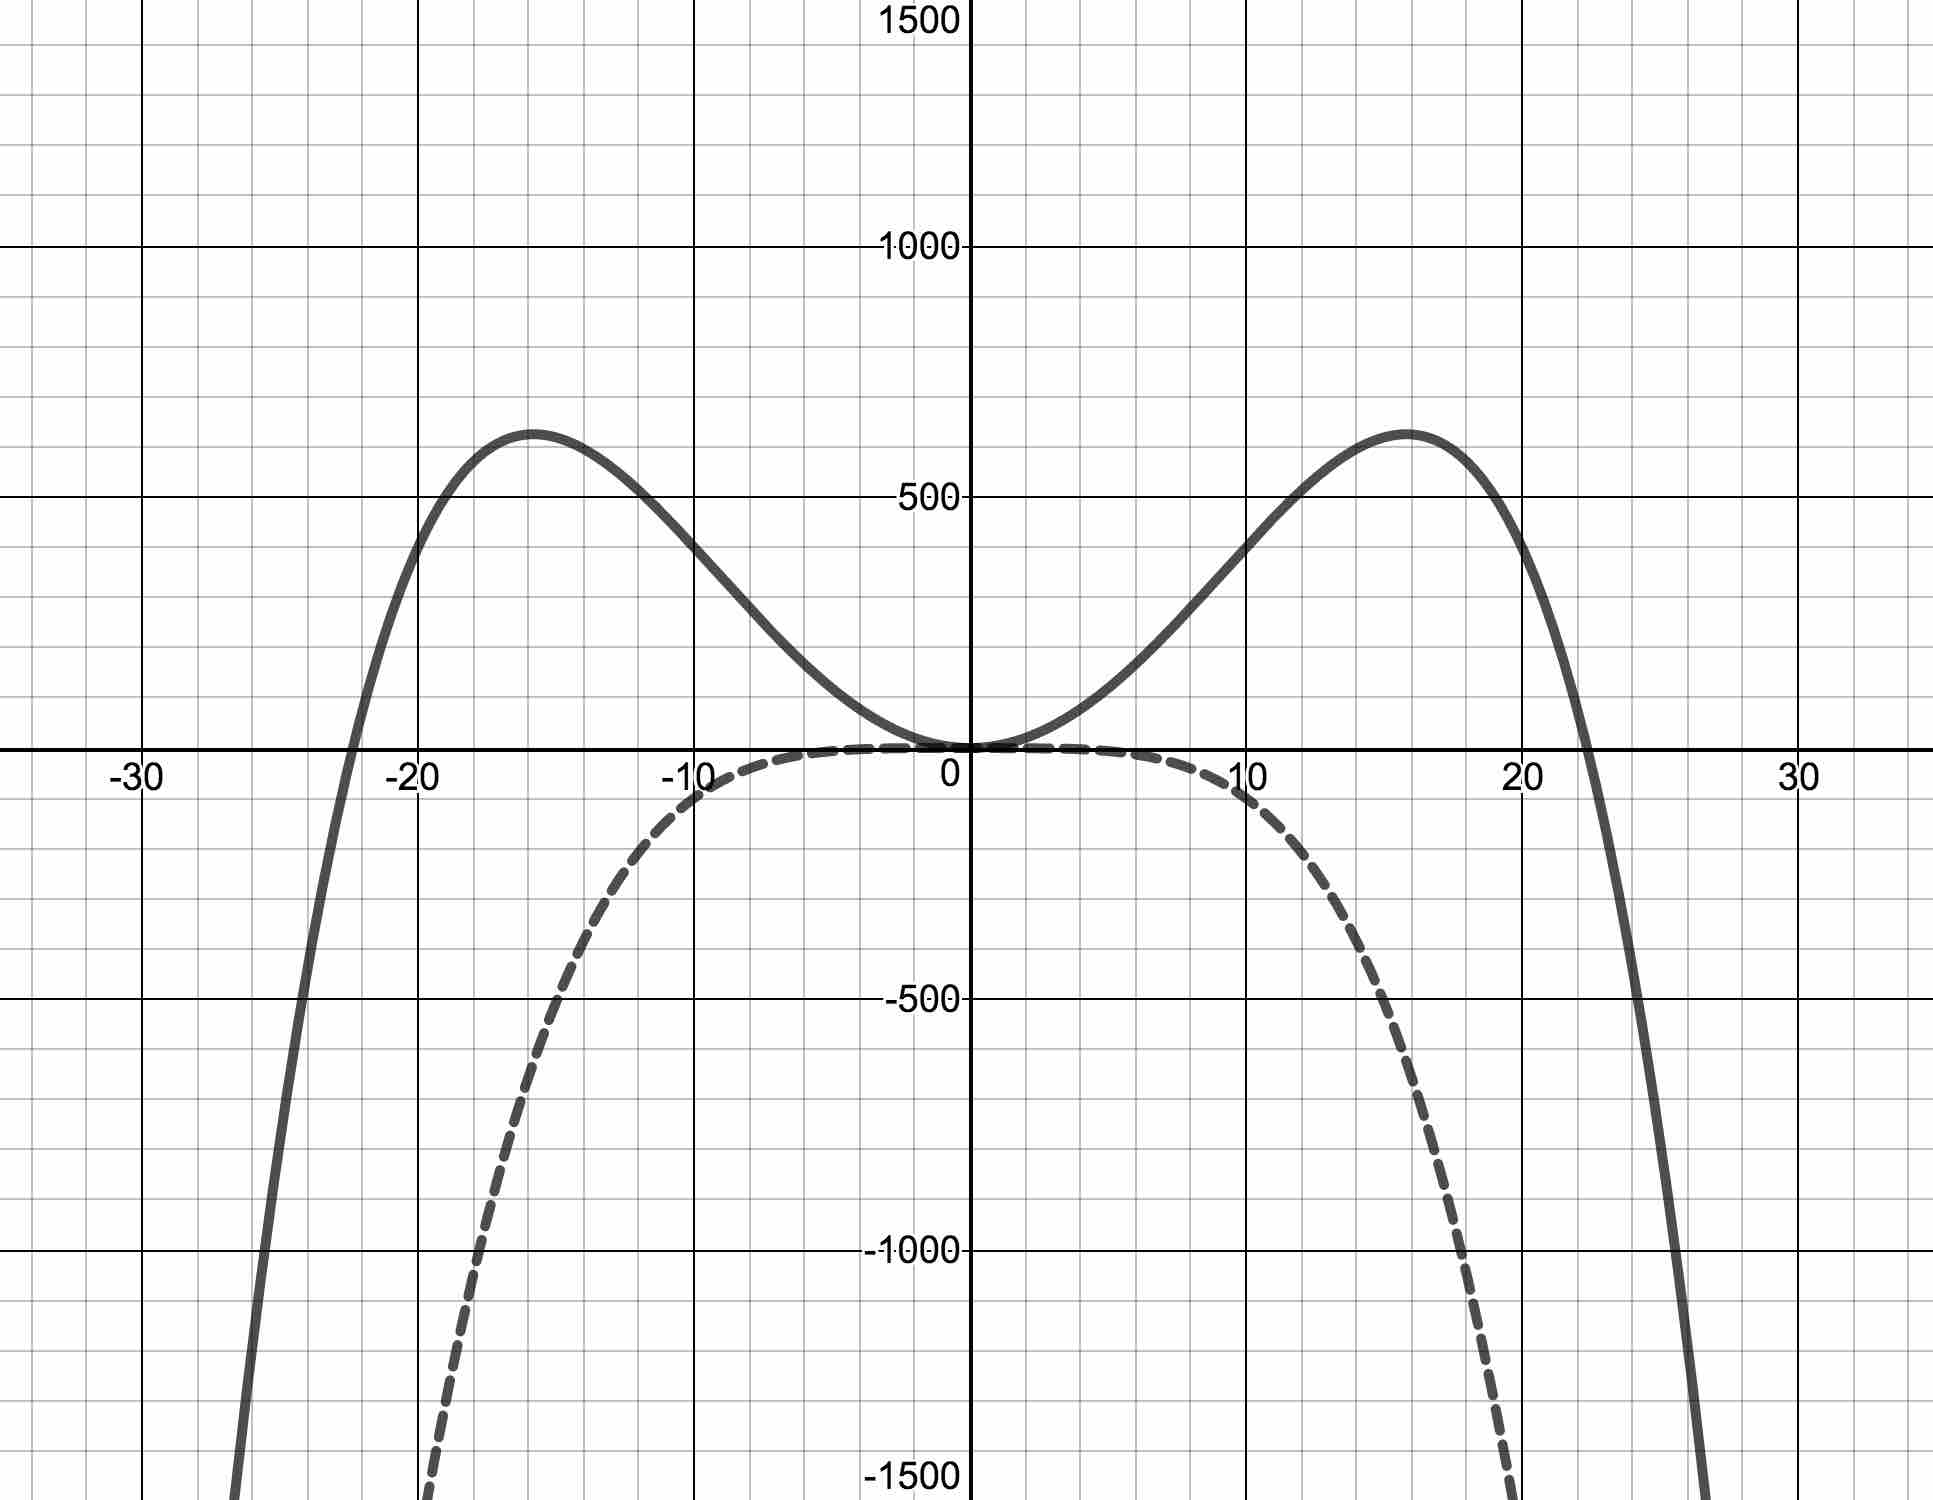
\includegraphics[height=2in]{./GraphsofPolynomialsGraphics/PolyEBEx2b.jpg} 


\end{multicols}

Algebraically, for $x \rightarrow \pm \infty$, even with the small coefficient of $-0.01$, $-0.01x^4$ dominates the $5x^2$ term so $g(x) \approx -0.01 x^4$.  More precisely, \[g(x) = -0.01x^4+5x^2 = x^4 \left(-0.01 + \frac{5}{x^2} \right) \approx x^4(-0.01 + 0)= -0.01x^4. \]

The results of these last two examples generalize below in Theorem \ref{EBPolynomials}.  


\colorbox{ResultColor}{\bbm

\begin{thm} \label{EBPolynomials}\index{end behavior ! polynomial}\textbf{End Behavior for Polynomial Functions:} 

The end behavior of  polynomial function $f(x) = a_{n} x^{n} + a_{n-\mbox{\tiny$1$}} x^{n-\mbox{\tiny$1$}} + \ldots + a_{\mbox{\tiny $2$}} x^{\mbox{\tiny $2$}} + a_{\mbox{\tiny $1$}} x + a_{\mbox{\tiny $0$}}$ with $a_{n} \neq 0$ matches the end behavior of $y = a_{n} x^{n}$.  

That is, the end behavior of a polynomial function is determined by its leading term.
\end{thm}

\ebm}

\medskip


We argue Theorem \ref{EBPolynomials} using an argument similar to ones used above.  As $x \rightarrow \pm \infty$, 

\[ f(x) =  x^{n} \left( a_{n} +\dfrac{a_{n-\mbox{\tiny$1$}}}{x}+ \ldots + \dfrac{a_{\mbox{\tiny$2$}}}{x^{n-2}} + \dfrac{a_{\mbox{\tiny$1$}}}{x^{n-1}}+\dfrac{a_{\mbox{\tiny$0$}}}{x^{n}}\right) \approx x^n( a_{n} + 0 +\ldots 0) = a_{n} x^n \]

If this argument looks a little fuzzy, it should.  In Calculus, we have the tools necessary to more explicitly state what we mean by $\approx 0$.  For now, we'll rely on number sense and algebraic intuition.\footnote{Both of which, by the way, can lead one astray, so we must proceed cautiously.}


Now that we know how to determine the end behavior of polynomial functions,  it's time to investigate what happens `in between' the ends.  First and foremost, polynomial functions are  \index{continuous}\index{function ! continuous}\textbf{continuous}.  Recall from Section \ref{QuadraticFunctions} that, informally, graphs of continuous functions have no `breaks' or `holes' in them.\footnote{Again, the formal definition of `continuity' and properties of continuous functions are discussed in Calculus.}   Since monomial functions are continuous (as far as we can tell) and polynomials are sums of monomial functions, it turns out that polynomial functions are continuous as well.   Moreover, the graphs of monomial functions, hence polynomial functions, are  \index{smooth}\index{function ! smooth}\textbf{smooth}.  Once again, `smoothness' is a concept defined precisely in Calculus, but for us,  functions have no `corners' or `sharp turns'.  Below we find the graph of a function which is neither smooth nor continuous, and to its right we have a graph of a polynomial, for comparison.  The function whose graph appears on the left fails to be continuous where it has a `break' or `hole' in the graph;  everywhere else, the function is continuous.  The function is continuous at the `corner' and the `cusp', but we consider these `sharp turns', so these are places where the function fails to be smooth.  Apart from these four places, the function is smooth and continuous.  Polynomial functions are smooth and continuous everywhere, as exhibited in the graph on the right.   The notion of smoothness is what tells us graphically that, for example, $f(x) = |x|$, whose graph is the characteristic `$\vee$' shape, cannot be a polynomial function, even though it is a piecewise-defined function comprised of polynomial functions.   Knowing polynomial functions are continuous and smooth gives us an idea of how to `connect the dots' when sketching the graph from points that we're able to find analytically such as intercepts.

\phantomsection
\label{cusppicture} 

\medskip

\begin{center}


\begin{tabular}{cc}

\begin{mfpic}[15]{-5}{5}{-2}{5}
\penwd{1.25pt}
\arrow \polyline{(-3,2),(-5,4)}
\arrow \function{-3,-1.5,0.1}{1-(2/(x+1))}
\dashed \polyline{(-1,0),(-1,5)}
\arrow \parafcn{-1,1.75,0.1}{(t**3,(t**2)+1)} 
\point[4pt]{(-1,2)}
\pointfillfalse
\point[4pt]{(3.375,3.25)}
\tlabel[cc](-3,1.5){\scriptsize  `corner'}
\tlabel[cc](-1,-0.5){\scriptsize `break'}
\tlabel[cc](0,0.5){\scriptsize `cusp'}
\tlabel[cc](3.375,2.5){\scriptsize `hole'}
\tcaption{\scriptsize Pathologies not found on graphs of polynomials functions.}
\end{mfpic}

\hspace{0.75in} &

\begin{mfpic}[15][7.5]{-5}{5}{-10}{10}
\penwd{1.25pt}
\arrow \reverse \arrow \function{-3,3.5,0.1}{0.5*x*(x+2)*(x-3)}
\tcaption{\scriptsize   The graph of a polynomial function.}
\end{mfpic}

\end{tabular}

\end{center}



Speaking of intercepts,  we next focus our attention on the behavior of the graphs of polynomial functions near their zeros.    Recall a zero $c$ of a function $f$ is a solution to $f(x) = 0$.  Geometrically, the zeros of a function are the $x$-coordinates of the $x$-intercepts of the graph of $y = f(x)$.    Consider the polynomial function $f(x) = x^3 (x-2)^2 (x+1)$. To find the zeros of $f$, we set $f(x) =  x^3 (x-2)^2 (x+1) = 0$.  Since the expression $f(x)$ is already factored, we set each factor equal to zero.\footnote{in accordance with the Zero Product Property of the Real Numbers - see Section \ref{AppRealNumberArithmetic}.}  Solving $x^3 = 0$ gives $x = 0$, $(x-2)^2 = 0$ gives $x = 2$, and $x+1 = 0$ gives $x = -1$.  Hence, our zeros are $x = -1$, $x = 0$, and $x = 2$.  Below, we graph $y = f(x)$ and observe the $x$-intercepts $(-1,0)$, $(0,0)$ and $(2,0)$.  We first note that the graph \textit{crosses} through the $x$-axis at $(-1,0)$ and $(0,0)$, but the graph \textit{touches} and \textit{rebounds} at $(2,0)$.  Moreover, at $(-1,0)$, the graph crosses through the axis is a fairly `linear' fashion whereas there is a substantial amount of `flattening' going on near $(0,0)$.  Or aim is to explain these observations and generalize them.

\begin{center}

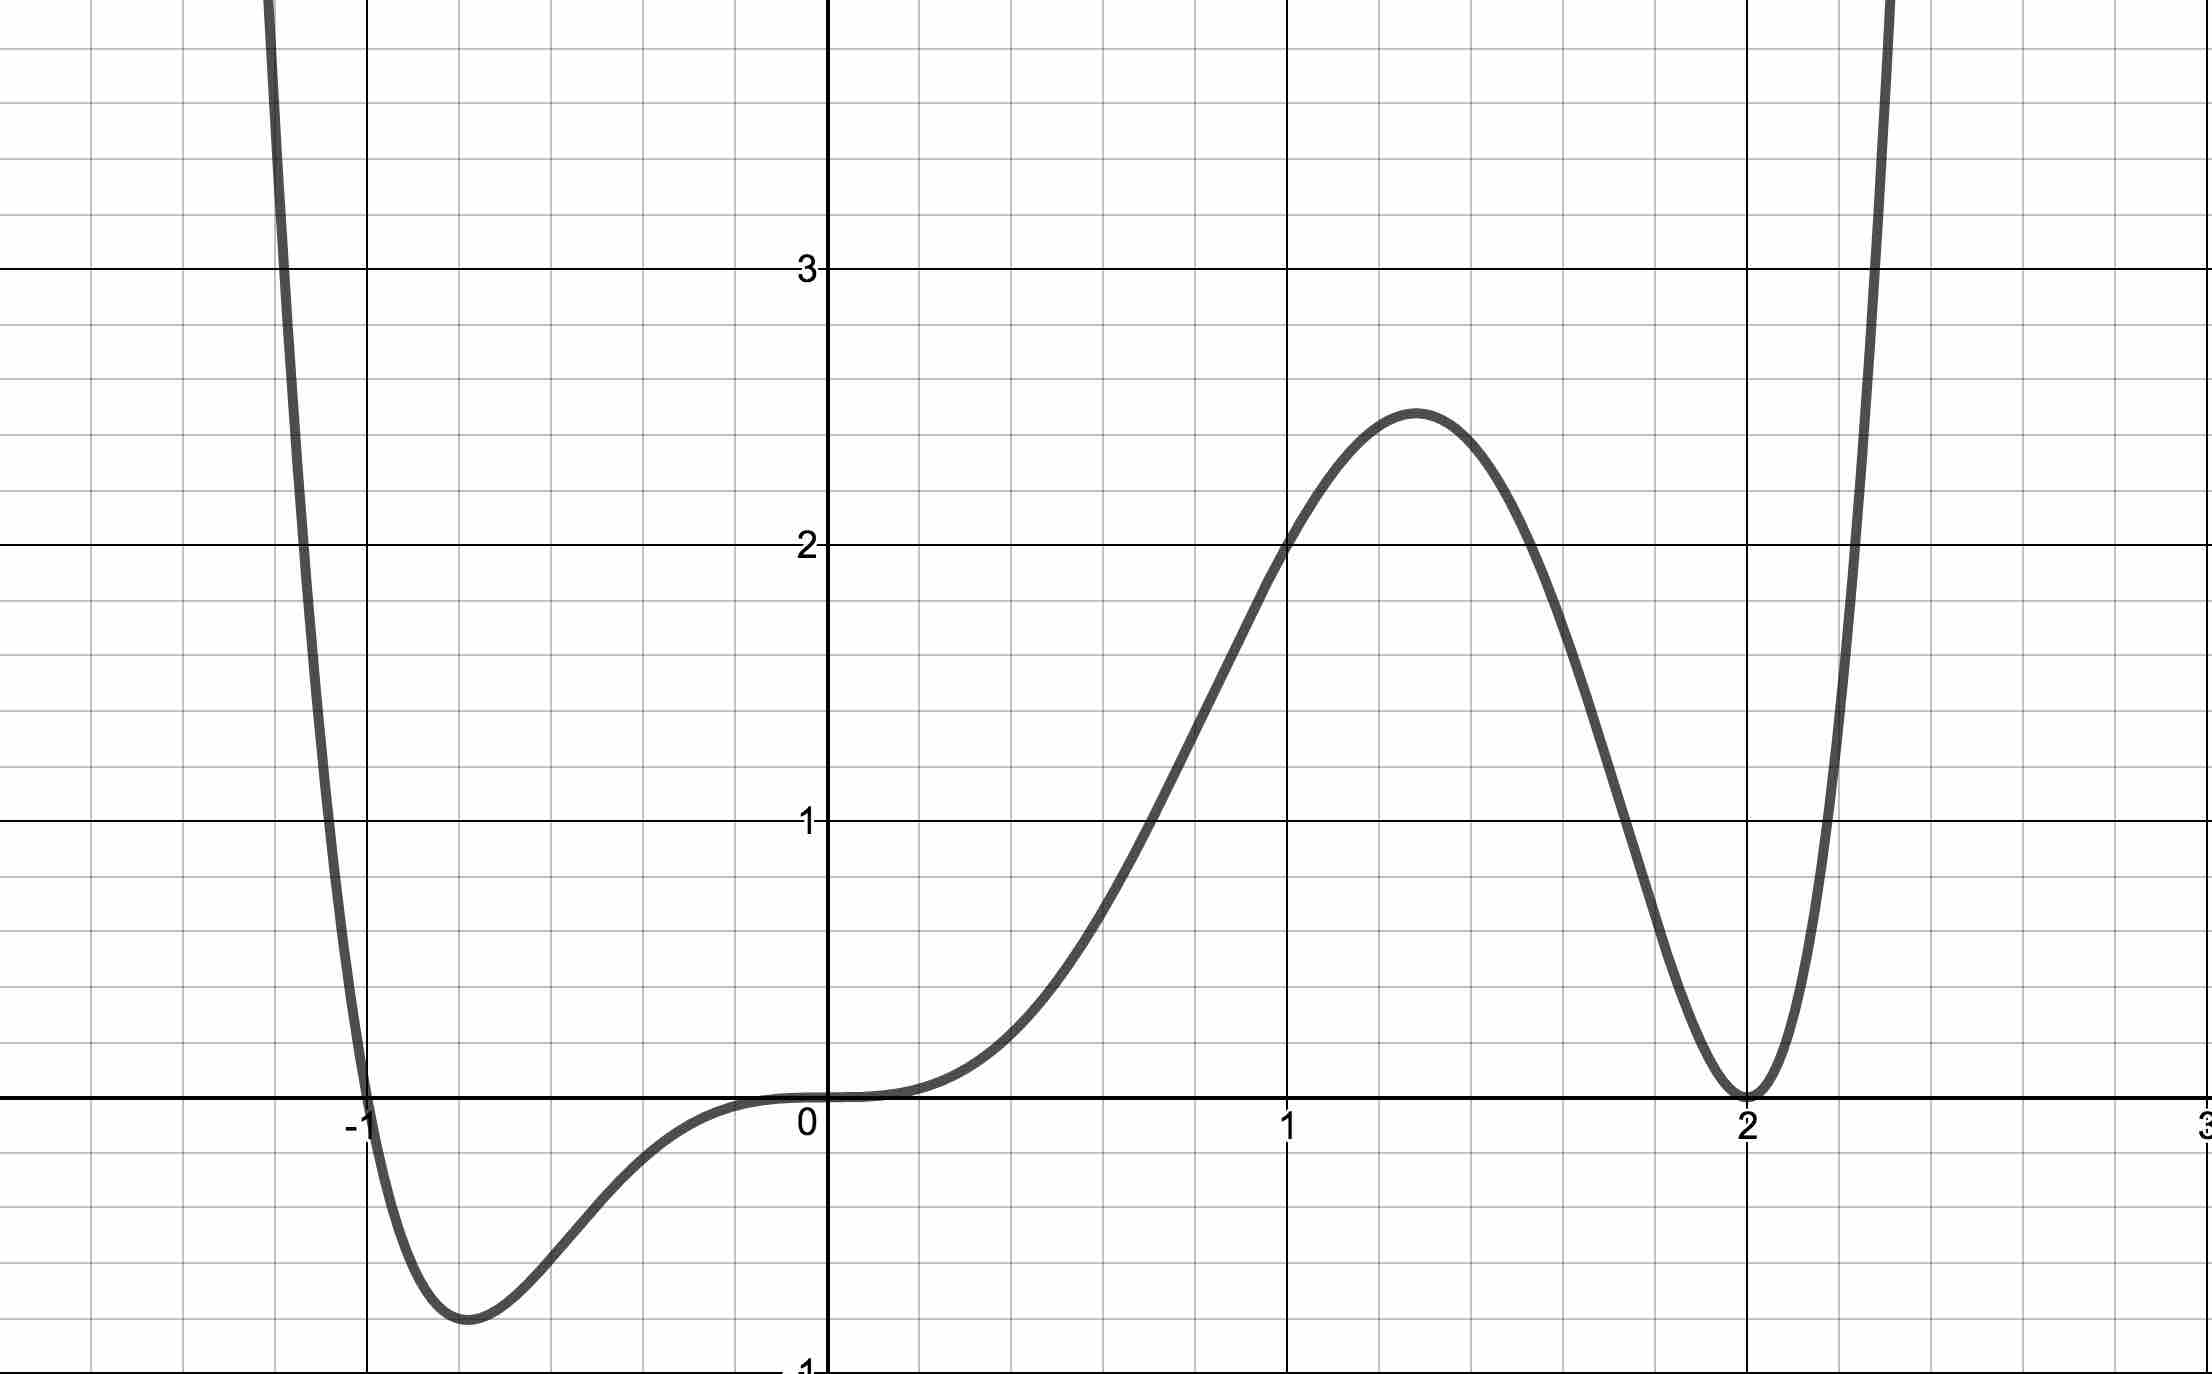
\includegraphics[height=3in]{./GraphsofPolynomialsGraphics/PolyZeroEx01.jpg} 

\end{center}

First, let's look at what's happening with the formula  $f(x) =  x^3 (x-2)^2 (x+1)$  when  $x  \approx  -1$.   We know the $x$-intercept at $(-1,0)$ is due to the presence of the $(x+1)$ factor in the expression for $f(x)$.  So, in this sense, the factor $(x+1)$ is determining a major piece of the behavior of the graph near $x = -1$.   For that reason, we focus instead on the other two factors to see what contribution they make. We find when $x \approx -1$,  $x^3  \approx  (-1)^3 = -1$ and $(x-2)^2 \approx (-1-2)^2 = 9$.  Hence, $f(x) = x^3 (x-3)^2 (x+1) \approx (-1)^3 (-1-2)^2 (x+1) = -9(x+1)$.  Below on the left is a graph of $y = f(x)$ (the solid line) and the graph of $y = -9(x+1)$ (the dashed line.)  Sure enough, these graphs approximate one another near $x = -1$. 

Likewise, let's look near $x = 0$.  The $x$-intercept $(0,0)$ is due to the $x^3$ term.  For $x \approx 0$, $(x-2)^2 \approx (0-2)^2 = 4$ and $(x+1) \approx (0+1) = 1$, so $f(x) =  x^3 (x-3)^2 (x+1) \approx x^3 (-2)^2(1) = 4x^3$.  Below in the center picture, we have the graph of $y = f(x)$ (again, the solid line) and $y = 4x^3$ (the dashed line) near $x=0$.  Once again, the graphs verify our analysis.

Last, but not least, we analyze $f$ near $x = 2$.  Here, the intercept $(2,0)$ is due to the $(x-2)^2$ factor, so we look at the $x^3$ and $(x+1)$ factors.  If $x \approx 2$, $x^3 \approx (2)^3 = 8$ and $(x+1) \approx (2+1) = 3$.  Hence,  $f(x) =  x^3 (x-3)^2 (x+1) \approx (2)^3 (x-2)^2 (2+1) = 24(x-2)^2$.  Sure enough, as evidenced below on the right, the graphs of $y = f(x)$ and $y = 24(x-2)^2$.


\begin{tabular}{m{2in}m{2in}m{2in}}

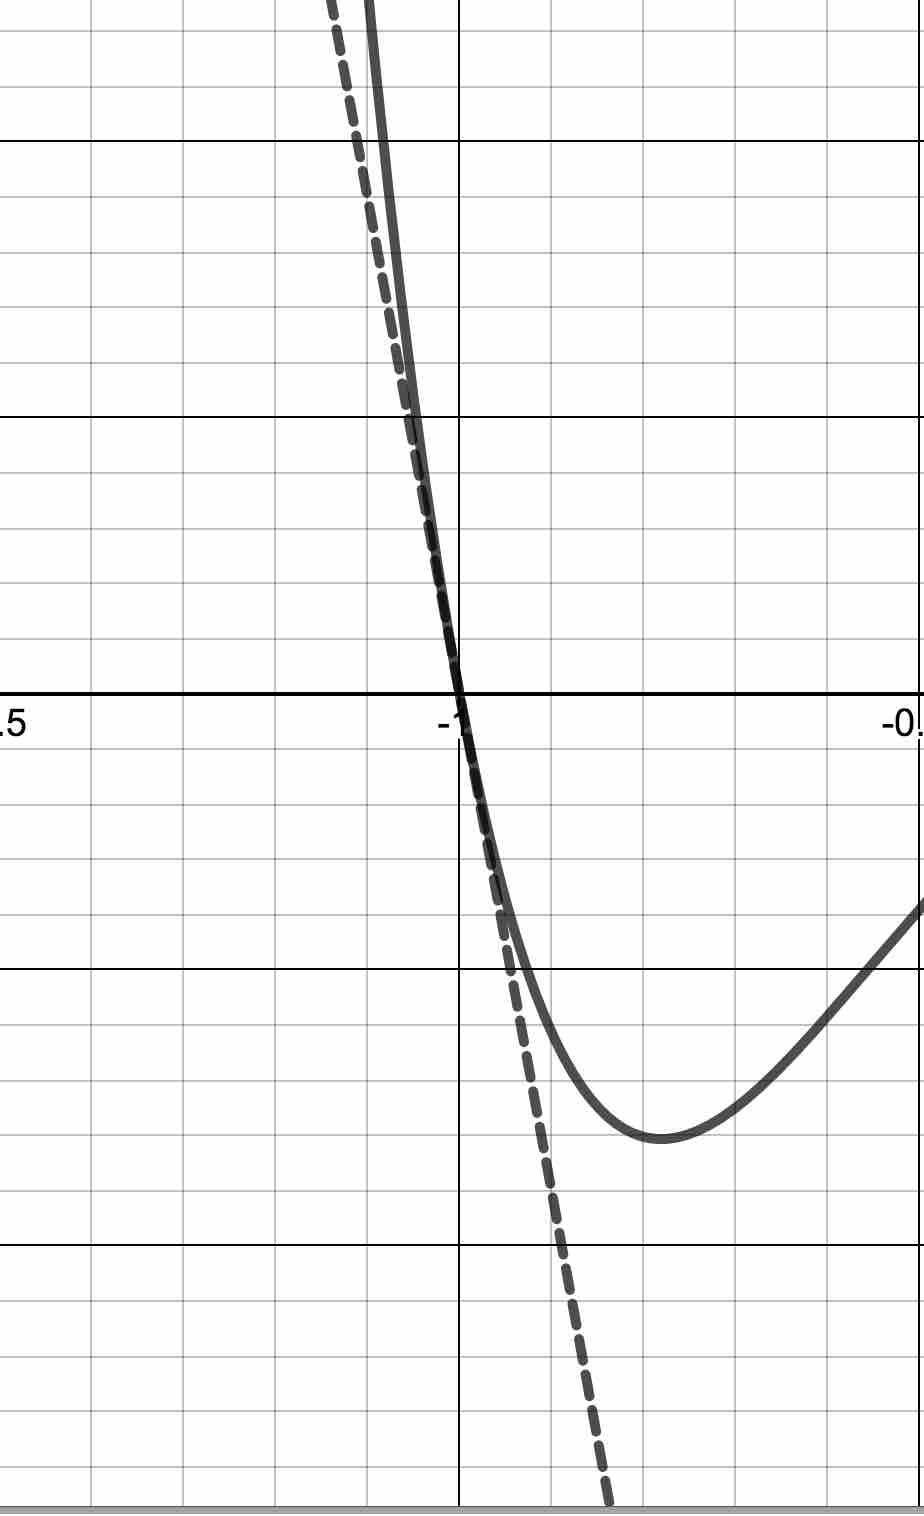
\includegraphics[height=2.in, width=2.in]{./GraphsofPolynomialsGraphics/PolyZeroEx02.jpg} 
&

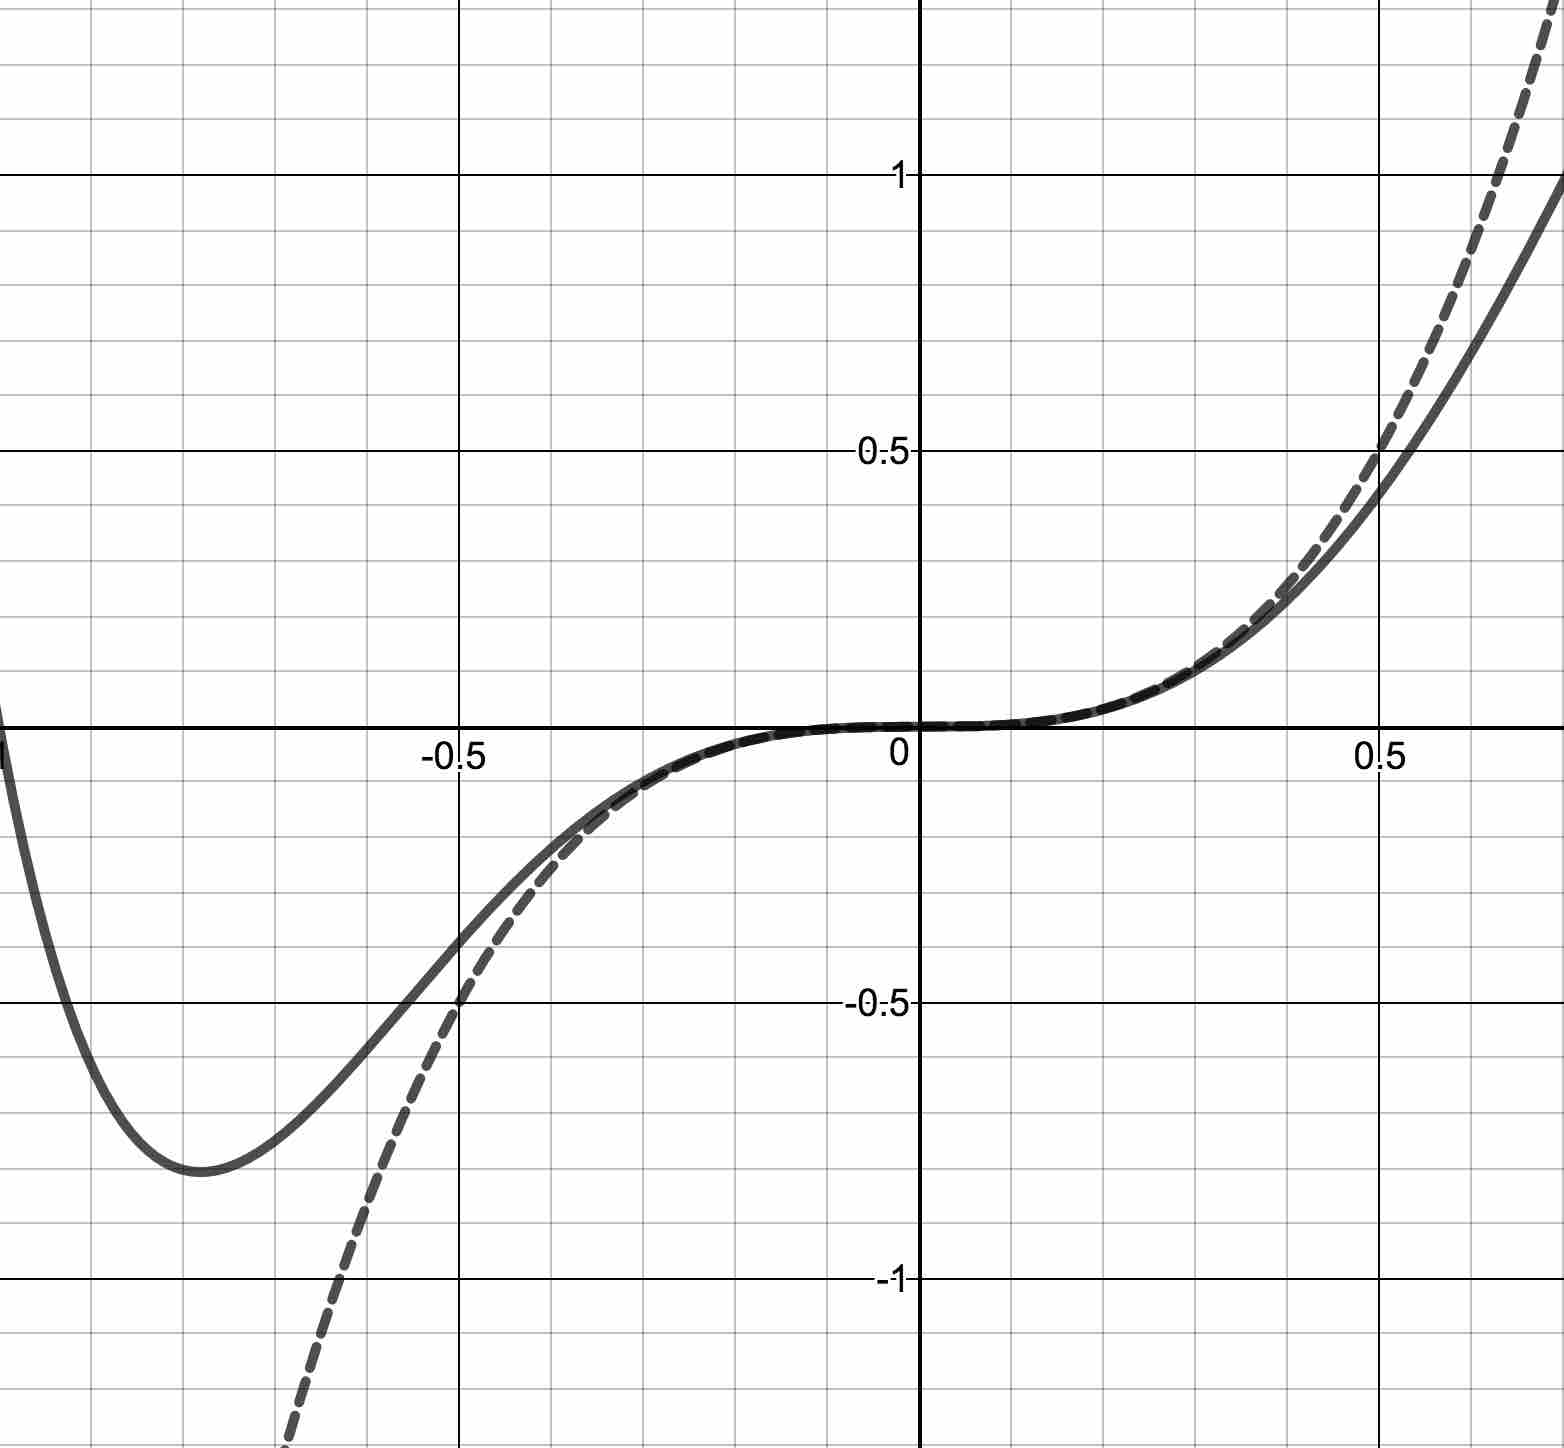
\includegraphics[height=2.in, width=2.in]{./GraphsofPolynomialsGraphics/PolyZeroEx03.jpg} 

&

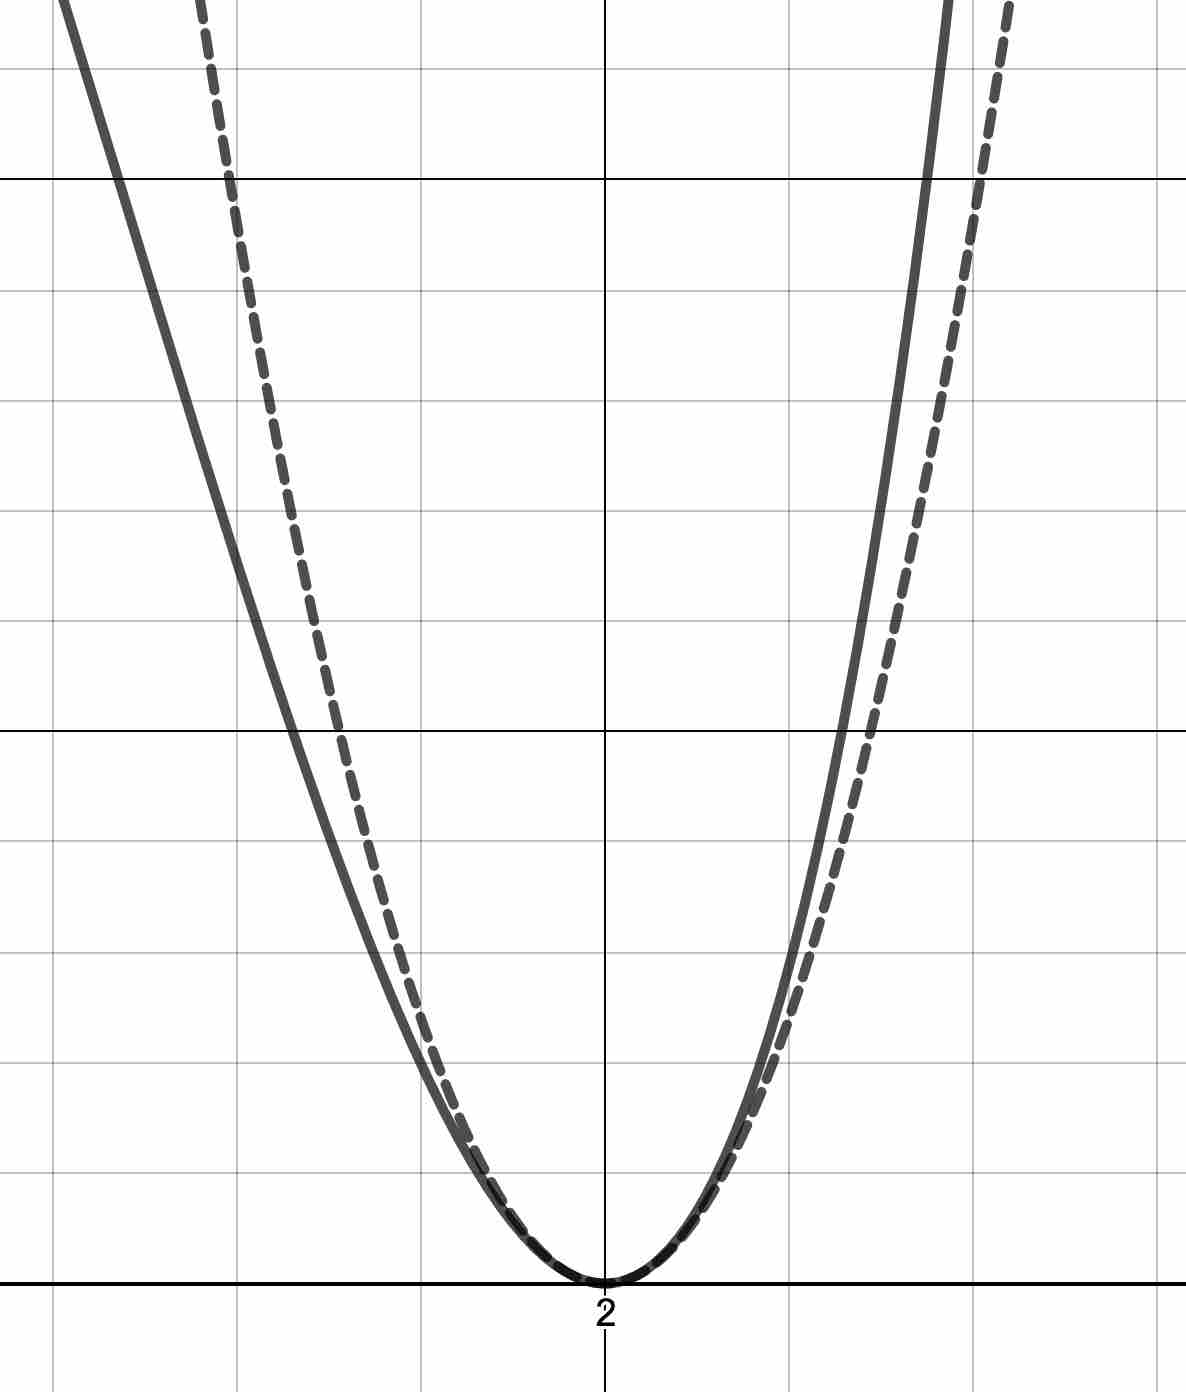
\includegraphics[height=2.in, width=2.in]{./GraphsofPolynomialsGraphics/PolyZeroEx04.jpg}  \\

$y = f(x)$ and $y = -9(x+1)$

&

$y = f(x)$ and $y = 4x^3$ 

&

$y = f(x)$ and $y=24(x-2)^2$ \\

\end{tabular}

We generalize our observations in Theorem \ref{polynomialbehaviornearzeros} below. Like many things we've seen in this text, a more precise statement and proof can be found in a course on Calculus.

\colorbox{ResultColor}{\bbm

\begin{thm}  \label{polynomialbehaviornearzeros}  Suppose $f$ is a polynomial function and $f(x) = (x-c)^m q(x)$ where $m \in \mathbb{N}$ and $q(c) \neq 0$.  Then the the graph of $y = f(x)$ near $(c,0)$ resembles that of $y = q(c) (x-c)^m$.


\end{thm}

\ebm}

Let's see how Theorem \ref{polynomialbehaviornearzeros}  applies to our findings regarding $f(x) =  x^3 (x-2)^2 (x+1)$. For $c = -1$, $(x-c) = (x-(-1)) = (x+1)$.  We  rewrite $f(x) =  x^3 (x-2)^2 (x+1) = (x-(-1))^1 \left[x^3(x-2)^2\right]$ and identify $m=1$ and $q(x) = x^3 (x-2)^2$.  We find $q(c) = q(-1) = (-1)^3(-1-2)^2 = -9$ so  Theorem \ref{polynomialbehaviornearzeros} says that near $(-1,0)$, the graph of $y=f(x)$ resembles $y = q(-1)(x-(-1))^1 = -9(x+1)$.  For $c=0$, $(x-c) = (x-0) = x$ and we can rewrite $f(x) =  x^3 (x-2)^2 (x+1) = (x-0)^3 \left[(x-2)^2 (x+1)\right]$.  We identify $m=3$ and $q(x) = (x-2)^2(x+1)$.  In this case $q(c) = q(0) = (0-2)^2(0+1) = 4$, so  Theorem \ref{polynomialbehaviornearzeros} guarantees the graph  of $y = f(x)$ near $x=0$ resembles  $y = q(0)(x-0)^3 = 4x^3$.  Lastly, for $c = 2$, we see $f(x) = (x-2)^2 \left[x^3 (x+1)\right]$ and we identify $m = 2$ and $q(x) = x^3(x+1)$.  We find $q(2) = 2^3 (2+1)= 24$, so  Theorem \ref{polynomialbehaviornearzeros}  guarantees the graph of $y = f(x)$ resembles $y = 24(x-2)^2$ near $x=2$.

As we already mentioned,  the formal statement and proof of Theorem \ref{polynomialbehaviornearzeros} require Calculus.  For now, we can understand the theorem as follows.   If we factor a polynomial function as $f(x) = (x-c)^m q(x)$ where $m \geq 1$,   then $x=c$ is a zero of $f$, since $f(c) = (c-c)^m q(c) = 0 \cdot q(c) = 0$.  The stipulation that $q(c) \neq 0$ means that we have essentially factored the expression $f(x) = (x-c)^m q(x) = (\text{going to $0$}) \cdot (\text{not going to $0$})$.   Thinking back to Theorem \ref{linearmononialgraphs}, the graph $y = q(c) (x-c)^m$ has an $x$-intercept at $(c,0)$, a basic overall shape determined by the exponent $m$, and end behavior determined by the sign of $q(c)$.   The fact that \textit{if} $x=c$ is a zero \textit{then} we are guaranteed we can factor $f(x) = (x-c)^m q(x)$ were $q(c) \neq 0$ and, moreover, such a factorization is unique (so that there's only one value of $m$ possible for each zero) is a consequence of two theorems, Theorem \ref{polydivthm} and The Factor Theorem, Theorem \ref{factorthm} which we'll review in Section \ref{Polydivision}.  For now, we assume such a factorization is unique in order to define the following.

\colorbox{ResultColor}{\bbm

\begin{defn} \label{multiplicity} Suppose $f$ is a polynomial function and $m \in \mathbb{N}$. If $f(x) = (x-c)^m q(x)$ where $q(c) \neq 0$, we say  $x=c$ is a zero of \index{polynomial function ! zero ! multiplicity}\index{multiplicity ! of a zero}\index{zero ! multiplicity of}\textbf{multiplicity} $m$.

\end{defn}

\ebm}

So, for $f(x) =  x^3 (x-2)^2 (x+1) = (x-0)^3(x-2)^2(x-(-1))^1$, $x=0$ is a zero of multiplicity $3$, $x=2$ is a zero of multiplicity $2$, and $x =-1$ is a zero of multiplicity $1$.  Theorems   \ref{EBPolynomials}  and \ref{polynomialbehaviornearzeros} give us the following:


\colorbox{ResultColor}{\bbm

\begin{thm} \label{roleofmultiplicity} \textbf{The Role of Multiplicity:}  Suppose $f$ is a polynomial function  and $x=c$ is a zero of multiplicity $m$.  \index{multiplicity ! effect on the graph of a polynomial}

\begin{itemize}

\item  If $m$ is even, the graph of $y=f(x)$ touches and rebounds from the $x$-axis at $(c,0)$.

\item  If $m$ is odd, the graph of $y=f(x)$ crosses through the $x$-axis at $(c,0)$.

\end{itemize}

\end{thm}

\ebm}


Our next example showcases how all of the above theory can assist in sketching relatively good graphs of polynomial functions without the assistance of technology.

\begin{ex} \label{graphfromtheory}   Let $p(x) = (2x-1)(x+1)(1-x^4)$.

\begin{enumerate}

\item Find all real zeros of $p$ and state their multiplicities.

\item  Describe the behavior of the graph of $y = p(x)$ near each of the $x$-intercepts.

\item  Determine the end behavior  and $y$-intercept of the graph of  $y = p(x)$.

\item  Sketch $y = p(x)$ and check your answer using a graphing utility.

\end{enumerate}

{\bf Solution.}

\begin{enumerate}

\item  To find the zeros of $p$, we set  $p(x) =  (2x-1)(x+1)(1-x^4) = 0$.  Since the expression $p(x)$ is already (partially) factored, we set each factor equal to $0$ and solve.  From $(2x-1) =0$, we get $x=\frac{1}{2}$; from $(x+1) = 0$ we get  $x = -1$; and from  solving $1-x^4 =0$ we get $x = \pm 1$.  Hence, the zeros are $x = -1$, $x = \frac{1}{2}$, and $x = 1$.  In order to determine the multiplicities, we need to factor $p(x)$ as so we can identify the $m$ and $q(x)$ as described in Definition \ref{multiplicity}.  The zero $x = -1$ corresponds to the factor $(x+1)$.  Notice, however, that writing $p(x) = (x+1)^1 \left[(2x-1)(1-x^4)\right]$ with $m = 1$ and $q(x) = (2x-1)(1-x^4)$ does \textit{not} satisfy Definition \ref{multiplicity} since here, $q(-1) = (2(-1)-1)(1-(-1)^4) = 0$.  Indeed, we can factor $(1-x^4) = (1-x^2)(1+x^2) = (1-x)(1+x)(x^2+1)$ so that \[p(x)= (2x-1)(x+1)(1-x^4)  = (2x-1)(x+1)(1-x)(1+x)(x^2+1) = (x+1)^2 \left[(2x-1)(1-x)(x^2+1) \right].\]
Identifying $q(x) = (2x-1)(1-x)(x^2+1)$, we find $q(-1) = (2(-1)-1)(1-(-1))((-1)^2+1) = -12 \neq 0$, which means the multiplicity of $x=-1$ is $m=2$.  

The zero $x = \frac{1}{2}$ came from the factor $(2x-1) = 2 (x-\frac{1}{2})$, so we have \[ p(x) =  (2x-1)(x+1)^2(1-x)(x^2+1)  = (x -\frac{1}{2})^{1} \left[2 (x+1)^2(1-x)(x^2+1) \right]. \] If we identify $q(x) = 2 (x+1)^2(1-x)(x^2+1)$, we find $q(\frac{1}{2}) = \frac{45}{16} \neq 0$ so multiplicity here is $m=1$.  

Last but not least, we turn our attention to our last zero, $x = 1$, which we obtained from solving $1-x^4=0$.  However, from $p(x) =  (2x-1)(x+1)^2(1-x)(x^2+1)$, we see the zero $x=1$ corresponds to the factor $(1-x) = -(x-1)$.  We have $p(x) = (x-1)^{1}\left[- (2x-1)(x+1)^2(x^2+1)\right]$.  Identifying $q(x) = - (2x-1)(x+1)^2(x^2+1)$, we see $q(1) = -8$, so the multiplicity $m = 1$ here as well.  


\item  From Theorem \ref{roleofmultiplicity}, since the multiplicities of $x = \frac{1}{2}$ and $x = 1$ are both \textit{odd}, we know the graph of $y = p(x)$ \textit{crosses} through the $x$-axis at $(\frac{1}{2}, 0)$ and $(1,0)$. More specifically, since the multiplicity for both of these zeros is $1$,  the graph will look locally linear at these points. More specifically, based on our calculations above, near $x = \frac{1}{2}$, the graph will resemble the increasing line $y =  \frac{45}{16} (x - \frac{1}{2})$, and near  $x = 1$, the graph will resemble the decreasing line $y = -8(x-1)$.    Since the multiplicity of $x = -1$ is \textit{even}, we know the graph of $y = p(x)$ \textit{touches} and  \textit{rebounds} at $(-1,0)$.   Since the multiplicity of $x=-1$ is $2$, it will look locally like a parabola.   More specifically, the graph near $x = -1$ will resemble $y = -12(x+1)^2$.

\item  Per Theorem \ref{EBPolynomials}, the end behavior of $y =p(x)$, matches the end behavior of its leading term.  As in Example \ref{degreandallthatexample}, we multiply the leading terms from each factor together to obtain the leading term for $p(x)$ :   $p(x) = (2x-1)(x+1)(1-x^4) = (2x)(x)(-x^4) + \ldots = -2x^6 + \ldots$.  Since the degree here, $6$, is even and the leading coefficient $-2 <0$, we know as $x \rightarrow \pm \infty$, $p(x) \rightarrow -\infty$.  To find the $y$-intercept, we find $p(0) = (2(0)-1)(0+1)(1-0^4) = -1$, hence, the $y$-intercept is $(0,-1)$.  

\item  From the end behavior, $x \rightarrow -\infty$, $p(x) \rightarrow -\infty$, we start the graph in Quadrant III and head towards $(-1,0)$. At $(-1,0)$, we `bounce' off of the $x$-axis and head towards the $y$-intercept, $(0,-1)$.  We then head towards $\left(\frac{1}{2}, 0 \right)$ and cross through the $x$-axis there.  Finally, we head back to the $x$-axis and cross through at $(1,0)$.  Owing to the end behavior $x \rightarrow \infty$, $p(x) \rightarrow -\infty$, we exit the picture in Quadrant IV.  Since polynomial functions are continuous and smooth, we have no holes or gaps in the graph, and all the `turns' are rounded (no abrupt turns or corners.)  We produce something resembling the graph below.

\begin{center}

\begin{mfpic}[40][20]{-2}{2}{-4}{2}
\axes
\scriptsize
\tlabel[cc](2, -0.5){$x$}
\tlabel[cc](0.25, 2){$y$}
\tlabel[cc](-1,0.5){$(-1,0)$}
\tlabel[cc](0.5,-1){$(0,-1)$}
\tlabel[cc](0.25, 0.5){$\left( \frac{1}{2},0 \right)$}
\tlabel[cc](1.25,0.5){$(1,0)$}
\normalsize
\penwd{1.25pt}
\arrow \reverse \arrow \function{-1.35,1.2,0.1}{(2*x-1)*(x+1)*(1-(x**4))}
\point[4pt]{(-1,0), (0.5,0), (1,0), (0,-1)}
\tcaption{\scriptsize $y=p(x)$}
\end{mfpic} 

\end{center}

\qed

\end{enumerate}


\end{ex}

A couple of remarks about Example \ref{graphfromtheory} are in order.  First, notice that the factor $(x^2+1)$ was more of a spectator in our discussion of the zeros of $p$. Indeed, if we set $x^2+1 = 0$, we have $x^2=-1$ which provides no \textit{real} solutions.\footnote{The solutions are $x = \pm i$ - see Section \ref{AppCmpNums}.}  That being said, the factor $x^2+1$ \textit{does} affect the shape of the graph (See Exercise \ref{comparegraphfromtheoryexample}.) Next, when connecting up the graph from $(-1,0)$ to $(0,-1)$ to $\left(\frac{1}{2}, 0 \right)$, there really is no way for us to know how low the graph goes, or where the lowest point is between $x = -1$ and $x = \frac{1}{2}$  unless we plot more points.  Likewise, we have no idea how high the graph gets between $x = \frac{1}{2}$ and $x = 1$.  While there are ways to determine these points analytically, more often than not, finding them requires Calculus.   Since these points do play an important role in many applications, we'll need to discuss them in this course and, when required, we'll  use technology to find them.   For that reason, we have the following definition:

\colorbox{ResultColor}{\bbm
\begin{defn}

\label{localmaxmindefn}

Suppose $f$ is a function with $f(a) = b$.

\begin{itemize}

\item  We say $f$ has a \textbf{local minimum} at the point $(a,b)$ if and only if there is an open interval $I$ containing $a$ for which $f(a) \leq f(x)$ for all $x$ in $I$.  The value $f(a) = b$ is called `a  local minimum value of $f$.' \index{local minimum ! formal definition of}

That is, $b$ is the minimum $f(x)$ value over an \textit{open interval}  containing $a$. 

 Graphically,  no points `near' a local minimum are lower than $(a,b)$. 

\item  We say $f$ has a \textbf{local maximum} at the point $(a,b)$ if and only if there is an open interval $I$ containing $a$ for which $f(a) \geq f(x)$ for all $x$ in $I$.  The value $f(a) = b$ is called `a  local maximum value of $f$.' \index{local maximum ! formal definition of}

That is, $b$ is the maximum $f(x)$ value over an \textit{open interval} containing $a$.  

Graphically, no points `near' a local maximum are higher than $(a,b)$. 

\end{itemize}

Taken together, the local maximums and local minimums of a function, if they exist,  are called the \textbf{local extrema} of the function. \index{local extrema ! formal definition of}



\end{defn}

\ebm}

Once again, the terminology used in Definition \ref{localmaxmindefn}  blurs the line between the function $f$ and its outputs, $f(x)$.  Also, some textbooks use the terms `relative' minimum and `relative' maximum instead of the adjective `local.'  Lastly, note  the definition of local extrema requires an \textit{open} interval exist in the domain containing $a$ in order for $(a, f(a))$ to be a candidate for a local maximum or local minimum. We'll have more to say about this in later chapters.  If our open interval happens to be $(-\infty, \infty)$, then our local extrema are the extrema of $f$ - we'll see an example of this momentarily.  

Below we use a graphing utility to graph $y= p(x) = (2x-1)(x+1)(1-x^4)$.    We first consider the point $(-1,0)$.   Even though there are points on the graph of $y = p(x)$ that are higher than $(-1,0)$,  locally, $(-1,0)$ is the top of a hill.  To satisfy Definition \ref{localmaxmindefn}, we need to provide an open interval on which $p(-1) = 0$ is the largest, or maximum function value. Note the definition requires us to provide \textit{just one} open interval.  One that works is the interval $(-1.5, -0.5)$.   We could use any smaller interval or go as large as $\left(-\infty, \frac{1}{2} \right)$ (can you see why?)  Next we encounter  a `low' point at approximately $(-0.2353, -1.1211)$. More specifically, for all $x$ in the interval, say,  $(-0.5, 0)$, $p(x) \geq 1.1211$,  Hence, we have a local minimum at $(-0.2353, -1.1211)$.   Lastly, at $(0.811, 0.639)$, we are back to a high point.  In fact, $0.639$ isn't just a local maximum value, based on the graph, it is \textit{the} maximum of $p$.  Here, we may choose the open interval $(-\infty, \infty)$ as the open interval required by Definition \ref{localmaxmindefn}, since for all $x$, $p(x) \leq 0.639$.   It is important to note that there is no minimum value of $p$ despite there being a local minimum value.\footnote{Some books use the adjectives `global' or `absolute' when describing the extreme values of a function to distinguish them from their local counterparts.} 

\begin{center}

\phantomsection
\label{localmaxminexample}

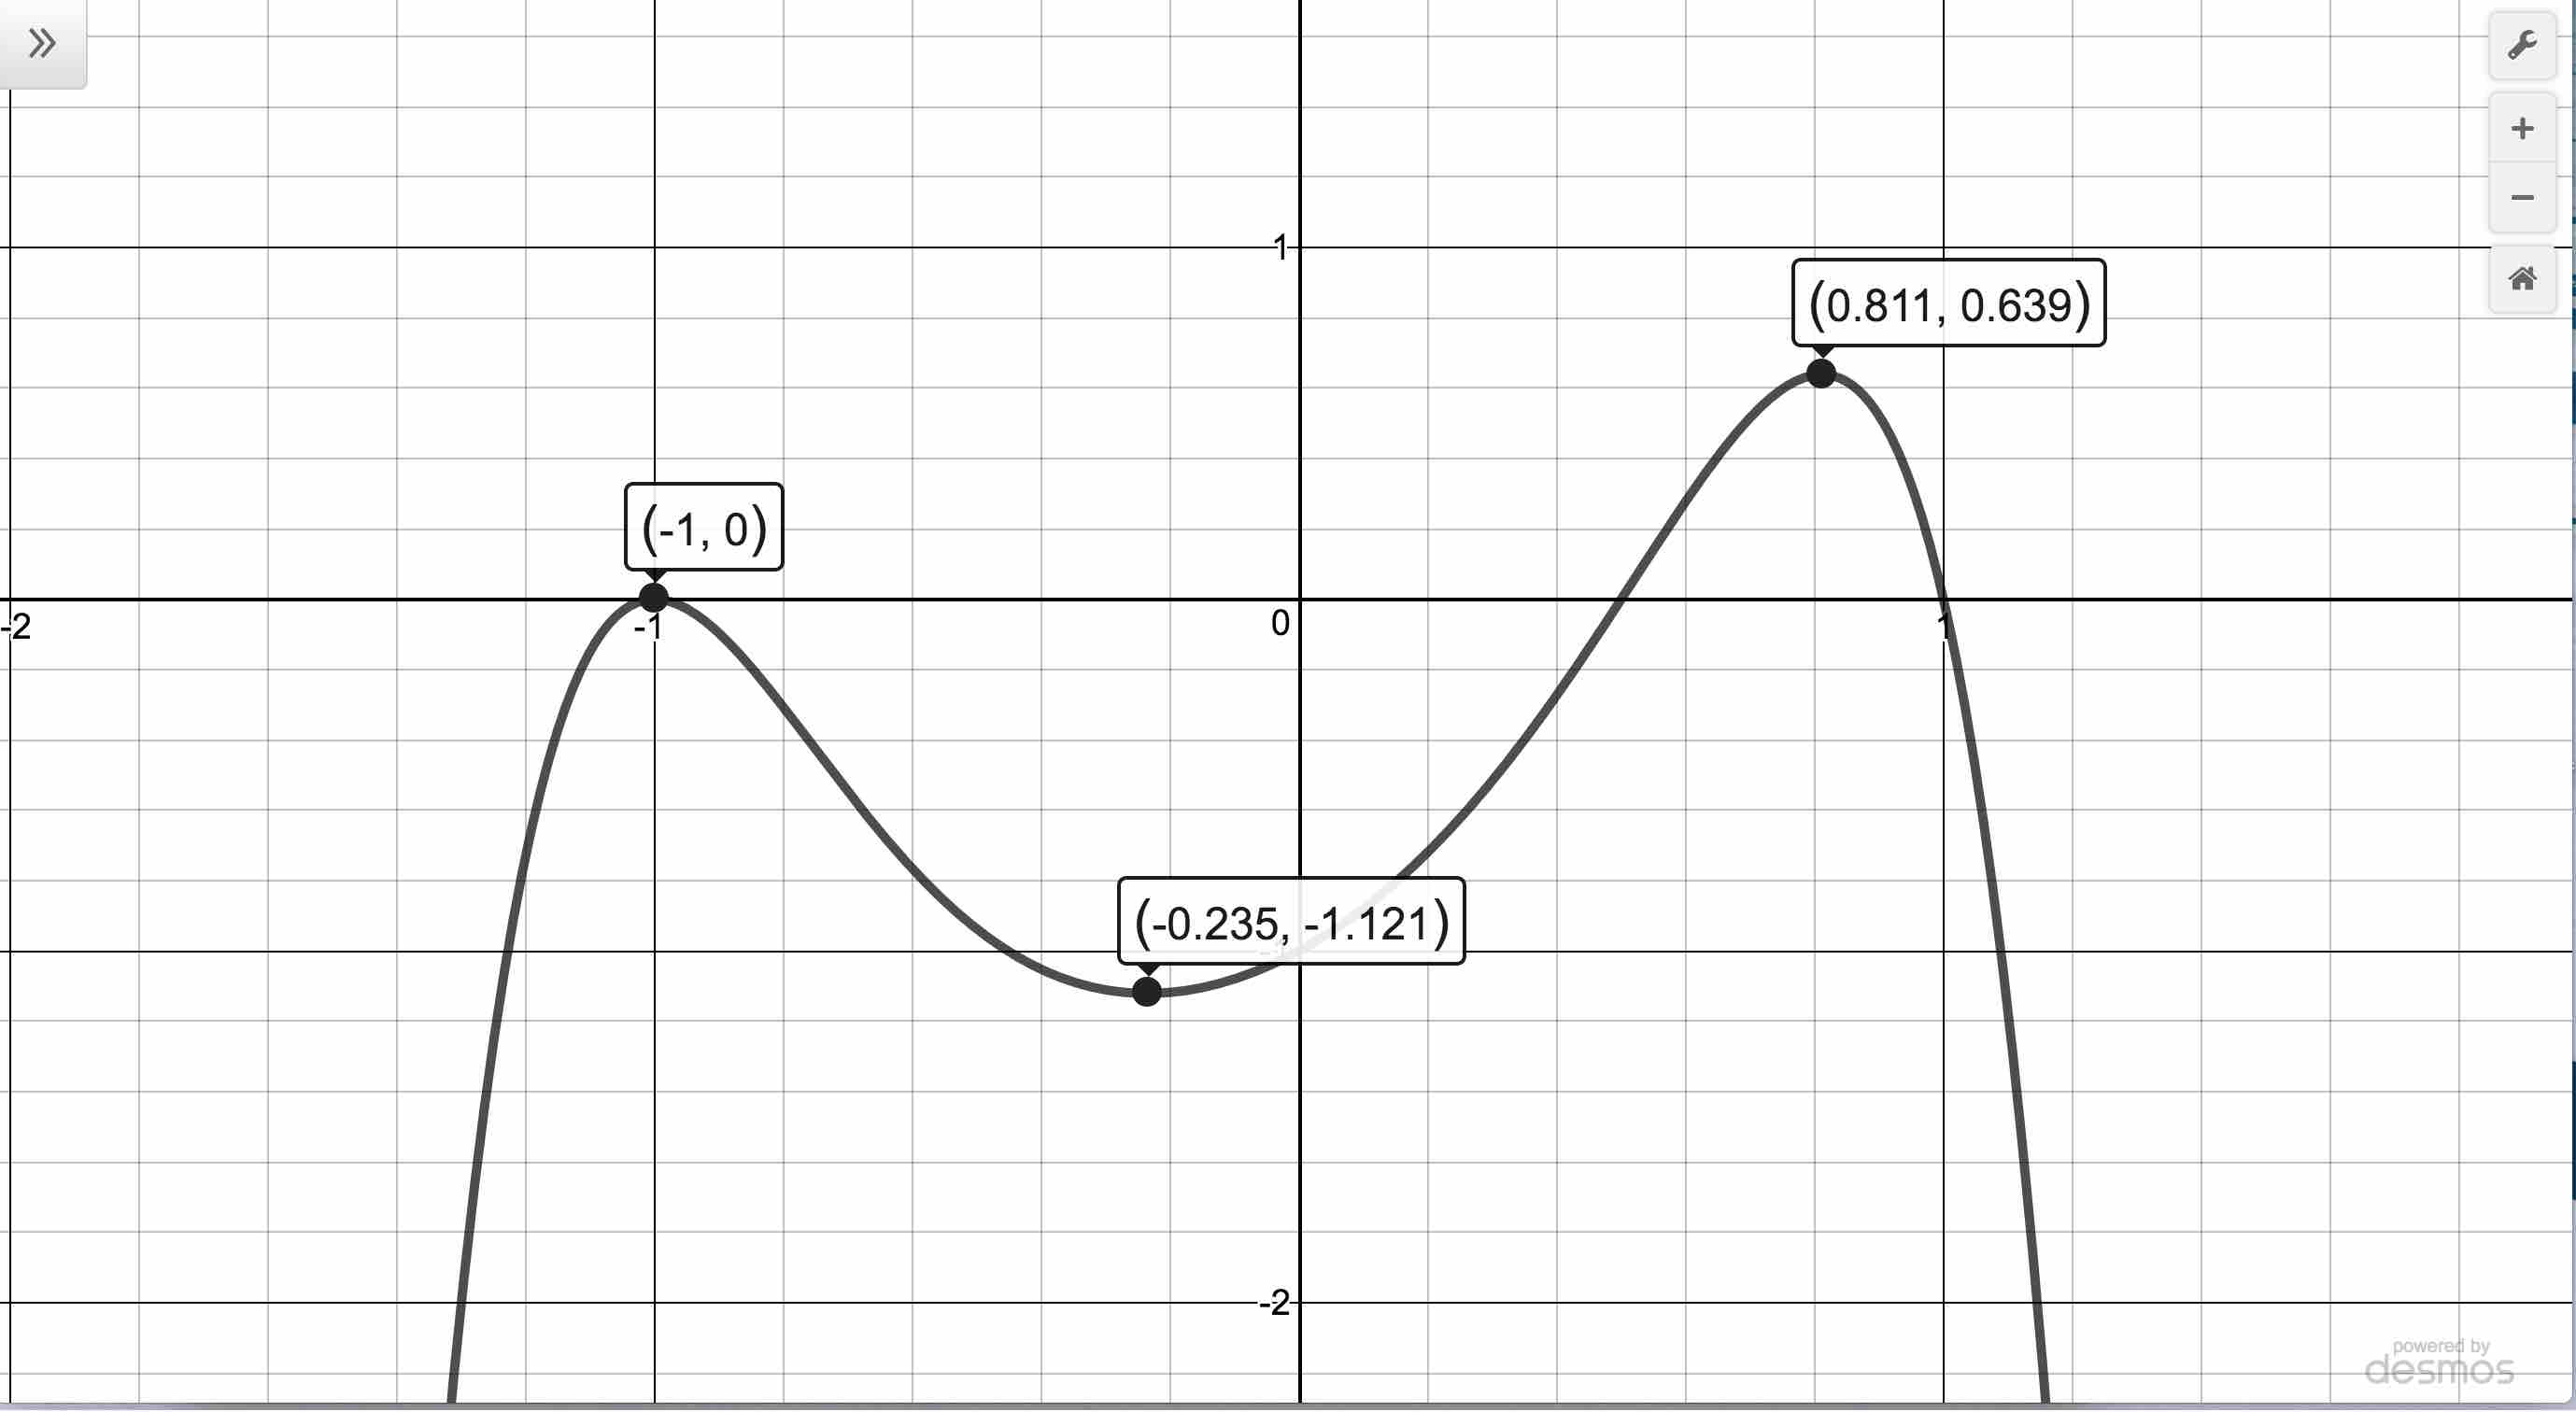
\includegraphics[width=6in]{./GraphsofPolynomialsGraphics/PolyRelativeExtrema.jpg} 

\end{center}



We close this section with a classic application of a third degree polynomial function.

\begin{ex}  \label{boxnotopex} A box with no top is to be fashioned from a $10$ inch $\times$ $12$ inch piece of cardboard by cutting out congruent squares from each corner of the cardboard and then folding the resulting tabs.  Let $x$ denote the length of the side of the square which is removed from each corner.

\bigskip

\begin{tabular}{m{1in}m{2.5in}m{2.5in}} 

&

\begin{mfpic}[15]{-2}{6}{-2}{7}
\hatchcolor[gray]{.7}
\lhatch \rect{(0,0),(1,1)}
\lhatch \rect{(0,5),(1,6)}
\lhatch \rect{(4,5),(5,6)}
\lhatch \rect{(4,0),(5,1)}
\polyline{(0,0),(5,0),(5,6),(0,6),(0,0)}
\dashed \polyline{(1,0),(1,1),(0,1)}
\dashed \polyline{(4,0),(4,1),(5,1)}
\dashed \polyline{(5,5),(4,5),(4,6)}
\dashed \polyline{(0,5),(1,5),(1,6)}
\dotted \polyline{(1,1),(4,1),(4,5),(1,5),(1,1)}
\tlabel[cc](0.5,1.25){\tiny $x$}
\tlabel[cc](1.25,0.5){\tiny $x$}
\tlabel[cc](4.5,1.25){\tiny $x$}
\tlabel[cc](3.75,0.5){\tiny $x$}
\tlabel[cc](4.5,4.75){\tiny $x$}
\tlabel[cc](3.75,5.5){\tiny $x$}
\tlabel[cc](0.5,4.75){\tiny $x$}
\tlabel[cc](1.25,5.5){\tiny $x$}
\arrow \reverse \arrow \polyline{(0,-0.5),(5,-0.5)}
\tlabel[cc](2.5,-1){\tiny $10$ in}
\arrow \reverse \arrow \polyline{(-0.5,0),(-0.5,6)}
\tlabel[cc](-1.5,3){\tiny $12$ in}
\end{mfpic}  & 

\begin{mfpic}[15]{-2}{8}{-2}{4}
\dashed \polyline{(0,1),(0,0)}
\dashed \polyline{(4,0), (4,1)}
\polyline{(0,1),(2,3)}
\polyline{(4,1),(6,3)}
\dotted \polyline{(0,0),(4,0)}
\polyline{(0,1),(4,1)}
\polyline{(2,3),(6,3)}
\dotted \polyline{(4,0),(6,2)}
\dashed \polyline{(6,3),(6,2)}
\dashed \polyline{(2,3),(2,2)}
\dotted \polyline{(2,2),(6,2)}
\dotted \polyline{(2,2),(0,0)}
\arrow \reverse \arrow \polyline{(0,-0.5),(4,-0.5)}
\tlabel[cc](2,-1){\tiny width}
\arrow \reverse \arrow \polyline{(-0.5,0), (-0.5,1)}
\tlabel[cc](-1.5,0.5){\tiny height}
\arrow \reverse \arrow \polyline{(4.5, -0.25), (6.5,1.75)}
\tlabel[cc](6,0.25){\tiny depth}
\end{mfpic}

\end{tabular}

\begin{enumerate}

\item  Find an expression for $V(x)$, the volume of the box produced by removing squares of edge length $x$. Include an appropriate domain.

\item  Use a graphing utility to help you determine the value of $x$ which produces the box with the largest volume.  What is the largest volume?  Round your answers to two decimal places.

\end{enumerate}

{\bf Solution.} 

\begin{enumerate}

\item  From Geometry, we know that $\text{Volume} = \text{width} \times \text{height} \times \text{depth}$.  The key is to find each of these quantities in terms of $x$.  From the figure, we see that the height of the box is $x$ itself.  The cardboard piece is initially $10$ inches wide.  Removing squares with a side length of $x$ inches from each corner leaves $10-2x$ inches for the width.\footnote{There's no harm in taking an extra step here and making sure this makes sense.  If we chopped out a $1$ inch square from each side, then the width would be $8$ inches, so chopping out $x$ inches would leave $10-2x$ inches.}  As for the depth, the cardboard is initially $12$ inches long, so after cutting out $x$ inches from each side, we would have $12-2x$ inches remaining. Hence, we get $V(x) = x(10-2x)(12-2x)$.  To find a suitable applied domain, we note that to make a box at all we need $x > 0$.  Also the shorter of the two dimensions of the cardboard is $10$ inches, and since we are removing $2x$ inches from this dimension, we also require $10 - 2x > 0$ or $x < 5$.  Hence, our applied domain is $0 < x < 5$.

\item  Using a graphing utility, we find a local maximum at approximately $(1.811, 96.771)$.  Because the domain of $V$ is restricted to the interval $(0,5)$,  the maximum of $V$ is here as well.

\begin{center}

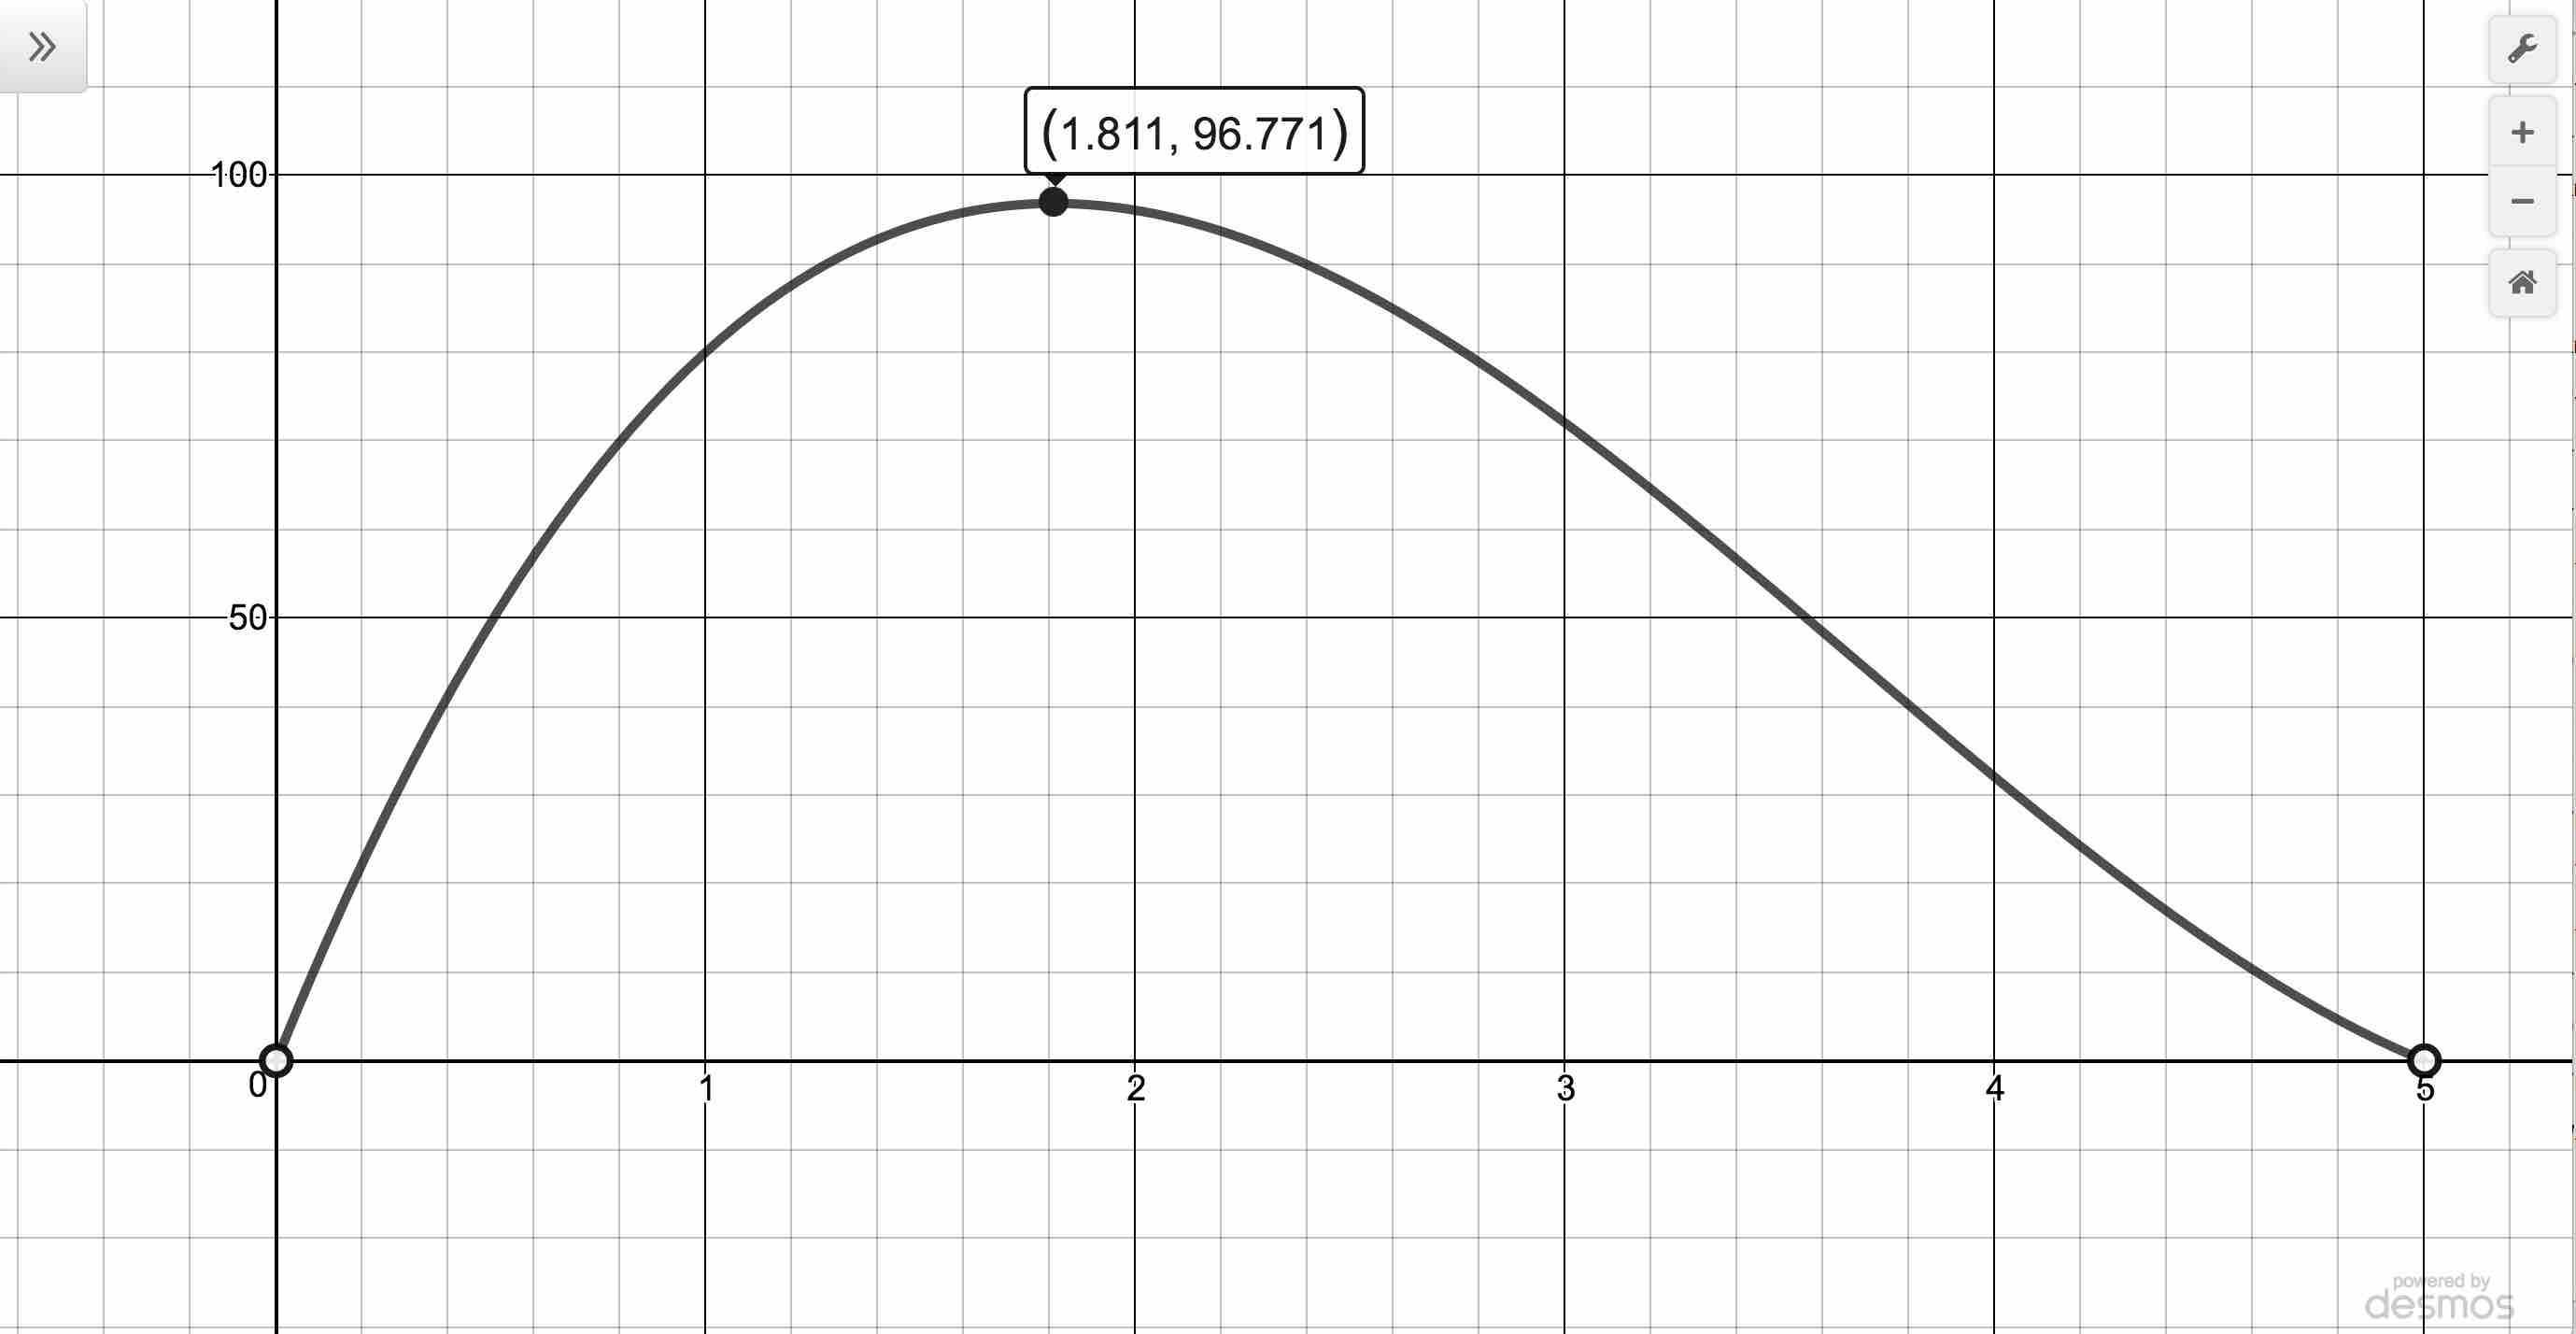
\includegraphics[width=6in]{./GraphsofPolynomialsGraphics/PolyBoxExample.jpg} 

\end{center}

This means the maximum volume attainable is approximately $96.77$ cubic inches when we remove squares approximately $1.81$ inches per side.\qed
 
\end{enumerate}
\label{openbox}
\end{ex}

Notice that there is a very slight, but important, difference between the function $V(x) = x(10-2x)(12-2x)$, $0 < x < 5$ from Example  \ref{boxnotopex} and the function $p(x) = x(10-2x)(12-2x)$: their domains.  The domain of $V$ is restricted to the interval $(0,5)$ while the domain of $p$ is $(-\infty, \infty)$.  Indeed, the function $V$ has a maximum of (approximately) $96.771$ at (approximately) $x = 1.811$ whereas for the function $p$, $96.771$ is a local maximum value only.  We leave it to the reader to verify that $V$ has neither a minimum nor a local minimum.

\newpage

\subsection{Exercises}

In Exercises \ref{polytransfirst} - \ref{polytranslast}, given the pair of functions $f$ and $F$, sketch the graph of $y=F(x)$ by starting with the graph of $y = f(x)$ and using Theorem \ref{linearmononialgraphs}.  Track at least three points of your choice through the transformations. State the domain and range of $g$.

\begin{multicols}{2}
\begin{enumerate}


\item $f(x) = x^3$,  $F(x) = (x + 2)^{3} + 1$ \label{polytransfirst}
\item $f(x) = x^4$, $F(x) = (x + 2)^{4} + 1$

\setcounter{HW}{\value{enumi}}
\end{enumerate}
\end{multicols}

\begin{multicols}{2}
\begin{enumerate}
\setcounter{enumi}{\value{HW}}

\item $f(x) = x^4$, $F(x) = 2 - 3(x - 1)^{4}$
\item $f(x) = x^5$, $F(x) = -x^{5} - 3$

\setcounter{HW}{\value{enumi}}
\end{enumerate}
\end{multicols}

\begin{multicols}{2}
\begin{enumerate}
\setcounter{enumi}{\value{HW}}

\item $f(x) = x^5$, $F(x) = (x+1)^5+10$
\item $f(x) = x^6$, $F(x) = 8-x^6$ \label{polytranslast}

\setcounter{HW}{\value{enumi}}
\end{enumerate}
\end{multicols}


In Exercises \ref{findformulaforcubicgraphfirst} - \ref{findformulacubicgraphlast}, find a formula for each function below in the form $F(x) = a(x-h)^3+k$.

\begin{multicols}{2}

\begin{enumerate}
\setcounter{enumi}{\value{HW}}

\item $~$ \label{findformulaforcubicgraphfirst}

\begin{mfpic}[15]{-5}{5}{-5}{5}
\axes
\tlabel[cc](5,-0.5){\scriptsize $x$}
\tlabel[cc](0.5,5){\scriptsize $y$}
\tlabel[cc](-1.25, -3){\scriptsize $(0,-3)$}
\tlabel[cc](1.25,-2.75){\scriptsize $(1,-2)$}
\xmarks{-4,-3,-2,-1,1,2,3,4}
\ymarks{-4,-3,-2, -1, 1,2,3,4}
\tlpointsep{4pt}
\scriptsize
\axislabels {x}{ {$-4 \hspace{7pt}$} -4, {$-3 \hspace{7pt}$} -3, {$-2 \hspace{7pt}$} -2, {$-1 \hspace{7pt}$} -1, {$1$} 1, {$2$} 2, {$3$} 3, {$4$} 4}
\axislabels {y}{{$-1$} -1,{$1$} 1, {$2$} 2, {$3$} 3, {$4$} 4, {$-2$} -2}
\penwd{1.25pt}
\arrow \reverse \arrow \function{-0.4,2.9,0.1}{(x-1)**3-2}
\point[4pt]{(1,-2), (0,-3)}
\tcaption{ \scriptsize$y = F(x)$}
\normalsize
\end{mfpic} 



\item $~$ \label{findformulacubicgraphlast}

\begin{mfpic}[15]{-5}{5}{-5}{5}
\axes
\tlabel[cc](5,-0.5){\scriptsize $x$}
\tlabel[cc](0.5,5){\scriptsize $y$}
\tlabel[cc](1,-1){\scriptsize $(0,-1)$}
\tlabel[cc](-2.25,2.25){\scriptsize $(-2,3)$}
\xmarks{-4,-3,-2,-1,1,2,3,4}
\ymarks{-4,-3,-2, -1, 1,2,3,4}
\tlpointsep{4pt}
\scriptsize
\axislabels {x}{ {$-4 \hspace{7pt}$} -4, {$-3 \hspace{7pt}$} -3, {$-2 \hspace{7pt}$} -2, {$-1 \hspace{7pt}$} -1, {$1$} 1, {$2$} 2, {$3$} 3, {$4$} 4}
\axislabels {y}{{$-1$} -1, {$2$} 2, {$3$} 3, {$4$} 4, {$-2$} -2, {$-3$} -3, {$-4$} -4}
\penwd{1.25pt}
\arrow \reverse \arrow \function{-3.5,0.5,0.1}{3-(0.5*((x+2)**3))}
\point[4pt]{(-2,3), (0,-1)}
\tcaption{ \scriptsize$y = F(x)$}
\normalsize
\end{mfpic} 

\setcounter{HW}{\value{enumi}}

\end{enumerate}

\end{multicols}

In Exercises \ref{findformulaforquartgraphfirst} - \ref{findformulaquartgraphlast}, find a formula for each function below in the form $F(x) = a(x-h)^4+k$.


\begin{multicols}{2}

\begin{enumerate}

\setcounter{enumi}{\value{HW}}

\item $~$ \label{findformulaforquartgraphfirst}

\begin{mfpic}[15]{-5}{5}{-5}{5}
\axes
\tlabel[cc](5,-0.5){\scriptsize $x$}
\tlabel[cc](0.5,5){\scriptsize $y$}
\tlabel[cc](-1.25,-4.5){\scriptsize $(-1,-4)$}
\tlabel[cc](1,-2){\scriptsize $(0,-2)$}
\xmarks{-4,-3,-2,-1,1,2,3,4}
\ymarks{-4,-3,-2, -1, 1,2,3,4}
\tlpointsep{4pt}
\scriptsize
\axislabels {x}{ {$-4 \hspace{7pt}$} -4, {$-3 \hspace{7pt}$} -3, {$-1 \hspace{7pt}$} -1, {$1$} 1, {$2$} 2,{$3$} 3, {$4$} 4}
\axislabels {y}{{$-1$} -1,{$1$} 1, {$2$} 2, {$3$} 3,  {$-2$} -2, {$-3$} -3, {$4$} 4}
\penwd{1.25pt}
\arrow \reverse \arrow \function{-2.41,0.41,0.1}{2*((x+1)**4)-4}
\point[4pt]{(-1,-4), (0,-2)}
\tcaption{ \scriptsize$y = F(x)$}
\normalsize
\end{mfpic} 



\item $~$  \label{findformulaquartgraphlast}

\begin{mfpic}[15]{-5}{5}{-5}{5}
\axes
\tlabel[cc](5,-0.5){\scriptsize $x$}
\tlabel[cc](0.5,5){\scriptsize $y$}
\tlabel[cc](-3,0.5){\scriptsize $(-2,0)$}
\tlabel[cc](2.5,0.5){\scriptsize $(2,0)$}
\tlabel[cc](-2,2.5){\scriptsize $(0,2.5)$}
\xmarks{-4,-3,-2,-1,1,2,3,4}
\ymarks{-4,-3,-2, -1, 1,2,3,4}
\tlpointsep{4pt}
\scriptsize
\axislabels {x}{ {$-4 \hspace{7pt}$} -4, {$-3 \hspace{7pt}$} -3, {$-1 \hspace{7pt}$} -1,  {$1$} 1, {$3$} 3, {$4$} 4}
\axislabels {y}{{$-1$} -1,{$-2$} -2,{$-3$} -3,{$-4$} -4,{$1$} 1, {$2$} 2, {$3$} 3,  {$4$} 4}
\penwd{1.25pt}
\arrow \reverse \arrow \function{-2.5,2.5,0.1}{2.5-(0.1565*(x**4))}
\point[4pt]{(-2,0), (2,0), (0, 2.5)}
\tcaption{ \scriptsize$y = F(x)$}
\normalsize
\end{mfpic} 


\setcounter{HW}{\value{enumi}}

\end{enumerate}

\end{multicols}


In Exercises \ref{polyfactsfirst} - \ref{polyfactslast}, find the degree, the leading term, the leading coefficient, the constant term and the end behavior of the given polynomial function.

\begin{multicols}{2}
\begin{enumerate}
\setcounter{enumi}{\value{HW}}
\item  $f(x) = 4-x-3x^2$ \label{polyfactsfirst}
\item  $g(x) = 3x^5 - 2x^2 + x + 1$

\setcounter{HW}{\value{enumi}}
\end{enumerate}
\end{multicols}

\begin{multicols}{2}
\begin{enumerate}
\setcounter{enumi}{\value{HW}}

\item $q(r) = 1 - 16r^{4}$
\item $Z(b) = 42b - b^{3}$

\setcounter{HW}{\value{enumi}}
\end{enumerate}
\end{multicols}

\begin{multicols}{2}
\begin{enumerate}
\setcounter{enumi}{\value{HW}}

\item $f(x) = \sqrt{3}x^{17} + 22.5x^{10} - \pi x^{7} + \frac{1}{3}$
\item $s(t) = -4.9t^{2} + v_{\mbox{\tiny $0$}}t + s_{\mbox{\tiny $0$}}$

\setcounter{HW}{\value{enumi}}
\end{enumerate}
\end{multicols}

\begin{multicols}{2}
\begin{enumerate}
\setcounter{enumi}{\value{HW}}

\item $P(x) = (x - 1)(x - 2)(x - 3)(x - 4)$
\item $p(t) = -t^2(3 - 5t)(t^{2} + t + 4)$

\setcounter{HW}{\value{enumi}}
\end{enumerate}
\end{multicols}

\begin{multicols}{2}
\begin{enumerate}
\setcounter{enumi}{\value{HW}}

\item $f(x) = -2x^3(x+1)(x+2)^2$
\item $G(t) = 4(t-2)^2\left(t+\frac{1}{2}\right)$ \label{polyfactslast}

\setcounter{HW}{\value{enumi}}
\end{enumerate}
\end{multicols}

\phantomsection
\label{polygraphexercise}

In Exercises \ref{zeromultgraphfirst} - \ref{zeromultgraphlast}, find the real zeros of the given polynomial and their corresponding multiplicities.  Use this information along with end behavior to provide a rough sketch of the graph of the polynomial function.  Compare your answer with the result from a graphing utility.

\begin{multicols}{2}
\begin{enumerate}
\setcounter{enumi}{\value{HW}}

\item $a(x) = x(x + 2)^{2}$ \label{zeromultgraphfirst}
\item $g(t) = t(t + 2)^{3}$

\setcounter{HW}{\value{enumi}}
\end{enumerate}
\end{multicols}


\begin{multicols}{2}
\begin{enumerate}
\setcounter{enumi}{\value{HW}}

\item $f(z) = -2(z-2)^2(z+1)$
\item $g(x) = (2x+1)^2(x-3)$

\setcounter{HW}{\value{enumi}}
\end{enumerate}
\end{multicols}


\begin{multicols}{2}
\begin{enumerate}
\setcounter{enumi}{\value{HW}}

\item $F(t) = t^{3}(t+ 2)^{2}$
\item $P(z) = (z- 1)(z - 2)(z - 3)(z - 4)$

\setcounter{HW}{\value{enumi}}
\end{enumerate}
\end{multicols}


\begin{multicols}{2}
\begin{enumerate}
\setcounter{enumi}{\value{HW}}

\item $Q(x) = (x + 5)^{2}(x - 3)^{4}$
\item $h(t) = t^2(t-2)^2(t+2)^2$

\setcounter{HW}{\value{enumi}}
\end{enumerate}
\end{multicols}


\begin{multicols}{2}
\begin{enumerate}
\setcounter{enumi}{\value{HW}}

\item $H(z) = (3-z)(z^2+1)$
\item $Z(x) = x(42 - x^{2})$ \label{zeromultgraphlast}

\setcounter{HW}{\value{enumi}}
\end{enumerate}
\end{multicols}

In Exercises \ref{evenoddornotpolyfirst} - \ref{evenoddornotpolylast}, determine analytically if the following functions are even, odd or neither.  Confirm your answer using a graphing utility.


\begin{multicols}{3}
\begin{enumerate}
\setcounter{enumi}{\value{HW}}

\item $f(x) = 7x$ \label{evenoddornotpolyfirst}
\item $g(t) = 7t + 2$
\item $p(z) = 7$

\setcounter{HW}{\value{enumi}}
\end{enumerate}
\end{multicols}

\begin{multicols}{3}
\begin{enumerate}
\setcounter{enumi}{\value{HW}}

\item $F(s) = 3s^2 - 4$
\item $h(t) = 4-t^2$
\item $g(x) = x^2-x-6$

\setcounter{HW}{\value{enumi}}
\end{enumerate}
\end{multicols}


\begin{multicols}{3}
\begin{enumerate}
\setcounter{enumi}{\value{HW}}

\item $f(x) = 2x^3 - x$
\item $p(z) = -z^5 + 2z^3 - z$
\item $G(t) = t^{6} - t^{4} + t^{2} + 9$

\setcounter{HW}{\value{enumi}}
\end{enumerate}
\end{multicols}

\begin{multicols}{3}
\begin{enumerate}
\setcounter{enumi}{\value{HW}}

\item $G(s) = s(s^2 - 1)$
\item $f(x) = (x^2+1)(x-1)$
\item $H(t) = (t^2-1)(t^4+t^2+3)$

\setcounter{HW}{\value{enumi}}
\end{enumerate}
\end{multicols}

\begin{multicols}{3}
\begin{enumerate}
\setcounter{enumi}{\value{HW}}

\item $g(t) = t(t-2)(t+2)$
\item $P(z) = (2z^{5} - 3z)(5z^3+z)$ 
\item $f(x) =0$  \label{evenoddornotpolylast}

\setcounter{HW}{\value{enumi}}
\end{enumerate}
\end{multicols}


\begin{enumerate}
\setcounter{enumi}{\value{HW}}

\item  \label{evenoddpolynomialexercise} Suppose $p(x)$ is a polynomial function written in the form of  Definition \ref{polynomialfunction}.  

\begin{enumerate}

\item  If the nonzero terms of $p(x)$ consist of even powers of $x$ (or a constant), explain why $p$ is even.

\item   If the nonzero terms of $p(x)$ consist of odd powers of $x$, explain why $p$ is odd.

\item  If $p(x)$ the nonzero terms of $p(x)$  contain at least one odd power of $x$ and one even power of $x$ (or a constant term), then $p$ is neither even nor odd.

\end{enumerate}

\newpage

\item  Use the results of Exercise \ref{evenoddpolynomialexercise} to determine whether the following functions are even, odd, or neither.

\begin{multicols}{4}
\begin{enumerate}

\item  $p(x) = 3x^4 + x^2 - 1$

\item  $F(s) = s^3 - 14s$

\item  $f(t) = 2t^5 - t^2 + 1$

\item  $g(x) =x^3(x^2+1)$

\end{enumerate}

\end{multicols}

\item  Show  $f(x) = |x|$ is an even function.


\item  Rework Example \ref{boxnotopex} assuming the box is to be made from an 8.5 inch by 11 inch sheet of paper. Using scissors and tape, construct the box.  Are you surprised?\footnote{Consider decorating the box and presenting it to your instructor. If done well enough, maybe your instructor will issue you some bonus points.  Or maybe not.}

\item For each function $f(x)$ listed below, compute the average rate of change over the indicated interval.\footnote{See Definition \ref{arc} in Section \ref{AverageRateofChange} for a review of this concept, as needed.}  What trends do you observe?  How do your answers manifest themselves graphically?

\[ \begin{array}{|r||c|c|c|c|c|c|}  \hline

 f(x) &  [-0.1, 0] & [0, 0.1] &[0.9, 1] & [1, 1.1] & [1.9, 2] & [2, 2.1]  \\ \hline
 1 &&&&&& \\  \hline
 x  &&&&&& \\  \hline
 x^2 &&&&&&  \\  \hline
 x^3 &&&&&& \\  \hline
 x^4 &&&&&& \\ \hline
 x^5 &&&&&& \\ \hline

\end{array} \]


\item \label{monomialarcexercise}For each function $f(x)$ listed below, compute the average rate of change over the indicated interval.\footnote{See Definition \ref{arc} in Section \ref{AverageRateofChange} for a review of this concept, as needed.}  What trends do you observe?  How do your answers manifest themselves graphically?

\[ \begin{array}{|r||c|c|c|c|}  \hline

 f(x) &  [0.9, 1.1] & [0.99, 1.01] &[0.999, 1.001] & [0.9999, 1.0001]  \\ \hline
 1 &&&&   \\  \hline
 x &&&&    \\  \hline
 x^2 &&&&   \\  \hline
 x^3 &&&&   \\  \hline
 x^4 &&&&  \\ \hline
 x^5 &&&&  \\ \hline

\end{array} \]




\setcounter{HW}{\value{enumi}}
\end{enumerate}

\phantomsection
\label{LCDmaxprofit} 

In Exercises \ref{lcdmaxprofitexerfirst} - \ref{lcdmaxprofitexerlast}, suppose the revenue $R$, in \textit{thousands} of dollars, from producing and selling $x$ \textit{hundred} LCD TVs is given by $R(x) = -5x^3+35x^2+155x$ for $0 \leq x \leq 10.07$.

\begin{enumerate}
\setcounter{enumi}{\value{HW}}

\item  Use a graphing utility to graph $y = R(x)$ and determine the number of TVs which should be sold to maximize revenue.  What is the maximum revenue? \label{lcdmaxprofitexerfirst}

\item Assume the cost, in \textit{thousands} of dollars, to produce $x$ \textit{hundred} LCD TVs is given by the function $C(x) = 200x + 25$ for $x \geq 0$. Find and simplify an expression for the profit function $P(x)$.  

(Remember: Profit = Revenue - Cost.)

\item  Use a graphing utility to graph $y = P(x)$ and determine the number of TVs which should be sold to maximize profit.  What is the maximum  profit? \label{lcdmaxprofitexerlast}

\item \label{newportaboycost} While developing their newest game, Sasquatch Attack!, the makers of the PortaBoy (from Example \ref{PortaBoyCost}) revised their cost function and now use $C(x) = .03x^{3} - 4.5x^{2} + 225x + 250$, for $x \geq 0$. As before, $C(x)$ is the cost to make $x$ PortaBoy Game Systems.  Market research indicates that the demand function $p(x) = -1.5x + 250$ remains unchanged.  Use a graphing utility to find the production level $x$ that maximizes the \textit{profit} made by producing and selling $x$ PortaBoy game systems.

\setcounter{HW}{\value{enumi}}
\end{enumerate}

\begin{enumerate}
\setcounter{enumi}{\value{HW}}

\item According to US Postal regulations, a rectangular shipping box must satisfy the following inequality: ``Length + Girth $\leq$ 130 inches'' for Parcel Post and ``Length + Girth $\leq$ 108 inches'' for other services. 

\smallskip

Let's assume we have a closed rectangular box with a square face of side length $x$ as drawn below.  The length is the longest side and is clearly labeled.  The girth is the distance around the box in the other two dimensions so in our case it is the sum of the four sides of the square, $4x$.  

\begin{enumerate}

\item \label{girthbox1} Assuming that we'll be mailing a box via Parcel Post where Length + Girth $=$ 130 inches, express the length of the box in terms of $x$ and then express the volume $V$ of the box in terms of $x$.

\item \label{girthbox2} Find the dimensions of the box of maximum volume that can be shipped via Parcel Post.

\item Repeat parts \ref{girthbox1} and \ref{girthbox2} if the box is shipped using ``other services''.

\end{enumerate}

\begin{center}

\begin{mfpic}[8]{-6}{12}{-1}{17}
\polyline{(0,0),(-4,3)}
\polyline{(-4,3), (-4,8)}
\polyline{(-4,8),(0,5)}
\polyline{(0,5),(0,0)}
\polyline{(0,0),(12,9)}
\polyline{(0,5),(12,14)}
\polyline{(-4,8),(8,17)}
\polyline{(8,17),(12,14)}
\polyline{(12,14),(12,9)}
\arrow \reverse \arrow \polyline{(0,-0.5),(12,8.5)}
\tlabel[cc](8,4){\tiny length}
\arrow \reverse \arrow \polyline{(-4, 2.5), (-0.5,-0.125)}
\tlabel[cc](-3,0.5){\tiny $x$}
\arrow \reverse \arrow \polyline{(-4.5, 3), (-4.5,8)}
\tlabel[cc](-5,5){\tiny $x$}
\end{mfpic}

\end{center}

\setcounter{HW}{\value{enumi}}
\end{enumerate}

\newpage

\begin{enumerate}
\setcounter{enumi}{\value{HW}}


\item \label{sunlighthigherorder} This exercise revisits the data set from Exercise \ref{regsunlight} in Section \ref{QuadraticFunctions}.  In that exercise, you were given a chart of the number of hours of daylight they get on the $21^{\mbox{st}}$ of each month in Fairbanks, Alaska based on the 2009 sunrise and sunset data found on the  \href{http://aa.usno.navy.mil/data/docs/RS_OneYear.php}{\underline{U.S. Naval Observatory}} website.  Here  $x = 1$ represents January 21, 2009, $x = 2$ represents February 21, 2009, and so on.  
\medskip

\small

\noindent \begin{tabular}{|l|r|r|r|r|r|r|r|r|r|r|r|r|} \hline
Month  & & & & & & & & & & & & \\
Number & 1 & 2 & 3 & 4 & 5 & 6 & 7 & 8 & 9 & 10 & 11 & 12\\ 
\hline 
Hours of  & & & & & & & & & & & & \\
Daylight & 5.8 & 9.3 & 12.4 & 15.9 & 19.4 & 21.8 & 19.4 & 15.6 & 12.4 & 9.1 & 5.6 & 3.3 \\ \hline
\end{tabular}

\normalsize

\medskip

\noindent 

\begin{itemize}

\item Find cubic (third degree) and quartic (fourth degree) polynomials which model this data and comment on the goodness of fit for each.  What can we say about using either model to make predictions about the year 2020?  (Hint: Think about the end behavior of polynomials.)  

\item Use the models to see how many hours of daylight they got on your birthday and then check the website to see how accurate the models are.  

\item Sasquatch are largely nocturnal, so what days of the year according to your models  allow for at least 14 hours of darkness for field research on the elusive creatures? 

\end{itemize}

\item \label{circuitexercisepoly} An electric circuit is built with a variable resistor installed.  For each of the following resistance values (measured in kilo-ohms, $k \Omega$),  the corresponding power to the load (measured in milliwatts, $mW$) is given in the table below. \footnote{The authors wish to thank Don Anthan and Ken White of Lakeland Community College for devising this problem and generating the accompanying data set.}

\noindent \begin{tabular}{|l|r|r|r|r|r|r|} \hline
Resistance: ($k \Omega$) & 1.012 & 2.199 & 3.275 & 4.676 & 6.805 & 9.975 \\ \hline
Power: ($mW$) & 1.063 & 1.496 & 1.610 & 1.613 & 1.505 & 1.314 \\ \hline
\end{tabular}

\begin{enumerate}

\item Make a scatter diagram of the data using the Resistance as the independent variable and Power as the dependent variable.

\item Use your calculator to find quadratic (2nd degree), cubic (3rd degree) and quartic (4th degree) regression models for the data and judge the reasonableness of each.

\item For each of the models found above, find the predicted maximum power that can be delivered to the load.  What is the corresponding resistance value?

\item Discuss with your classmates the limitations of these models - in particular, discuss the end behavior of each.

\end{enumerate}

\newpage

\item Below is a graph of  a polynomial function $y = p(x)$ as generated by a graphing utility.   Answer the following questions about $p$ based on the graph provided.


\centerline{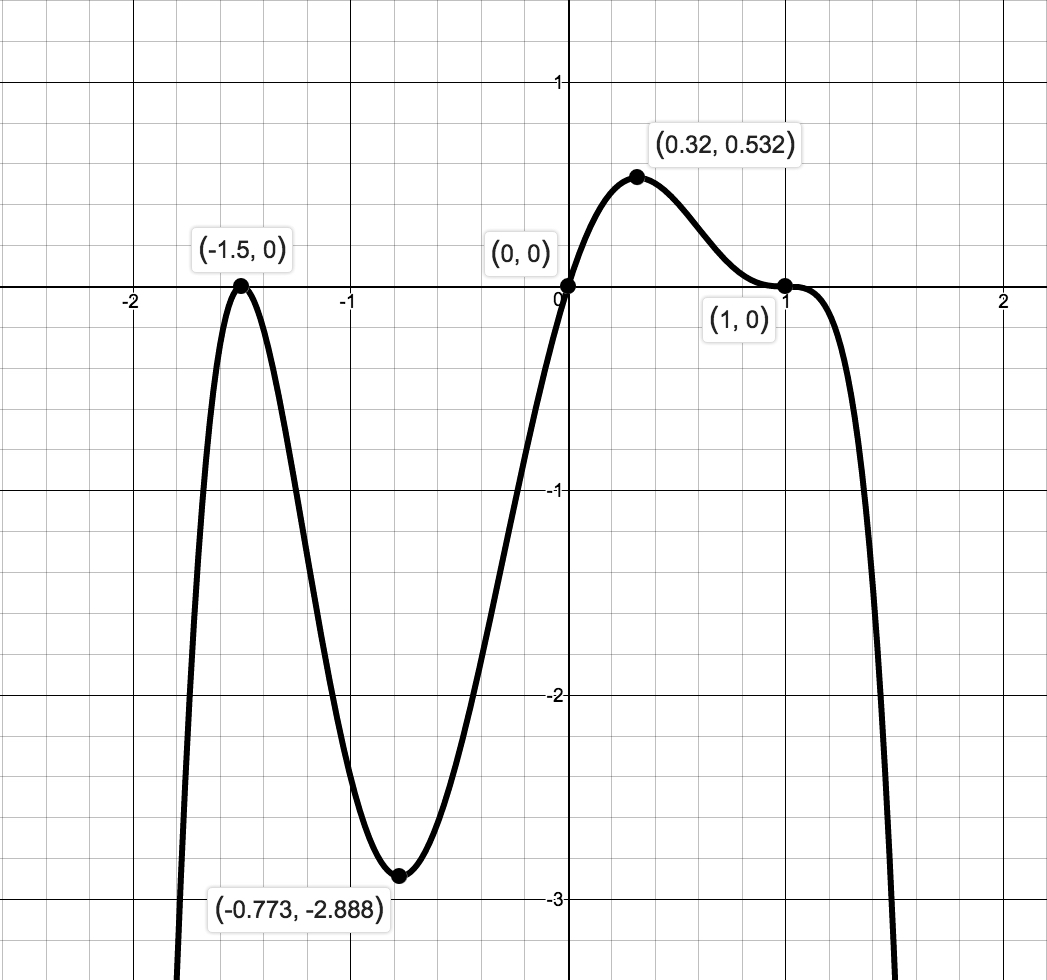
\includegraphics[width=3in]{./GraphsofPolynomialsGraphics/GraphsofPolyExercise.jpg}}

\begin{enumerate}

\item  Describe the end behavior of $y = p(x)$.

\item  List the real zeros of $p$ along with their respective multiplicities.  

\item  List the local minimums and local maximums of the graph of $y = p(x)$.

\item  What can be said about the degree of and leading coefficient $p(x)$?

\item  It turns out that $p(x)$ is a seventh degree polynomial.\footnote{to be exact, $p(x) = -0.1\left(x+1.5\right)^2\left(3x\right)\left(x-1\right)^3\left(x+5\right)$.}  How can this be?

\end{enumerate}

\item  \label{comparegraphfromtheoryexample}  (This Exercise is a follow up to Example \ref{graphfromtheory}.)  Use a graphing utility to  compare and contrast the graphs of $f(x) = (2x-1)(x+1)^2(1-x)(x^2+1)$ and $g(x) = (2x-1)(x+1)^2(1-x)$.

\item Use the graph of $y= p(x) = (2x-1)(x+1)(1-x^4)$ on page \pageref{localmaxminexample} to estimate the largest open interval containing $x = -0.235$ which satisfies the the criteria for `local minimum'  in Definition \ref{localmaxmindefn}.

\item  In light of Definition \ref{localmaxmindefn}, explain why \textit{every} point on the graph of a constant function is both a local maximum and a local minimum.

\item This exercise involves the greatest integer function, $f(x) = \lfloor x \rfloor$,  introduced in Example \ref{greatestintegerdefn}.  Explain why the points $(k,k)$ for integers $k$ are local maximums but not local minimums.

\item  Use Theorems  \ref{EBPolynomials}  and \ref{polynomialbehaviornearzeros} prove Theorem \ref{roleofmultiplicity}.


\newpage

\item Here are a few other questions for you to discuss with your classmates.  

\begin{enumerate}

\item How many and how few  local extrema could a polynomial of degree $n$ have?  
\item Could a polynomial have two local maxima but no local minima?  
\item If a polynomial has two local maxima and two local minima, can it be of odd degree?  Can it be of even degree?
\item Can a polynomial have local extrema without having any real zeros?
\item Why must every polynomial of odd degree have at least one real zero?
\item Can a polynomial have two distinct real zeros and no local extrema?
\item Can an $x$-intercept yield a local extrema?  Can it yield an absolute extrema?
\item If the $y$-intercept yields an absolute minimum, what can we say about the degree of the polynomial and the sign of the leading coefficient?   

\end{enumerate}

\item \label{LagrangePolyExercise} (This is a follow-up to Exercises \ref{LagrangeLinearExercise} in Section \ref{ConstantandLinearFunctions} and \ref{LagrangeQuadExercise} in Section \ref{QuadraticFunctions}.) The  \href{https://en.wikipedia.org/wiki/Lagrange_polynomial}{\underline{Lagrange Interpolate}} function $L$  for four  points:  $(x_{0}, y_{0})$, $(x_{1}, y_{1})$,  $(x_{2}, y_{2})$,   $(x_{3}, y_{3})$ where $x_{0}$,  $x_{1}$, $x_{2}$, and $x_{3}$ are four distinct real numbers is given by the formula: 

 \[ \begin{array}{rcl}
 
 L(x) & = &  y_{0}  \dfrac{(x - x_{1}) (x - x_{2}) (x-x_{3})}{(x_{0} - x_{1})(x_{0} - x_{2})(x_{0} - x_{3})}+ y_{1}  \dfrac{(x - x_{0}) (x - x_{2}) (x-x_{3})}{(x_{1} - x_{0})(x_{1} - x_{2})(x_{1} - x_{3})} \\ [15pt]
         &&  +y_{2}  \dfrac{(x - x_{0}) (x - x_{1}) (x-x_{3})}{(x_{2} - x_{0})(x_{2} - x_{1})(x_{2} - x_{3})}+ y_{3}  \dfrac{(x - x_{0}) (x - x_{1}) (x-x_{2})}{(x_{3} - x_{0})(x_{3} - x_{1})(x_{3} - x_{2})} \\ \end{array}\]

\begin{enumerate}

\item Choose four points with different $x$-values and construct the Lagrange Interpolate for those points.  Verify each of the points lies on the polynomial.  

\item  Verify that, in general, $L(x_{0}) = y_{0}$,  $L(x_{1}) = y_{1}$, $L(x_{2}) = y_{2}$, and  $L(x_{3}) = y_{3}$.

\item  Find $L(x)$ for the points $(-1,1)$, $(0,0)$,  $(1,1)$ and $(2,4)$.  What happens?

\item  Find $L(x)$ for the points $(-1,0)$, $(0,1)$,  $(1,2)$ and $(2,3)$.  What happens?

\item  Generalize the formula for $L(x)$ to five points.  What's the pattern?

\end{enumerate}

\setcounter{HW}{\value{enumi}}
\end{enumerate}
\newpage

\subsection{Answers}

\begin{multicols}{2}
\begin{enumerate}


\item $F(x) = (x + 2)^{3} + 1$ \\ 
domain: $(-\infty, \infty)$ \\ 
range: $(-\infty, \infty)$ \\

\begin{mfpic}[20][8]{-5}{1}{-11}{13}
\axes
\tlabel[cc](1,-0.75){\scriptsize $x$}
\tlabel[cc](0.5,13){\scriptsize $y$}
\point[4pt]{(-4,-7),(-3,0),(-2,1),(-1,2),(0,9)}
\xmarks{-4,-3,-2,-1}
\ymarks{-10 step 1 until 12}
\tiny
\tlpointsep{4pt}
\axislabels {x}{{$-4 \hspace{6pt}$} -4, {$-3 \hspace{6pt}$} -3, {$-2 \hspace{6pt}$} -2, {$-1 \hspace{6pt}$} -1}
\axislabels {y}{{$-10$} -10, {$-9$} -9, {$-8$} -8, {$-7$} -7, {$-6$} -6, {$-5$} -5, {$-4$} -4, {$-3$} -3, {$-2$} -2, {$-1$} -1, {$1$} 1, {$2$} 2, {$3$} 3, {$4$} 4, {$5$} 5, {$6$} 6, {$7$} 7, {$8$} 8, {$9$} 9, {$10$} 10, {$11$} 11, {$12$} 12}
\normalsize
\penwd{1.25pt}
\arrow \reverse \arrow \function{-4.25,0.25,0.1}{((x + 2)**3) + 1}
\end{mfpic}

\vfill

\columnbreak

\item $F(x) = (x + 2)^{4} + 1$\\
domain: $(-\infty, \infty)$\\
range: $[1, \infty)$\\

\begin{mfpic}[20][8]{-5}{1}{-1}{22}
\axes
\tlabel[cc](1,-0.75){\scriptsize $x$}
\tlabel[cc](0.5,22){\scriptsize $y$}
\point[4pt]{(-4,17),(-3,2),(-2,1),(-1,2),(0,17)}
\xmarks{-4,-3,-2,-1}
\ymarks{1 step 1 until 21}
\tiny
\tlpointsep{4pt}
\axislabels {x}{{$-4 \hspace{6pt}$} -4, {$-3 \hspace{6pt}$} -3, {$-2 \hspace{6pt}$} -2, {$-1 \hspace{6pt}$} -1}
\axislabels {y}{{$1$} 1, {$2$} 2, {$3$} 3, {$4$} 4, {$5$} 5, {$6$} 6, {$7$} 7, {$8$} 8, {$9$} 9, {$10$} 10, {$11$} 11, {$12$} 12, {$13$} 13, {$14$} 14, {$15$} 15, {$16$} 16, {$17$} 17, {$18$} 18, {$19$} 19, {$20$} 20, {$21$} 21}
\normalsize
\penwd{1.25pt}
\arrow \reverse \arrow \function{-4.12,0.12,0.1}{((x + 2)**4) + 1}
\end{mfpic}

\setcounter{HW}{\value{enumi}}
\end{enumerate}
\end{multicols}

\begin{multicols}{2}
\begin{enumerate}
\setcounter{enumi}{\value{HW}}


\item $F(x) = 2 - 3(x - 1)^{4}$\\
domain: $(-\infty, \infty)$\\
range: $(-\infty, 2]$\\

\begin{mfpic}[20][8]{-1}{3}{-14}{3}
\axes
\tlabel[cc](3,-0.75){\scriptsize $x$}
\tlabel[cc](0.5,3){\scriptsize $y$}
\point[4pt]{(1,2),(0,-1),(2,-1)}
\xmarks{1,2}
\ymarks{-13 step 1 until 2}
\tiny
\tlpointsep{4pt}
\axislabels {x}{{$1$} 1, {$2$} 2}
\axislabels {y}{{$-13$} -13, {$-12$} -12, {$-11$} -11, {$-10$} -10, {$-9$} -9, {$-8$} -8, {$-7$} -7, {$-6$} -6, {$-5$} -5, {$-4$} -4, {$-3$} -3, {$-2$} -2, {$-1$} -1, {$1$} 1, {$2$} 2}
\normalsize
\penwd{1.25pt}
\arrow \reverse \arrow \function{-0.5,2.5,0.1}{2 - 3*((x - 1)**4)}
\end{mfpic}


\vfill

\columnbreak

\item $F(x) = -x^{5} - 3$\\
domain: $(-\infty, \infty)$\\
range: $(-\infty, \infty)$\\

\begin{mfpic}[20][8]{-2}{2}{-11}{11}
\axes
\tlabel[cc](2,-0.75){\scriptsize $x$}
\tlabel[cc](0.5,11){\scriptsize $y$}
\point[4pt]{(-1,-2),(0,-3),(1,-4)}
\xmarks{-1,1}
\ymarks{-10 step 1 until 10}
\tiny
\tlpointsep{4pt}
\axislabels {x}{{$-1 \hspace{6pt}$} -1, {$1$} 1}
\axislabels {y}{{$-10$} -10, {$-9$} -9, {$-8$} -8, {$-7$} -7, {$-6$} -6, {$-5$} -5, {$-4$} -4, {$-3$} -3, {$-2$} -2, {$-1$} -1, {$1$} 1, {$2$} 2, {$3$} 3, {$4$} 4, {$5$} 5, {$6$} 6, {$7$} 7, {$8$} 8, {$9$} 9, {$10$} 10}
\normalsize
\penwd{1.25pt}
\arrow \reverse \arrow \function{-1.68,1.5,0.1}{-(x**5) - 3}
\end{mfpic}


\setcounter{HW}{\value{enumi}}
\end{enumerate}
\end{multicols}


\pagebreak

\begin{multicols}{2}
\begin{enumerate}

\setcounter{enumi}{\value{HW}}
\item $F(x) = (x+1)^5+10$\\
domain: $(-\infty, \infty)$\\
range: $(-\infty, \infty)$\\

\begin{mfpic}[20][8]{-5}{1}{-1}{22}
\axes
\tlabel[cc](1,-0.75){\scriptsize $x$}
\tlabel[cc](0.5,22){\scriptsize $y$}
\point[4pt]{(0,11), (-1,10), (-2,9)}
\xmarks{-4,-3,-2,-1}
\ymarks{1 step 1 until 21}
\tiny
\tlpointsep{4pt}
\axislabels {x}{{$-4 \hspace{6pt}$} -4, {$-3 \hspace{6pt}$} -3, {$-2 \hspace{6pt}$} -2, {$-1 \hspace{6pt}$} -1}
\axislabels {y}{{$1$} 1, {$2$} 2, {$3$} 3, {$4$} 4, {$5$} 5, {$6$} 6, {$7$} 7, {$8$} 8, {$9$} 9, {$10$} 10, {$11$} 11, {$12$} 12, {$13$} 13, {$14$} 14, {$15$} 15, {$16$} 16, {$17$} 17, {$18$} 18, {$19$} 19, {$20$} 20, {$21$} 21}
\normalsize
\penwd{1.25pt}
\arrow \reverse \arrow \function{-2.64,0.58,0.1}{((x + 1)**5) + 10}
\end{mfpic}


\vfill

\columnbreak

\item $F(x) = 8-x^{6}$\\
domain: $(-\infty, \infty)$\\
range: $(-\infty, 8]$\\

\begin{mfpic}[20][8]{-2}{2}{-11}{11}
\axes
\tlabel[cc](2,-0.75){\scriptsize $x$}
\tlabel[cc](0.5,11){\scriptsize $y$}
\point[4pt]{(-1,7),(0,8),(1,7)}
\xmarks{-1,1}
\ymarks{-10 step 1 until 10}
\tiny
\tlpointsep{4pt}
\axislabels {x}{{$-1 \hspace{6pt}$} -1, {$1$} 1}
\axislabels {y}{{$-10$} -10, {$-9$} -9, {$-8$} -8, {$-7$} -7, {$-6$} -6, {$-5$} -5, {$-4$} -4, {$-3$} -3, {$-2$} -2, {$-1$} -1, {$1$} 1, {$2$} 2, {$3$} 3, {$4$} 4, {$5$} 5, {$6$} 6, {$7$} 7, {$8$} 8, {$9$} 9, {$10$} 10}
\normalsize
\penwd{1.25pt}
\arrow \reverse \arrow \function{-1.6,1.6,0.1}{8-(x**6)}
\end{mfpic}


\setcounter{HW}{\value{enumi}}
\end{enumerate}
\end{multicols}


\begin{multicols}{2}
\begin{enumerate}
\setcounter{enumi}{\value{HW}}

\item  $F(x) = (x-1)^3-2$ \vphantom{$F(x) = -\frac{1}{2} (x+2)^3+3$}
\item $F(x) = -\frac{1}{2} (x+2)^3+3$

\setcounter{HW}{\value{enumi}}
\end{enumerate}
\end{multicols}

\begin{multicols}{2}
\begin{enumerate}
\setcounter{enumi}{\value{HW}}

\item  $F(x) = 2(x+1)^4-4$ \
\item $F(x) = -0.15625x^4+2.5$

\setcounter{HW}{\value{enumi}}
\end{enumerate}
\end{multicols}


\begin{multicols}{2}
\begin{enumerate}
\setcounter{enumi}{\value{HW}}
\item $f(x) = 4-x-3x^2$ \\
Degree 2 \\
Leading term $-3x^{2}$\\
Leading coefficient $-3$\\
Constant term $4$\\
As $x \rightarrow -\infty, \; f(x) \rightarrow -\infty$\\
As $x \rightarrow \infty, \; f(x) \rightarrow -\infty$\\

\item  $g(x) = 3x^5 - 2x^2 + x + 1$ \\
Degree 5 \\
Leading term $3x^5$\\
Leading coefficient $3$\\
Constant term $1$\\
As $x \rightarrow -\infty, \; g(x) \rightarrow -\infty$\\
As $x \rightarrow \infty, \; g(x) \rightarrow \infty$\\


\setcounter{HW}{\value{enumi}}
\end{enumerate}
\end{multicols}

\begin{multicols}{2}
\begin{enumerate}
\setcounter{enumi}{\value{HW}}

\item $q(r) = 1 - 16r^{4}$\\
Degree 4 \\
Leading term $-16r^{4}$\\
Leading coefficient $-16$\\
Constant term $1$\\
As $r \rightarrow -\infty, \; q(r) \rightarrow -\infty$\\
As $r \rightarrow \infty, \; q(r) \rightarrow -\infty$\\

\item $Z(b) = 42b - b^{3}$\\
Degree 3 \\
Leading term $-b^{3}$\\
Leading coefficient $-1$\\
Constant term $0$\\
As $b \rightarrow -\infty, \; Z(b) \rightarrow \infty$\\
As $b \rightarrow \infty, \; Z(b) \rightarrow -\infty$\\

\setcounter{HW}{\value{enumi}}
\end{enumerate}
\end{multicols}

\begin{multicols}{2}
\begin{enumerate}
\setcounter{enumi}{\value{HW}}

\item $f(x) = \sqrt{3}x^{17} + 22.5x^{10} - \pi x^{7} + \frac{1}{3}$\\
Degree 17 \\
Leading term $\sqrt{3}x^{17}$\\
Leading coefficient $\sqrt{3}$\\
Constant term $\frac{1}{3}$\\
As $x \rightarrow -\infty, \; f(x) \rightarrow -\infty$\\
As $x \rightarrow \infty, \; f(x) \rightarrow \infty$\\


\item $s(t) = -4.9t^{2} + v_{\mbox{\tiny $0$}}t + s_{\mbox{\tiny $0$}}$\\
Degree 2 \\
Leading term $-4.9t^{2}$\\
Leading coefficient $-4.9$\\
Constant term $s_{\mbox{\tiny $0$}}$\\
As $t \rightarrow -\infty, \; s(t) \rightarrow -\infty$\\
As $t \rightarrow \infty, \; s(t) \rightarrow -\infty$\\


\setcounter{HW}{\value{enumi}}
\end{enumerate}
\end{multicols}

\begin{multicols}{2}
\begin{enumerate}
\setcounter{enumi}{\value{HW}}


\item $P(x) = (x - 1)(x - 2)(x - 3)(x - 4)$\\
Degree 4 \\
Leading term $x^{4}$\\
Leading coefficient $1$\\
Constant term $24$\\
As $x \rightarrow -\infty, \; P(x) \rightarrow \infty$\\
As $x \rightarrow \infty, \; P(x) \rightarrow \infty$\\

\item $p(t) = -t^2(3 - 5t)(t^{2} + t + 4)$\\
Degree 5 \\
Leading term $5t^{5}$\\
Leading coefficient $5$\\
Constant term $0$\\
As $t \rightarrow -\infty, \; p(t) \rightarrow -\infty$\\
As $t \rightarrow \infty, \; p(t) \rightarrow \infty$\\

\setcounter{HW}{\value{enumi}}
\end{enumerate}
\end{multicols}



\begin{multicols}{2}
\begin{enumerate}
\setcounter{enumi}{\value{HW}}

\item $f(x) = -2x^3(x+1)(x+2)^2$ \\
Degree 6 \\
Leading term $-2x^{6}$\\
Leading coefficient $-2$\\
Constant term $0$\\
As $x \rightarrow -\infty, \; f(x) \rightarrow -\infty$\\
As $x \rightarrow \infty, \; f(x) \rightarrow -\infty$\\

\item $G(t) = 4(t-2)^2\left(t+\frac{1}{2}\right)$ \\
Degree 3 \\
Leading term $4t^3$\\
Leading coefficient $4$\\
Constant term $8$\\
As $t \rightarrow -\infty, \; G(t) \rightarrow -\infty$\\
As $t \rightarrow \infty, \; G(t) \rightarrow \infty$\\

\setcounter{HW}{\value{enumi}}
\end{enumerate}
\end{multicols}

\begin{multicols}{2}
\begin{enumerate}
\setcounter{enumi}{\value{HW}}

\item $a(x) = x(x + 2)^{2}$\\
$x = 0$ multiplicity 1\\
$x = -2$ multiplicity 2\\

\begin{mfpic}[20][10]{-3}{1}{-3}{5}
\axes
\tlabel[cc](1,-0.5){\scriptsize $x$}
\tlabel[cc](0.25,5){\scriptsize $y$}
\point[4pt]{(-2,0), (0,0)}
\xmarks{-2,-1}
\tiny
\tlpointsep{4pt}
\axislabels {x}{{$-2 \hspace{6pt}$} -2, {$-1 \hspace{6pt}$} -1}
\normalsize
\penwd{1.25pt}
\arrow \reverse \arrow \function{-3,0.65,0.1}{x*((x + 2)**2)}
\end{mfpic}

\vfill

\columnbreak

\item $g(t) = t(t + 2)^{3}$\\
$t = 0$ multiplicity 1\\
$t = -2$ multiplicity 3\\

\begin{mfpic}[20][20]{-3}{1}{-2}{5}
\axes
\tlabel[cc](1,-0.5){\scriptsize $t$}
\tlabel[cc](0.25,5){\scriptsize $y$}
\point[4pt]{(-2,0), (0,0)}
\xmarks{-2,-1}
\tiny
\tlpointsep{4pt}
\axislabels {x}{{$-2 \hspace{6pt}$} -2, {$-1 \hspace{6pt}$} -1}
\normalsize
\penwd{1.25pt}
\arrow \reverse \arrow \function{-3,0.3,0.1}{x*((x + 2)**3)}
\end{mfpic}


\setcounter{HW}{\value{enumi}}
\end{enumerate}
\end{multicols}

\begin{multicols}{2}
\begin{enumerate}
\setcounter{enumi}{\value{HW}}

\item $f(z) = -2(z-2)^2(z+1)$\\
$z=2$ multiplicity 2 \\
$z=-1$ multiplicity 1\\

\begin{mfpic}[20][10]{-3}{3}{-4}{4}
\axes
\tlabel[cc](3,-0.5){\scriptsize $z$}
\tlabel[cc](0.25,4){\scriptsize $y$}
\point[4pt]{(2,0), (-1,0)}
\xmarks{-2,-1,1,2}
\tiny
\tlpointsep{4pt}
\axislabels {x}{{$-2 \hspace{6pt}$} -2, {$-1 \hspace{6pt}$} -1, {$1$} 1, {$2$} 2}
\normalsize
\penwd{1.25pt}
\arrow \reverse \arrow \function{-1.70,3.45,0.1}{(-0.4)*((x-2)**2)*(x+1)}
\end{mfpic}



\item $g(x) = (2x+1)^2(x-3)$\\
$x=-\frac{1}{2}$ multiplicity 2 \\
$x=3$ multiplicity 1\\

\begin{mfpic}[20][10]{-2}{4}{-4}{4}
\axes
\tlabel[cc](4,-0.5){\scriptsize $x$}
\tlabel[cc](0.25,4){\scriptsize $y$}
\point[4pt]{(-0.5,0), (3,0)}
\xmarks{-1,1,2,3}
\tiny
\tlpointsep{4pt}
\axislabels {x}{{$-1 \hspace{6pt}$} -1, {$1$} 1, {$2$} 2, {$3$} 3}
\normalsize
\penwd{1.25pt}
\arrow \reverse \arrow \function{-1.5,3.3,0.1}{(0.5)*((x+0.5)**2)*(x-3)}
\end{mfpic}



\setcounter{HW}{\value{enumi}}
\end{enumerate}
\end{multicols}



\begin{multicols}{2}
\begin{enumerate}
\setcounter{enumi}{\value{HW}}

\item $F(t) = t^{3}(t + 2)^{2}$\\
$t = 0$ multiplicity 3\\
$t = -2$ multiplicity 2\\

\begin{mfpic}[20][10]{-3}{1}{-3}{5}
\axes
\tlabel[cc](1,-0.5){\scriptsize $t$}
\tlabel[cc](0.25,5){\scriptsize $y$}
\point[4pt]{(-2,0), (0,0)}
\xmarks{-2,-1}
\tiny
\tlpointsep{4pt}
\axislabels {x}{{$-2 \hspace{6pt}$} -2, {$-1 \hspace{6pt}$} -1}
\normalsize
\penwd{1.25pt}
\arrow \reverse \arrow \function{-2.45,0.85,0.1}{(x**3)*((x + 2)**2)}
\end{mfpic}

\vfill

\columnbreak

\item $P(z) = (z - 1)(z - 2)(z - 3)(z - 4)$\\
$z = 1$ multiplicity 1\\
$z = 2$ multiplicity 1\\
$z = 3$ multiplicity 1\\
$z = 4$ multiplicity 1\\

\begin{mfpic}[20][10]{0}{5}{-1}{5}
\axes
\tlabel[cc](5,-0.5){\scriptsize $z$}
\tlabel[cc](0.25,5){\scriptsize $y$}
\point[4pt]{(1,0),(2,0),(3,0),(4,0)}
\xmarks{1,2,3,4}
\tiny
\tlpointsep{4pt}
\axislabels {x}{{$1$} 1, {$2$} 2, {$3$} 3, {$4$} 4}
\normalsize
\penwd{1.25pt}
\arrow \reverse \arrow \function{0.6,4.4,0.1}{(x - 1)*(x - 2)*(x - 3)*(x - 4)}
\end{mfpic}

\setcounter{HW}{\value{enumi}}
\end{enumerate}
\end{multicols}


\begin{multicols}{2}
\begin{enumerate}
\setcounter{enumi}{\value{HW}}


\item $Q(x) = (x + 5)^{2}(x - 3)^{4}$\\
$x = -5$ multiplicity 2\\
$x = 3$ multiplicity 4\\

\begin{mfpic}[10][20]{-6}{6}{-1}{3}
\axes
\tlabel[cc](6,-0.5){\scriptsize $x$}
\tlabel[cc](0.5,3){\scriptsize $y$}
\point[4pt]{(-5,0),(3,0)}
\xmarks{-5 step 1 until 5}
\tiny
\tlpointsep{4pt}
\axislabels {x}{{$-5 \hspace{6pt}$} -5, {$-4 \hspace{6pt}$} -4, {$-3 \hspace{6pt}$} -3, {$-2 \hspace{6pt}$} -2, {$-1 \hspace{6pt}$} -1, {$1$} 1, {$2$} 2, {$3$} 3, {$4$} 4, {$5$} 5}
\normalsize
\penwd{1.25pt}
\arrow \reverse \arrow \function{-5.9,5.6,0.1}{(((x + 5)**2)*((x - 3)**4))/2000}
\end{mfpic}

\vfill

\columnbreak

\item $f(t) = t^2(t-2)^2(t+2)^2$\\
$t = -2$ multiplicity 2\\
$t = 0$ multiplicity 2\\
$t = 2$ multiplicity 2\\

\begin{mfpic}[20][10]{-3}{3}{-1}{5}
\axes
\tlabel[cc](3,-0.5){\scriptsize $t$}
\tlabel[cc](0.5,5){\scriptsize $y$}
\point[4pt]{(-2,0), (0,0), (2,0)}
\xmarks{-2 step 1 until 2}
\tiny
\tlpointsep{4pt}
\axislabels {x}{{$-2 \hspace{6pt}$} -2, {$-1 \hspace{6pt}$} -1, {$1$} 1, {$2$} 2}
\normalsize
\penwd{1.25pt}
\arrow \reverse \arrow \function{-2.45,2.45,0.1}{(0.2)*(x**2)*((x-2)**2)*((x+2)**2)}
\end{mfpic}

\setcounter{HW}{\value{enumi}}
\end{enumerate}
\end{multicols}

\begin{multicols}{2}
\begin{enumerate}
\setcounter{enumi}{\value{HW}}

\item $H(z) = (3-z)\left(z^2+1\right)$\\
$z=3$ multiplicity 1\\

\begin{mfpic}[20][10]{-1}{4}{-4}{4}
\axes
\tlabel[cc](4,-0.5){\scriptsize $z$}
\tlabel[cc](0.5,3){\scriptsize $y$}
\point[4pt]{(3,0)}
\xmarks{1 step 1 until 3}
\tiny
\tlpointsep{4pt}
\axislabels {x}{{$1$} 1, {$2$} 2, {$3$} 3}
\normalsize
\penwd{1.25pt}
\arrow \reverse \arrow \function{-0.75,3.3,0.1}{(0.5)*(3-x)*((x**2)+1)}
\end{mfpic}

\vfill

\columnbreak

\item $Z(x) = x(42 - x^{2})$\\
$x = -\sqrt{42}$  multiplicity 1\\
$x = 0$ multiplicity 1\\
$x = \sqrt{42}$ multiplicity 1\\

\begin{mfpic}[10]{-7}{7}{-6}{6}
\axes
\tlabel[cc](7,-0.5){\scriptsize $x$}
\tlabel[cc](0.5,6){\scriptsize $y$}
\point[4pt]{(-6.4807,0),(0,0),(6.4807,0)}
\xmarks{-6 step 1 until 6}
\tiny
\tlpointsep{4pt}
\axislabels {x}{{$-6 \hspace{6pt}$} -6, {$-5 \hspace{6pt}$} -5, {$-4 \hspace{6pt}$} -4, {$-3 \hspace{6pt}$} -3, {$-2 \hspace{6pt}$} -2, {$-1 \hspace{6pt}$} -1, {$1$} 1, {$2$} 2, {$3$} 3, {$4$} 4, {$5$} 5, {$6$} 6}
\normalsize
\penwd{1.25pt}
\arrow \reverse \arrow \function{-7,7,0.1}{(42*x - x**3)/20}
\end{mfpic}

\setcounter{HW}{\value{enumi}}
\end{enumerate}
\end{multicols}

\begin{multicols}{3}
\begin{enumerate}
\setcounter{enumi}{\value{HW}}

\item odd
\item neither
\item even

\setcounter{HW}{\value{enumi}}
\end{enumerate}
\end{multicols}

\begin{multicols}{3}
\begin{enumerate}
\setcounter{enumi}{\value{HW}}

\item even
\item even
\item neither

\setcounter{HW}{\value{enumi}}
\end{enumerate}
\end{multicols}


\begin{multicols}{3}
\begin{enumerate}
\setcounter{enumi}{\value{HW}}

\item odd
\item odd
\item even

\setcounter{HW}{\value{enumi}}
\end{enumerate}
\end{multicols}

\begin{multicols}{3}
\begin{enumerate}
\setcounter{enumi}{\value{HW}}

\item odd
\item neither
\item even

\setcounter{HW}{\value{enumi}}
\end{enumerate}
\end{multicols}

\begin{multicols}{3}
\begin{enumerate}
\setcounter{enumi}{\value{HW}}

\item odd
\item even
\item even  \textbf{and} odd

\setcounter{HW}{\value{enumi}}
\end{enumerate}
\end{multicols}

\begin{enumerate}
\setcounter{enumi}{\value{HW}}

\addtocounter{enumi}{1}

\item  \begin{multicols}{4}
\begin{enumerate}

\item even

\item  odd

\item  neither

\item  odd\footnote{You need to first multiply out the expression for $g(x)$ so it is in the form prescribed by Definition \ref{polynomialfunction}.}

\end{enumerate}

\end{multicols}

\item For $f(x) = |x|$, $f(-x) = |-x| = |(-1) x|  = |-1| |x| = (1) |x| = |x|$.  Hence, $f(-x) = f(x)$.

\item  $V(x) = x(8.5-2x)(11-2x) = 4x^3-39x^2+93.5x$, $0 < x < 4.25$.  Volume is maximized when $x \approx 1.58$, so we get the dimensions of the box with maximum volume are: height $\approx$ 1.58 inches, width $\approx$ 5.34 inches, and depth $\approx$ 7.84 inches.  The maximum volume is $\approx$ 66.15 cubic inches.

\item  Each of these average rates of change indicate slope of the curve over the given interval.  Smaller slopes correspond to `flatter' curves and higher slopes correspond to `steeper' curves.

\[ \begin{array}{|r||c|c|c|c|c|c|}  \hline

 f(x) &  [-0.1, 0] & [0, 0.1] &[0.9, 1] & [1, 1.1] & [1.9, 2] & [2, 2.1]  \\ \hline
 1 &  0 &   0  & 0   & 0   & 0  & 0 \\  \hline
 x &  1 &   1  & 1   & 1   & 1  & 1 \\  \hline
 x^2 & -0.1 & 0.1 & 1.9 & 2.1 & 3.9 & 4.1  \\  \hline
 x^3 & 0.01  & 0.01 & 2.71 & 3.31 & 11.41 & 12.61 \\  \hline
 x^4&  -0.001 & 0.001 & 3.439 & 4.641 & 29.679 & 34.481 \\ \hline
 x^5 & 0.0001 & 0.0001 & 4.0951 & 6.1051 & 72.3901 & 88.4101 \\ \hline

\end{array} \]


\item As we sample points closer to $x=1$, the slope of the curve approaches the exponent on $x$.

\[ \begin{array}{|r||c|c|c|c|}  \hline

 f(x) &  [0.9, 1.1] & [0.99, 1.01] &[0.999, 1.001] & [0.9999, 1.0001]  \\ \hline
 1 &  0 &   0  & 0   & 0   \\  \hline
 x &  1 &   1  & 1   & 1   \\  \hline
 x^2 & 2 & 2 & 2 & 2  \\  \hline
 x^3 & 3.01  & 3.0001 & \approx 3 & \approx 3  \\  \hline
 x^4&  4.04 & 4.0004 & \approx 4 & \approx 4 \\ \hline
 x^5 & 5.1001 & \approx 5.001 & \approx 5 & \approx 5  \\ \hline

\end{array} \]


\item The calculator gives the location  of the absolute maximum (rounded to three decimal places) as $x \approx 6.305$ and $y \approx 1115.417$.  Since $x$ represents the number of TVs sold in hundreds, $x = 6.305$ corresponds to $630.5$ TVs.  Since we can't sell half of a TV, we compare $R(6.30) \approx 1115.415$ and $R(6.31) \approx 1115.416$, so selling $631$ TVs results in a (slightly) higher revenue.  Since $y$ represents the revenue in \textit{thousands} of dollars, the maximum revenue is $\$ 1,\!115,\!416$.

\item $P(x) = R(x) - C(x) = -5x^3+35x^2-45x-25$, $0 \leq x \leq 10.07$.

\item  The calculator gives the location  of the absolute maximum (rounded to three decimal places) as $x \approx 3.897$ and $y \approx 35.255$.  Since $x$ represents the number of TVs sold in hundreds, $x = 3.897$ corresponds to $389.7$ TVs.  Since we can't sell $0.7$ of a TV, we compare $P(3.89) \approx 35.254$ and $P(3.90) \approx 35.255$, so selling $390$ TVs results in a (slightly) higher revenue.  Since $y$ represents the revenue in \textit{thousands} of dollars, the maximum revenue is $\$ 35,\!255$.

\item Making and selling 71 PortaBoys yields a maximized profit of \$5910.67.


\item \begin{enumerate}

\item To maximize the volume, we assume we start with the maximum Length $+$ Girth of $130$,  so the length is $130 - 4x$.  The volume of a rectangular box is  `length $\times$ width $\times$ height' so we get $V(x) = x^{2}(130 - 4x) = -4x^{3} + 130x^{2}$.  

\item Using a graphing utility, we get a (local) maximum of  $y = V(x)$ at $(21.67, 20342.59)$.  Hence, the maximum volume is $20342.59\mbox{in.}^{3}$ using a box with dimensions $21.67\mbox{in.} \times 21.67\mbox{in.} \times 43.32\mbox{in.}$.

\item If we start with Length $+$ Girth $= 108$ then the length is $108 - 4x$ so  $V(x) = -4x^{3} + 108x^{2}$.  Graphing $y = V(x)$  shows a (local) maximum at $(18.00, 11664.00)$ so the dimensions of the box with maximum volume are $18.00\mbox{in.} \times 18.00\mbox{in.} \times 36\mbox{in.}$ for a volume of $11664.00\mbox{in.}^{3}$.  (Calculus will confirm that the measurements which maximize the volume are \underline{exactly} 18in. by 18in. by 36in., however, as I'm sure you are aware by now, we treat all numerical results as approximations and list them as such.)

\end{enumerate}

\setcounter{HW}{\value{enumi}}
\end{enumerate}




\begin{enumerate}
\setcounter{enumi}{\value{HW}}


\item \begin{itemize} \item The cubic regression model is $p_{\mbox{\tiny $3$}}(x) = 0.0226x^{3} - 0.9508x^{2} + 8.615x - 3.446$.  It has $R^{2} = 0.9377$ which isn't bad.  The graph of $y = p_{\mbox{\tiny $3$}}(x)$ along with the data is shown below on the left.  Note $p_{\mbox{\tiny $3$}}$ hits the $x$-axis at about $x = 12.45$ making this a bad model for future predictions.  

\item To use the model to approximate the number of hours of sunlight on your birthday, you'll have to figure out what decimal value of $x$ is close enough to your birthday and then plug it into the model.  Jeff's birthday is July 31 which is 10 days after July 21 ($x = 7$).  Assuming 30 days in a month, I think $x = 7.33$ should work for my birthday and $p_{\mbox{\tiny $3$}}(7.33) \approx 17.5$.  The website says there will be about $18.25$ hours of daylight that day. 

\item  To have 14 hours of darkness we need 10 hours of daylight.  We see that $p_{\mbox{\tiny $3$}}(1.96) \approx 10$ and $p_{\mbox{\tiny $3$}}(10.05) \approx 10$ so it seems reasonable to say that we'll have at least 14 hours of darkness from December 21, 2008 ($x = 0$) to February 21, 2009 ($x = 2$) and then again from October 21,2009 ($x = 10$) to December 21, 2009 ($x = 12$).

\end{itemize}

\begin{itemize}

\item The quartic regression model is $p_{\mbox{\tiny $4$}}(x) = 0.0144x^{4} - 0.3507x^{3} + 2.259x^{2} - 1.571x + 5.513$.  It has $R^{2} = 0.9859$ which is good.  The graph of $y = p_{\mbox{\tiny $4$}}(x)$  along with data is shown below on the right.  Note  $p_{\mbox{\tiny $4$}}(15)$ is above $24$ making this a bad model as well for future predictions.  

\item Here, $p_{\mbox{\tiny $4$}}(7.33) \approx 18.71$ so this model more accurately predicts the number of hours of daylight on Jeff's birthday.  

\item This model says we'll have at least 14 hours of darkness from December 21, 2008 ($x = 0$) to about March 1, 2009 ($x = 2.30$) and then again from October 10, 2009 ($x = 9.667$) to December 21, 2009 ($x = 12$).

\end{itemize}

\begin{center}

\begin{tabular}{cc}

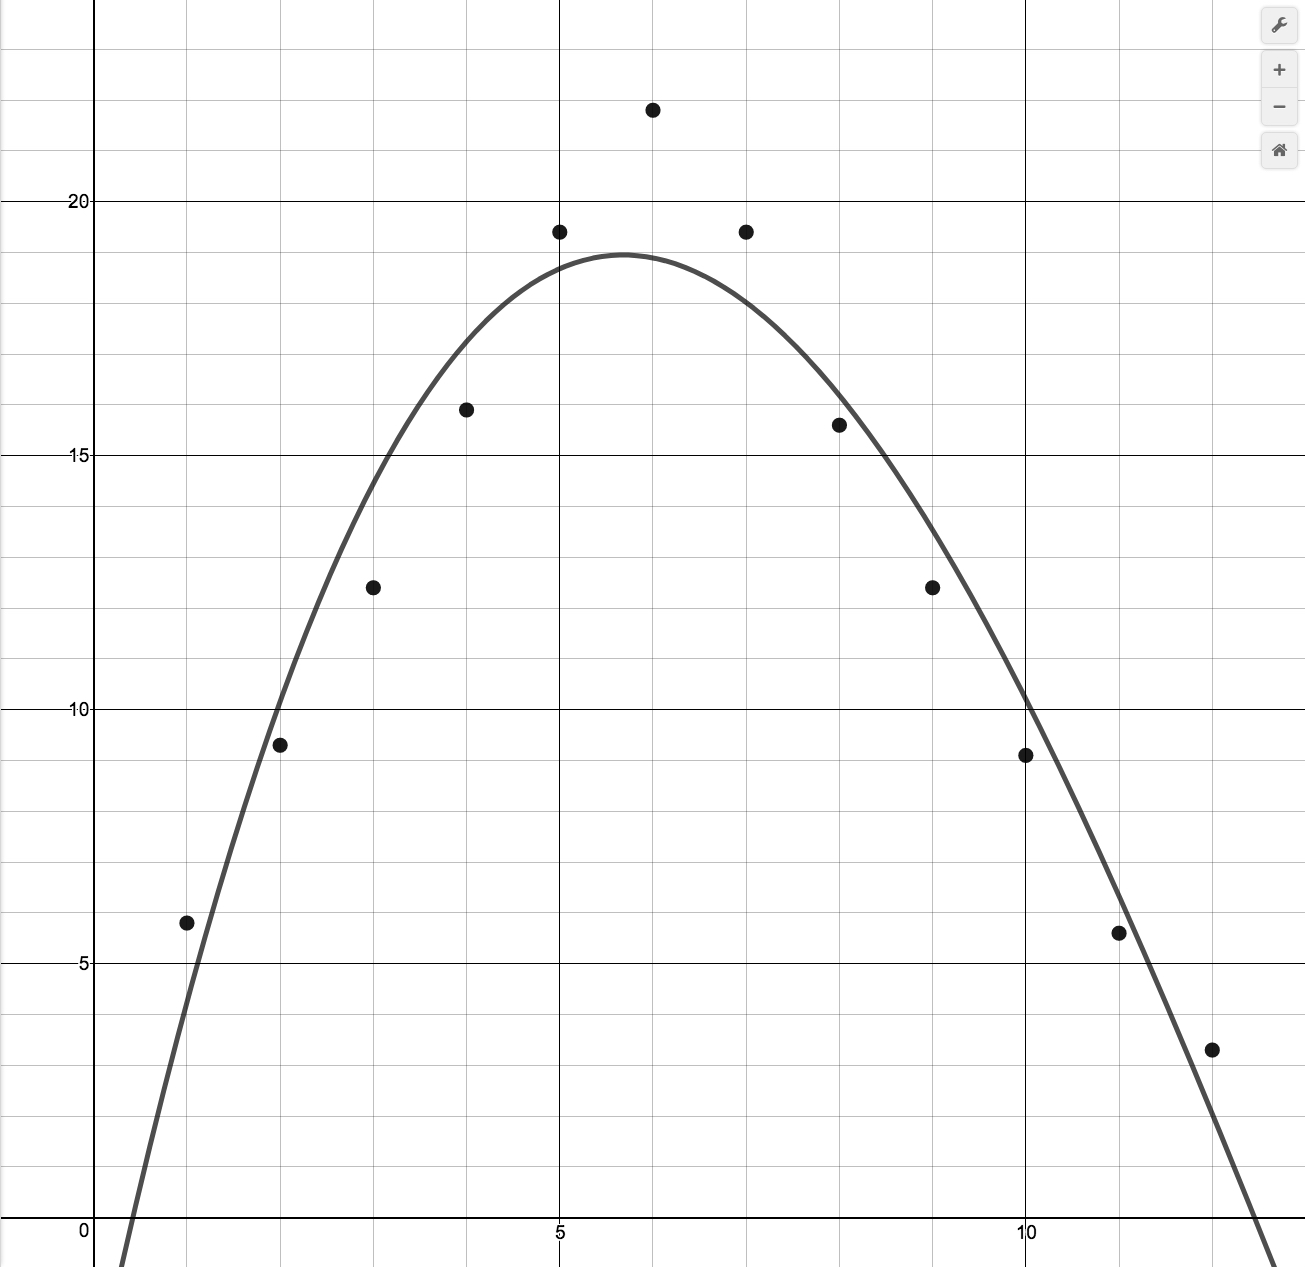
\includegraphics[width=2.5in]{./GraphsofPolynomialsGraphics/DaylightRegCubic.jpg} \hspace{.25in} & 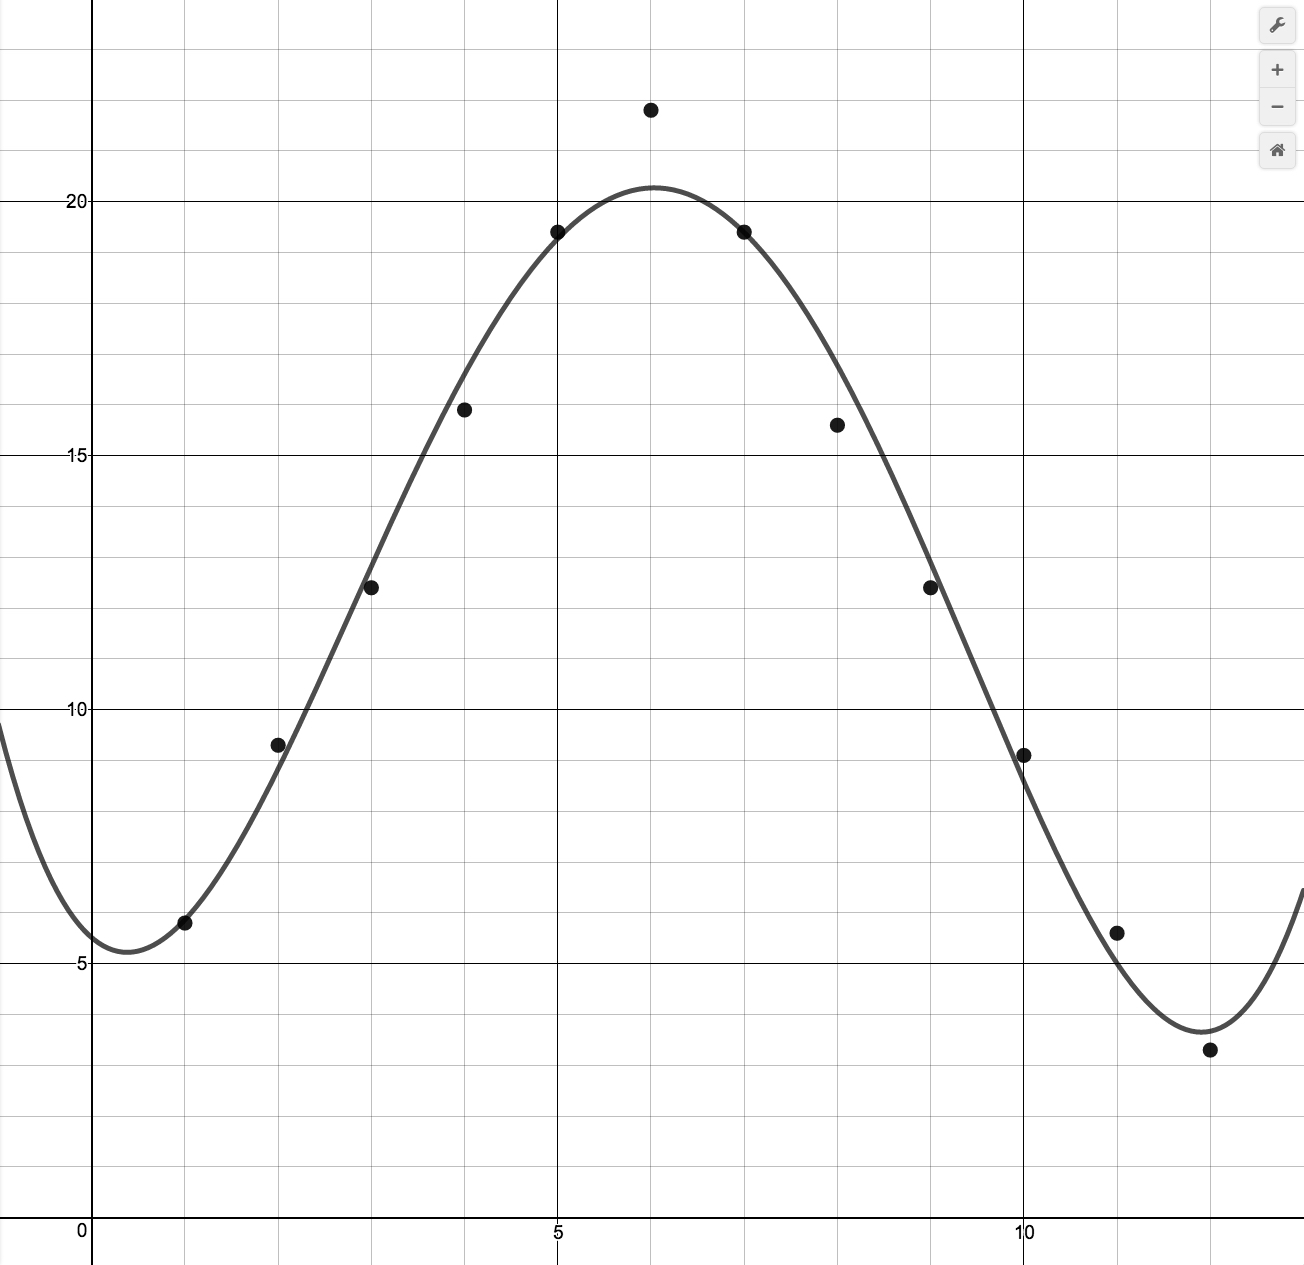
\includegraphics[width=2.5in]{./GraphsofPolynomialsGraphics/DaylightRegQuartic.jpg} \\

$y = p_{\mbox{\tiny $3$}}(x)$ \hspace{.25in} & $y = p_{\mbox{\tiny $4$}}(x)$ \\

\end{tabular}

\end{center}

\newpage

\item \begin{enumerate}

\item The scatter plot is shown below with each of the three regression models.

\item The quadratic model is $P_{\mbox{\tiny $2$}}(x) = -0.021x^{2} + 0.241x + 0.956$, $R^{2} = 0.7771$. \\
The cubic model is $P_{\mbox{\tiny $3$}}(x) = 0.005x^{3} - 0.103x^{2} + 0.602x + 0.573$,  $R^{2} = 0.9815$. \\
The quartic model is $P_{\mbox{\tiny $4$}}(x) = -0.000969x^{4} + 0.0253x^{3} - 0.240x^{2} + 0.944x + 0.330$,  $R^{2} = 0.9993$.

\item The models give maximums: $P_{\mbox{\tiny $2$}}(5.737) \approx 1.648$, $P_{\mbox{\tiny $3$}}(4.232) \approx 1.657$ and $P_{\mbox{\tiny $4$}}(3.784) \approx 1.630$.
\end{enumerate}



\hspace{-.1in} \begin{tabular}{ccc}

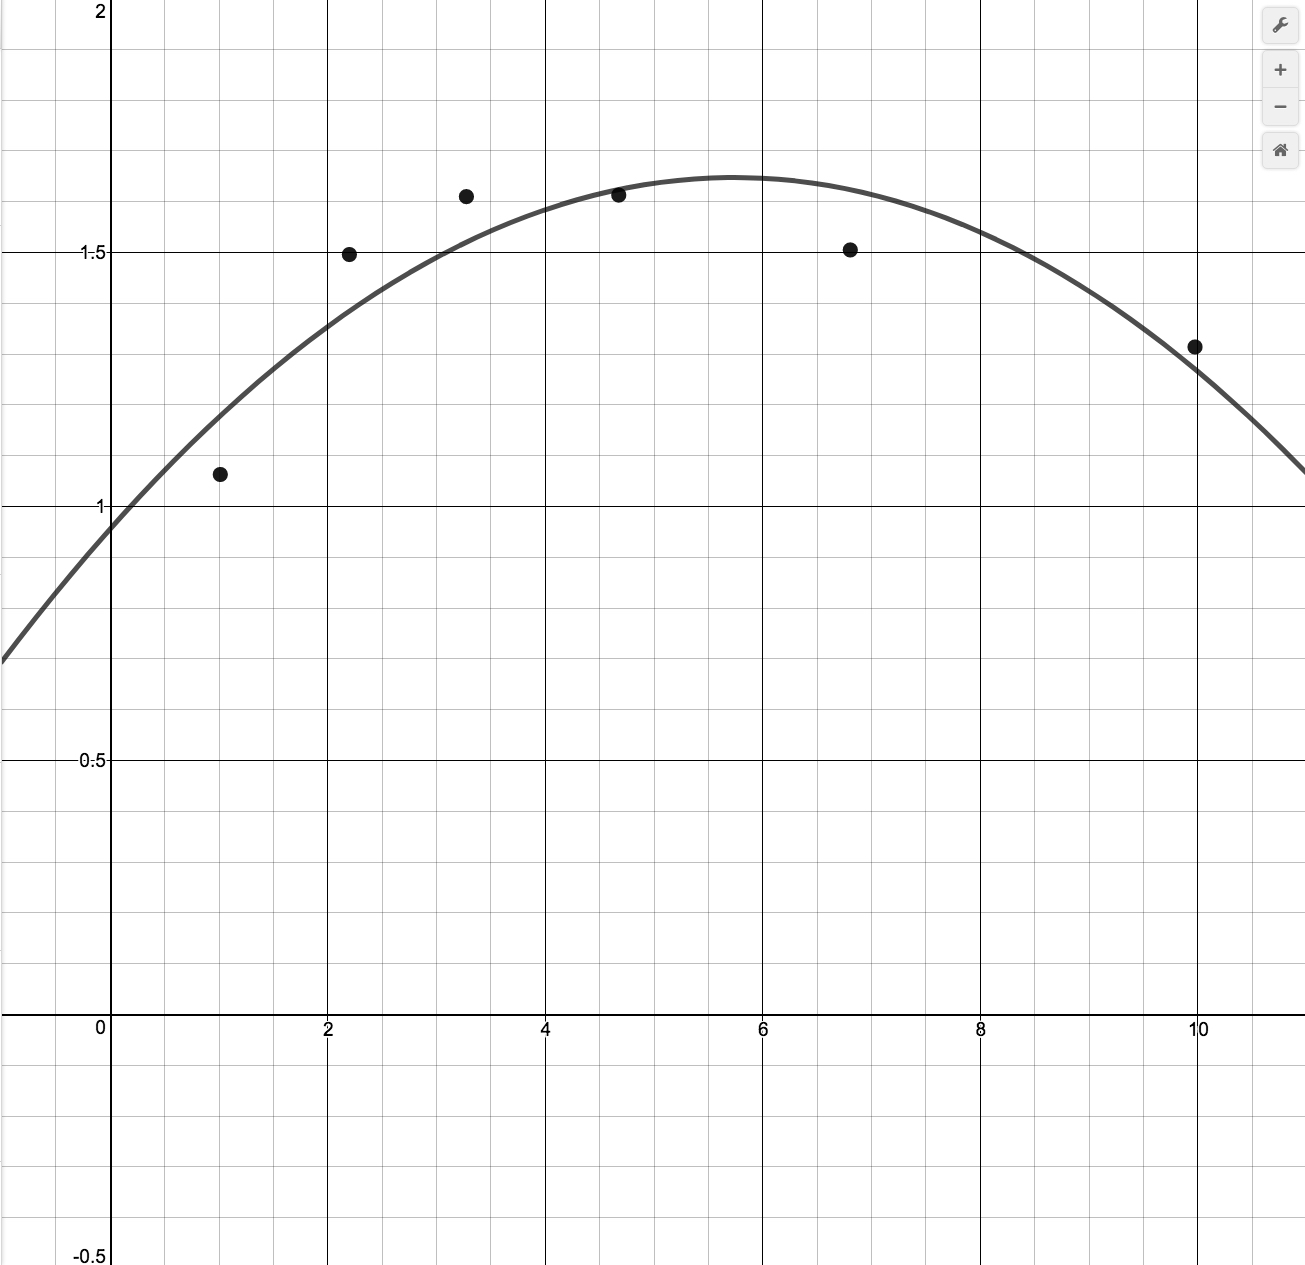
\includegraphics[width=1.8in]{./GraphsofPolynomialsGraphics/CircuitRegQuadratic.jpg} \hspace{.1in} &
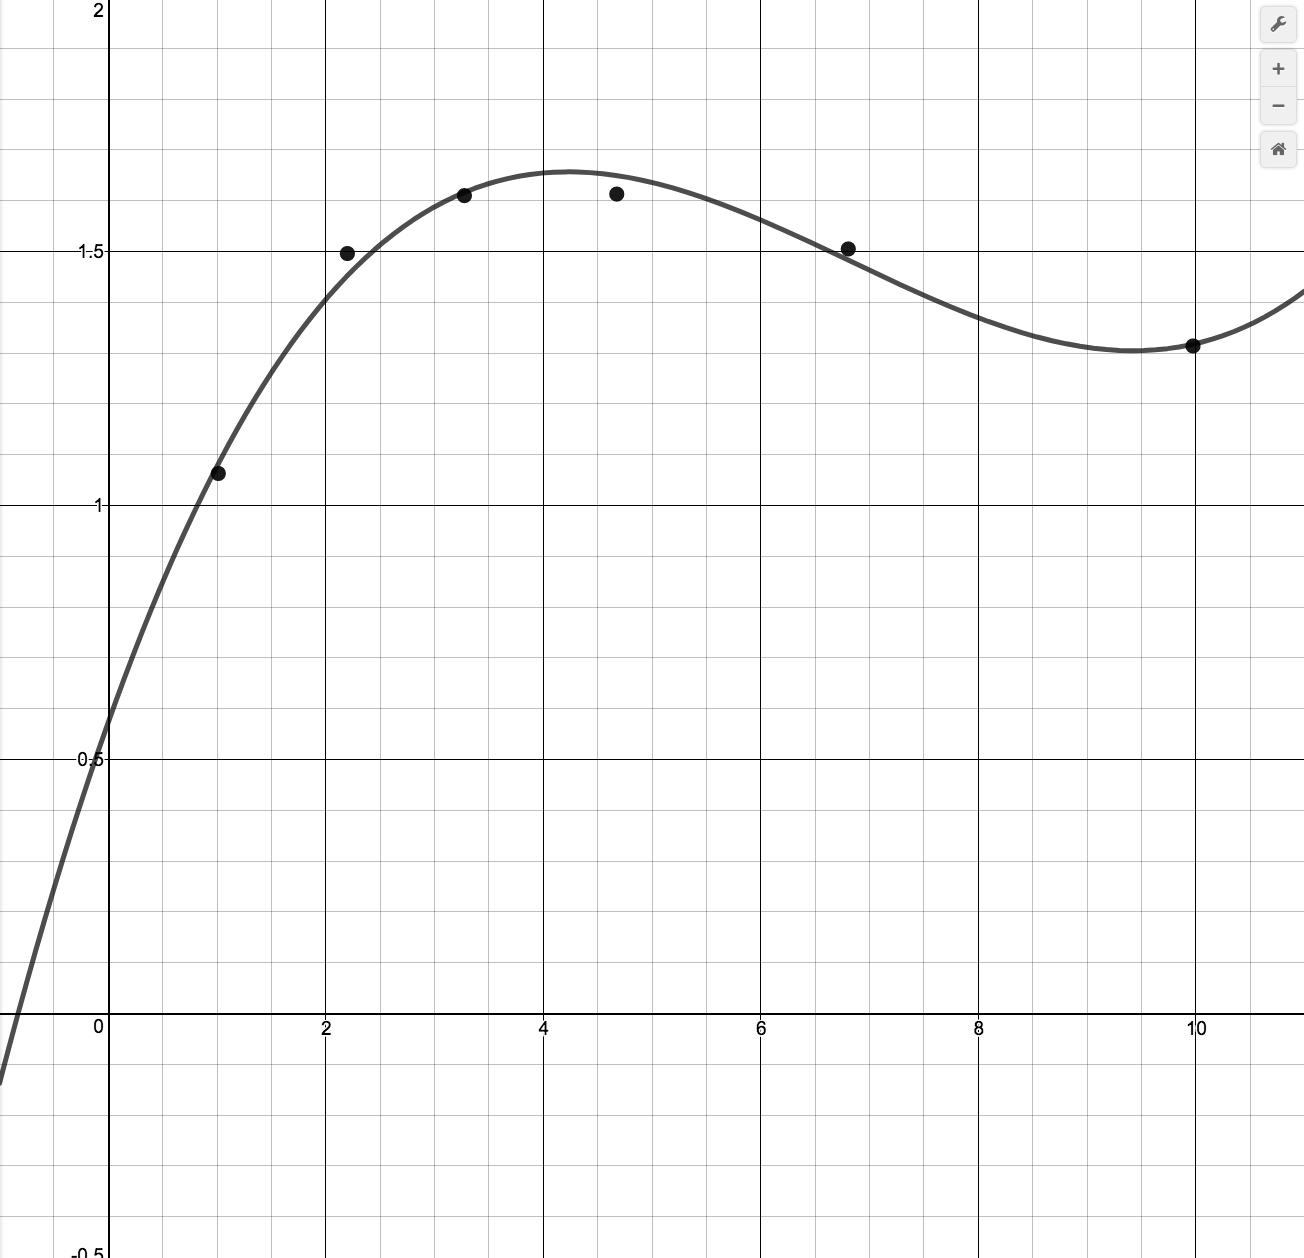
\includegraphics[width=1.8in]{./GraphsofPolynomialsGraphics/CircuitRegCubic.jpg} \hspace{.1in} &
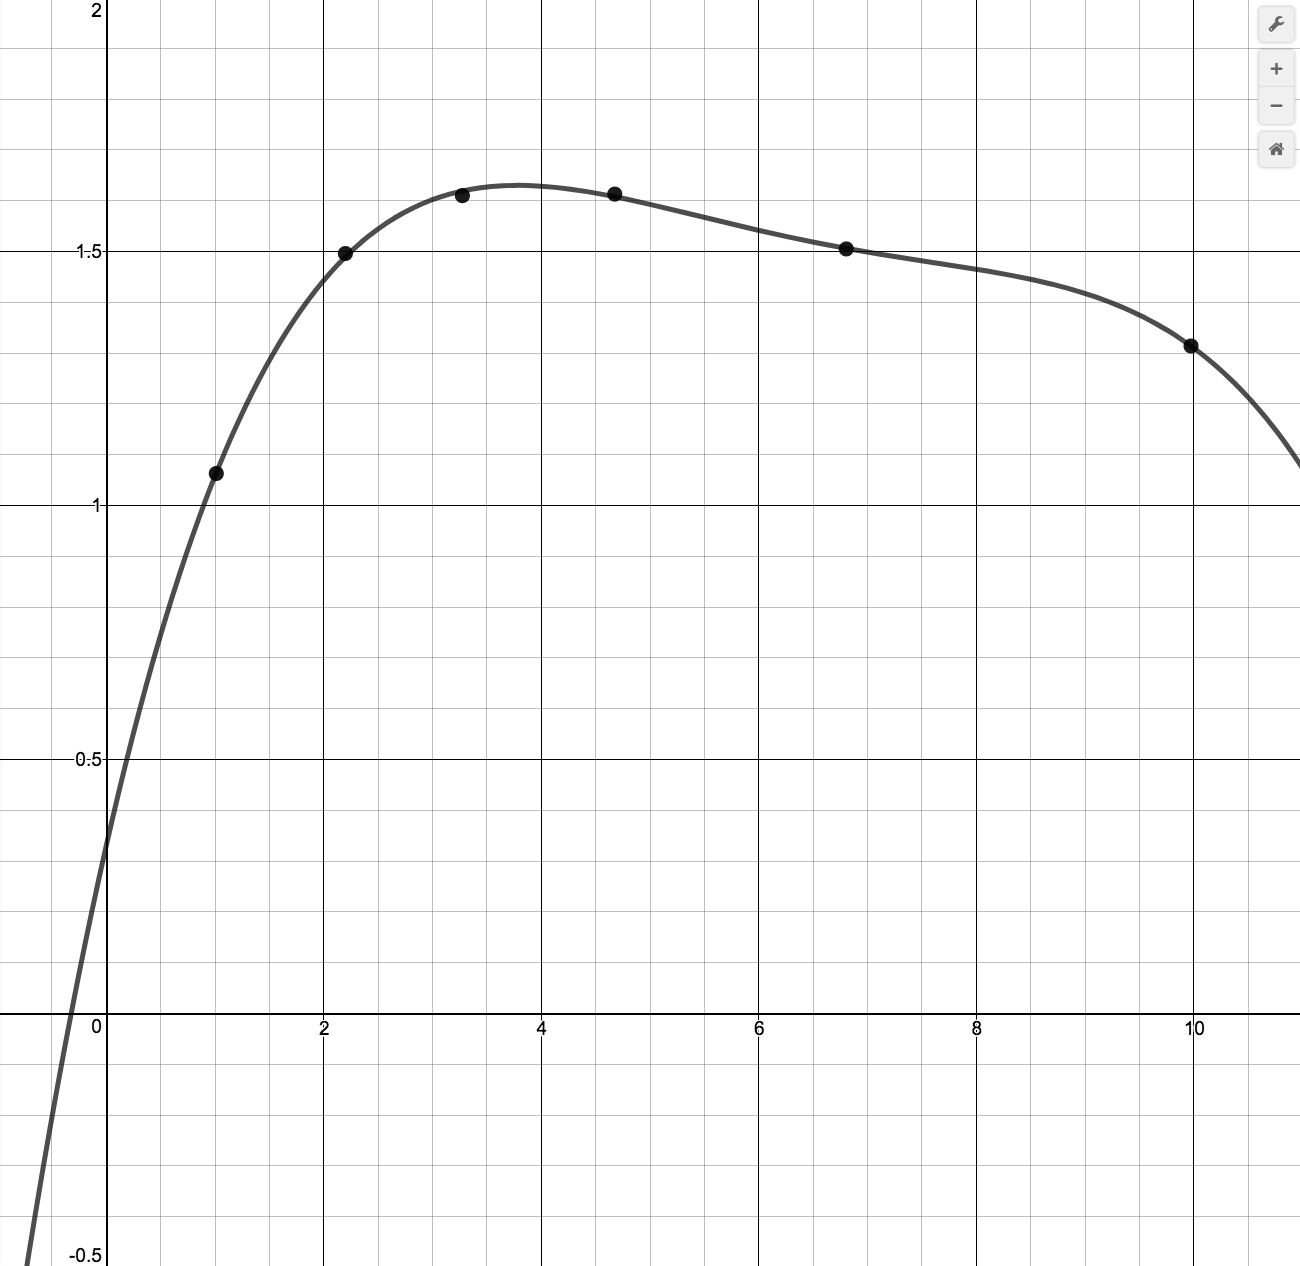
\includegraphics[width=1.8in]{./GraphsofPolynomialsGraphics/CircuitRegQuartic.jpg} \\

$y = P_{\mbox{\tiny $2$}}(x)$ \hspace{.1in} & $y = P_{\mbox{\tiny $3$}}(x)$ & $y = P_{\mbox{\tiny $4$}}(x)$\\

\end{tabular}

\item \begin{enumerate}

\item  as $x \rightarrow -\infty$, $p(x) \rightarrow -\infty$ and as $x \rightarrow \infty$, $p(x) \rightarrow -\infty$

\item The zeros appear to be: $x=-1.5$, even multiplicity - probably $2$ since it doesn't `look like' the graph is very flat near $x = 2$;  $x=0$, odd multiplicity - probably $1$ since the graph seems fairly linear as it passes through the origin;  $x=1$ odd multiplicity - probably $3$ or higher since the graph seems fairly `flat' near $x = 1$.

\item  local minimum:  approximately $(-0.773, -2.888)$;  local maximums:  approximately $(-1.5,0)$, and $(0.32, 0.532)$

\item  Based on the graph, even degree (at least $6$ based on multiplicities) with a negative leading coefficient based on the end behavior.

\item  We only have a \textit{portion} of the graph represented here.

\end{enumerate}

\addtocounter{enumi}{1}

\item We are looking for the largest open interval containing $x = -0.235$ for which the graph of $y = p(x)$ is at or above $y=-1.121$.  Since each of the gridlines on the $x$-axis correspond to $0.2$ units, we approximate this interval as  $(-1.25 \, \text{ish}, 1.1 \, \text{ish})$.

\addtocounter{enumi}{4}

\item 

\begin{multicols}{2}
\begin{enumerate} \addtocounter{enumii}{2} 
\item $L(x) = x^2$


\item $L(x) = x+1$

\end{enumerate}
\end{multicols}

\end{enumerate}


\closegraphsfile

\newpage

\section{The Remainder and Factor Theorems}

\mfpicnumber{1}

\opengraphsfile{Polydivision}

\setcounter{footnote}{0}

\label{Polydivision}


In Section \ref{GraphsofPolynomials} we saw how much of the `local' behavior of the graph of a polynomial function is  determined by the zeros of the polynomial function.  In that section, the polynomial functions we were given were mostly, if not completely, factored which greatly simplified the process for determining zeros.  In this section, we revisit the relationship between zeros and factors with the ultimate aim of taking a polynomial function given to us in the form stated in Definition \ref{polynomialfunction}  and determining its zeros. 

 We start by way of example:  suppose we wish to determine the zeros of  $f(x) = x^3 + 4x^2-5x-14$.  Setting $f(x)=0$ results in the polynomial equation $x^3 + 4x^2-5x-14=0$.   Despite all of the factoring techniques we learned (and forgot!) in Intermediate Algebra, this equation foils\footnote{pun intended} us at every turn. Knowing that the zeros of $f$ correspond to $x$-intercepts on the graph of $y=f(x)$, we use a graphing utility to produce the graph below on the left.  The graph suggests that the function has three zeros, one of which appears to be $x=2$ and two others for whom we are provided what we assume to be decimal approximations:  $x \approx -4.414$ and $x \approx -1.586$.    We can verify if these are zeros easily enough.   We find  $f(2) =(2)^2 + 4(2)^2-5(2)-14 = 0$,  but  $f(-4.414) \approx 0.0039$ and $f(-1.586) \approx 0.0022$,  While these last two values are probably by some measures,  `close' to $0$, they are not \textit{exactly} equal to $0$.  The question becomes:  is there a way to use the fact that $x=2$ is a zero to obtain the other two zeros?  Based on our experience, if $x=2$ is a zero, it seems that there should be a factor of $(x-2)$ lurking around in the factorization of $f(x)$.  In other words, we should expect that $x^3 + 4x^2-5x-14=(x-2) \, q(x)$, where $q(x)$ is some other polynomial.  How could we find such a $q(x)$, if it even exists?  The answer comes from our old friend, polynomial division. (See Section \ref{polylongdiv}.) Below on the right, we perform the long division:  $(x^3 + 4x^2-5x-14) \div (x-2)$ and obtain $x^2+6x+7$.
 
\begin{tabular}{m{4in}m{2.5in}}

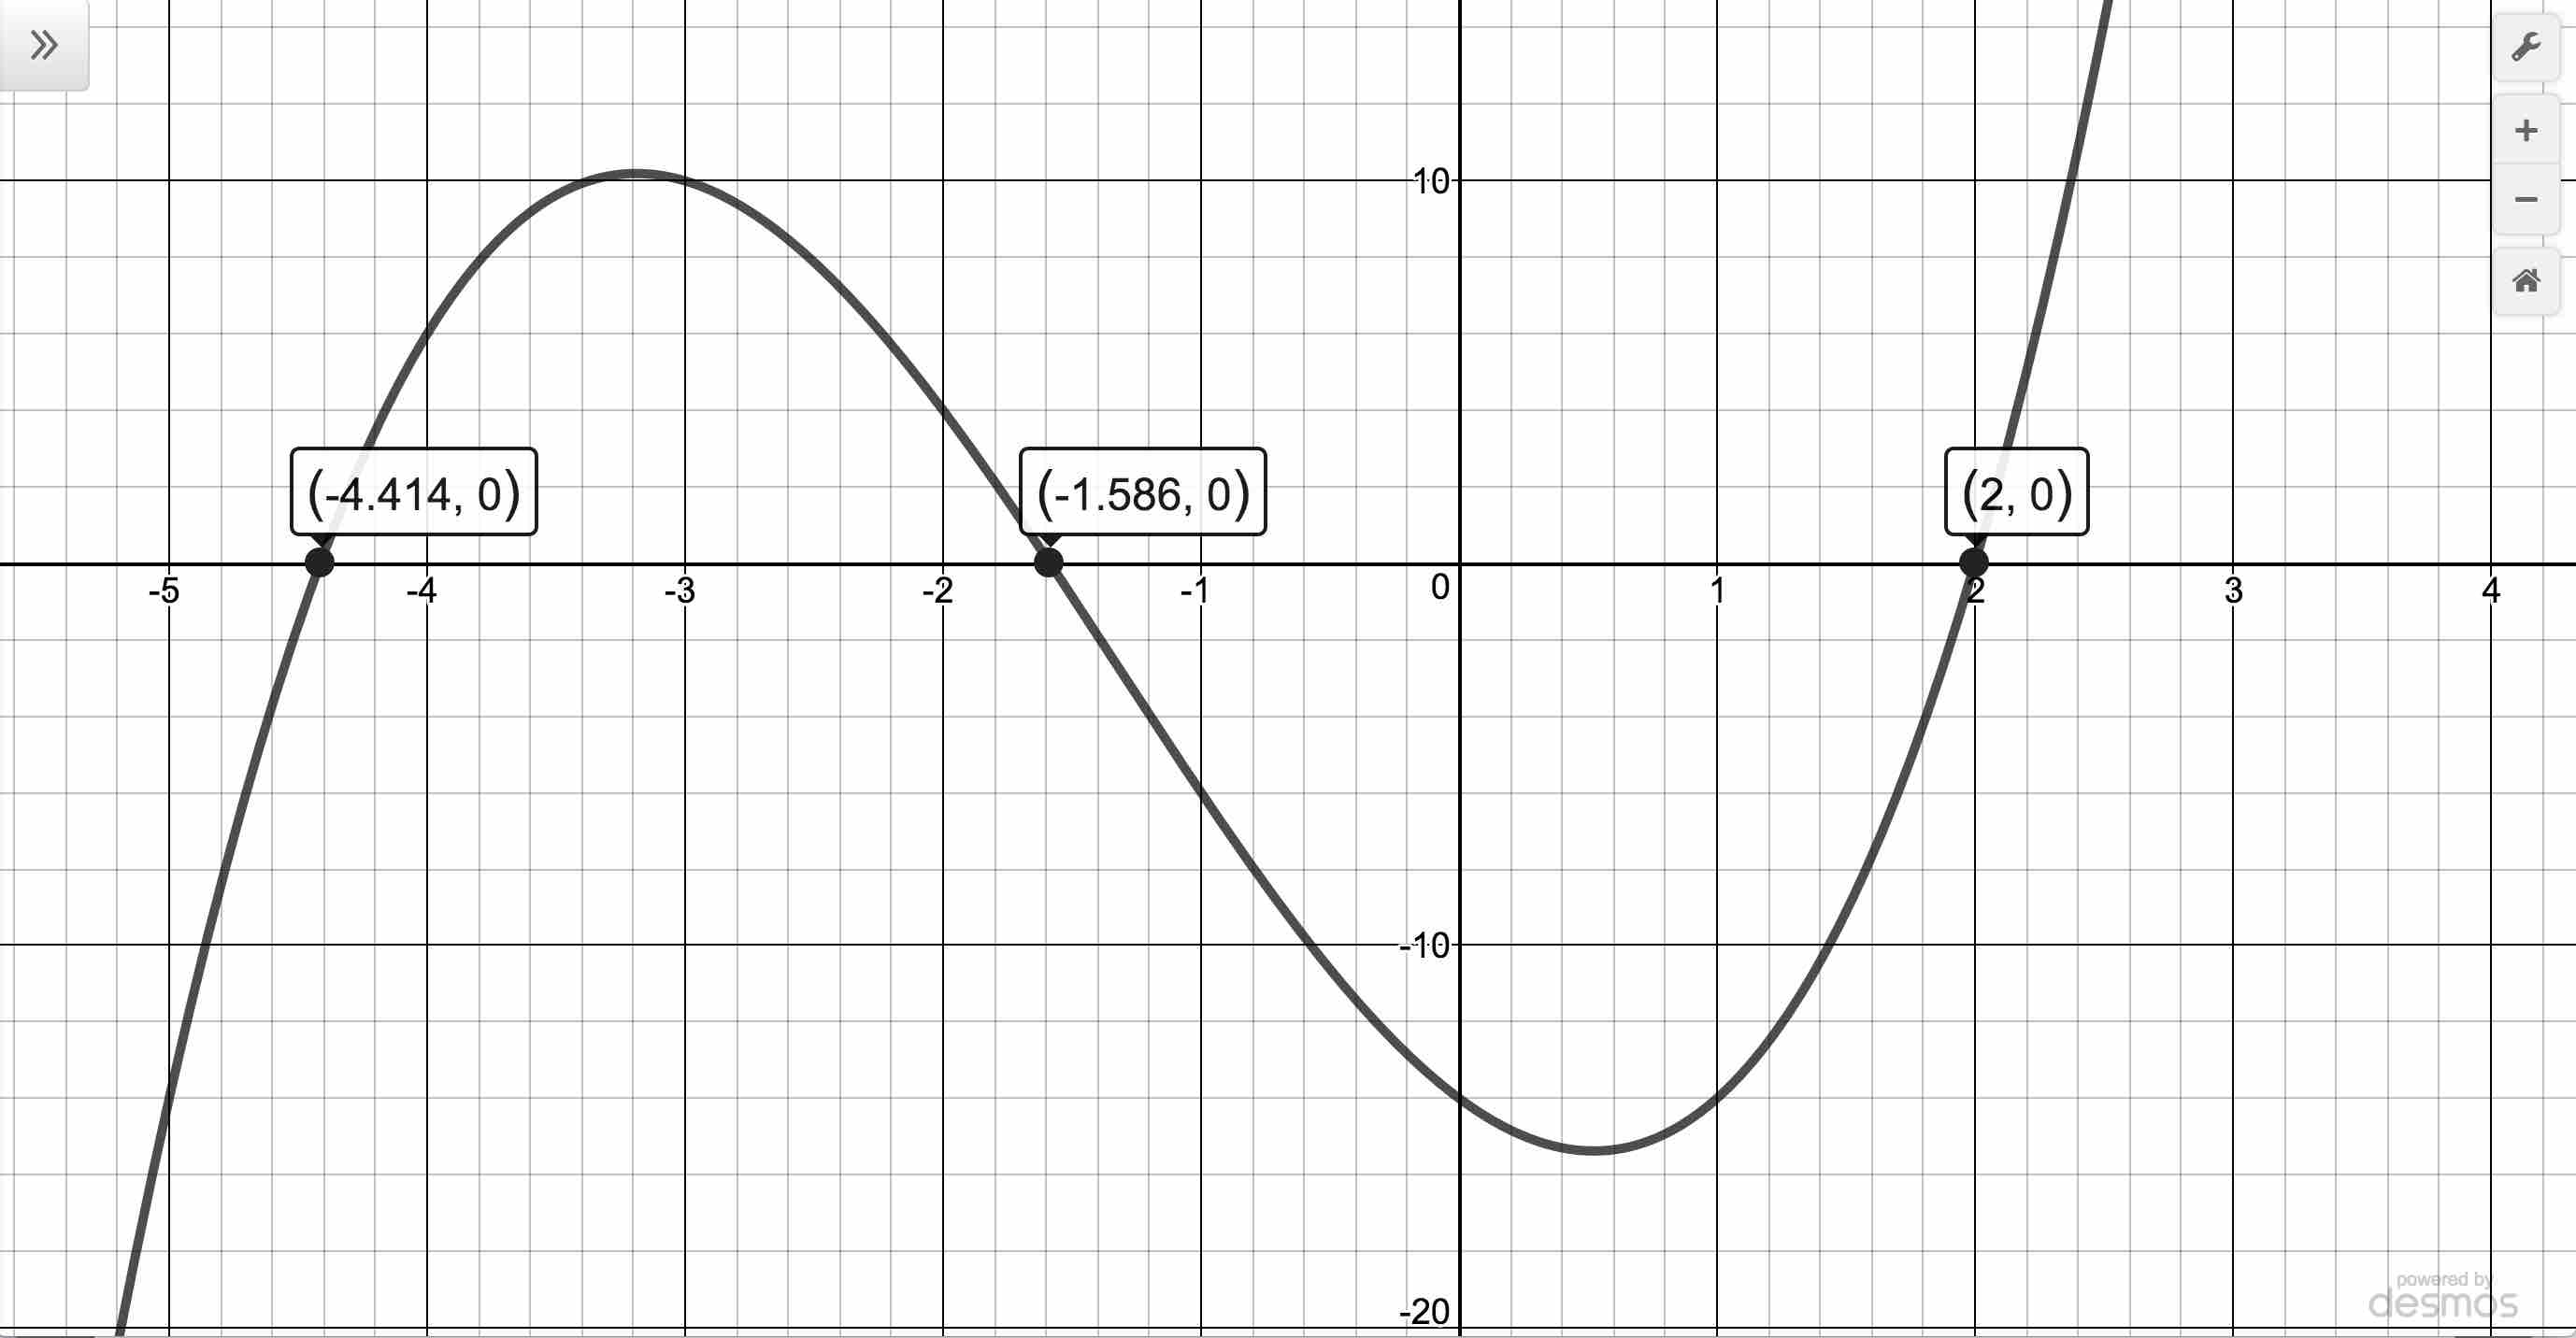
\includegraphics[height=2in]{./PolydivisionGraphics/PolyDiv01.jpg}

&

\setlength\arraycolsep{0.1pt}
\setlength\extrarowheight{2pt}

$\begin{array}{cccccccccc}

& & & & & x^2 & + & 6x & + & 7 \\ \hhline{~~~|-------}

x & - & 2 \, \vline& x^3 & + & 4x^2 & - & 5x & - & 14 \\

 &  &  -& \left(x^3 \right. & - & \left.  2x^2\right) &  &  &  &  \\ \hhline{~~~---~~~~} 
 &  &  &   &  & 6 x^2 & - & 5x &  &  \\ 
 &  &  &   & - & \left(6 x^2 \right. & - & \left. 12x \right) &  &  \\ \hhline{~~~~~---~~} 
 &  &  &   &   &  & & 7x  & - & 14 \\
 &  &  &   &   &  & - & \left( 7x \right. & - & \left. 14 \right) \\ \hhline{~~~~~~~---} 
 &   &  &  &  &  &  &  &  & 0
 
\end{array}$

\setlength\arraycolsep{5pt}
\setlength\extrarowheight{0pt}  \\

\end{tabular}



Said differently, $f(x) = x^3 + 4x^2-5x-14=(x-2)\left(x^2+6x+7\right)$.  Using this form of $f(x)$, we find the zeros by solving $(x-2)\left(x^2+6x+7\right)=0$.  Setting each factor equal to $0$, we get  $x-2=0$ (which gives us our known zero, $x=2$) as well as $x^2+6x+7=0$.   The latter doesn't factor nicely, so we apply the Quadratic Formula to get $x = -3 \pm \sqrt{2}$.  Sure enough, $-3 - \sqrt{2} \approx -4.414$ and $-3 +\sqrt{2} \approx -1.586$.  We leave it to the reader to show $f(-3-\sqrt{2}) = 0$ and $f(-3+\sqrt{2}) = 0$.  (See Exercise \ref{verifyrootsex}.) 

The point of this section is to generalize the technique applied here.  First up is a friendly reminder of what we can expect when we divide polynomials.

\smallskip

\colorbox{ResultColor}{\bbm

\begin{thm} \label{polydivthm} \textbf{Polynomial Division:} 

Suppose $d(x)$ and $p(x)$ are nonzero polynomial functions where the degree of $p$ is greater than or equal to the degree of $d$.  There exist two unique polynomial functions, $q(x)$ and $r(x)$, such that $p(x) = d(x) \, q(x) + r(x),\,$ where either $r(x) = 0$ or the degree of $r$ is strictly less than the degree of $d$.
\end{thm}
\ebm}

\smallskip

As you may recall, all of the polynomials in Theorem \ref{polydivthm} have special names.  The polynomial $p$ is called the \index{polynomial division ! dividend} \textbf{dividend}; $d$ is the \index{polynomial division ! divisor} \textbf{divisor}; $q$ is the \index{polynomial division ! quotient} \textbf{quotient}; $r$ is the \index{polynomial division ! remainder} \textbf{remainder}.  If $r(x)=0$ then $d$ is called a \index{polynomial division ! factor} \textbf{factor} of $p$.  The word `unique' here is critical in that it guarantees there is only \textit{one} quotient and remainder for each division problem.\footnote{Hence the use of the definite article `the' when speaking of \textit{the} quotient and \textit{the} remainder.} The proof of Theorem \ref{polydivthm} is usually relegated to a course in Abstract Algebra, but we can still use the result to establish two important facts which are the basis of the rest of the chapter.

\smallskip

\colorbox{ResultColor}{\bbm

\begin{thm} \label{remainderthm}\index{Remainder Theorem}\textbf{The Remainder Theorem:}  
Suppose $p$ is a polynomial function of degree at least $1$ and $c$ is a real number.  When $p(x)$ is divided by $x-c$ the remainder is $p(c)$.  Said differently, there is a polynomial  function $q(x)$ such that:  \[ p(x) = (x-c) q(x) + p(c)\]

\end{thm}
\ebm}

\smallskip


The proof of Theorem \ref{remainderthm} is a direct consequence of Theorem \ref{polydivthm}.  Since  $x-c$ has degree $1$, when a polynomial function is divided by $x-c$, the remainder is either $0$ or degree $0$ (i.e., a nonzero constant.)   In either case, $p(x) = (x-c) \, q(x) + r$, where $r$, the remainder, is a real number, possibly $0$.  It follows that $p(c) = (c-c) \, q(c) + r = 0 \cdot q(c) + r = r$, so we get $r = p(c)$ as required.  There is one last `low hanging fruit'\footnote{Jeff hates this expression and Carl included it just to annoy him.} to collect which we present below.

\smallskip

\colorbox{ResultColor}{\bbm

\begin{thm} \label{factorthm}\index{Factor Theorem}\textbf{The Factor Theorem:}  

Suppose $p$ is a nonzero polynomial function.  The real number $c$ is a zero of $p$ if and only if $(x-c)$ is a factor of $p(x)$.  

\end{thm}
\ebm}

\smallskip

Once again, we see the phrase `if and only if' which means there are really two things being said in  The Factor Theorem:  if $(x-c)$ is a factor of $p(x)$, then $c$ is a zero of $p$ and the \textit{only} way $c$ is a zero  of $p$ is if $(x-c)$ is a factor of $p(x)$.  We argue the Factor Theorem as follows:   if $(x-c)$ is a factor of $p(x)$, then $p(x) = (x-c) \, q(x)$ for some polynomial $q$.  Hence, $p(c) = (c-c) \, q(c) = 0$, so $c$ is a zero of $p$.  Conversely, suppose $c$ is a zero of $p$, so $p(c) = 0$.   The Remainder Theorem tells us $p(x) = (x-c)q(x) + p(c) = (x-c)q(x) + 0 = (x-c)q(x)$.   Hence, $(x-c)$ is a factor of $p(x)$. 

We have enough theory to explain why the concept of multiplicity (Definition \ref{multiplicity}) is well-defined. If $c$ is a zero of $p$, then The Factor Theorem tells us there is a polynomial function $q_{\text{\scriptsize $1$}}$ so that $p(x) = (x-c)q_{\text{\scriptsize $1$}}(x)$.  If $q_{\text{\scriptsize $1$}}(c) = 0$, then we apply the Factor Theorem to $q_{\text{\scriptsize $1$}}$ and find a  polynomial $q_{\text{\scriptsize $2$}}$ so that $q_{\text{\scriptsize $1$}}(x)  = (x-c) q_{\text{\scriptsize $2$}}(x)$.  Hence, we have  \[p(x) = (x-c) q_{\text{\scriptsize $1$}}(x) = (x-c) (x-c) q_{\text{\scriptsize $2$}}(x) = (x-c)^2 q_{\text{\scriptsize $2$}}(x).\]
We now `rinse and repeat' this process.  Since the degree of $p$ is a finite number, this process has to end at some point.  That is we arrive at a factorization  $p(x) = (x-c)^m q(x)$ where $q(c) \neq 0$. Suppose we arrive at a different factorization of $p$ using other methods.  That is, we find $p(x) = (x-c)^k Q(x)$, where $Q$ is a polynomial function with $Q(c) \neq 0$.   Then we have $(x-c)^m q(x) = (x-c)^k Q(x)$.  If $m \neq k$, then either $m<k$ or $m>k$.  Assuming the former, then we may divide both sides by $(x-c)^{m}$ to get: $q(x) = (x-c)^{k-m} Q(x)$.  Since $k>m$, $k-m>0$ and we would have $q(c) = (c-c)^{k-m} Q(c) = 0$, a contradiction since we are assuming $q(c) \neq 0$.  The assumption that $m>k$ likewise ends in a contradiction.  Therefore, we have $m = k$, so $p(x) = (x-c)^m q(x) = (x-c)^m Q(x)$.  By the uniqueness guaranteed in Theorem \ref{polydivthm}, we must have that $q(x) = Q(x)$.  Hence, we have shown the number $m$, as well as the quotient polynomial $q(x)$ are unique. The process outlined above, in which we coax out factors of $p(x)$ one at a time until we have all of them serves as a template for our work to come.


Of the things The Factor Theorem tells us, the most pragmatic is that we had better find a more efficient way to divide polynomial functions by quantities of the form $x-c$.  Fortunately, people like \href{http://en.wikipedia.org/wiki/Synthetic_division}{\underline{Ruffini}} and \href{http://en.wikipedia.org/wiki/Horner_scheme}{\underline{Horner}} have already blazed this trail.  Let's take a closer look at the long division we performed at the beginning of the section and try to streamline it.  First off, let's change all of the subtractions into additions by distributing through the $-1$s.


\setlength\arraycolsep{0.1pt}
\setlength\extrarowheight{2pt}

\[ \begin{array}{cccccccccc}

& & & & & x^2 & + & 6x & + & 7 \\ \hhline{~~~|-------}

x & - & 2 \, \vline& x^3 & + & 4x^2 & - & 5x & - & 14 \\

 &  &  &  -x^3  & + &   2x^2 &  &  &  &  \\ \hhline{~~~---~~~~} 
 &  &  &   &  & 6 x^2 & - & 5x &  &  \\ 
 &  &  &   & &-6 x^2  & + &  12x &  &  \\ \hhline{~~~~~---~~} 
 &  &  &   &   &  & & 7x  & - & 14 \\
 &  &  &   &   &  & & - 7x  & + &  14  \\ \hhline{~~~~~~~---} 
 &   &  &  &  &  &  &  &  & 0
 
\end{array}\]

\setlength\arraycolsep{5pt}
\setlength\extrarowheight{0pt}


Next, observe that the terms $-x^3$, $-6x^2$ and $-7x$ are the exact opposite of the terms above them.  The algorithm we use ensures this is always the case, so we can omit them without losing any information. Also note that the terms we `bring down' (namely the $-5x$ and $-14$) aren't really necessary to recopy, so we omit them, too.


\setlength\arraycolsep{0.1pt}
\setlength\extrarowheight{2pt}

\[ \begin{array}{cccccccccc}

& & & & & x^2 & + & 6x & + & 7 \\ \hhline{~~~|-------}

x & - & 2 \, \vline& \, \, x^3 & + & 4x^2 & - & 5x & - & 14 \\

 &  &  &   &  &   2x^2 &  &  &  &  \\ \hhline{~~~---~~~~} 
 &  &  &   &  & 6 x^2 &  &  &  &  \\ 
 &  &  &   & &  &  &  12x &  &  \\ \hhline{~~~~~---~~} 
 &  &  &   &   &  & & 7x  &  &  \\
 &  &  &   &   &  & &   &  &  14  \\ \hhline{~~~~~~~---} 
 &   &  &  &  &  &  &  &  & 0
 
\end{array}\]

\setlength\arraycolsep{5pt}
\setlength\extrarowheight{0pt}

Let's move terms up a bit and copy the $x^3$ into the last row.


\setlength\arraycolsep{0.1pt}
\setlength\extrarowheight{2pt}

\[ \begin{array}{cccccccccc}

& & & & & x^2 & + & 6x & + & 7 \\ \hhline{~~~|-------}

x & - & 2 \, \vline& \, \, x^3 & + & 4x^2 & - & 5x & - & 14 \\

 &  &  &   & &   2x^2 &  & 12x &  & 14 \\ \hhline{~~~-------} 
 &  &  & x^3  &  & 6 x^2 &  & 7x &  &0  \\  
\end{array}\]

\setlength\arraycolsep{5pt}
\setlength\extrarowheight{0pt}

Note that by arranging things in this manner, each term in the last row is obtained by adding the two terms above it.  Notice also that the quotient polynomial can be obtained by dividing each of the first three terms in the last row by $x$ and adding the results.   If you take the time to work back through the original division problem, you will find that this is exactly the way we determined the quotient polynomial.  This means that we no longer need to write the quotient polynomial down, nor the $x$ in the divisor, to determine our answer.

\setlength\arraycolsep{0.1pt}
\setlength\extrarowheight{2pt}

\[ \begin{array}{cccccccccc}


 & & - 2 \, \, \vline& \, \, x^3 & + & 4x^2 & - & 5x & - & 14 \\

 &  &  &   & &   2x^2 &  & 12x &  & 14 \\ \hhline{~~~-------} 
 &  &  & x^3  &  & 6 x^2 &  & 7x &  &0  \\  
\end{array}\]

\setlength\arraycolsep{5pt}
\setlength\extrarowheight{0pt}

We've streamlined things quite a bit so far, but we can still do more.  Let's take a moment to remind ourselves where the $2x^2$, $12x$ and $14$ came from in the second row.  Each of these terms was obtained by multiplying the terms in the quotient, $x^2$, $6x$ and $7$, respectively, by the $-2$ in $x-2$,  then by $-1$ when we changed the subtraction to addition.  Multiplying by $-2$ then by $-1$ is the same as multiplying by $2$, so we replace the $-2$ in the divisor by $2$.   Furthermore, the coefficients of the quotient polynomial match the coefficients of the first three terms in the last row, so we now take the plunge and write only the coefficients of the terms to get



\[ \begin{array}{rrrrr}


  2 \, \, \vline& 1 & 4 & -5  & -14 \\

   &&   2 &   12 &   14 \\ \hhline{~----} 
  & 1  &   6  &  7 &  0  \\  
\end{array}\]



We have constructed a \index{polynomial division ! synthetic division}\index{synthetic division tableau}\textbf{synthetic division tableau} for this polynomial division problem.  Let's re-work our division problem using this tableau to see how it greatly streamlines the division process.  To divide $x^3+4x^2-5x-14$ by $x-2$, we write $2$ in the place of the divisor and the coefficients of $x^3+4x^2-5x-14$ in for the dividend.  Then `bring down' the first coefficient of the dividend.

\bigskip

\begin{center}

\begin{tabular}{cc}

$ \begin{array}{rrrrr}


  2 \, \, \vline& 1 & 4 & -5  & -14 \\

   &  &    &    &  \\ \hhline{~----} 
  &   &     &   &    \\  
\end{array}$  \hspace{1in}
&


$ \begin{array}{rrrrr}


  2 \, \, \vline& 1 & 4 & -5  & -14 \\

   & \downarrow &    &    &  \\ \hhline{~----} 
  & 1  &     &   &    \\  
\end{array}$ \\

\end{tabular}

\end{center}

\bigskip

Next, take the $2$ from the divisor and multiply by the $1$ that was `brought down' to get $2$.  Write this underneath the $4$, then add to get $6$.

\bigskip

\begin{center}

\begin{tabular}{cc}

$ \begin{array}{rrrrr}


  2 \, \, \vline& 1 & 4 & -5  & -14 \\

   & \downarrow  &  2  &    &  \\ \hhline{~----} 
  & 1  &     &   &    \\  
\end{array}$ \hspace{1in}
&


$ \begin{array}{rrrrr}


  2 \, \, \vline& 1 & 4 & -5  & -14 \\

   & \downarrow &  2  &    &  \\ \hhline{~----} 
  & 1  &   6  &   &    \\  
\end{array}$ \\


\end{tabular}

\end{center}

\bigskip

Now take the $2$ from the divisor times the $6$ to get $12$, and add it to the $-5$ to get $7$.

\bigskip

\begin{center}

\begin{tabular}{cc}


$ \begin{array}{rrrrr}


  2 \, \, \vline& 1 & 4 & -5  & -14 \\

   & \downarrow &  2  &  12  &  \\ \hhline{~----} 
  & 1  &   6  &   &    \\  
\end{array}$ \hspace{1in}

&

$ \begin{array}{rrrrr}


  2 \, \, \vline& 1 & 4 & -5  & -14 \\

   & \downarrow &  2  &  12  &  \\ \hhline{~----} 
  & 1  &   6  & 7  &    \\  
\end{array}$ \\


\end{tabular}

\end{center}


Finally, take the $2$ in the divisor times the $7$ to get $14$, and add it to the $-14$ to get $0$.

\bigskip

\begin{center}

\begin{tabular}{cc}

$ \begin{array}{rrrrr}


  2 \, \, \vline& 1 & 4 & -5  & -14 \\

   & \downarrow &  2  &  12  & 14 \\ \hhline{~----} 
  & 1  &   6  & 7  &    \\  
\end{array}$ \hspace{1in} 

&

$ \begin{array}{rrrrr}


  2 \, \, \vline& 1 & 4 & -5  & -14 \\

   & \downarrow &  2  &  12  & 14 \\ \hhline{~----} 
  & 1  &   6  & 7  &  \fbox{$0$}  \\  
\end{array}$ \\



\end{tabular}

\end{center}

The first three numbers in the last row of our tableau are the coefficients of the quotient polynomial.  Remember, we started with a third degree polynomial and divided by a first degree polynomial, so the quotient is a second degree polynomial.  Hence the quotient is $x^2+6x+7$.  The number in the box is the remainder.  Synthetic division is our tool of choice for dividing polynomials by divisors of the form $x-c$.  It is important to note that it works \emph{only} for these kinds of divisors.\footnote{You'll need to use good old-fashioned polynomial long division for divisors of degree larger than 1.} Also take note that when a polynomial (of degree at least $1$) is divided by $x-c$, the result will be a polynomial of exactly one less degree. Finally, it is  worth the time to trace each step in synthetic division back to its corresponding step in long division.  While the authors have done their best to indicate where the algorithm comes from, there is no substitute for working through it yourself.

\begin{ex}  Use synthetic division to perform the following polynomial divisions.  Identify the quotient and remainder. Write the dividend, quotient and remainder in the form given in Theorem \ref{polydivthm}.

\begin{multicols}{3}
\begin{enumerate}

\item  $\left(5x^3 - 2x^2 + 1\right) \div (x-3)$ \vphantom{$\dfrac{4-8x-12x^2}{2x-3}$}
\item  $\left(t^3+8\right) \div (t+2)$ \vphantom{$\dfrac{4-8x-12x^2}{2x-3}$}
\item  $\dfrac{4-8z-12z^2}{2z-3}$

\end{enumerate}
\end{multicols}

{ \bf Solution.} 

\begin{enumerate}


\item When setting up the synthetic division tableau, the coefficients of even `missing' terms need to be accounted for, so we enter $0$ for the coefficient of $x$ in the dividend.  

\[ \begin{array}{rrrrr}


  3 \, \, \vline& 5 & -2 & 0  & 1 \\

   & \downarrow &  15  &  39  & 117 \\ \hhline{~----} 
  & 5  &   13  & 39  &  \fbox{$118$}  \\  
\end{array}\]

Since the dividend was a third degree polynomial function, the quotient is a second degree (quadratic) polynomial function with coefficients $5$, $13$ and $39$:   $q(x) = 5x^2+13x+39$. The remainder is $r(x) = 118$.  According to Theorem \ref{polydivthm}, we have $5x^3 - 2x^2 + 1 = (x-3)\left(5x^2+13x+39 \right) + 118$, which we leave to the reader to check.

\item  To use synthetic division here, we rewrite $t+2$ as $t-(-2)$ and proceed as before

\[ \begin{array}{rrrrr}


  -2 \, \, \vline& 1 & 0 & 0  & 8 \\

   & \downarrow &  -2  &  4  & -8 \\ \hhline{~----} 
  & 1  &   -2  & 4  &  \fbox{$0$}  \\  
\end{array}\]

We get the quotient $q(t) = t^2-2t+4$ and the remainder $r(t) =0$. Relating the dividend, quotient and remainder gives: $t^3+8 = (t+2)\left( t^2-2t+4 \right)$, which is a specific instance of the `sum of cubes' formula some of you may recall from Intermediate Algebra.  

\item To divide $4-8z-12z^2$ by $2z-3$, two things must be done.  First, we write the dividend in descending powers of $z$ as $-12z^2-8z+4$.  Second, since synthetic division works only for factors of the form $z-c$, we factor $2z-3$ as $2\left(z-\frac{3}{2}\right)$.  Hence, we are dividing  $-12z^2-8z+4$ by two factors:  $2$ and $\left(z-\frac{3}{2}\right)$.  Dividing first by $2$, we obtain $-6z^2-4z+2$.  Next, we divide  $-6z^2-4z+2$ by $\left(z-\frac{3}{2}\right)$:

\[ \begin{array}{rrrr}


  \frac{3}{2} \, \, \vline& -6 & -4 & 2   \\ [4pt]

   & \downarrow &  -9  & -\frac{39}{2}  \\ [4pt] \hhline{~---} 
  &  -6  &   -13  & \fbox{$-\frac{35}{2}$}  \\  
\end{array}\]


Hence,  $-6z^2-4z+2 = \left(z-\frac{3}{2}\right)(-6 z - 13) - \frac{35}{2}$.  However when it comes to writing  the dividend, quotient and remainder in the form given in Theorem \ref{polydivthm}, we need to find $q(z)$ and $r(z)$ so that  $-12z^2-8z+4 = (2z-3) q(z) + r(z)$. Hence, starting with $-6z^2-4z+2 = \left(z-\frac{3}{2}\right)(-6 z - 13) - \frac{35}{2}$, we multiply $2$ back on both sides:  

\[ \begin{array}{rcl}
 -6z^2-4z+2  & = & \left(z-\frac{3}{2}\right)(-6 z - 13) - \frac{35}{2}\\
 2\left(-6z^2-4z+2 \right) & = & 2 \left[ \left(z-\frac{3}{2}\right)(-6 z - 13) - \frac{35}{2} \right] \\
 -12z^2-8z+4 & = & 2 \left(z-\frac{3}{2}\right)(-6 z - 13) - 2 \left(\frac{35}{2} \right) \\
 -12z^2-8z+4 & = & (2z-3) (-6 z - 13) - 35  \\ \end{array} \]

 At this stage, we have written $-12z^2-8z+4$ in the \textbf{form} $(2z-3) q(z) + r(z)$, so we identify the quotient as  $q(z) = -6z-13$ and the remainder is $r(z) = -35$.  But how can we be sure these are the same quotient and remainder polynomial functions we would have obtained if we had taken the time to do the long division in the first place?   Because of the word   `unique' in Theorem \ref{polydivthm}.  The theorem states that there is only \textit{one} way to decompose $-12z^2-8z+4$ as $(2z-3)q(z) + r(z)$.  Since we have found such a way, we can be sure it is the only way.\footnote{But it wouldn't hurt to check, just this once.} \qed
\end{enumerate}

\end{ex}

The next example pulls together all of the concepts discussed in this section.  

\begin{ex} Let $p(x) = 2x^3-5x+3$.

\begin{enumerate}

\item  Find $p(-2)$ using The Remainder Theorem.  Check your answer by substitution.

\item  Verify  $x=1$ is a zero of $p$ and use this information to all the real zeros of $p$.

\end{enumerate}

{\bf Solution.}

\begin{enumerate}

\item  The Remainder Theorem states $p(-2)$ is the remainder when $p(x)$ is divided by $x-(-2)$.  We set up our synthetic division tableau below.  We are careful to record the coefficient of $x^2$ as $0$:

\[\begin{array}{rrrrr}
 -2 \, \, \vline& 2 & 0 & -5  & 3 \\

   & \downarrow &  -4  &  8  & -6 \\ \hhline{~----} 
  & 2  &   -4  & 3 &  \fbox{$-3$}  \\  
\end{array}\]

According to the Remainder Theorem, $p(-2) = -3$.  We can check this by direct substitution into the formula for $p(x)$:  $p(-2) = 2(-2)^3-5(-2)+3 = -16+10+3=-3$.

\item We verify $x=1$ is a zero of $p$ by evaluating $p(1) = 2(1)^3-5(1)+3 = 0$.  To see if there are any more real zeros, we need to solve $p(x) = 2x^3-5x+3 = 0$.  From the Factor Theorem, we know since $p(1) = 0$,  we can factor $p(x)$ as $(x-1)q(x)$.  To find $q(x)$, we use synthetic division:

\[\begin{array}{rrrrr}
 1 \, \, \vline& 2 & 0 & -5  & 3 \\

   & \downarrow &  2  &  2  & -3 \\ \hhline{~----} 
  & 2  &   2  & -3 &  \fbox{$0$}  \\  
\end{array}\]

As promised, our remainder is $0$, and we get  $p(x) = (x-1)\left( 2x^2 + 2x - 3\right)$.  Setting this form of $p(x)$ equal to  $0$ we get $(x-1)\left( 2x^2 + 2x - 3\right) = 0$.  We recover  $x = 1$ from setting $x-1=0$  but we also obtain $x = \frac{-1 \pm \sqrt{7}}{2}$ from  $2x^2 + 2x - 3=0$, courtesy of the Quadratic Formula.   \qed
\end{enumerate}
\end{ex}

Our next example demonstrates how we can extend the synthetic division tableau to accommodate zeros of multiplicity greater than $1$.

\begin{ex}  Let $p(x) = 4x^4-4x^3-11x^2+12x-3$. Show $x=\frac{1}{2}$ is a zero of multiplicity $2$ and find all of the remaining real zeros of $p$.


{\bf Solution.}  While computing $p\left(\frac{1}{2} \right) = 0$ shows $x=\frac{1}{2}$  is a zero of $p$, to prove it has multiplicity $2$, we need to factor $p(x) = \left(x - \frac{1}{2}\right)^2 q(x)$ with $q\left( \frac{1}{2} \right) \neq 0$,.   We set up for synthetic division, but instead of stopping after the first division, we continue the tableau downwards and divide $\left(x - \frac{1}{2}\right)$ directly into the quotient we obtained from the first division as follows:

\[\begin{array}{rrrrrr}
 \frac{1}{2} \, \, \vline& 4 & -4 & -11  & 12 & -3 \\

   & \downarrow &  2  &  -1  & -6 & 3\\ \hhline{~-----} 
   
  \frac{1}{2} \, \, \vline&  4  &   -2  & -12 & 6 &  \fbox{$0$}  \\
    
      & \downarrow &  2  &  0  & -6 &\\ \hhline{~----} 
      
       & 4  &   0  & -12 & \fbox{0} &   \\  



\end{array}\]

We get:\footnote{For those wanting more detail:  the first division gives:  $4x^4-4x^3-11x^2+12x-3=\left(x-\frac{1}{2}\right) \left(4x^3-2x^2-12x+6\right)$.  The second division gives: $4x^3-2x^2-12x+6=\left(x-\frac{1}{2}\right)\left(4x^2-12\right)$.}   $4x^4-4x^3-11x^2+12x-3 = \left(x-\frac{1}{2}\right)^2\left(4x^2-12\right)$.  Note if we let $q(x) = 4x^2-12$, then $q\left(\frac{1}{2} \right) = 4\left(\frac{1}{2} \right)^2 - 12 = -11 \neq 0$  which proves $x = \frac{1}{2}$ is a zero of $p$ of multiplicity $2$.   To find the remaining zeros of $p$, we set the quotient $4x^2-12=0$, so $x^2 = 3$ and extract square roots to get $x = \pm \sqrt{3}$.  \qed

\end{ex}

A couple of things about the last example are worth mentioning. First, the extension of the synthetic division tableau for repeated divisions will be a common site in the sections to come. Typically, we will start with a higher order polynomial and peel off one zero at a time until we are left with a quadratic, whose roots can always be found using the Quadratic Formula.  Secondly, we found $x = \pm \sqrt{3}$ are zeros of $p$.  The Factor Theorem guarantees $\left(x-\sqrt{3}\right)$ and $\left(x - \left(-\sqrt{3}\right)\right)$ are both factors of $p$.  We can certainly put the Factor Theorem to the test and continue the synthetic division tableau from above to see what happens.

\[\begin{array}{rrrrrr}
 \frac{1}{2} \, \, \vline& 4 & -4 & -11  & 12 & -3 \\

  & \downarrow &  2  &  -1  & -6 & 3\\ \hhline{~-----} 
  
  \frac{1}{2} \, \, \vline&  4  &   -2  & -12 & 6 &  \fbox{$0$}  \\
    
  & \downarrow &  2  &  0  & -6 &\\ \hhline{~----} 
 
  
 \sqrt{3} \, \, \vline  & 4  &   0  & -12 & \fbox{0} &   \\
  
                        & \downarrow &  4\sqrt{3}  & 12  & &\\ \hhline{~---} 
 
   -\sqrt{3} \, \, \vline  & 4  &  4\sqrt{3}  & \fbox{0} &  &   \\  
       
                          & \downarrow &  -4\sqrt{3}  &   & &\\ \hhline{~--} 
       
													& 4  &  \fbox{0}  &  &  &   \\

\end{array}\]

This gives us

 \[\begin{array}{rcl} 
 
 p(x) & = &  4x^4-4x^3-11x^2+12x-3 \\
        & = & \left(x-\frac{1}{2}\right)^2 \left(x-\sqrt{3}\right)\left(x - \left(-\sqrt{3}\right)\right) (4) \\
        & = &  4\left(x-\frac{1}{2}\right)^2 \left(x-\sqrt{3}\right)\left(x - \left(-\sqrt{3}\right)\right) \\ \end{array} \]

We have shown that $p$ is a product of its leading coefficient times linear factors of the form $(x-c)$ where $c$ are zeros of $p$. It may surprise and delight the reader that, in theory, all polynomials can be reduced to this kind of factorization.  We leave that discussion to Section \ref{ComplexZeros}, because the zeros may not be real numbers.  Our final theorem in the section gives us an upper bound on the number of real zeros. 

\medskip

\colorbox{ResultColor}{\bbm
\begin{thm}  \label{nzerosreal} 

Suppose $f$ is a polynomial of degree $n \geq 1$.  Then $f$ has at most $n$ real zeros, counting multiplicities.

\end{thm}
\ebm}

\medskip

Theorem \ref{nzerosreal} is a consequence of the Factor Theorem and polynomial multiplication.  Every zero $c$ of $f$ gives us a factor of the form $(x-c)$ for $f(x)$.  Since $f$ has degree $n$, there can be at most $n$ of these factors.  The next section provides us some tools which not only help us determine where the real zeros are to be found, but which real numbers they may be.

\medskip

We close this section with a summary of several concepts previously presented.  You should take the time to look back through the text to see where each concept was first introduced and where each connection to the other concepts was made.

\medskip

\colorbox{ResultColor}{\bbm

\centerline{\textbf{Connections Between Zeros, Factors and Graphs of Polynomial Functions}}

\medskip

\hspace{.17in} Suppose $p$ is a polynomial function of degree $n \geq 1$.  The following statements are equivalent:

\begin{itemize}

\item The real number $c$ is a zero of $p$
\item $p(c) = 0$
\item $x = c$ is a solution to the polynomial equation $p(x) = 0$
\item $(x - c)$ is a factor of $p(x)$
\item The point $(c, 0)$ is an $x$-intercept of the graph of $y = p(x)$

\end{itemize}

\ebm}

\newpage

\subsection{Exercises}


In Exercises \ref{synthdivreviewfirst} - \ref{synthdivreviewlast}, use synthetic division to perform the following polynomial divisions.  Identify the quotient and remainder. Write the dividend, quotient and remainder in the form given in Theorem \ref{polydivthm}.

\begin{multicols}{2}
\begin{enumerate}


\item $\left(3x^2-2x+1 \right) \div \left(x-1\right)$ \label{synthdivreviewfirst}
\item $\left(x^2-5 \right) \div \left(x-5\right)$

\setcounter{HW}{\value{enumi}}
\end{enumerate}
\end{multicols}

\begin{multicols}{2}
\begin{enumerate}
\setcounter{enumi}{\value{HW}}

\item $\left(3-4t-2t^2 \right) \div \left(t+1\right)$
\item $\left(4t^2-5t +3\right) \div \left(t+3\right)$

\setcounter{HW}{\value{enumi}}
\end{enumerate}
\end{multicols}

\begin{multicols}{2}
\begin{enumerate}
\setcounter{enumi}{\value{HW}}

\item $\left(z^3 + 8 \right) \div \left(z+2\right)$
\item $\left(4z^3 +2z-3 \right) \div \left(z -3\right)$

\setcounter{HW}{\value{enumi}}
\end{enumerate}
\end{multicols}

\begin{multicols}{2}
\begin{enumerate}
\setcounter{enumi}{\value{HW}}

\item $\left(18x^2-15x-25\right) \div \left(x - \frac{5}{3} \right)$
\item $\left(4x^2-1 \right) \div \left(x - \frac{1}{2} \right)$

\setcounter{HW}{\value{enumi}}
\end{enumerate}
\end{multicols}

\begin{multicols}{2}
\begin{enumerate}
\setcounter{enumi}{\value{HW}}

\item $\left(2t^3+t^2+2t+1 \right) \div \left(t + \frac{1}{2} \right)$
\item $\left(3t^3 - t + 4 \right) \div \left(t - \frac{2}{3} \right)$

\setcounter{HW}{\value{enumi}}
\end{enumerate}
\end{multicols}

\begin{multicols}{2}
\begin{enumerate}
\setcounter{enumi}{\value{HW}}

\item $\left(2z^3 - 3z +1 \right) \div \left(z - \frac{1}{2} \right)$
\item $\left(4z^4-12z^3+13z^2 -12z+9\right) \div \left(z - \frac{3}{2} \right)$

\setcounter{HW}{\value{enumi}}
\end{enumerate}
\end{multicols}

\begin{multicols}{2}
\begin{enumerate}
\setcounter{enumi}{\value{HW}}

\item $\left(x^4-6x^2+9 \right) \div \left(x -\sqrt{3} \right)$
\item $\left(x^6-6x^4+12x^2-8\right) \div \left(x +\sqrt{2} \right)$ \label{synthdivreviewlast}

\setcounter{HW}{\value{enumi}}
\end{enumerate}
\end{multicols}

In Exercises \ref{remainderexerfirst} - \ref{remainderexerlast}, find $p(c)$ using the Remainder Theorem.  If $p(c) = 0$, use the Factor Theorem to partially factor the polynomial function.

\begin{multicols}{2}
\begin{enumerate}
\setcounter{enumi}{\value{HW}}

\item $p(x) = 2x^2 - x + 1$, $c = 4$ \label{remainderexerfirst}
\item $p(x) = 4x^2-33x-180$, $c = 12$

\setcounter{HW}{\value{enumi}}
\end{enumerate}
\end{multicols}


\begin{multicols}{2}
\begin{enumerate}
\setcounter{enumi}{\value{HW}}

\item $p(t) = 2t^3 - t + 6$, $c=-3$
\item $p(t) = t^3+2t^2+3t+4$, $c =-1$

\setcounter{HW}{\value{enumi}}
\end{enumerate}
\end{multicols}

\begin{multicols}{2}
\begin{enumerate}
\setcounter{enumi}{\value{HW}}

\item $p(z) =3z^3-6z^2+4z-8$, $c=2$
\item $p(z) = 8z^3+12z^2+6z+1$, $c =-\frac{1}{2}$

\setcounter{HW}{\value{enumi}}
\end{enumerate}
\end{multicols}

\begin{multicols}{2}
\begin{enumerate}
\setcounter{enumi}{\value{HW}}

\item $p(x) = x^4 - 2x^2+4$, $c=\frac{3}{2}$
\item $p(x) = 6x^4-x^2+2$, $c =-\frac{2}{3}$

\setcounter{HW}{\value{enumi}}
\end{enumerate}
\end{multicols}


\begin{multicols}{2}
\begin{enumerate}
\setcounter{enumi}{\value{HW}}

\item $p(t) = t^4 +t^3-6t^2-7t-7$, $c=-\sqrt{7}$
\item $p(t) = t^2-4t+1$, $c =2-\sqrt{3}$ \label{remainderexerlast}

\setcounter{HW}{\value{enumi}}
\end{enumerate}
\end{multicols}



In Exercises \ref{factorpolyzerofirst} - \ref{factorpolyzerolast}, you are given a polynomial function and one of its zeros.  Find the remaining real zeros and factor the polynomial.  

\begin{multicols}{2}
\begin{enumerate}
\setcounter{enumi}{\value{HW}}

\item $x^{3} - 6x^{2} + 11x - 6, \;\; c = 1$ \label{factorpolyzerofirst}
\item $x^{3} - 24x^{2} + 192x - 512, \;\; c = 8$

\setcounter{HW}{\value{enumi}}
\end{enumerate}
\end{multicols}

\begin{multicols}{2}
\begin{enumerate}
\setcounter{enumi}{\value{HW}}

\item $3t^{3} + 4t^{2} - t - 2, \;\; c = \frac{2}{3}$
\item $2t^3-3t^2-11t+6, \;\; c=\frac{1}{2}$

\setcounter{HW}{\value{enumi}}
\end{enumerate}
\end{multicols}

\begin{multicols}{2}
\begin{enumerate}
\setcounter{enumi}{\value{HW}}

\item $z^3+2z^2-3z-6, \;\; c = -2$
\item $2z^3-z^2-10z+5, \;\; c=\frac{1}{2}$

\setcounter{HW}{\value{enumi}}
\end{enumerate}
\end{multicols}

\vspace*{-0.2in}
\enlargethispage{0.2in}
\begin{enumerate}
\setcounter{enumi}{\value{HW}}

\item $4x^{4} - 28x^{3} + 61x^{2} - 42x + 9$, $c = \frac{1}{2}$ is a zero of multiplicity 2 

\item  $t^5+2t^4-12t^3-38t^2-37t-12$, $c=-1$ is a zero of multiplicity 3

\item $125z^{5} - 275z^{4} - 2265z^{3} - 3213z^{2} - 1728z - 324$, $c = -\frac{3}{5}$ is a zero of multiplicity 3

\item $x^{2} - 2x - 2, \;\; c = 1 - \sqrt{3}$ \label{factorpolyzerolast}

\setcounter{HW}{\value{enumi}}
\end{enumerate}


\begin{enumerate}
\setcounter{enumi}{\value{HW}}

\item Find a quadratic polynomial with \underline{integer} coefficients which has $x = \dfrac{3}{5} \pm \dfrac{\sqrt{29}}{5}$ as its real zeros.

\item  \label{verifyrootsex}  For $f(x) = x^3 + 4x^2-5x-14$, show $f(-3-\sqrt{2}) = 0$ and $f(-3+\sqrt{2}) = 0$ two ways:

\begin{enumerate}

\item  By direct substitution.

\item  Using synthetic division and the Factor Theorem

\end{enumerate}

\item  \label{oneisazeroex} Let $f(x) = a_{n} x^{n} + a_{n-\mbox{\tiny$1$}} x^{n-\mbox{\tiny$1$}} + \ldots + a_{\mbox{\tiny $2$}} x^{\mbox{\tiny $2$}} + a_{\mbox{\tiny $1$}} x + a_{\mbox{\tiny $0$}}$ be a polynomial function with the property that $ a_{n}+a_{n-\mbox{\tiny$1$}} + \ldots + a_{\mbox{\tiny $1$}} + a_{\mbox{\tiny $0$}} = 0$.  (That is, the sum of the coefficients and the constant term is $0$.)  

Prove that $(x-1)$ is a factor of $f(x)$.

HINT:  Show $f(1) = 0$ and invoke the Factor Theorem

\item  Verify the result in number \ref{oneisazeroex} with the functions: $f(x) = x^3 - 2x + 1$ and  $f(x) = 3x^4-x-2$.

\item  \label{monomialdiffquotex} Suppose $a$ is a nonzero real number.  Find the quotients below, using synthetic division as required. 

\begin{multicols}{5}
\begin{itemize}

\item $\dfrac{x - a}{x-a}$ 

\item $\dfrac{x^2 - a^2}{x-a}$ 

\item $\dfrac{x^3 - a^3}{x-a}$ 

\item $\dfrac{x^4 - a^4}{x-a}$ 

\item $\dfrac{x^5 - a^5}{x-a}$ 


\end{itemize}

\end{multicols}

Based on the pattern that evolves, find the quotient: $\dfrac{x^{10} - a^{10}}{x-a}$.  What about  $\dfrac{x^{n} - a^{n}}{x-a}$?


\item  \label{geoseriespreview} Use your result from number \ref{monomialdiffquotex} to rewrite the sum: $1 + r + r^2 + \dots + r^{n-2} + r^{n-1}$ as a quotient. What assumptions need to be made about $r$?

\setcounter{HW}{\value{enumi}}
\end{enumerate}

\newpage

\subsection{Answers}


\begin{enumerate}

\item $\left(3x^2-2x+1 \right) = \left(x-1\right) (3x+1)+2$
\item $\left(x^2-5 \right)= \left(x-5\right)(x+5) + 20$


\item $\left(3-4t-2t^2 \right) = \left(t+1\right)(-2t-2)+5$
\item $\left(4t^2-5t +3\right) = \left(t+3\right)(4t-17)+54$


\item $\left(z^3 + 8 \right) = \left(z+2\right) \left(z^2-2z+4\right) + 0$
\item $\left(4z^3 +2z-3 \right) = \left(z -3\right) \left(4z^2+12z+38\right) + 111$


\item $\left(18x^2-15x-25\right) = \left(x - \frac{5}{3} \right)(18x+15)+0$
\item $\left(4x^2-1 \right) = \left(x - \frac{1}{2} \right)(4x+2)+0$


\item $\left(2t^3+t^2+2t+1 \right) = \left(t + \frac{1}{2} \right)\left(2t^2+2\right)+0$
\item $\left(3t^3 - t + 4 \right) = \left(t - \frac{2}{3} \right) \left(3t^2+2t+\frac{1}{3}\right) + \frac{38}{9}$


\item $\left(2z^3 - 3z +1 \right) = \left(z - \frac{1}{2} \right) \left(2z^2+z-\frac{5}{2}\right)-\frac{1}{4}$
\item $\left(4z^4-12z^3+13z^2 -12z+9\right) = \left(z - \frac{3}{2} \right) \left(4z^3-6z^2+4z-6 \right)+0$

\item $\left(x^4-6x^2+9 \right) = \left(x -\sqrt{3} \right) \left(x^3+\sqrt{3} \,x^2-3x-3\sqrt{3}\right) + 0$
\item $\left(x^6-6x^4+12x^2-8\right) = \left(x +\sqrt{2} \right) \left(x^5-\sqrt{2} \, x^4-4x^3+4\sqrt{2} \, x^2+4x-4\sqrt{2}\right) + 0$


\setcounter{HW}{\value{enumi}}
\end{enumerate}

\begin{multicols}{2}
\begin{enumerate}
\setcounter{enumi}{\value{HW}}

\item $p(4) = 29$
\item $p(12) =0$, $p(x) = (x-12)(4x+15)$

\setcounter{HW}{\value{enumi}}
\end{enumerate}
\end{multicols}


\begin{multicols}{2}
\begin{enumerate}
\setcounter{enumi}{\value{HW}}

\item $p(-3)=-45$
\item $p(-1)=2$

\setcounter{HW}{\value{enumi}}
\end{enumerate}
\end{multicols}

\begin{multicols}{2}
\begin{enumerate}
\setcounter{enumi}{\value{HW}}

\item $p(2) =0$, $p(z)= (z-2) \left(3z^2+4\right)$
\item $p\left(-\frac{1}{2}\right) = 0$, $p(z)  = \left(z+\frac{1}{2}\right)\left(8z^2+8z+2\right)$

\setcounter{HW}{\value{enumi}}
\end{enumerate}
\end{multicols}

\begin{multicols}{2}
\begin{enumerate}
\setcounter{enumi}{\value{HW}}

\item $p\left(\frac{3}{2}\right) = \frac{73}{16}$
\item $p\left(-\frac{2}{3}\right) = \frac{74}{27}$

\setcounter{HW}{\value{enumi}}
\end{enumerate}
\end{multicols}

\begin{enumerate}
\setcounter{enumi}{\value{HW}}

\item $p(-\sqrt{7}) = 0$, $p(t) = (t+\sqrt{7})\left(t^3+(1-\sqrt{7}) t^2+(1-\sqrt{7})t-\sqrt{7}  \right)$
\item $p(2-\sqrt{3}) =0$, $p(t) = (t-(2-\sqrt{3}))(t-(2+\sqrt{3})) $

\setcounter{HW}{\value{enumi}}
\end{enumerate}

\begin{enumerate}
\setcounter{enumi}{\value{HW}}

\item $x^{3} - 6x^{2} + 11x - 6 = (x - 1)(x - 2)(x - 3)$
\item $x^{3} - 24x^{2} + 192x - 512 = (x - 8)^{3}$
\item $3t^{3} + 4t^{2} - t - 2 = 3\left(t - \frac{2}{3}\right)(t + 1)^{2}$

\item $2t^3-3t^2-11t+6 = 2\left(t-\frac{1}{2}\right)(t+2)(t-3)$

\item $z^3+2z^2-3z-6 = (z+2)(z+\sqrt{3})(z-\sqrt{3})$
\item $2z^3-z^2-10z+5=2\left(z-\frac{1}{2}\right)(z+\sqrt{5})(z-\sqrt{5})$

\item $4x^{4} - 28x^{3} + 61x^{2} - 42x + 9 = 4\left(x - \frac{1}{2} \right)^{2}(x - 3)^{2}$

\item  $t^5+2t^4-12t^3-38t^2-37t-12 = (t+1)^3(t+3)(t-4)$

\item $125z^{5} - 275z^{4} - 2265z^{3} - 3213z^{2} - 1728z - 324$ = $125\left(z + \frac{3}{5} \right)^{3}(z + 2)(z - 6)$


\item $x^{2} - 2x - 2 = (x - (1 - \sqrt{3}))(x - (1 + \sqrt{3}))$

\item $p(x) = 5x^{2} - 6x - 4$

\addtocounter{enumi}{2}

\item  \begin{itemize}

\item For $f(x) = x^3 - 2x + 1$, the coefficients $1+(-2) + 1 = 0$ and $f(x) = (x-1)(x^2+x-1)$.

\item  For $f(x) = 3x^4-x-2$ the coefficients $3+(-1)+(-2) = 0$ and $f(x) = (x-1)(3x^3+3x^2+3x+2)$.

\end{itemize}

\item  \begin{multicols}{3}

\begin{itemize}

\item $\dfrac{x - a}{x-a} = 1$  \vphantom{$\dfrac{x^3 - a^3}{x-a} = x^2+ax+a^2$}

\item $\dfrac{x^2 - a^2}{x-a} = x+a$ \vphantom{$\dfrac{x^3 - a^3}{x-a} = x^2+ax+a^2$}

\item $\dfrac{x^3 - a^3}{x-a} = x^2+ax+a^2$ 

\end{itemize}

\end{multicols}

\begin{multicols}{2}

\begin{itemize}

\item $\dfrac{x^4 - a^4}{x-a} = x^3 + ax^2 + a^2x + a^3$ 

\item $\dfrac{x^5 - a^5}{x-a} = x^4+ax^3 + a^2x^2+a^3x+a^4$ 

\end{itemize}

\end{multicols}

Following the pattern: 

\begin{itemize}

\item $\dfrac{x^{10} - a^{10}}{x-a} = x^{9} + ax^8 + a^2x^7+a^3x^6+a^4x^5+a^5x^4+a^6x^3+a^7x^2+a^8x+a^9$

\item  $\dfrac{x^{n} - a^{n}}{x-a} = x^{n-1} + ax^{n-2} + a^2x^{n-3} + \ldots + a^{n-2} x + a^{n-1}$

\end{itemize}

\item Put $x=1$ and $a = r$ so that  $1 + r + r^2 + \dots + r^{n-2} + r^{n-1} = \dfrac{1 - r^{n}}{1-r}$.  Here,   $r \neq 1$ as otherwise we'd be dividing by $0$.

\setcounter{HW}{\value{enumi}}
\end{enumerate}



\closegraphsfile

\newpage

\section{Real Zeros of Polynomials}

\mfpicnumber{1}

\opengraphsfile{RealZeros}

\setcounter{footnote}{0}

\label{RealZeros}

In Section \ref{Polydivision}, we found that we can use synthetic division to determine if a given real number is a zero of a polynomial function.  This section presents results which will help us determine good candidates to test using synthetic division.  There are two approaches to the topic of finding the real zeros of a polynomial.  The first approach  is to use a little bit of Mathematics followed by a good use of technology like graphing utilities.  The second approach  makes good use of mathematical machinery (theorems) only.  For completeness, we include the two approaches but in separate subsections. Both approaches benefit from the following two theorems, the first of which is due to the famous mathematician \href{http://en.wikipedia.org/wiki/Cauchy}{\underline{Augustin Cauchy}}.  It gives us an interval on which \textit{all} of the real zeros of a polynomial can be found.

\smallskip

\colorbox{ResultColor}{\bbm

\begin{thm} \label{CauchysBound}\index{Cauchy's Bound}\textbf{Cauchy's Bound:}  Suppose $f(x) = a_{n} x^{n} + a_{n-\mbox{\tiny$1$}}x^{n-\mbox{\tiny$1$}} + \ldots + a_{\mbox{\tiny$1$}} x + a_{\mbox{\tiny$0$}}$ is a polynomial of degree $n$ with $n \geq 1$.  Let $M$ be the largest of the numbers: $\frac{|a_{0}|}{|a_{n}|}$, $\frac{|a_{1}|}{|a_{n}|}$, \ldots, $\frac{|a_{n-1}|}{|a_{n}|}$.  Then all the real zeros of $f$ lie in in the interval $[-(M+1),M+1]$.
\end{thm}

\ebm}


There's a lot going on in the statement of Cauchy's Bound, so we'll get right to an example and show how it is used. For those wanting a proof of Cauchy's Bound, see Exercise \ref{CauchyBoundProofExercise} in Section \ref{Summation}.


\begin{ex} \label{CBex} Let $f(x) = 2x^4+4x^3-x^2-6x-3$.  Determine an interval which contains all of the real zeros of $f$.

\smallskip

{\bf Solution.} To find the $M$ stated in Cauchy's Bound, we take the absolute value of the leading coefficient, in this case $|2| = 2$ and divide it into the largest (in absolute value) of the remaining coefficients, in this case $|-6| = 6$.   This yields $M=3$ so it is guaranteed that all of the real zeros of $f$ lie in the interval $[-4,4]$.  \qed

\end{ex}

Whereas the previous result tells us \textit{where} we can find the real zeros of a polynomial, the next theorem gives us a list of \textit{possible} real zeros.

\smallskip

\colorbox{ResultColor}{\bbm

\begin{thm} \label{RZT}\index{Rational Zeros Theorem}\textbf{Rational Zeros Theorem:}  Suppose $f(x) = a_{n} x^{n} + a_{n-\mbox{\tiny$1$}}x^{n-\mbox{\tiny$1$}} + \ldots + a_{\mbox{\tiny$1$}} x + a_{\mbox{\tiny$0$}}$ is a polynomial of degree $n$ with $n \geq 1$, and $a_{\mbox{\tiny$0$}}$, $a_{\mbox{\tiny$1$}}$, \ldots $a_{n}$ are integers.  If $r$ is a rational zero of $f$, then $r$ is of the form $\pm \frac{p}{q}$, where $p$ is a factor of the constant term $a_{\mbox{\tiny$0$}}$, and $q$ is a factor of the leading coefficient $a_{n}$.  
\end{thm}

\ebm}

\smallskip

The Rational Zeros Theorem gives us a list of numbers to try in our synthetic division and that is a lot nicer than simply guessing.  If none of the numbers in the list are zeros, then either the polynomial has no real zeros at all, or all of the real zeros are irrational numbers.  To see why the Rational Zeros Theorem works, suppose $c$ is a zero of $f$ and $c = \frac{p}{q}$ in lowest terms.  This means $p$ and $q$ have no common factors.  Since $f(c) = 0$, we have \[a_{n} \left(\frac{p}{q}\right)^{n} + a_{n-\mbox{\tiny$1$}}\left(\frac{p}{q}\right)^{n-\mbox{\tiny$1$}} + \ldots + a_{\mbox{\tiny$1$}} \left(\frac{p}{q}\right) + a_{\mbox{\tiny$0$}} = 0.\]  Multiplying both sides of this equation by $q^n$, we clear the denominators to get \[a_{n}p^{n} + a_{n-\mbox{\tiny$1$}}p^{n-\mbox{\tiny$1$}}q + \ldots + a_{\mbox{\tiny$1$}}p q^{n-\mbox{\tiny$1$}} + a_{\mbox{\tiny$0$}}q^n = 0\]  Rearranging this equation, we get  \[a_{n}p^{n} = -a_{n-\mbox{\tiny$1$}}p^{n-\mbox{\tiny$1$}}q - \ldots - a_{\mbox{\tiny$1$}}p q^{n-\mbox{\tiny$1$}} -a_{\mbox{\tiny$0$}}q^n\] Now, the left hand side is an integer multiple of $p$, and the right hand side is an integer multiple of $q$. (Can you see why?)  This means $a_{n}p^{n}$ is both a multiple of $p$ and a multiple of $q$.  Since $p$ and $q$ have no common factors, $a_{n}$ must be a multiple of $q$.  If we rearrange the equation \[a_{n}p^{n} + a_{n-\mbox{\tiny$1$}}p^{n-\mbox{\tiny$1$}}q + \ldots + a_{\mbox{\tiny$1$}}p q^{n-\mbox{\tiny$1$}} + a_{\mbox{\tiny$0$}}q^n = 0\] as \[a_{\mbox{\tiny$0$}}q^n = -a_{n}p^{n} - a_{n-\mbox{\tiny$1$}}p^{n-\mbox{\tiny$1$}}q - \ldots - a_{\mbox{\tiny$1$}}p q^{n-\mbox{\tiny$1$}}\] we can play the same game and conclude $a_{\mbox{\tiny$0$}}$ is a multiple of $p$, and we have the result.

\begin{ex}  Let $f(x) = 2x^4+4x^3-x^2-6x-3$. Use the Rational Zeros Theorem to list all of the possible rational zeros of $f$.

\smallskip

{\bf Solution.}  To generate a complete list of rational zeros, we need to take each of the factors of constant term, $a_{\mbox{\tiny$0$}} = -3$, and divide them by each of the factors of the leading coefficient $a_{\mbox{\tiny$4$}} = 2$.  The factors of $-3$ are $\pm \, 1$ and $\pm \, 3$.  Since the Rational Zeros Theorem tacks on a $\pm$ anyway, for the moment, we consider only the positive factors $1$ and $3$.  The factors of $2$ are  $1$ and $2$, so the Rational Zeros Theorem gives the list $\left\{\pm \, \frac{1}{1}, \pm \, \frac{1}{2},  \pm \, \frac{3}{1}, \pm \, \frac{3}{2}\right\}$ or $\left\{\pm \, \frac{1}{2}, \pm \, 1, \pm \, \frac{3}{2}, \pm \, 3\right\}$. \qed
\label{RZTex}
\end{ex}

Our discussion now diverges between those who wish to use technology and those who do not.  

\subsection{For Those Wishing to use a Graphing Utility}

At this stage, we know not only the interval in which all of the zeros of $f(x) = 2x^4+4x^3-x^2-6x-3$ are located, but we also know some potential candidates.  We can now use our calculator to help us determine all of the real zeros of $f$, as illustrated in the next example.

\begin{ex}  Let $f(x) = 2x^4+4x^3-x^2-6x-3$.  

\begin{enumerate}

\item  Graph $y=f(x)$ using a graphing utility over the interval  obtained in Example \ref{CBex}.

\item  Use the graph to shorten the list of possible rational zeros obtained in Example \ref{RZTex}.

\item  Use synthetic division to find the real zeros of $f$, and state their multiplicities.


\end{enumerate}

{\bf Solution.}

\begin{enumerate}

\item  In Example \ref{CBex}, we determined all of the real zeros of $f$ lie in the interval $[-4, 4]$, so we restrict our attention to that portion of the $x$-axis.

\item  In Example \ref{RZTex}, we learned that any rational zero of $f$ must be in the list $\left\{\pm \, \frac{1}{2}, \pm \, 1, \pm \, \frac{3}{2}, \pm \, 3\right\}$.  From the graph, it looks as if we can rule out any of the positive rational zeros, since the graph seems to cross the $x$-axis at $x \approx 1.225$.  On the negative side, $x=-1$ looks good. Indeed,  the shape  of the graph near $(-1,0)$ suggests that if $x=-1$ is a zero, it is of multiplicity at least three.  We set about synthetically dividing:
 
\[\begin{array}{rrrrrr}

 -1 \, \, \vline& 2 & 4 & -1  & -6 & -3 \\

  & \downarrow     &  -2  &  -2  & 3 & 3\\ \hhline{~-----} 
  
  &  2            &   2  & -3 & -3 &  \fbox{$0$}  \\

\end{array}\]

Since $f$ is a fourth degree polynomial, we know that our quotient is a third degree polynomial.  If we can do one more successful division, we will have reduced the quotient  to a quadratic, and we can use the quadratic formula, if needed, to find the two  remaining  zeros.  Continuing with $x=-1$:

\[\begin{array}{rrrrrr}
 -1 \, \, \vline& 2 & 4 & -1  & -6 & -3 \\

  & \downarrow     &  -2  &  -2  & 3 & 3\\ \hhline{~-----} 
  
  -1 \, \, \vline&  2 &   2  & -3 & -3 &  \fbox{$0$}  \\
    
               & \downarrow &  -2  &  0  & 3 &\\ \hhline{~----} 
 
   & 2  &   0  & -3& \fbox{0} &   \\
  
        

\end{array}\]

 Our quotient polynomial is now $2x^2 - 3$.  Setting this to zero gives $2x^2 - 3 = 0$, or $x^2 = \frac{3}{2}$, which gives us $x = \pm \, \frac{\sqrt{6}}{2}$.  Based on our division work, we know that $-1$ has a multiplicity of \textit{at least} $2$. The Factor Theorem tells us our remaining zeros, $\pm \, \frac{\sqrt{6}}{2}$, each have multiplicity at least $1$.  However, Theorem \ref{nzerosreal} tells us $f$ can have at most $4$ real zeros, counting multiplicity, and so we conclude that $-1$ is of multiplicity \textit{exactly} $2$ and $\pm \, \frac{\sqrt{6}}{2} \approx \pm 1.225$ each has multiplicity $1$. Thus, we were incorrect in thinking  $-1$ was a zero of multiplicity $3$.  Sure enough, if we adjust zoom in near $(-1,0)$ using graphing utility, we find the graph of $y = f(x)$ touches and rebounds from the $x$-axis at $(-1,0)$, typical behavior near a zero of even multiplicity. The lesson here is, once again, technology may \textit{suggest} a result, but it is only the mathematics which can \textit{prove} (or in this case, \textit{disprove}) it.  

\end{enumerate}

\begin{center}

\begin{tabular}{cc}

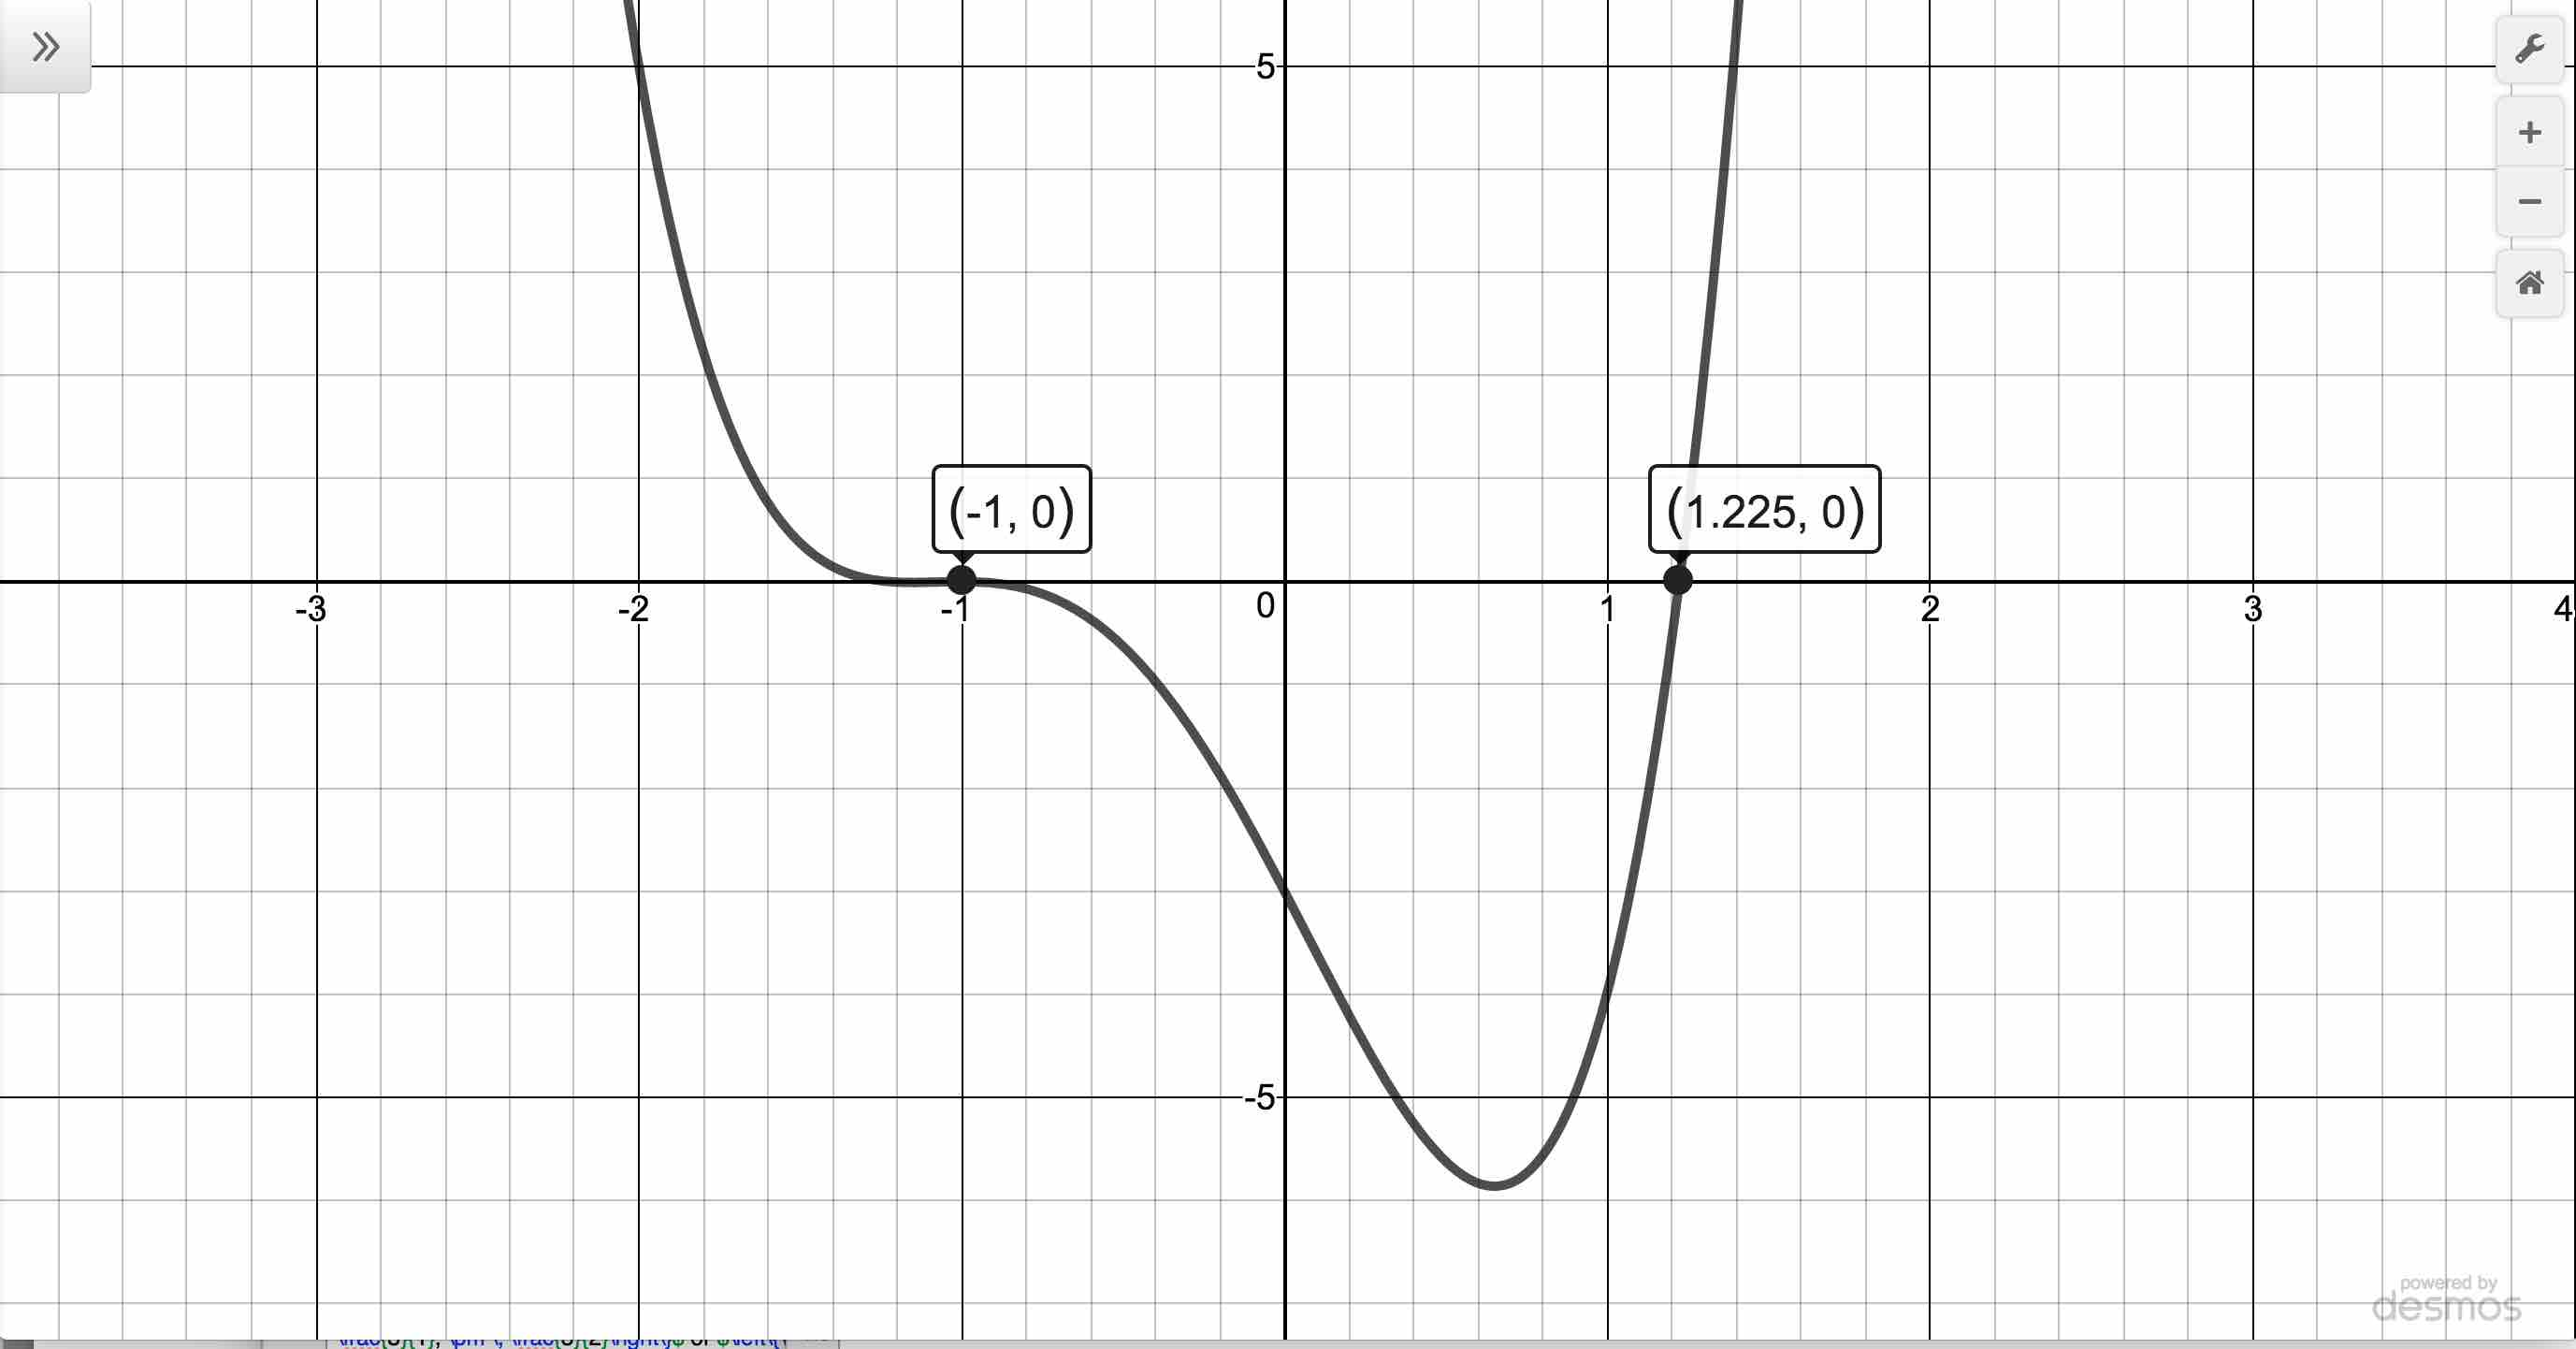
\includegraphics[width = 3in, height=2in]{./RealZerosGraphics/RealZerosEx01a.jpg}  &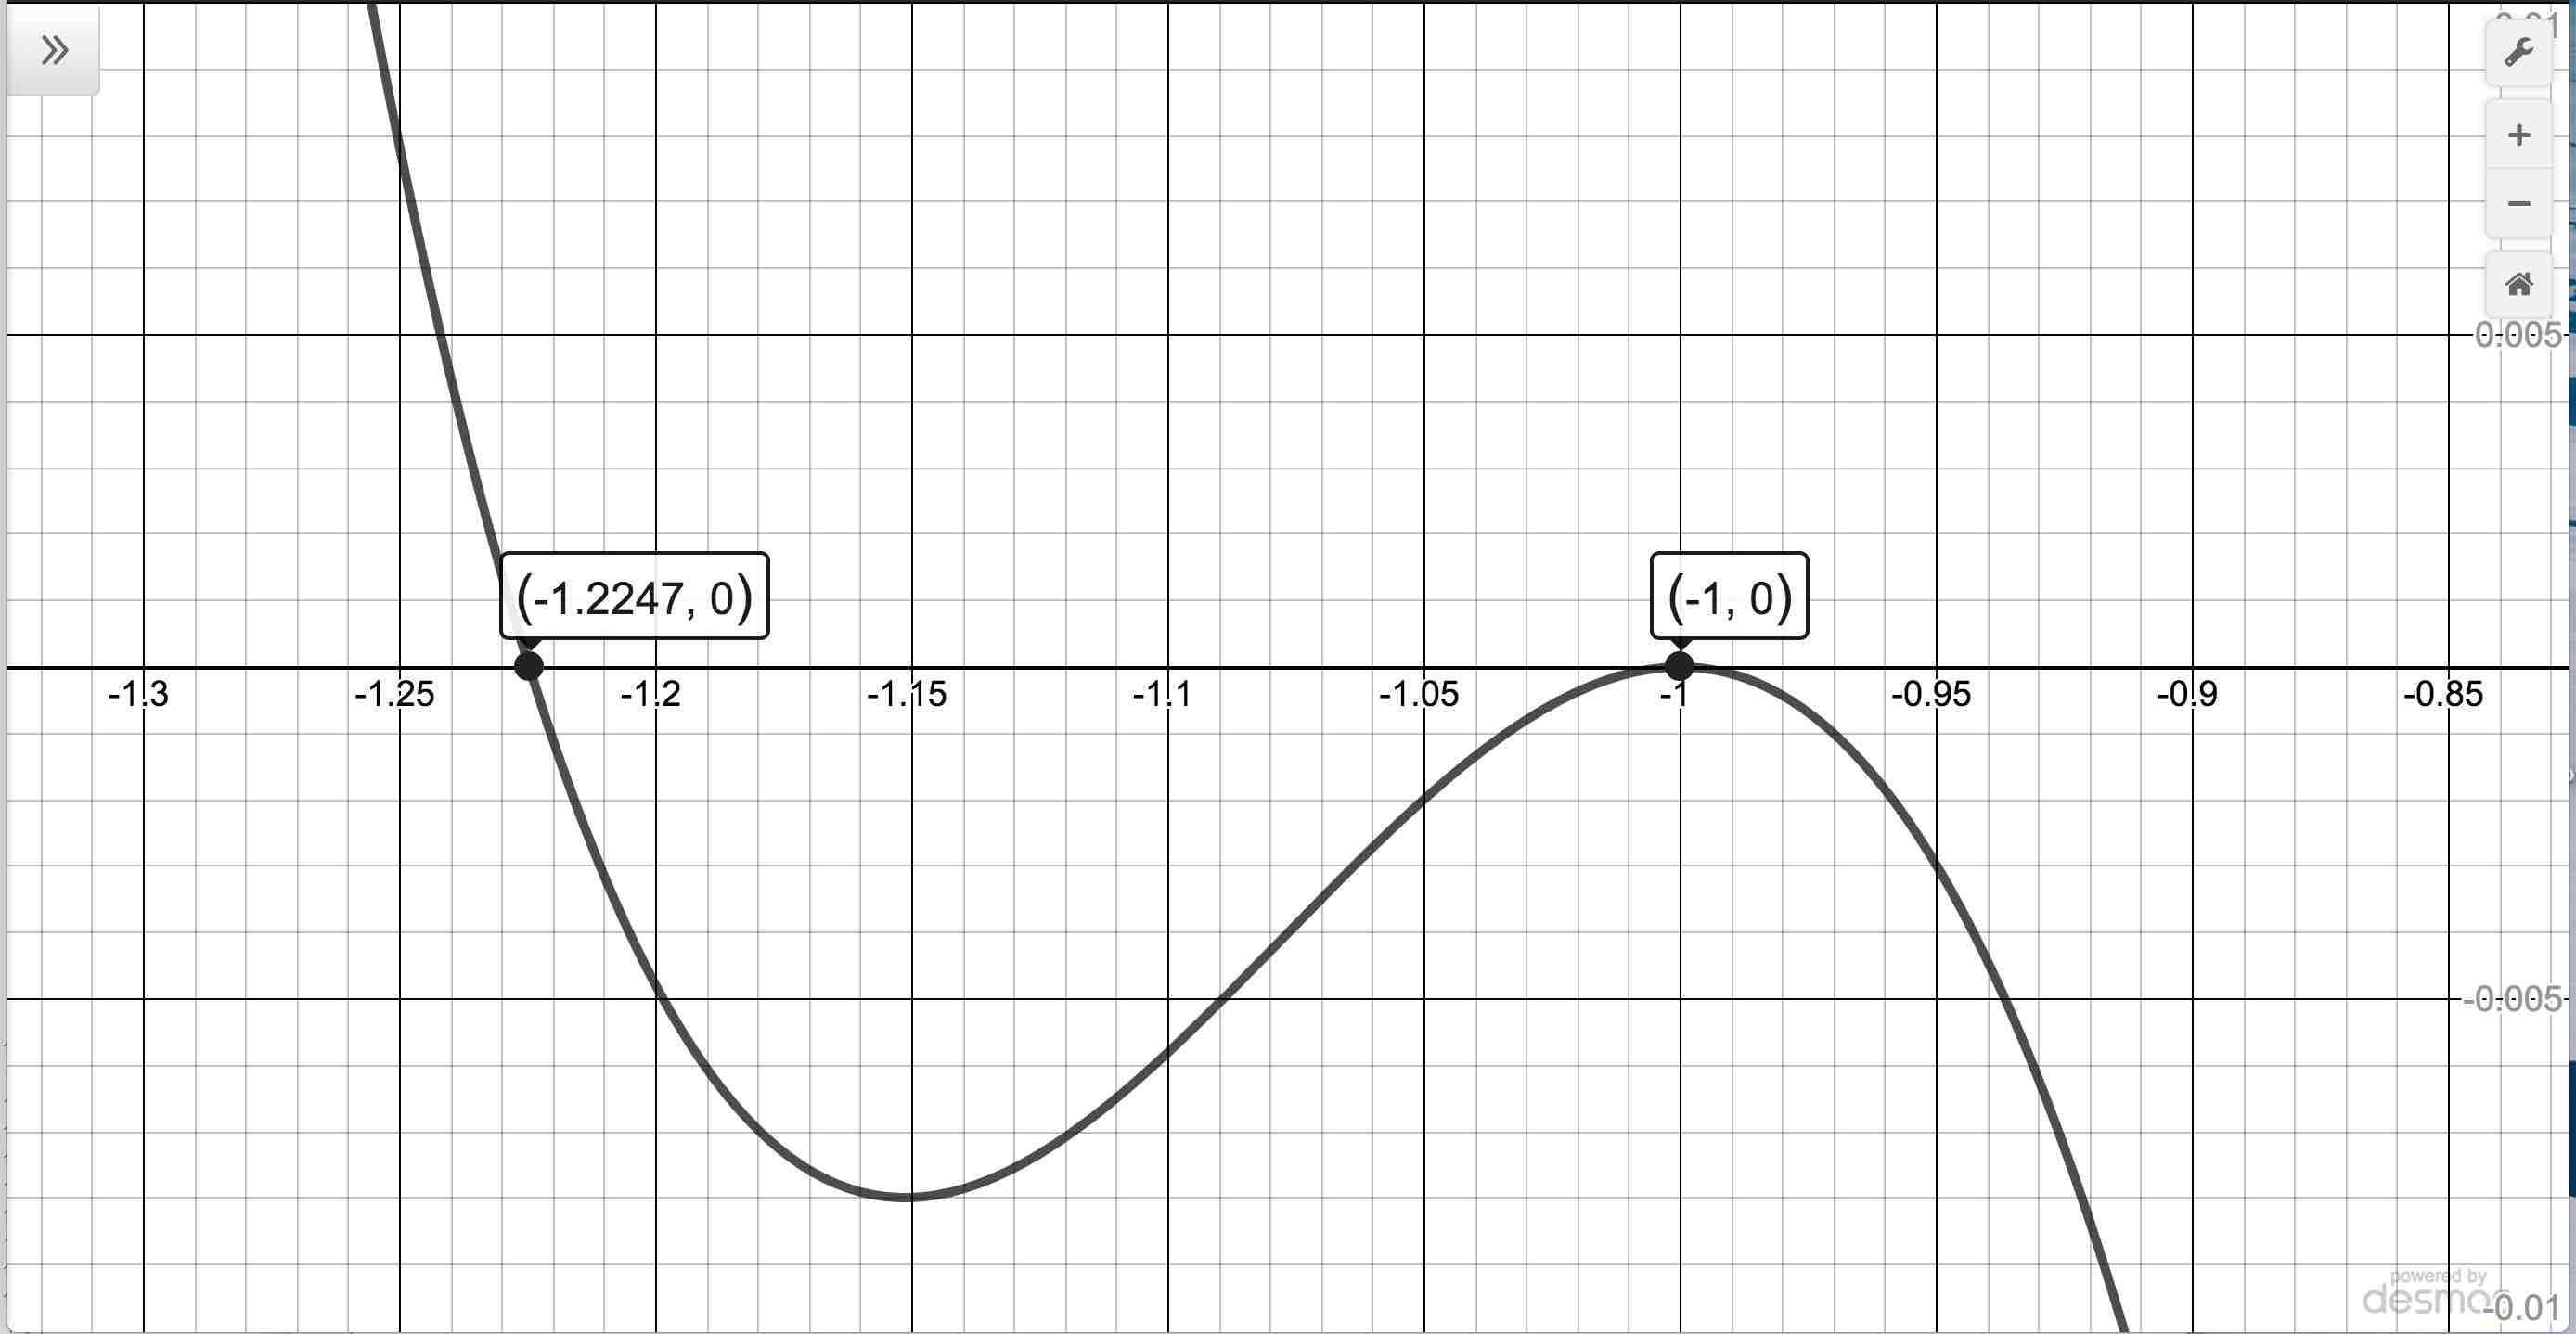
\includegraphics[width = 3in, height=2in]{./RealZerosGraphics/RealZerosEx01b.jpg}

\end{tabular}
\end{center}

 \qed

\end{ex}


Our next example shows how even a mild-mannered polynomial can cause problems.

\begin{ex}  \label{polyquadinform} Let $f(x) = x^4 + x^2 - 12$.

\begin{enumerate}

\item  Use Cauchy's Bound to determine an interval in which all of the real zeros of $f$ lie.

\item  Use the Rational Zeros Theorem to determine a list of possible rational zeros of $f$.

\item  Graph $y=f(x)$ using a graphing utility.

\item  Find all of the real zeros of $f$ and their multiplicities.


\end{enumerate}

{\bf Solution.}

\begin{enumerate}

\item  Applying Cauchy's Bound, we find $M = 12$, so all of the real zeros lie in the interval $[-13,13]$.

\item  Applying the Rational Zeros Theorem with constant term $a_{\mbox{\tiny$0$}} = -12$ and leading coefficient $a_{\mbox{\tiny$4$}} = 1$, we get the list $\{\pm \, 1$, $\pm \, 2$, $\pm \, 3$, $\pm \, 4$, $\pm \, 6$, $\pm \, 12\}$.

\item  Graphing $y=f(x)$ on the interval $[-13,13]$ produces the graph below on the left.  Zooming in a bit gives the graph below on the right.  Based on the graph, none of our rational zeros will work. (Do you see why not?)


\begin{center}

\begin{tabular}{cc}

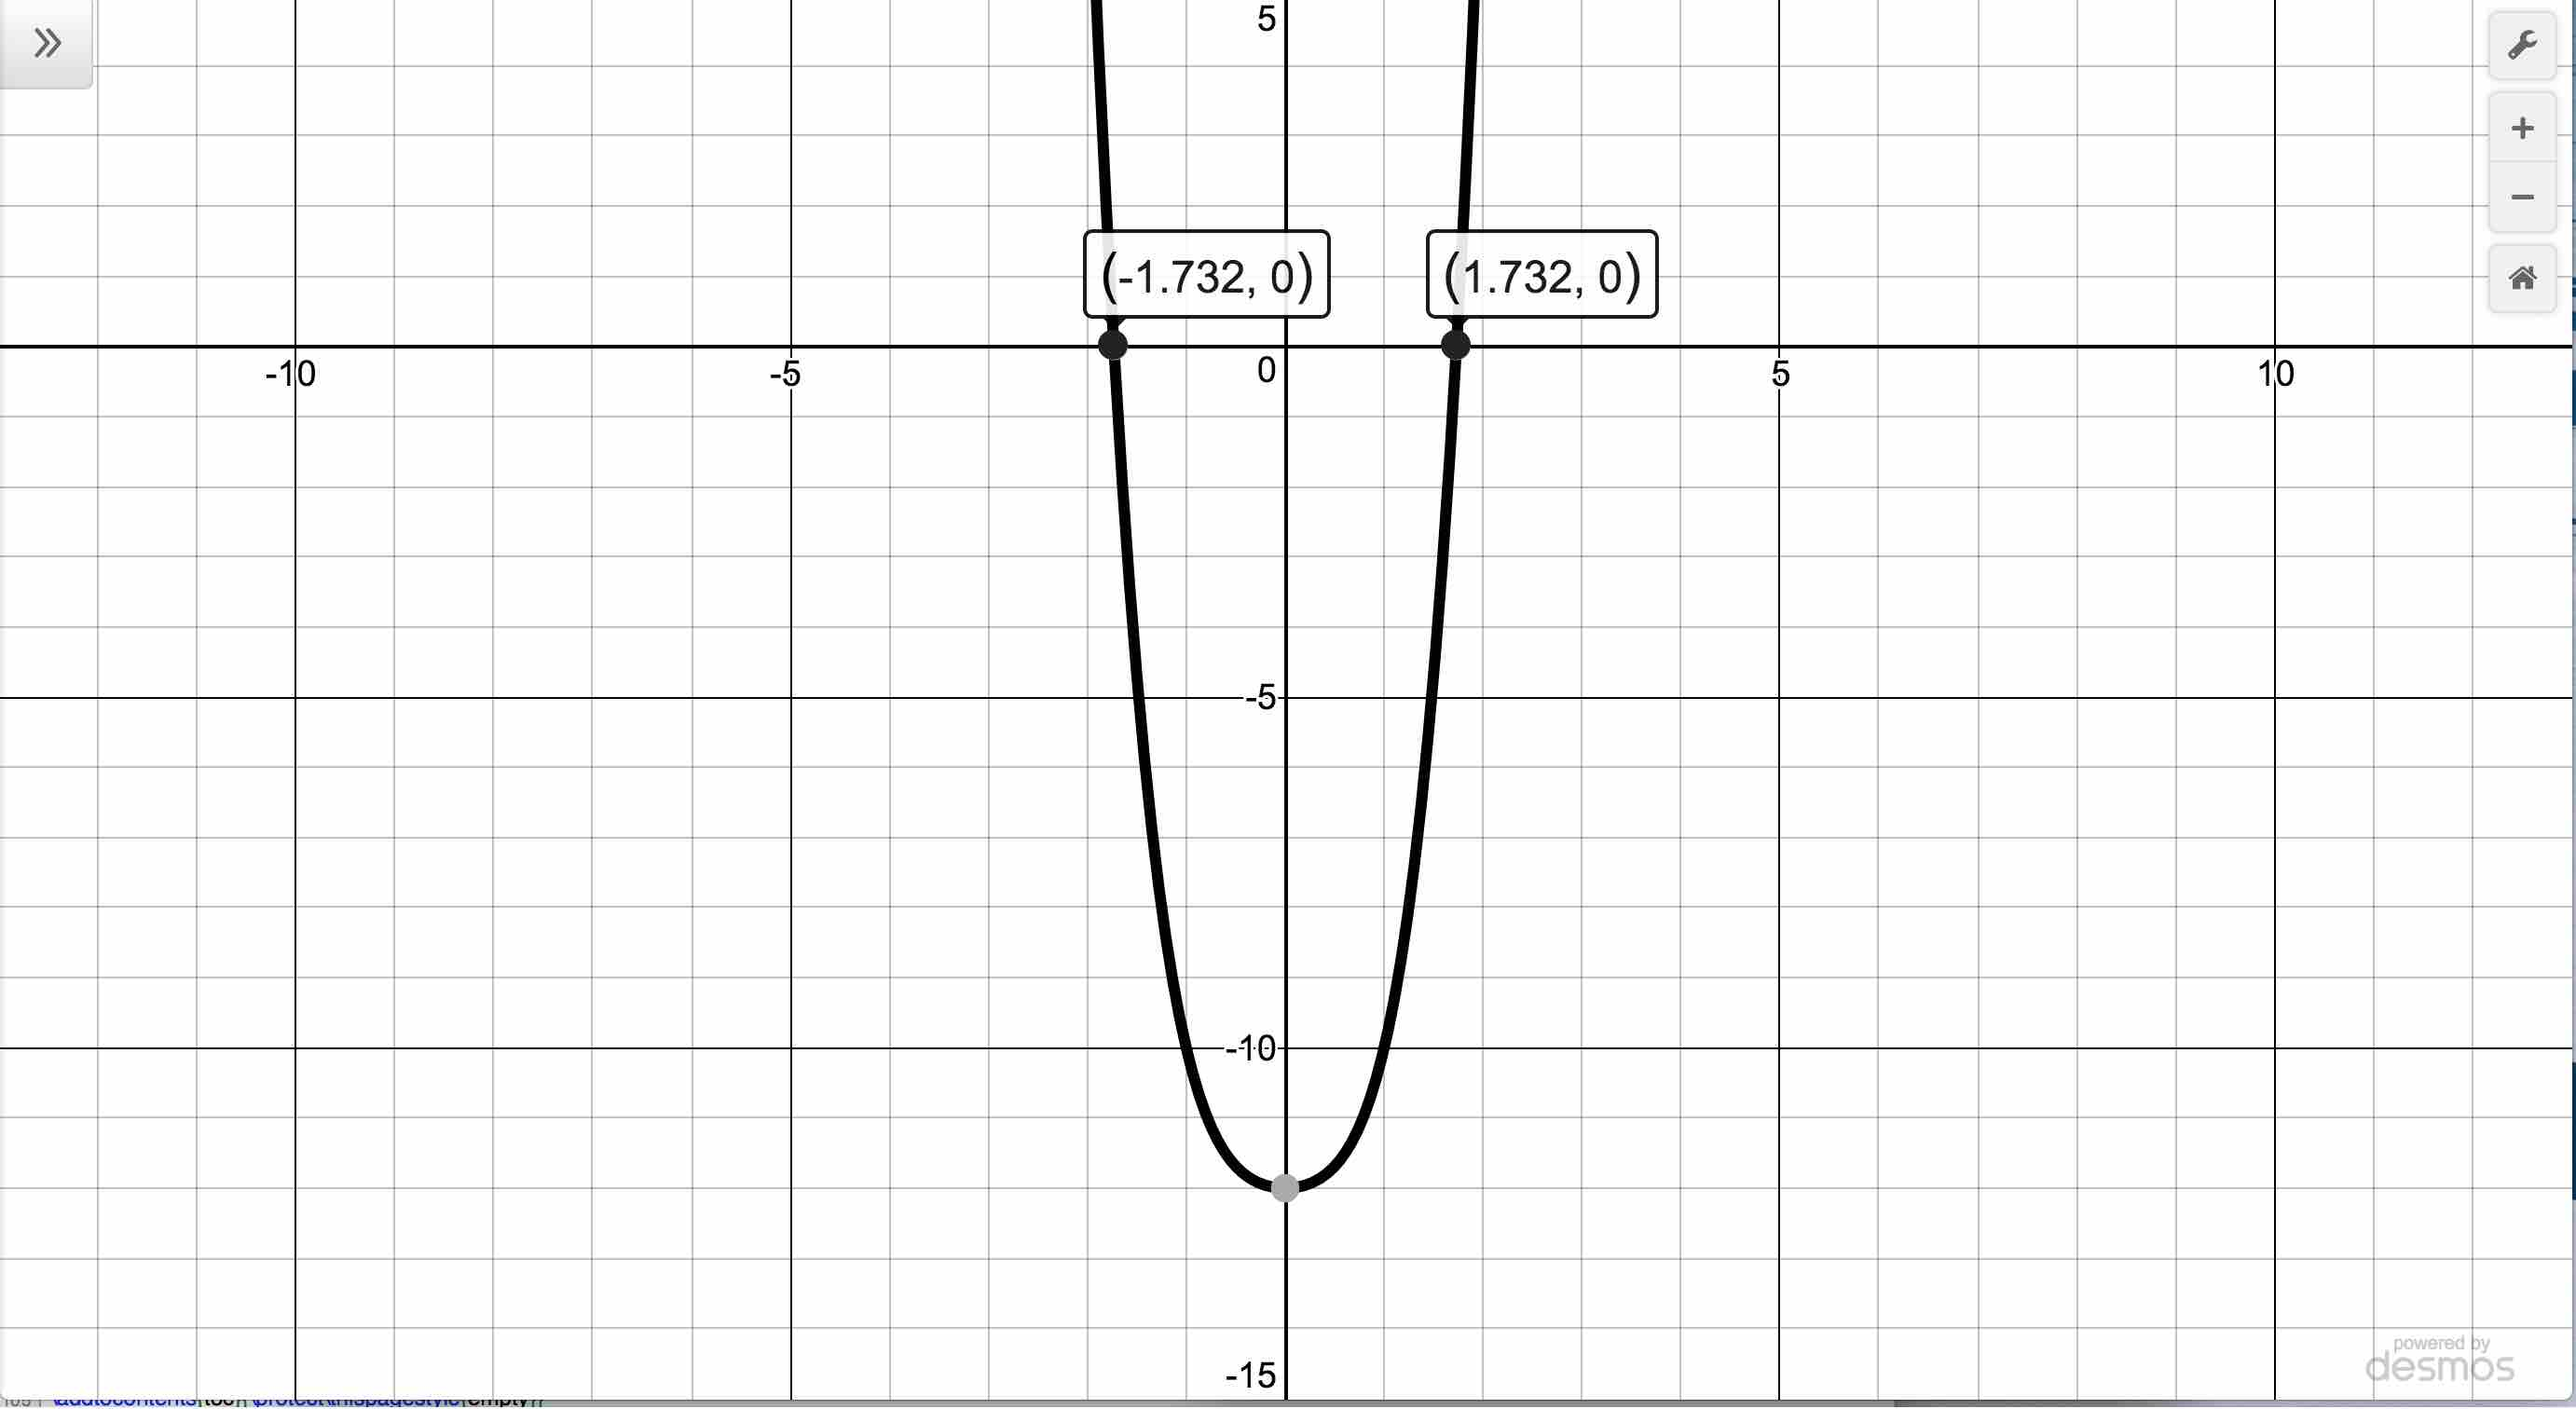
\includegraphics[width = 3in, height=2in]{./RealZerosGraphics/RealZerosEx02a.jpg}  &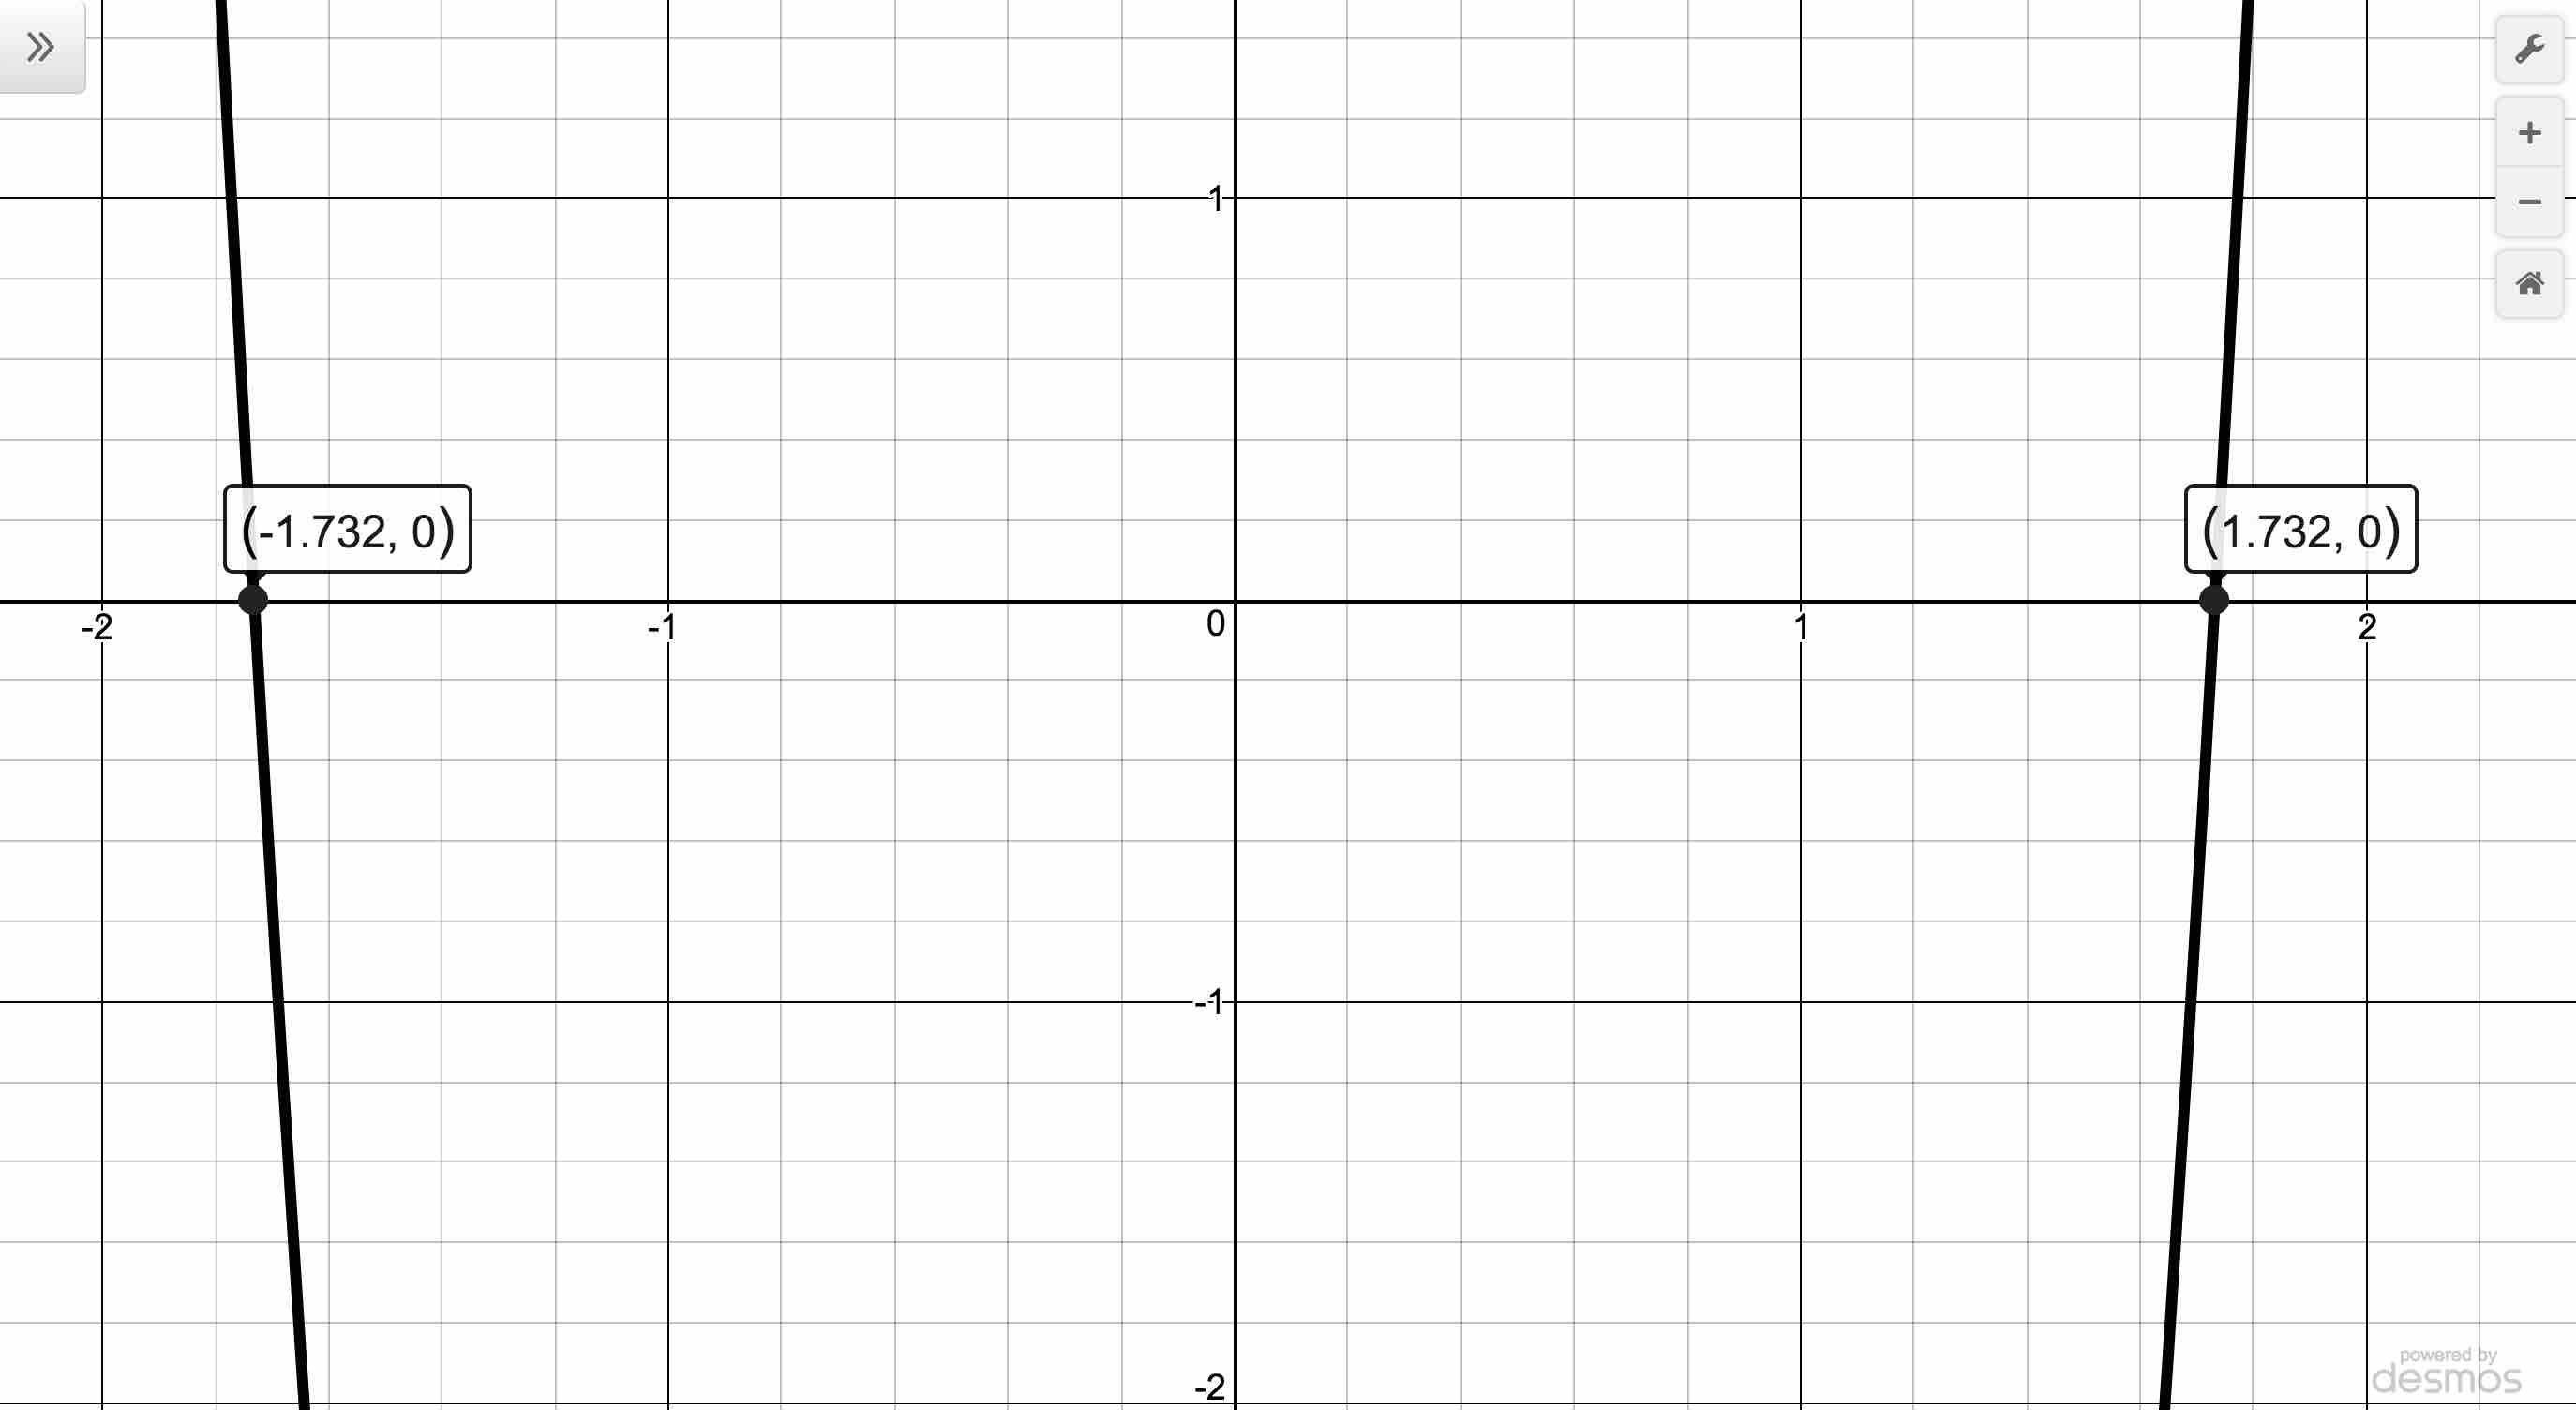
\includegraphics[width = 3in, height=2in]{./RealZerosGraphics/RealZerosEx02b.jpg}

\end{tabular}
\end{center} 

\item  From the graph, we know $f$ has two real zeros, one positive, and one negative.  Our only hope at this point is to try and find the zeros of $f$ by setting $f(x)=x^4+x^2-12=0$ and solving.  If we stare at this equation long enough, we may recognize it as a `quadratic in disguise' or `quadratic in form'. (See Section \ref{AppQuadEqus}.)   In other words, we have three terms: $x^4$, $x^2$ and $12$, and the exponent on the first term, $x^4$, is exactly twice that of the second term, $x^2$.  We may rewrite this as $\left(x^2\right)^2 + \left(x^2\right) - 12 = 0$.  To better see the forest for the trees, we momentarily replace $x^2$ with the variable $u$.  In terms of $u$, our equation becomes $u^2 + u - 12 = 0$, which we can readily factor as $(u+4)(u-3) = 0$.  In terms of $x$, this means $x^4+x^2-12= \left(x^2-3\right) \left(x^2 + 4 \right)=0$. We get $x^2 = 3$, which gives us $x = \pm \sqrt{3}$, or $x^2=-4$, which admits no real solutions.  Since $\sqrt{3} \approx 1.73$, the two zeros match what we expected from the graph.  Turning our attention now to multiplicities, the Factor Theorem guarantees that since $x = \pm \sqrt{3}$ are zeros, $(x- \sqrt{3})$ and $(x + \sqrt{3})$ are factors of $f(x)$.  We've already partially factored  $f(x)$ as $f(x)  = \left(x^2-3\right) \left(x^2 + 4 \right)$.  Since $x^2+4$ as no real zeros, we know both $(x-\sqrt{3})$ and $(x+\sqrt{3})$ must divide $x^2-3$.  By Theorem \ref{nzerosreal},  $x^2-3$ can only have a total of two zeros, including multiplicities, so we are forced to conclude $x = \pm \sqrt{3}$ are each zeros of multiplicity $1$ of $x^2-3$, and hence, $f(x)$.\footnote{Alternatively, we could recognize $x^2 -3 = x^2-(\sqrt{3})^2 = (x-\sqrt{3})(x+\sqrt{3})$, but the above argument works for all quadratic functions, even those which aren't as easy to factor.} \qed

\end{enumerate}

\label{usubex}

\end{ex}

A couple of remarks are in order.  First, the graph of $f(x) = x^4 + x^2 - 12$ appears to be symmetric about the $y$-axis.  Sure enough, we find $f(-x) = (-x)^4+(-x)^2  - 12 = x^4+x^2=12 = f(x)$ proving $f$ is, indeed, an even function, thus \textit{proving} the symmetry \textit{suggested} by the graph.  Second, the technique used to factor $f(x)$ in Example \ref{usubex} is called \index{$u$-substitution} \textbf{{\boldmath $u$}-substitution}.  We shall this technique now and then in the sections to come, so it is worth taking the time to let this idea sink in.  In general, substitution can help us identify a `quadratic in disguise' - in essence, it helps us `see the forest for the trees.'  Last, but not least, it is entirely possible that a polynomial has no real roots at all, or worse, it has real roots but none of the techniques discussed in this section can help us find them exactly.  In the latter case, we are forced to approximate using technology.  


\subsection{For Those Wishing NOT to use a Graphing Calculator}

Suppose we wish to find the zeros of $f(x) = 2x^4+4x^3-x^2-6x-3$ \textit{without} using the calculator.  In this subsection, we present some more advanced mathematical tools (theorems) to help us.  Our first result is due to \href{http://en.wikipedia.org/wiki/Descartes}{\underline{Ren\'{e} Descartes}}.

\smallskip

\colorbox{ResultColor}{\bbm

\begin{thm} \index{Descartes' Rule of Signs}\label{DRS}  \textbf{Descartes' Rule of Signs:}  Suppose $f(x)$ is the formula for a polynomial function written with descending powers of $x$.

\begin{itemize}

\item If $P$ denotes the number of variations of sign in the formula for $f(x)$, then the number of positive real zeros (counting multiplicity) is one of the numbers \{$P$, $P-2$, $P-4$, \ldots \}.

\item If $N$ denotes the number of variations of sign in the formula for $f(-x)$, then the number of negative real zeros (counting multiplicity) is one of the numbers \{$N$, $N-2$, $N-4$, \dots\}.

\end{itemize}

\end{thm}
\ebm}

\smallskip

A few remarks are in order. First, to use Descartes' Rule of Signs, we need to understand what is meant by a \index{polynomial function ! variations in sign}\index{variations in sign}`\textbf{variation in sign}' of a polynomial function.  Consider $f(x) = 2x^4+4x^3-x^2-6x-3$.  If we focus on only the \textit{signs} of the coefficients, we start with a $(+)$, followed by another $(+)$, then switch to $(-)$, and stay $(-)$ for the remaining two coefficients.  Since the signs of the coefficients switched \textit{once} as we read from left to right, we say that $f(x)$ has \textit{one} variation in sign.  When we speak of the variations in sign of a polynomial function $f$ we assume the formula for $f(x)$ is written with descending powers of $x$, as in Definition \ref{polynomialfunction}, and concern ourselves only with the nonzero coefficients.  Second, unlike the Rational Zeros Theorem, Descartes' Rule of Signs gives us an estimate to the \textit{number} of positive and negative real zeros, not the actual \textit{value} of the zeros. Lastly, Descartes' Rule of Signs counts multiplicities.  This means that, for example, if one of the zeros has multiplicity $2$, Descsartes' Rule of Signs would count this as \textit{two} zeros.  Lastly, note that the number of positive or negative real zeros always starts with the number of sign changes and decreases by an even number.  For example, if $f(x)$ has $7$ sign changes, then, counting multplicities, $f$ has either $7$, $5$, $3$ or $1$ positive real zero.  This implies that the graph of $y=f(x)$ crosses the positive $x$-axis at least once.  If $f(-x)$ results in $4$ sign changes, then, counting multiplicities, $f$ has $4$, $2$ or $0$ negative real zeros;  hence, the graph of $y=f(x)$ may not cross the negative $x$-axis at all.  The proof of Descartes' Rule of Signs is a bit technical, and can be found \href{http://www.cut-the-knot.org/fta/ROS2.shtml}{\underline{here}}. 

\begin{ex}  Let $f(x) = 2x^4+4x^3-x^2-6x-3$.  Use Descartes' Rule of Signs to determine the possible number and location of the real zeros of $f$.

\smallskip

{\bf Solution.}  As noted above, the variations of sign of $f(x)$ is $1$. This means, counting multiplicities, $f$ has exactly $1$ positive real zero.  Since $f(-x)=2(-x)^4+4(-x)^3-(-x)^2-6(-x)-3=2x^4-4x^3-x^2+6x-3$ has $3$ variations in sign, $f$ has either $3$ negative real zeros or $1$ negative real zero, counting multiplicities. \qed

\label{DRSex}

\end{ex}

Cauchy's Bound gives us a general bound on the zeros of a polynomial function.  Our next result helps us determine bounds on the real zeros of a polynomial as we synthetically divide which are often sharper\footnote{That is, better, or more accurate.} bounds than Cauchy's Bound.   

\smallskip

\colorbox{ResultColor}{\bbm
\begin{thm}  \label{ULbounds} \textbf{Upper and Lower Bounds:}  Suppose $f$ is a polynomial of degree $n \geq 1$. \index{Upper and Lower Bounds Theorem}\index{polynomial function ! zero ! upper bound}\index{polynomial function ! zero ! lower bound}\index{zero ! upper and lower bounds}

\begin{itemize}

\item  If $c > 0$ is synthetically divided into $f$ and all of the numbers in the final line of the division tableau have the same signs, then $c$ is an upper bound for the real zeros of $f$.  That is, there are no real zeros greater than $c$.

\item  If $c < 0$ is synthetically divided into $f$ and the numbers in the final line of the division tableau alternate signs, then $c$ is a lower bound for the real zeros of $f$.  That is, there are no real zeros less than $c$.

\textbf{NOTE:}  If the number $0$ occurs in the final line of the division tableau in either of the above cases, it can be treated as $(+)$ or $(-)$ as needed.

\end{itemize}

\end{thm}
\ebm}


\smallskip

The Upper and Lower Bounds Theorem works because of Theorem \ref{polydivthm}.  For the upper bound part of the theorem, suppose $c>0$ is divided into $f$ and the resulting line in the division tableau contains, for example, all nonnegative numbers.  This means $f(x) = (x-c) q(x) + r$, where the coefficients of the quotient polynomial and the remainder are nonnegative.  (Note that the leading coefficient of $q$ is the same as $f$ so $q(x)$ is not the zero polynomial.)  If $b > c$, then $f(b) = (b-c) q(b) + r$, where $(b-c)$ and  $q(b)$ are both positive and $r \geq 0$.  Hence $f(b) > 0$ which shows $b$ cannot be a zero of $f$.  Thus no real number $b > c$ can be a zero of $f$, as required.  A similar argument proves $f(b) < 0$ if all of the numbers in the final line of the synthetic division tableau are non-positive.  To prove the lower bound part of the theorem, we note that a lower bound for the negative real zeros of $f(x)$ is an upper bound for the positive real zeros of $f(-x)$, since all we are doing is reflecting the numbers across the $x=0$.  Applying the upper bound portion to $f(-x)$ gives the result.  (Do you see where the alternating signs come in?) With the additional mathematical machinery of Descartes' Rule of Signs and the Upper and Lower Bounds Theorem, we can find the real zeros of $f(x) = 2x^4+4x^3-x^2-6x-3$ without the use of a graphing utility.

\begin{ex}  Let $f(x) = 2x^4+4x^3-x^2-6x-3$.

\begin{enumerate}

\item  Find all of the real zeros of $f$ and their multiplicities.

\item Sketch the graph of $y=f(x)$.

\end{enumerate}  

{\bf Solution.}  \begin{enumerate}

\item  We know from Cauchy's Bound that all of the real zeros lie in the interval $[-4,4]$ and that our possible rational zeros are $\pm \, \frac{1}{2}$, $\pm \, 1$, $\pm \, \frac{3}{2}$ and $\pm \, 3$.  Descartes' Rule of Signs guarantees us at least one negative real zero and exactly one positive real zero, counting multiplicity.  We try our positive rational zeros, starting with the smallest, $\frac{1}{2}$.  Since the remainder isn't zero, we know $\frac{1}{2}$ isn't a zero.  Sadly, the final line in the division tableau has both positive and negative numbers, so $\frac{1}{2}$ is not an upper bound.  The only information we get from this division is courtesy of the Remainder Theorem which tells us $f\left(\frac{1}{2}\right) =  -\frac{45}{8}$ so the point $\left(\frac{1}{2}, -\frac{45}{8}\right)$ is on the graph of $f$.  We continue to our next possible zero, $1$.  As before, the only information we can glean from this is that $(1,-4)$ is on the graph of $f$.  When we try our next possible zero, $\frac{3}{2}$, we get that it is not a zero, and we also see that it is an upper bound on the zeros of $f$, since all of the numbers in the final line of the division tableau are positive.  This means there is no point trying our last possible rational zero, $3$.  Descartes' Rule of Signs guaranteed us a positive real zero, and at this point we have shown this zero is irrational.\footnote{Since polynomials are continuous, we know the zero lies between $1$ and $\frac{3}{2}$, since $f(1) < 0$ and $f\left(\frac{3}{2}\right) > 0$.}

 
\begin{tabular}{ccc}

$\begin{array}{rrrrrr}

 \frac{1}{2} \, \, \vline& 2 & 4 & -1  & -6 & -3 \\

  & \downarrow     &  1  &  \frac{5}{2}  & \frac{3}{4} & -\frac{21}{8} \\ [4pt] \hhline{~-----}
  
  &  2            &   5  &  \frac{3}{2} & -\frac{21}{4} &  \fbox{$-\frac{45}{8}$}  \\

\end{array}$ &     

$\begin{array}{rrrrrr}

1 \, \, \vline& 2 & 4 & -1  & -6 & -3 \\

  & \downarrow     &  2 &  6  & 5 & -1 \\ [4pt] \hhline{~-----}
  
  &  2            &   6  &  5 & -1 &  \fbox{$-4$}  \\

\end{array}$  &

             
$\begin{array}{rrrrrr}

\frac{3}{2} \, \, \vline& 2 & 4 & -1  & -6 & -3 \\

  & \downarrow     &  3 &  \frac{21}{2}  & \frac{57}{4} & \frac{99}{8} \\ [4pt] \hhline{~-----}
  
  &  2            &   7  &  \frac{19}{2} & \frac{33}{4} &  \fbox{$\frac{75}{8}$}  \\

\end{array}$

\end{tabular}

\smallskip

We now turn our attention to negative real zeros.  We try the largest possible zero, $-\frac{1}{2}$.  Synthetic division shows us it is not a zero, nor is it a lower bound (since the numbers in the final line of the division tableau do not alternate), so we proceed to $-1$.  This division shows $-1$ is a zero.  Descartes' Rule of Signs told us that we may have up to three negative real zeros, counting multiplicity, so we try $-1$ again, and it works once more.  At this point, we have taken $f$, a fourth degree polynomial, and performed two successful divisions.  Our quotient polynomial is quadratic, so we look at it to find the remaining zeros.

\begin{tabular}{cc}

$\begin{array}{rrrrrr}

 -\frac{1}{2} \, \, \vline& 2 & 4 & -1  & -6 & -3 \\

  & \downarrow     &  -1  &  -\frac{3}{2}  & \frac{5}{4} & \frac{19}{8} \\ [4pt] \hhline{~-----}
  
  &  2            &   3  &  -\frac{5}{2} & -\frac{19}{4} &  \fbox{$-\frac{5}{8}$}  \\

\end{array}$ &  \hspace{1in}

$\begin{array}{rrrrrr}
 -1 \, \, \vline& 2 & 4 & -1  & -6 & -3 \\

  & \downarrow     &  -2  &  -2  & 3 & 3\\ \hhline{~-----} 
  
  -1 \, \, \vline&  2 &   2  & -3 & -3 &  \fbox{$0$}  \\
    
               & \downarrow &  -2  &  0  & 3 &\\ \hhline{~----} 
 
   & 2  &   0  & -3& \fbox{0} &   \\
  
        

\end{array}$  

\end{tabular}

\smallskip

Setting the quotient polynomial equal to zero yields $2x^2 - 3 = 0$, so that $x^2 = \frac{3}{2}$, or $x = \pm \, \frac{\sqrt{6}}{2}$.  Descartes' Rule of Signs tells us that the positive real zero we found, $\frac{\sqrt{6}}{2}$, has multiplicity $1$.  Descartes also tells us the total multiplicity of negative real zeros is $3$, which forces $-1$ to be a zero of multiplicity $2$ and $- \frac{\sqrt{6}}{2}$ to have multiplicity $1$.  

\item  We know the end behavior of $y=f(x)$ resembles that of its leading term $y=2x^4$.  This means that the graph enters the scene in Quadrant II and exits in Quadrant I.  Since $\pm \, \frac{\sqrt{6}}{2}$ are zeros of multiplicity $1$, we have that the graph crosses through the $x$-axis at the points $\left( -\frac{\sqrt{6}}{2}, 0 \right)$ and $\left( \frac{\sqrt{6}}{2}, 0 \right)$ in a fairly linear fashion.  Since $-1$ is a zero of multiplicity $2$, the graph of $y=f(x)$ touches and rebounds off the $x$-axis at $(-1,0)$ in a parabolic manner.  Last, but not least, since $f(0) = -3$, we get the  $y$-intercept is $(0,-3)$.  Putting all of this together results in the graph below.

\begin{center}

\begin{mfpic}[20]{-4}{4}{-5}{4}
\axes
\tlabel[cc](4,-0.5){\scriptsize $x$}
\tlabel[cc](0.5,4){\scriptsize $y$}
\scriptsize
\tlabel[cc](-4,-0.5){\scriptsize $\left( -\frac{\sqrt{6}}{2}, 0 \right)$}
\tlabel[cc](2,-0.5){\scriptsize $\left( \frac{\sqrt{6}}{2}, 0 \right)$}
\tlabel[cc](-0.75,-1){\scriptsize $(0, -3)$}
\tlabel[cc](-1,0.5){\scriptsize $(-1, 0)$}
\normalsize
\penwd{1.25pt}
\arrow \reverse \arrow \function{-3.5,3.25,0.1}{0.1*(x+3)*((x+1)**2)*(x-3)}
\point[4pt]{(-3,0),(-1,0),(3,0), (0,-0.9)}
\tcaption{\scriptsize $y = f(x) = 2x^4+4x^3-x^2-6x-3$}
\end{mfpic}

\end{center}

\qed

\end{enumerate}

\end{ex}

\subsection{The Intermediate Value Theorem and Inequalities}
\label{IVTaninequalities}

As we mentioned in Section \ref{GraphsofPolynomials}, polynomial functions are continuous.  An important property of continuous functions is that they cannot change sign between  two values unless there is a zero in between.  We used this property of quadratic functions when constructing sign diagrams to help us solve inequalities (see Section \ref{QuadraticInequalities}.)   This property is a version of the celebrated  \textbf{Intermediate Value Theorem}. 


\colorbox{ResultColor}{\bbm

\begin{thm} \textbf{The Intermediate Value Theorem (Zero Version):} If $f$ is continuous over an interval containing $a$ and $b$ and $f(a)$ and $f(b)$ have different signs, then $f$ has a zero between $a$ and $b$.  That is, for at least one value $c$ between $a$ and $b$, $f(c) = 0$. \index{Intermediate Value Theorem ! polynomial zero version}

\label{IVT}
\end{thm}

\ebm}

The Intermediate Value Theorem is discussed in greater detail in Calculus, and its proof is usually delayed until a formal analysis course.  It is an example of an `existence' theorem - it tells us that, under suitable conditions, a zero exists - but offers us no algorithm to find it.\footnote{See the notes on the `Bisection Method' at the end of this section.} Its use to us in this section is that it provides the justification needed to create sign diagrams for general polynomial functions in the same manner in which we constructed them for quadratic functions.

\colorbox{ResultColor}{\bbm

\centerline{\textbf{Steps for Constructing a Sign Diagram for a Polynomial Function}}


Suppose $f$ is a polynomial function. \index{sign diagram ! polynomial function}

\begin{enumerate}

\item  Find the zeros of $f$ and place them on the number line with the number $0$ above them.

\item  Choose a real number, called a \textbf{test value}, in each of the intervals determined in step 1. 

\item  Determine and record the sign of $f(x)$ for each test value in step 2.

\end{enumerate}

\ebm}

The Intermediate Value Theorem justifies the use of just one `test' value in the algorithm above, since a continuous function cannot change signs on an interval without there being a zero on that interval.  Since we have found the zeros in Step 1 of the algorithm and used these to create the intervals for Step 2, there cannot be any sign changes on any of the intervals in Step 2.

Not surprisingly, we use sign diagrams to solve inequalities involving higher order polynomial functions in the same way we used them to solve inequalities involving quadratic functions. We reproduce our algorithm from section \ref{QuadraticInequalities} for reference.


\colorbox{ResultColor}{\bbm

\centerline{\textbf{Solving Inequalities using Sign Diagrams}} \index{inequality ! solution using sign diagram }

To solve an inequality using a sign diagram:

\begin{enumerate}

\item  Rewrite the inequality so a function $f(x)$ is being compared to `$0$.'

\item  Make a sign diagram for $f$.

\item  Record the solution.

\end{enumerate}

\ebm}


\begin{ex}  \label{polyeqineqexample} $~$

\begin{enumerate}

\item  Find all of the real solutions to the equation $2x^5+6x^3+3 = 3x^4+8x^2$. 

\item  Solve the inequality $2x^5+6x^3+3 \leq 3x^4+8x^2$.

\item  Interpret your answer to part 2 graphically, and verify using a graphing utility.


\end{enumerate}

{\bf Solution.} 

\begin{enumerate}

\item  Finding the real solutions to $2x^5+6x^3+3 = 3x^4+8x^2$ is the same as finding the real solutions to $2x^5-3x^4+6x^3-8x^2+3=0$.  In other words, we are looking for the real zeros of $p(x)=  2x^5-3x^4+6x^3-8x^2+3$.  Using the techniques developed in this section, we get

\[\begin{array}{rrrrrrr}
1 \, \, \vline& 2 & -3 & 6  & -8 & 0 &3 \\

  & \downarrow     &  2  &  -1  & 5 & -3 & -3\\ \hhline{~------} 

 1 \, \, \vline& 2 & -1 & 5  & -3 & -3 & \fbox{$0$} \\

  & \downarrow     &  2 &  1  & 6 & 3 &\\ \hhline{~-----} 
  
  -\frac{1}{2} \, \, \vline&  2 &  1  & 6 & 3 &  \fbox{$0$} & \\
    
               & \downarrow &  -1  &  0  & -3 &&\\ \hhline{~----} 
 
   & 2  &   0  & 6& \fbox{0} &&   \\
  


\end{array}\]


The quotient polynomial is $2x^2 + 6$ which has no real zeros so we get $x=-\frac{1}{2}$ and $x=1$.   

\item Our first step is to rewrite this inequality so as to compare a function $f(x)$ to $0$.  We have two options, but choose $2x^5-3x^4+6x^3-8x^2+3 \leq 0$, since  we found the zeros of $p(x) = 2x^5-3x^4+6x^3-8x^2+3$ to be $x=-\frac{1}{2}$ and $x=1$. We construct our sign diagram below using the test values $-1$, $0$, and $2$.

\begin{center}

\begin{mfpic}[10]{-5}{5}{-2}{2}
\arrow \reverse \arrow \polyline{(-5,0),(5,0)}
\xmarks{-2,2}
\arrow \polyline{(-3.5,-1.5),(-3.5,-0.5)}
\arrow \polyline{(0,-1.5),(0,-0.5)}
\arrow \polyline{(3.5,-1.5),(3.5,-0.5)}
\tlpointsep{4pt}
\axislabels {x}{{$-\frac{1}{2} \hspace{7pt}$} -2, {$1$} 2}
\tlabel[cc](-3.5,1){$(-)$}
\tlabel[cc](-2,1){$0$}
\tlabel[cc](0,1){$(+)$}
\tlabel[cc](2,1){$0$}
\tlabel[cc](3.5,1){$(+)$}
\tlabel[cc](-3.5,-2.25){$-1$}
\tlabel[cc](0,-2.25){$0$}
\tlabel[cc](3.5,-2.25){$2$}
\end{mfpic} 

\end{center}

The solution to $p(x) < 0$ is $\left(-\infty, -\frac{1}{2}\right)$, and we know $p(x) = 0$ at $x=-\frac{1}{2}$ and $x=1$.  Hence, the solution to $p(x) \leq 0$ is $\left(-\infty, -\frac{1}{2}\right] \cup \left\{1\right\}$.  


\item To interpret this solution graphically, we set $f(x) = 2x^5+6x^3+3$ and $g(x) = 3x^4+8x^2$.  Recall from Section \ref{AbsoluteValueFunctions} the solution to $f(x) \leq g(x)$ is the set of $x$ values for which the graph of $f$ is below the graph of $g$ (where $f(x) < g(x)$) along with the $x$ values where the two graphs intersect ($f(x) = g(x)$).  Graphing $f$ and $g$ using a graphing utility produces the graph below on the left.  (The end behavior should tell you which is which.)  We see that the graph of $f$ is below the graph of $g$ on $\left(-\infty, -\frac{1}{2}\right)$. However, it is difficult to see what is happening near $x=1$.  Zooming in (and making the graph of $g$ lighter), we see that the graphs of $f$ and $g$ do intersect at $x=1$, but the graph of $g$ remains below the graph of $f$ on either side of $x = 1$.

\begin{center}

\begin{tabular}{cc}

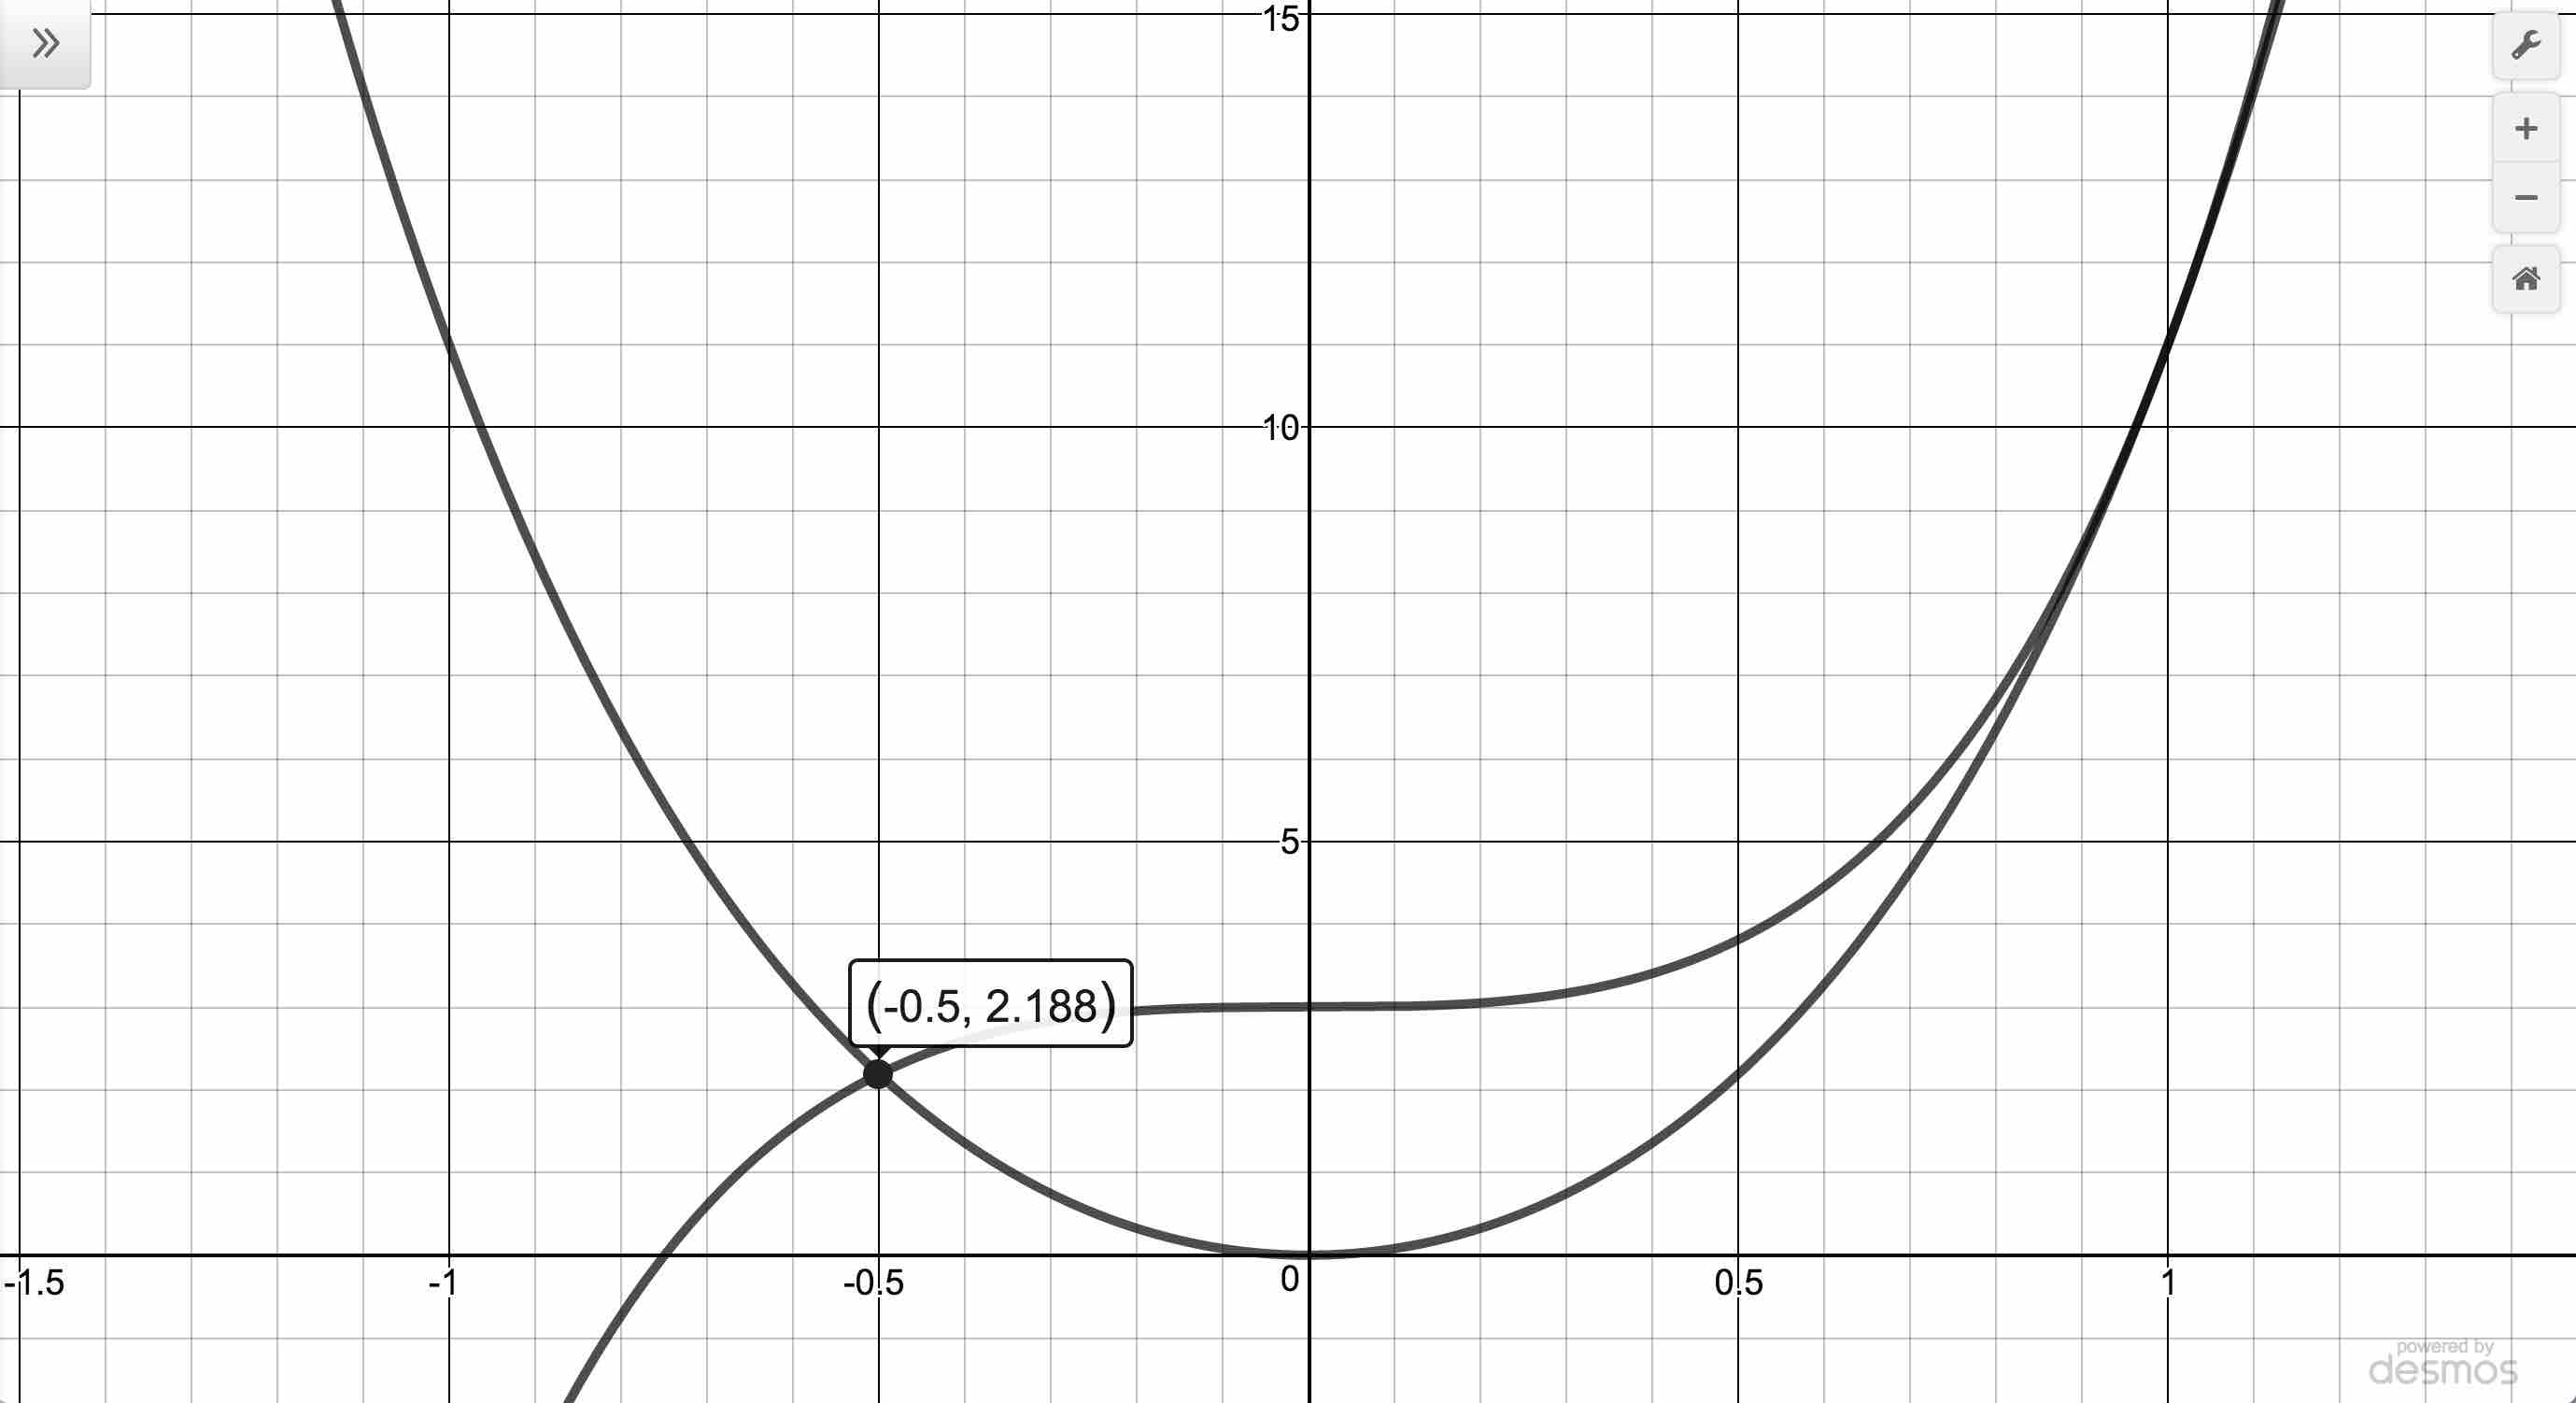
\includegraphics[width = 3in, height=2in]{./RealZerosGraphics/RealZerosEx03a.jpg}  &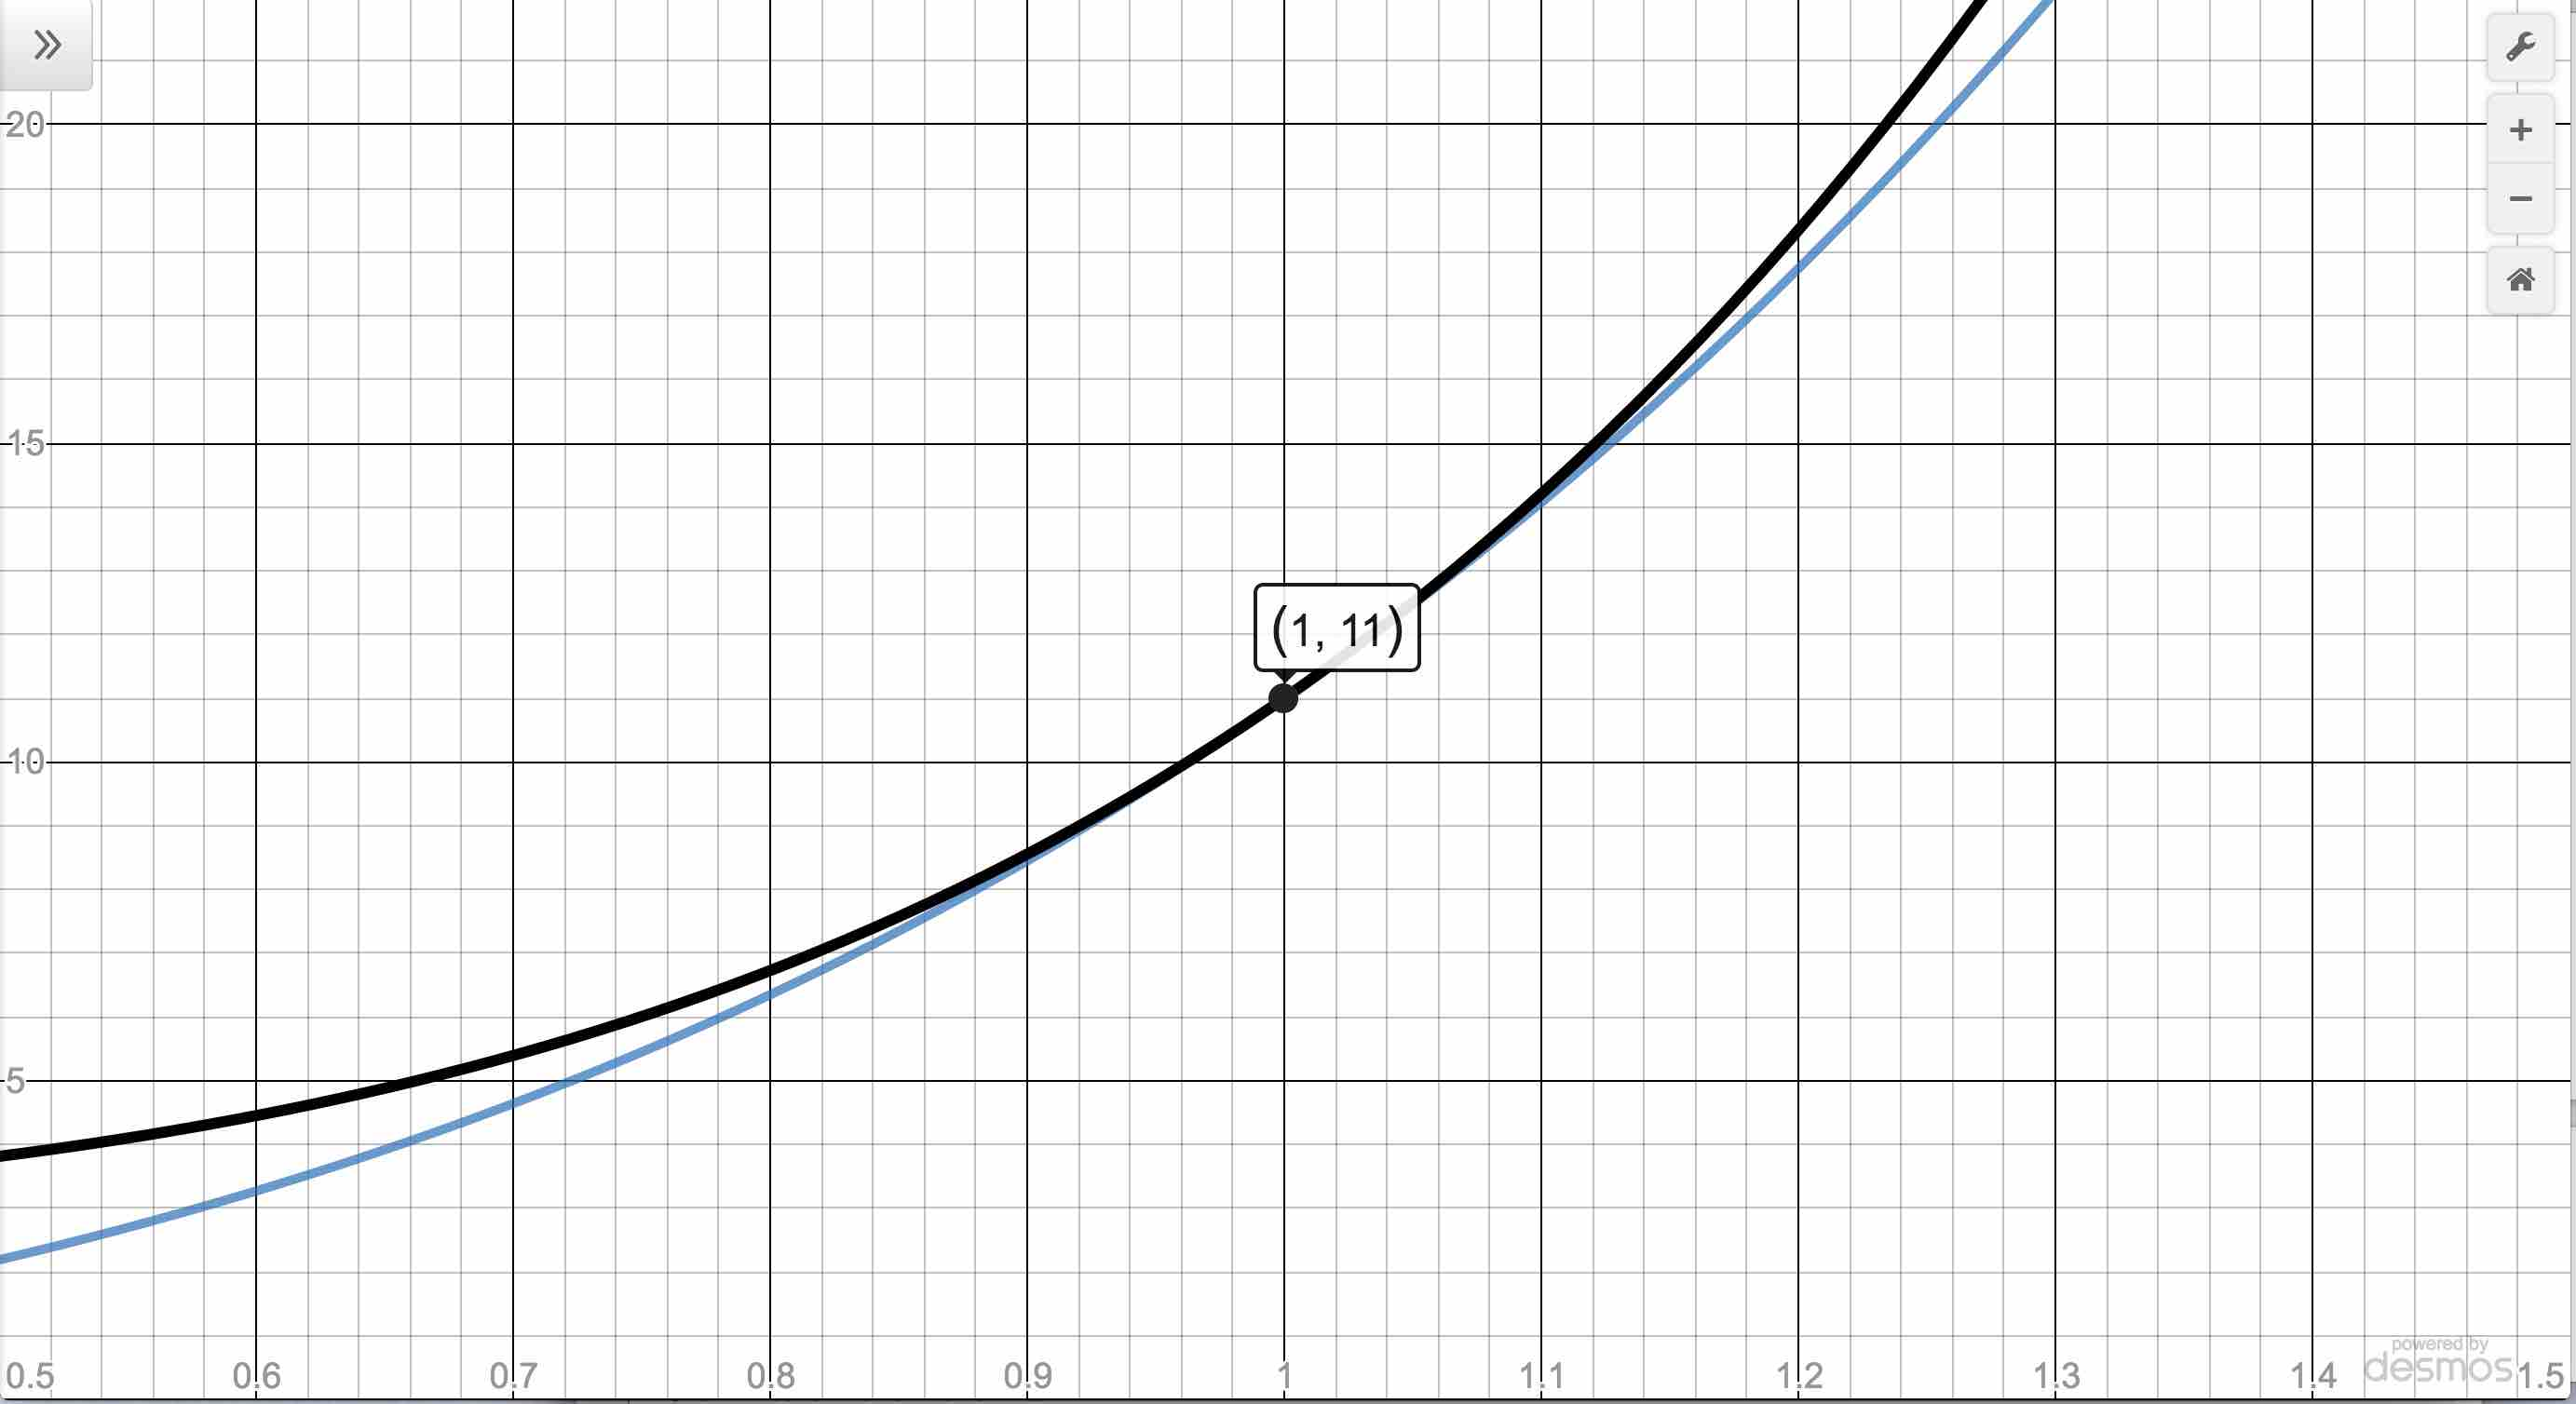
\includegraphics[width = 3in, height=2in]{./RealZerosGraphics/RealZerosEx03b.jpg}

\end{tabular}
\end{center} 

\qed
\end{enumerate}

\end{ex}

Note that we could have used end behavior and the concept of multiplicity to create the sign diagram used in Example \ref{polyeqineqexample} as follows.  We know the end behavior of $p(x) = 2x^5-3x^4+6x^3-8x^2+3$ matches that of $y = 2x^5$ which means as $x \rightarrow -\infty$, $p(x) \rightarrow -\infty$.  This means for the interval $\left(-\infty, -\frac{1}{2}\right)$, $p(x) < 0$ or $(-)$. From our work finding the zeros of $p$, we can deduce the multiplicity of the zero $x = -\frac{1}{2}$ is $1$ which means the graph of $y = p(x)$ crosses through the $x$-axis at $\left( -\frac{1}{2}, 0 \right)$, hence, changing sign from $(-)$ to $(+)$.  Finally, we can deduce the multiplicity of the zero $x = 1$ is $2$ which means the graph of $y = p(x)$ rebounds here, meaning the sign of $p(x)$ for $x > 1$ is $(+)$.  This matches the end behavior, since as $x \rightarrow \infty$, $p(x) \rightarrow \infty$.  The reader is encouraged to tackle any given problem using whatever tools are comfortable and convenient, but it also never hurts to think outside the box and revisit a problem from a variety of perspectives.

Next up is an application problem torn  from page \pageref{LCDmaxprofit} in the Exercises of Section \ref{GraphsofPolynomials}.

\begin{ex} Suppose the profit $P$, in \textit{thousands} of dollars, from producing and selling $x$ \textit{hundred} LCD TVs is given by  $P(x)=-5x^3+35x^2-45x-25$, $0 \leq x \leq 10.07$.  How many TVs should be produced to make a profit?  Check your answer using a graphing utility.

\smallskip

{\bf Solution.}  To `make a profit' means to solve $P(x) = -5x^3+35x^2-45x-25 > 0$, which we do analytically using a sign diagram.  To simplify things, we first factor out the $-5$ common to all the coefficients to get $-5\left(x^3 - 7x^2+9x-5\right) > 0$, so we can just focus on finding the zeros of $f(x) = x^3-7x^2+9x+5$.  The possible rational zeros of $f$ are $\pm 1$ and $\pm 5$, and going through the usual computations, we find $x=5$ is the only rational zero.  Using this, we factor $f(x) = x^3-7x^2+9x+5 = (x-5) \left(x^2-2x-1\right)$, and we find the remaining zeros by applying the Quadratic Formula to $x^2-2x-1 = 0$.  We find three real zeros,  $x=1-\sqrt{2} = -0.414 \ldots$,  $x = 1+\sqrt{2} = 2.414 \ldots$, and $x = 5$, of which only the last two fall in the applied domain of $[0, 10.07]$.  We choose $x=0$, $x=3$ and $x=10.07$ as our test values and plug them into the function $P(x)=-5x^3+35x^2-45x-25$ (not $f(x) =x^3 - 7x^2+9x-5$) to get the sign diagram below.

\begin{center}

\begin{mfpic}[10]{-5}{5}{-2}{2}
\polyline{(-5,0),(5,0)}
\point[3pt]{(-5,0), (5,0)}
\xmarks{-2,2}
\arrow \polyline{(-5,-1.5),(-5,-0.5)}
\arrow \polyline{(0,-1.5),(0,-0.5)}
\arrow \polyline{(5,-1.5),(5,-0.5)}
\tlpointsep{4pt}
\axislabels {x}{{\scriptsize $1+\sqrt{2} \hspace{7pt}$} -2, {\scriptsize $5$} 2}
\tlabel[cc](-5,1){$(-)$}
\tlabel[cc](-2,1){$0$}
\tlabel[cc](0,1){$(+)$}
\tlabel[cc](2,1){$0$}
\tlabel[cc](-5,-2.25){$0$}
\tlabel[cc](0,-2.25){$3$}
\tlabel[cc](5,-2.25){$10.07$}
\tlabel[cc](5,1){$(-)$}
\end{mfpic} 

\end{center}

We see immediately that $P(x)>0$ on $(1+\sqrt{2},5)$.  Since $x$ measures the number of TVs in \textit{hundreds}, $x = 1 + \sqrt{2}$ corresponds to $241.4\ldots$ TVs.  Since we can't produce a fractional part of a TV, we need to choose between producing 241 and 242 TVs.  From the sign diagram, we see that $P(2.41) < 0$ but $P(2.42)>0$ so, in this case we take the next \textit{larger} integer value and set the minimum production to 242 TVs.  At the other end of the interval, we have $x=5$ which corresponds to $500$ TVs.  Here, we take the next \textit{smaller} integer value, $499$ TVs to ensure that we make a profit.  Hence, in order to make a profit, at least 242, but no more than 499 TVs need to be produced.  We graph $y = P(x)$ below using a graphing utility and see $P(x) > 0$ between $x \approx 2.414$ and $x = 5$, as predicted.
\begin{center}

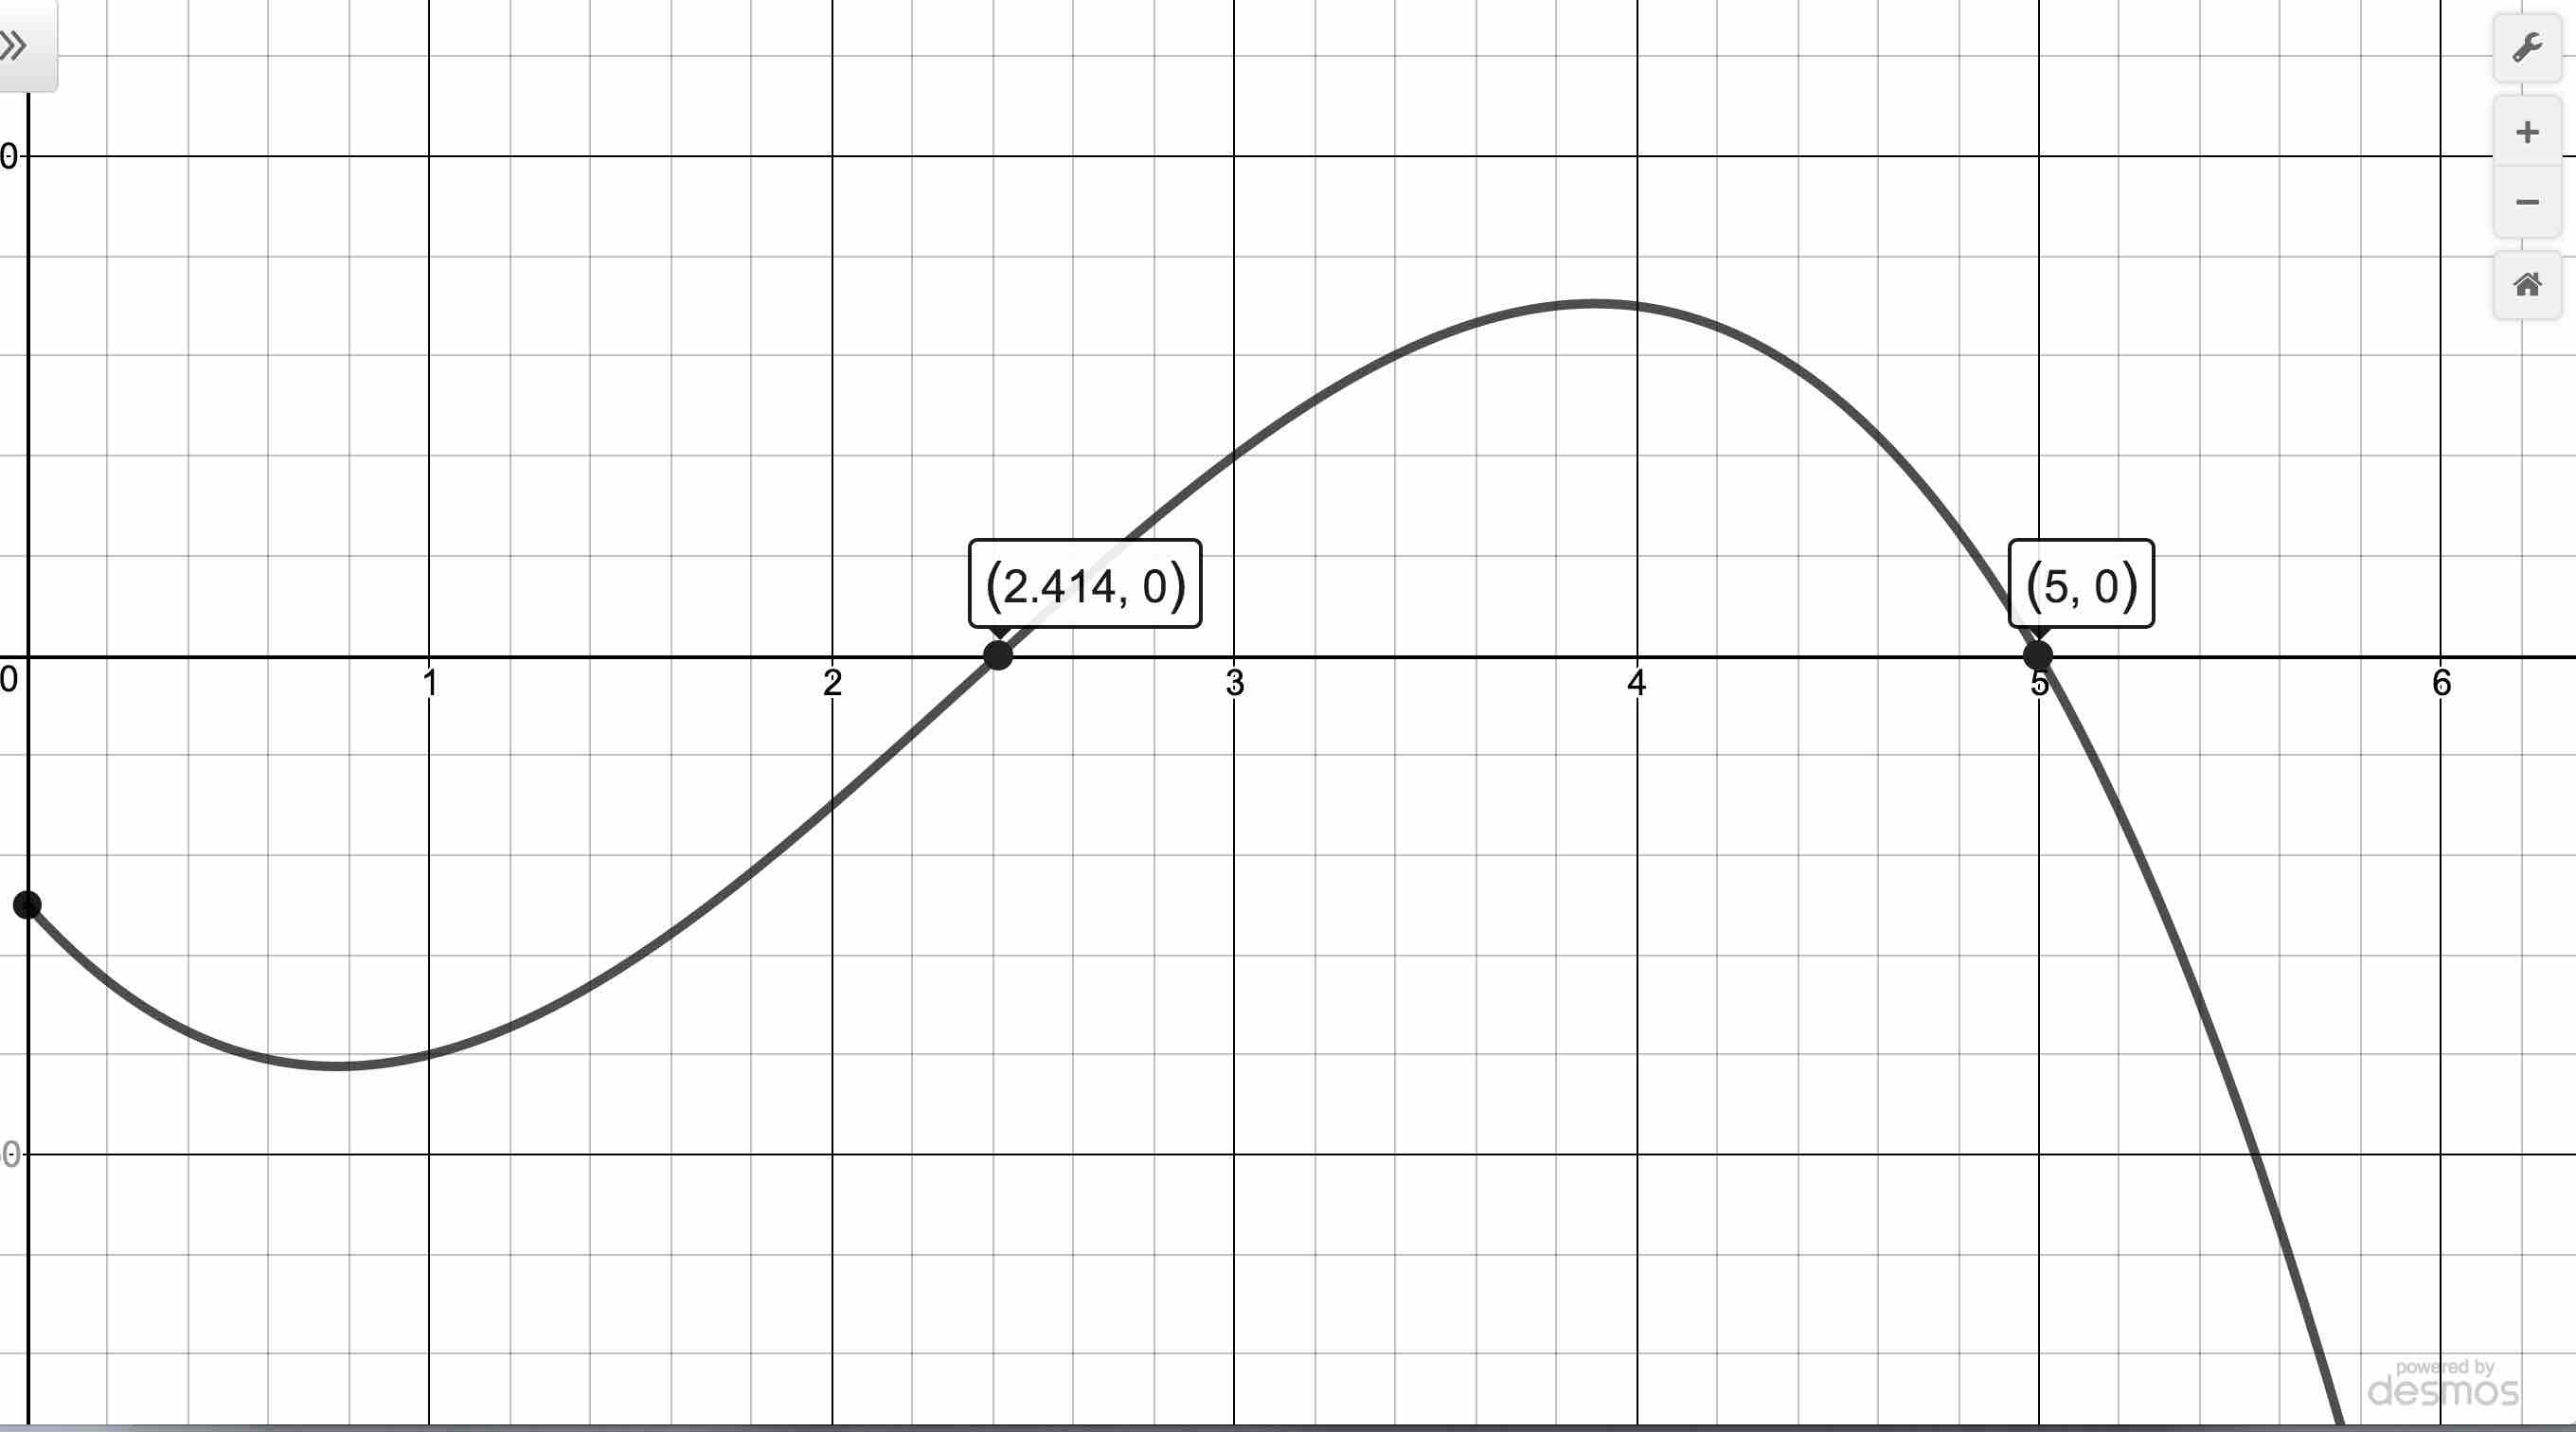
\includegraphics[width = 4in]{./RealZerosGraphics/RealZerosEx04.jpg}

\end{center}  

 \qed

\end{ex}


It would be a sin of omission if the authors left the reader with the impression that the theory in this section is compete in that given \textit{any} polynomial function, provided here are the tools to find all of its real zeros exactly.  The reality is this couldn't be further from the truth.  In general, no matter how many theorems you throw at a polynomial, it may well be impossible to express its zeros exactly.  The polynomial $f(x) = x^5-x-1$ is one such beast.\footnote{See this \href{http://en.wikipedia.org/wiki/Galois_theory}{\underline{page}}.}  According to Descartes' Rule of Signs, $f$ has exactly one positive real zero, and it could have two negative real zeros, or none at all.  The Rational Zeros Test gives us $\pm 1$ as rational zeros to try but neither of these work since $f(1) = f(-1) = -1$.  If we try the substitution technique we used in Example \ref{usubex}, we find $f(x)$ has three terms, but the exponent on the $x^5$ isn't exactly twice the exponent on $x$.  How could we go about approximating the positive zero?   We use the \index{Bisection Method} \textbf{Bisection Method}.  

\phantomsection
\label{bisectionmethod}

The first step in the Bisection Method is to find an interval on which $f$ changes sign.  We know $f(1) = -1$ and we find $f(2) = 29$.  By the Intermediate Value Theorem, we know that the zero of $f$ lies in the interval $[1,2]$.  Next, we `bisect' this interval by finding the midpoint,  $1.5$.  We compute  $f(1.5)\approx 5.09$.  Once again, the Intermediate Value Theorem guarantees our zero is between $1$ and $1.5$, since $f$ changes sign on this interval.  Now, we `bisect' the interval $[1,1.5]$ and find $f(1.25) \approx 0.80$, so now we have the zero between $1$ and $1.25$.  Bisecting $[1,1.25]$, we find $f(1.125) \approx -0.32$, which means the zero of $f$ is between $1.125$ and $1.25$.  We continue in this fashion until we have `sandwiched' the zero between two numbers whose digits agree to a desired amount.\footnote{We ask you to approximate this zero to three decimal places using the Bisection Method  in Exercise \ref{bisectionexercise}.} You can think of the Bisection Method as reversing the sign diagram process:  instead of finding the zeros and checking the sign of $f$ using test values, we are using test values to determine where the signs switch to find the zeros.  It is a slow and tedious, yet fool-proof, method for \textit{approximating} a real zero when the other analytical methods fail us.  


\newpage

\subsection{Exercises}

In Exercises \ref{prelimpolystufffirst} - \ref{prelimpolystufflast}, for the given polynomial:

\begin{itemize}
\item  Use Cauchy's Bound to find an interval containing all of the real zeros.
\item  Use the Rational Zeros Theorem to make a list of possible rational zeros.
\item  Use Descartes' Rule of Signs to list the possible number of positive and negative real zeros, counting multiplicities.
\end{itemize}


\begin{multicols}{2}
\begin{enumerate}

\item $f(x) = x^{3} - 2x^{2} - 5x + 6$ \label{prelimpolystufffirst}
\item $f(x) = x^{4} + 2x^{3} - 12x^{2} - 40x - 32$

\setcounter{HW}{\value{enumi}}
\end{enumerate}
\end{multicols}

\begin{multicols}{2}
\begin{enumerate}
\setcounter{enumi}{\value{HW}}

\item $p(z) = z^{4} - 9z^{2} - 4z + 12$
\item $p(z) = z^{3} + 4z^{2} - 11z + 6$

\setcounter{HW}{\value{enumi}}
\end{enumerate}
\end{multicols}

\begin{multicols}{2}
\begin{enumerate}
\setcounter{enumi}{\value{HW}}

\item $g(t) = t^{3} - 7t^{2} + t - 7$
\item $g(t) = -2t^{3} + 19t^{2} - 49t + 20$

\setcounter{HW}{\value{enumi}}
\end{enumerate}
\end{multicols}

\begin{multicols}{2}
\begin{enumerate}
\setcounter{enumi}{\value{HW}}

\item $f(x) = -17x^{3} + 5x^{2} + 34x - 10$
\item $f(x) = 36x^{4} - 12x^{3} - 11x^{2} + 2x + 1$

\setcounter{HW}{\value{enumi}}
\end{enumerate}
\end{multicols}

\begin{multicols}{2}
\begin{enumerate}
\setcounter{enumi}{\value{HW}}

\item $p(z) = 3z^{3} + 3z^{2} - 11z - 10$
\item $p(z) = 2z^4+z^3-7z^2-3z+3$ \label{prelimpolystufflast}


\setcounter{HW}{\value{enumi}}
\end{enumerate}
\end{multicols}


In Exercises \ref{findrealzerosexerfirst} - \ref{findrealzerosexerlast}, find the real zeros of the polynomial using the techniques specified by your instructor.  State the multiplicity of each real zero.


\begin{multicols}{2}
\begin{enumerate}
\setcounter{enumi}{\value{HW}}

\item $f(x) = x^{3} - 2x^{2} - 5x + 6$ \label{findrealzerosexerfirst}
\item $f(x) = x^{4} + 2x^{3} - 12x^{2} - 40x - 32$

\setcounter{HW}{\value{enumi}}
\end{enumerate}
\end{multicols}

\begin{multicols}{2}
\begin{enumerate}
\setcounter{enumi}{\value{HW}}

\item $p(z) = z^{4} - 9z^{2} - 4z + 12$
\item $p(z) = z^{3} + 4z^{2} - 11z + 6$

\setcounter{HW}{\value{enumi}}
\end{enumerate}
\end{multicols}

\begin{multicols}{2}
\begin{enumerate}
\setcounter{enumi}{\value{HW}}

\item $g(t) = t^{3} - 7t^{2} + t - 7$
\item $g(t) = -2t^{3} + 19t^{2} - 49t + 20$

\setcounter{HW}{\value{enumi}}
\end{enumerate}
\end{multicols}

\begin{multicols}{2}
\begin{enumerate}
\setcounter{enumi}{\value{HW}}

\item $f(x) = -17x^{3} + 5x^{2} + 34x - 10$
\item $f(x) = 36x^{4} - 12x^{3} - 11x^{2} + 2x + 1$

\setcounter{HW}{\value{enumi}}
\end{enumerate}
\end{multicols}

\begin{multicols}{2}
\begin{enumerate}
\setcounter{enumi}{\value{HW}}

\item $p(z) = 3z^{3} + 3z^{2} - 11z - 10$
\item $p(z) = 2z^4+z^3-7z^2-3z+3$

\setcounter{HW}{\value{enumi}}
\end{enumerate}
\end{multicols}

\begin{multicols}{2}
\begin{enumerate}
\setcounter{enumi}{\value{HW}}

\item $g(t) = 9t^{3} - 5t^{2} - t$
\item $g(t) = 6t^{4} - 5t^{3} - 9t^{2}$

\setcounter{HW}{\value{enumi}}
\end{enumerate}
\end{multicols}

\begin{multicols}{2}
\begin{enumerate}
\setcounter{enumi}{\value{HW}}

\item $f(x) = x^4+2x^2 - 15$
\item $f(x) = x^4-9x^2+14$

\setcounter{HW}{\value{enumi}}
\end{enumerate}
\end{multicols}

\begin{multicols}{2}
\begin{enumerate}
\setcounter{enumi}{\value{HW}}

\item $p(z) = 3z^4-14z^2-5$
\item $p(z) = 2z^4-7z^2+6$

\setcounter{HW}{\value{enumi}}
\end{enumerate}
\end{multicols}

\begin{multicols}{2}
\begin{enumerate}
\setcounter{enumi}{\value{HW}}

\item $g(t) = t^6-3t^3-10$
\item $g(t) = 2t^6-9t^3+10$

\setcounter{HW}{\value{enumi}}
\end{enumerate}
\end{multicols}

\begin{multicols}{2}
\begin{enumerate}
\setcounter{enumi}{\value{HW}}

\item $f(x) = x^5-2x^4-4x+8$
\item $f(x) = 2x^5+3x^4-18x-27$ \label{findrealzerosexerlast}

\setcounter{HW}{\value{enumi}}
\end{enumerate}
\end{multicols}

\pagebreak

In Exercises \ref{realzeroswcalcfirst} - \ref{realzeroswcalclast}, use your calculator,\footnote{You \textit{can} do these without your calculator, but it may test your mettle!} to help you find the real zeros of the polynomial.  State the multiplicity of each real zero.

\begin{enumerate}
\setcounter{enumi}{\value{HW}}

\item $f(x) = x^{5} - 60x^{3} - 80x^{2} + 960x + 2304$ \label{realzeroswcalcfirst}
\item $f(x) = 25x^{5} - 105x^{4} + 174x^{3} - 142x^{2} + 57x - 9$
\item $f(x) = 90x^{4} - 399x^{3} + 622x^{2} - 399x + 90$ \label{realzeroswcalclast}

\setcounter{HW}{\value{enumi}}
\end{enumerate}

\begin{enumerate}
\setcounter{enumi}{\value{HW}}

\item Find the real zeros of $f(x) = x^{3} - \frac{1}{12}x^{2} - \frac{7}{72}x + \frac{1}{72}$ by first finding a polynomial $q(x)$ with integer coefficients such that $q(x) = N \cdot f(x)$ for some integer $N$.  (Recall that the Rational Zeros Theorem required the polynomial in question to have integer coefficients.) Show that $f$ and $q$ have the same real zeros.

\setcounter{HW}{\value{enumi}}
\end{enumerate}

In Exercises \ref{polyequexerfirst} - \ref{polyequexerlast}, find the real solutions of the polynomial equation.  (See Example \ref{polyeqineqexample}.)

\begin{multicols}{2}
\begin{enumerate}
\setcounter{enumi}{\value{HW}}

\item  $9x^{3} = 5x^{2} + x$  \label{polyequexerfirst} 
\item $9x^{2}+5x^{3}= 6x^{4}$  

\setcounter{HW}{\value{enumi}}
\end{enumerate}
\end{multicols}

\begin{multicols}{2}
\begin{enumerate}
\setcounter{enumi}{\value{HW}}

\item $z^{3} + 6 = 2z^{2} + 5z$ 
\item $z^{4} + 2z^{3} = 12z^{2} + 40z + 32$ 

\setcounter{HW}{\value{enumi}}
\end{enumerate}
\end{multicols}


\begin{multicols}{2}
\begin{enumerate}
\setcounter{enumi}{\value{HW}}

\item $t^{3} - 7t^{2} = 7-t$ 
\item $2t^{3} = 19t^{2} - 49t + 20$ 

\setcounter{HW}{\value{enumi}}
\end{enumerate}
\end{multicols}

\begin{multicols}{2}
\begin{enumerate}
\setcounter{enumi}{\value{HW}}

\item $x^{3} + x^{2} = \dfrac{11x + 10}{3}$ 
\item $x^4+2x^2 = 15$ 


\setcounter{HW}{\value{enumi}}
\end{enumerate}
\end{multicols}

\begin{multicols}{2}
\begin{enumerate}
\setcounter{enumi}{\value{HW}}

\item $14z^{2}+5=3z^{4}$  

\item $2z^5+3z^4 = 18z + 27$ \label{polyequexerlast}  

\setcounter{HW}{\value{enumi}}
\end{enumerate}
\end{multicols}


In Exercises \ref{polyinequexerfirst} - \ref{polyinequexerlast}, solve the polynomial inequality and state your answer using interval notation.



\begin{multicols}{2}
\begin{enumerate}
\setcounter{enumi}{\value{HW}}

\item $-2x^{3} + 19x^{2} - 49x + 20 > 0$ \label{polyinequexerfirst}
\item $x^{4} - 9x^{2} \leq 4x - 12$

\setcounter{HW}{\value{enumi}}
\end{enumerate}
\end{multicols}

\begin{multicols}{2}
\begin{enumerate}
\setcounter{enumi}{\value{HW}}

\item $(z - 1)^{2} \geq 4$
\item $4z^3 \geq 3z+1$

\setcounter{HW}{\value{enumi}}
\end{enumerate}
\end{multicols}

\begin{multicols}{2}
\begin{enumerate}
\setcounter{enumi}{\value{HW}}

\item $t^4 \leq 16+4t-t^3$
\item $3t^2 + 2t < t^4$

\setcounter{HW}{\value{enumi}}
\end{enumerate}
\end{multicols}

\begin{multicols}{2}
\begin{enumerate}
\setcounter{enumi}{\value{HW}}

\item $\dfrac{x^3+2 x^2}{2} < x+2$
\item $\dfrac{x^3+20x}{8} \geq x^2 + 2$

\setcounter{HW}{\value{enumi}}
\end{enumerate}
\end{multicols}

\begin{multicols}{2}
\begin{enumerate}
\setcounter{enumi}{\value{HW}}

\item $2z^4>5z^2+3$
\item $z^6 + z^3 \geq 6$ \label{polyinequexerlast}

\setcounter{HW}{\value{enumi}}
\end{enumerate}
\end{multicols}


\newpage

In Exercises \ref{polyineqfromgraphfirst} - \ref{polyineqfromgraphlast}, use the the graph of the given polynomial function to  solve the stated inequality.

\begin{multicols}{2}
\begin{enumerate}
\setcounter{enumi}{\value{HW}}

\item  \label{polyineqfromgraphfirst} Solve $f(x) < 0$. 

\begin{mfpic}[10]{-7}{7}{-6}{6}
\axes
\tlabel[cc](7,-0.5){\scriptsize $x$}
\tlabel[cc](0.5,6){\scriptsize $y$}
\tlabel[cc](-4.5, 0.75){\scriptsize $(-6,0)$}
\tlabel[cc](5, 0.75){\scriptsize $(6,0)$}
\tlabel[cc](1, 0.75){\scriptsize $(0,0)$}
\point[4pt]{(-6,0),(0,0),(6,0)}
\xmarks{-6 step 1 until 6}
\tiny
\tlpointsep{4pt}
\axislabels {x}{{$-6 \hspace{6pt}$} -6, {$-5 \hspace{6pt}$} -5, {$-4 \hspace{6pt}$} -4, {$-3 \hspace{6pt}$} -3, {$-2 \hspace{6pt}$} -2, {$-1 \hspace{6pt}$} -1, {$1$} 1, {$2$} 2, {$3$} 3, {$4$} 4, {$5$} 5, {$6$} 6}
\normalsize
\penwd{1.25pt}
\arrow \reverse \arrow \function{-7,7,0.1}{((x**3) - 36*x)/20}
\tcaption{$y = f(x)$}
\end{mfpic}

\vfill

\columnbreak

\item Solve $g(t) > 0$.


\begin{mfpic}[20][20]{-3}{3}{-2}{5}
\axes
\tlabel[cc](3,-0.5){\scriptsize $t$}
\tlabel[cc](0.25,5){\scriptsize $y$}
\tlabel[cc](-1.75, 0.3){\scriptsize $(-2,0)$}
\tlabel[cc](0.5, 0.3){\scriptsize $(0,0)$}
\point[4pt]{(-2,0), (0,0)}
\xmarks{-2,-1, 1, 2}
\tiny
\tlpointsep{4pt}
\axislabels {x}{{$-2 \hspace{6pt}$} -2, {$-1 \hspace{6pt}$} -1, {$1$} 1, {$2$} 2}
\normalsize
\penwd{1.25pt}
\arrow \reverse \arrow \function{-3,0.3,0.1}{x*((x + 2)**3)}
\tcaption{$y = g(t)$ }
\end{mfpic}


\setcounter{HW}{\value{enumi}}
\end{enumerate}
\end{multicols}


\begin{multicols}{2}
\begin{enumerate}
\setcounter{enumi}{\value{HW}}

\item  Solve $p(z) \geq 0$ 

\begin{mfpic}[20][10]{-3}{3}{-4}{4}
\axes
\tlabel[cc](3,-0.5){\scriptsize $z$}
\tlabel[cc](0.25,4){\scriptsize $y$}
\tlabel[cc](-2, 0.75){\scriptsize $(-1,0)$}
\tlabel[cc](2, 0.75){\scriptsize $(2,0)$}
\point[4pt]{(2,0), (-1,0)}
\xmarks{-2,-1,1,2}
\tiny
\tlpointsep{4pt}
\axislabels {x}{{$-2 \hspace{6pt}$} -2, {$-1 \hspace{6pt}$} -1, {$1$} 1, {$2$} 2}
\normalsize
\penwd{1.25pt}
\arrow \reverse \arrow \function{-1.70,3.45,0.1}{(-0.4)*((x-2)**2)*(x+1)}
\tcaption{$y = p(z)$}
\end{mfpic}

\vfill

\columnbreak




\item Solve $f(x) < 0$.


\begin{mfpic}[20][10]{-2}{4}{-4}{4}
\axes
\tlabel[cc](4,-0.5){\scriptsize $x$}
\tlabel[cc](0.25,4){\scriptsize $y$}
\tlabel[cc](-0.75, 0.75){\scriptsize $\left(-\frac{1}{2},0 \right)$}
\tlabel[cc](2.5, 0.75){\scriptsize $(3,0)$}
\point[4pt]{(-0.5,0), (3,0)}
\xmarks{-1,1,2,3}
\tiny
\tlpointsep{4pt}
\axislabels {x}{ {$1$} 1, {$2$} 2, {$3$} 3}
\normalsize
\penwd{1.25pt}
\arrow \reverse \arrow \function{-1.5,3.3,0.1}{(0.5)*((x+0.5)**2)*(x-3)}
\tcaption{$y = f(x)$ }
\end{mfpic}

\setcounter{HW}{\value{enumi}}
\end{enumerate}
\end{multicols}


\begin{multicols}{2}
\begin{enumerate}
\setcounter{enumi}{\value{HW}}

\item Solve $F(s) \leq 0$.  

\begin{mfpic}[20][10]{-3}{3}{-5}{5}
\axes
\tlabel[cc](3,-0.5){\scriptsize $s$}
\tlabel[cc](0.25,5){\scriptsize $y$}
\tlabel[cc](-2, -0.75){\scriptsize $(-2,0)$}
\tlabel[cc](0.5, 0.75){\scriptsize $(0,0)$}
\point[4pt]{(-2,0), (0,0)}
\xmarks{-2,-1,1,2}
\tiny
\tlpointsep{4pt}
\axislabels {x}{ {$1$} 1, {$2$} 2}
\normalsize
\penwd{1.25pt}
\arrow \reverse \arrow \function{-3,0.65,0.1}{0-x*((x + 2)**2)}
\tcaption{$y = F(s)$}
\end{mfpic}



\vfill

\columnbreak

\item \label{polyineqfromgraphlast} Solve $G(t) \geq 0$.

\begin{mfpic}[20][10]{-3}{3}{-5}{5}
\axes
\tlabel[cc](-2, 0.75){\scriptsize $(-2,0)$}
\tlabel[cc](0.5, -0.75){\scriptsize $(0,0)$}
\tlabel[cc](3,-0.5){\scriptsize $t$}
\tlabel[cc](0.25,5){\scriptsize $y$}
\point[4pt]{(-2,0), (0,0)}
\xmarks{-2,-1,1,2}
\tiny
\tlpointsep{4pt}
\axislabels {x}{  {$2$} 2}
\normalsize
\penwd{1.25pt}
\arrow \reverse \arrow \function{-2.45,0.85,0.1}{(x**3)*((x + 2)**2)}
\tcaption{$y = G(t)$}
\end{mfpic}


\setcounter{HW}{\value{enumi}}
\end{enumerate}
\end{multicols}



\begin{enumerate}
\setcounter{enumi}{\value{HW}}

\item Use the Intermediate Value Theorem, Theorem \ref{IVT} to prove that $f(x) = x^{3} - 9x + 5$ has a real zero in each of the following intervals: $[-4, -3], [0, 1]$ and $[2, 3]$.

\item  Use the concepts of End Behavior and the Intermediate Value Theorem to prove any odd-degree polynomial function with real number coefficients has at least one real zero.

\item Find an even-degree polynomial function with real number coefficients which has no real zeros.

\item  \label{bisectionexercise} Continue  the Bisection Method as introduced on  \pageref{bisectionmethod} to approximate the real zero of $f(x) = x^5-x-1$ to three decimal places.

\item  \label{sqrt2isirrationalexercise} In this exercise, we prove $\sqrt{2}$ is an irrational number and approximate its value.  Let $f(x) = x^2-2$.

\begin{enumerate} 

\item Use Decartes' Rule of Signs to prove $f$ has exactly one positive real zero.

 \item Use the Intermediate Value Theorem to prove $f$ has a zero in $[1,2]$.

\item \label{sqrt2isirrationalexercise}  Use the Rational Zeros Theorem to prove $f$ has no rational zeros.

\item  Use the Bisection Method (see  \pageref{bisectionmethod}) to approximate the zero of $f$ on $[1,2]$ to three decimal places.

\end{enumerate}

\item  Generalize the argument given in Exercise \ref{sqrt2isirrationalexercise} to prove:

\begin{enumerate}

\item If $N$ is not the perfect square of an integer, then $\sqrt{N}$ is irrational. (HINT: Consider $f(x) = x^2-N$.)

\item  For natural numbers $n \geq 2$, if $N$ is not the perfect $n^{\text{th}}$ power of an integer, then $\sqrt[n]{N}$ is irrational. (HINT: Consider $f(x) = x^n-N$.)

\end{enumerate}

\item  In Example \ref{boxnotopex} in Section \ref{GraphsofPolynomials}, a box with no top is constructed from a $10$ inch $\times$ $12$ inch piece of cardboard by cutting out congruent squares from each corner of the cardboard and then folding the resulting tabs.  We determined the volume of that box (in cubic inches) is given by  the function$V(x) = 4x^3-44x^2+120x$, where $x$ denotes the length of the side of the square which is removed from each corner (in inches), $0 < x < 5$.  Solve the inequality $V(x) \geq 80$ analytically and interpret your answer in the context of that example.

\item  From Exercise \ref{newportaboycost} in Section \ref{GraphsofPolynomials}, $C(x) = .03x^{3} - 4.5x^{2} + 225x + 250$, for $x \geq 0$ models the cost, in dollars, to produce $x$ PortaBoy game systems. If the production budget is $\$5000$, find the number of game systems which can be produced and still remain under budget.

\item Let $f(x) = 5x^{7} - 33x^{6} + 3x^{5} - 71x^{4} - 597x^{3} + 2097x^{2} - 1971x + 567$.  With the help of your classmates, find the $x$- and $y$- intercepts of the graph of $f$.  Find the intervals on which the function is increasing, the intervals on which it is decreasing and the local extrema.  Sketch the graph of $f$, using more than one picture if necessary to show all of the important features of the graph.  

\item With the help of your classmates, create a list of five polynomials with different degrees whose real zeros cannot be found using any of the techniques in this section.

\setcounter{HW}{\value{enumi}}
\end{enumerate}
 



\newpage

\subsection{Answers}

\begin{enumerate}

\item For $f(x) = x^{3} - 2x^{2} - 5x + 6$
\begin{itemize}
\item  All of the real zeros lie in the interval $[-7,7]$
\item  Possible rational zeros are $\pm 1$, $\pm 2$, $\pm 3$, $\pm 6$
\item  There are 2 or 0 positive real zeros;  there is 1 negative real zero
\end{itemize}

\item For  $f(x) = x^{4} + 2x^{3} - 12x^{2} - 40x - 32$
\begin{itemize}
\item  All of the real zeros lie in the interval $[-41,41]$
\item  Possible rational zeros are $\pm 1$, $\pm 2$, $\pm 4$, $\pm 8$, $\pm 16$, $\pm 32$
\item  There is 1 positive real zero;  there are 3 or 1 negative real zeros
\end{itemize}

\item For  $p(z) = z^{4} - 9z^{2} - 4z + 12$
\begin{itemize}
\item  All of the real zeros lie in the interval $[-13,13]$
\item  Possible rational zeros are $\pm 1$, $\pm 2$, $\pm 3$, $\pm 4$, $\pm 6$, $\pm 12$
\item  There are 2 or 0 positive real zeros;  there are 2 or 0 negative real zeros
\end{itemize}

\item For  $p(z) = z^{3} + 4z^{2} - 11z + 6$
\begin{itemize}
\item  All of the real zeros lie in the interval $[-12,12]$
\item  Possible rational zeros are $\pm 1$, $\pm 2$, $\pm 3$, $\pm 6$
\item  There are 2 or 0 positive real zeros;  there is 1 negative real zero
\end{itemize}

\item For   $g(t) = t^{3} - 7t^{2} + t - 7$
\begin{itemize}
\item  All of the real zeros lie in the interval $[-8,8]$
\item  Possible rational zeros are $\pm 1$, $\pm 7$
\item  There are 3 or 1 positive real zeros;  there are no negative real zeros
\end{itemize}

\item For   $g(t) = -2t^{3} + 19t^{2} - 49t + 20$
\begin{itemize}
\item  All of the real zeros lie in the interval $\left[-\frac{51}{2},\frac{51}{2} \right]$
\item  Possible rational zeros are  $\pm \frac{1}{2}$, $\pm 1$, $\pm 2$, $\pm \frac{5}{2}$, $\pm 4$, $\pm 5$, $\pm 10$, $\pm 20$ 
\item  There are 3 or 1 positive real zeros;  there are no negative real zeros
\end{itemize}

\item For   $f(x) = -17x^{3} + 5x^{2} + 34x - 10$
\begin{itemize}
\item  All of the real zeros lie in the interval $[-3,3]$
\item  Possible rational zeros are $\pm \frac{1}{17}$, $\pm \frac{2}{17}$, $\pm \frac{5}{17}$, $\pm \frac{10}{17}$, $\pm 1$, $\pm 2$, $\pm 5$, $\pm 10$
\item  There are 2 or 0 positive real zeros;  there is 1 negative real zero
\end{itemize}

\item For   $f(x) = 36x^{4} - 12x^{3} - 11x^{2} + 2x + 1$
\begin{itemize}
\item  All of the real zeros lie in the interval $\left[-\frac{4}{3},\frac{4}{3}\right]$
\item  Possible rational zeros are $\pm \frac{1}{36}$, $\pm \frac{1}{18}$, $\pm \frac{1}{12}$, $\pm \frac{1}{9}$, $\pm \frac{1}{6}$, $\pm \frac{1}{4}$, $\pm \frac{1}{3}$, $\pm \frac{1}{2}$, $\pm 1$
\item  There are 2 or 0 positive real zeros;  there are 2 or 0 negative real zeros
\end{itemize}

\item For   $p(z) = 3z^{3} + 3z^{2} - 11z - 10$
\begin{itemize}
\item  All of the real zeros lie in the interval $\left[-\frac{14}{3},\frac{14}{3}\right]$
\item  Possible rational zeros are $\pm \frac{1}{3}$, $\pm \frac{2}{3}$, $\pm \frac{5}{3}$, $\pm \frac{10}{3}$, $\pm 1$, $\pm 2$, $\pm 5$, $\pm 10$
\item  There is 1 positive real zero;  there are 2 or 0 negative real zeros
\end{itemize}

\item For   $p(z) = 2z^4+z^3-7z^2-3z+3$
\begin{itemize}
\item  All of the real zeros lie in the interval $\left[-\frac{9}{2},\frac{9}{2}\right]$
\item  Possible rational zeros are  $\pm \frac{1}{2}$, $\pm 1$,  $\pm \frac{3}{2}$, $\pm 3$
\item  There are 2 or 0 positive real zeros;  there are 2 or 0 negative real zeros
\end{itemize}


\item $f(x) = x^{3} - 2x^{2} - 5x + 6$ \\ $x = -2$, $x = 1$, $x = 3$ (each has mult. 1)
\item $f(x) = x^{4} + 2x^{3} - 12x^{2} - 40x - 32$ \\ $x = -2$ (mult. 3), $x = 4$ (mult. 1)


\item $p(z) = z^{4} - 9z^{2} - 4z + 12$ \\ $z = -2$ (mult. 2), $z = 1$ (mult. 1), $z = 3$ (mult. 1)
\item $p(z) = z^{3} + 4z^{2} - 11z + 6$ \\ $z = -6$ (mult. 1), $z = 1$ (mult. 2)

\item $g(t) = t^{3} - 7t^{2} + t - 7$ \\ $t = 7$ (mult. 1)
\item $g(t) = -2t^{3} + 19t^{2} - 49t + 20$ \\ $t = \frac{1}{2}$, $t = 4$, $t = 5$ (each has mult. 1)

\item $f(x) = -17x^{3} + 5x^{2} + 34x - 10$ \\ $x = \frac{5}{17}$, $x = \pm \sqrt{2}$ (each has mult. 1)
\item $f(x) = 36x^{4} - 12x^{3} - 11x^{2} + 2x + 1$ \\ $x = \frac{1}{2}$ (mult. 2), $x = -\frac{1}{3}$ (mult. 2)

\item $p(z) = 3z^{3} + 3z^{2} - 11z - 10$ \\ $z = -2$, $z = \frac{3 \pm \sqrt{69}}{6}$ (each has mult. 1)
\item $p(z) = 2z^4+z^3-7z^2-3z+3$ \\ $z = -1$, $z = \frac{1}{2}$, $z=\pm \sqrt{3}$ (each mult. 1)

\item $g(t) = 9t^{3} - 5t^{2} - t$ \\ $t = 0$, $t = \frac{5 \pm \sqrt{61}}{18}$ (each has mult. 1)
\item $g(t) = 6t^{4} - 5t^{3} - 9t^{2}$ \\ $t = 0$ (mult. 2), $t = \frac{5 \pm \sqrt{241}}{12}$ (each has mult. 1)

\item $f(x) = x^4+2x^2 - 15$ \\ $x = \pm \sqrt{3}$ (each has mult. 1)
\item $f(x) = x^4-9x^2+14$ \\ $x = \pm \sqrt{2}$, $x = \pm \sqrt{7}$ (each has mult. 1)

\item $p(z) = 3z^4-14z^2-5$ \\ $z = \pm \sqrt{5}$ (each has mult. 1)
\item $p(z)  = 2z^4-7z^2+6$ \\  $z = \pm \frac{\sqrt{6}}{2}$, $z = \pm \sqrt{2}$ (each has mult. 1)

\item $g(t) = t^6-3t^3-10$ \\ $t = \sqrt[3]{-2} = -\sqrt[3]{2}$, $t = \sqrt[3]{5}$ (each has mult. 1)
\item $g(t) = 2t^6-9t^3+10$ \\ $t =\frac{\sqrt[3]{20}}{2} $, $t = \sqrt[3]{2}$ (each has mult. 1)


\item $f(x) = x^5-2x^4-4x+8$ \\ $x = 2$, $x = \pm \sqrt{2}$ (each has mult. 1)
\item $f(x) = 2x^5+3x^4-18x-27$ \\ $x = -\frac{3}{2}$, $x = \pm \sqrt{3}$ (each has mult. 1)

\item $f(x) = x^{5} - 60x^{3} - 80x^{2} + 960x + 2304 $ \\ $x = -4$ (mult. 3), $x = 6$ (mult. 2)


\item $f(x) = 25x^{5} - 105x^{4} + 174x^{3} - 142x^{2} + 57x - 9$ \\ $x = \frac{3}{5}$ (mult. 2), $x = 1$ (mult. 3)

\item $f(x) = 90x^{4} - 399x^{3} + 622x^{2} - 399x + 90$ \\ $x = \frac{2}{3}$, $x = \frac{3}{2}$, $x = \frac{5}{3}$, $x = \frac{3}{5}$ (each has mult. 1)


\item We choose $q(x) = 72x^{3} - 6x^{2} - 7x + 1 = 72 \cdot f(x)$.  Clearly $f(x) = 0$ if and only if $q(x) = 0$ so they have the same real zeros.  In this case, $x = -\frac{1}{3}, \; x = \frac{1}{6} \;$ and $x = \frac{1}{4}$ are the real zeros of both $f$ and $q$.


\setcounter{HW}{\value{enumi}}
\end{enumerate}


\begin{multicols}{2}
\begin{enumerate}
\setcounter{enumi}{\value{HW}}

\item  $x = 0, \frac{5\pm \sqrt{61}}{18}$
\item  $x = 0, \frac{5 \pm \sqrt{241}}{12}$

\setcounter{HW}{\value{enumi}}
\end{enumerate}
\end{multicols}

\begin{multicols}{2}
\begin{enumerate}
\setcounter{enumi}{\value{HW}}

\item $z = -2,1,3$
\item $z=-2,4$

\setcounter{HW}{\value{enumi}}
\end{enumerate}
\end{multicols}


\begin{multicols}{2}
\begin{enumerate}
\setcounter{enumi}{\value{HW}}

\item $t=7$
\item $t = \frac{1}{2}, 4, 5$

\setcounter{HW}{\value{enumi}}
\end{enumerate}
\end{multicols}

\begin{multicols}{2}
\begin{enumerate}
\setcounter{enumi}{\value{HW}}

\item $x = -2, \frac{3 \pm \sqrt{69}}{6}$

\item $x = \pm \sqrt{3}$


\setcounter{HW}{\value{enumi}}
\end{enumerate}
\end{multicols}

\begin{multicols}{2}
\begin{enumerate}
\setcounter{enumi}{\value{HW}}

\item $z = \pm \sqrt{5}$

\item $z = -\frac{3}{2}, \pm \sqrt{3}$

\setcounter{HW}{\value{enumi}}
\end{enumerate}
\end{multicols}



\begin{multicols}{2}
\begin{enumerate}
\setcounter{enumi}{\value{HW}}

\item $(-\infty, \frac{1}{2}) \cup (4, 5)$
\item $\{-2\} \cup [1, 3]$

\setcounter{HW}{\value{enumi}}
\end{enumerate}
\end{multicols}

\begin{multicols}{2}
\begin{enumerate}
\setcounter{enumi}{\value{HW}}

\item $(-\infty, -1] \cup [3, \infty)$

\item $\left\{ -\dfrac{1}{2} \right\} \cup [1, \infty)$

\setcounter{HW}{\value{enumi}}
\end{enumerate}
\end{multicols}

\begin{multicols}{2}
\begin{enumerate}
\setcounter{enumi}{\value{HW}}

\item $[-2,2]$
\item $\left(-\infty, -1 \right) \cup \left(-1, 0 \right) \cup (2, \infty)$

\setcounter{HW}{\value{enumi}}
\end{enumerate}
\end{multicols}

\begin{multicols}{2}
\begin{enumerate}
\setcounter{enumi}{\value{HW}}


\item $(-\infty, -2) \cup \left(-\sqrt{2}, \sqrt{2} \right)$
\item $\{2 \} \cup [4,\infty)$

\setcounter{HW}{\value{enumi}}
\end{enumerate}
\end{multicols}

\begin{multicols}{2}
\begin{enumerate}
\setcounter{enumi}{\value{HW}}


\item $(-\infty, -\sqrt{3}) \cup (\sqrt{3}, \infty)$
\item $(-\infty, -\sqrt[3]{3}\,) \cup (\sqrt[3]{2}, \infty)$

\setcounter{HW}{\value{enumi}}
\end{enumerate}
\end{multicols}

\begin{multicols}{2}
\begin{enumerate}
\setcounter{enumi}{\value{HW}}

\item $f(x) < 0$ on $(-\infty, -6) \cup (0, 6)$

\item $g(t) > 0$ on $(-\infty, -2) \cup (0, \infty)$

\setcounter{HW}{\value{enumi}}
\end{enumerate}
\end{multicols}

\begin{multicols}{2}
\begin{enumerate}
\setcounter{enumi}{\value{HW}}

\item $p(z) \geq 0$ on $(-\infty, -1] \cup \{ 2\}$

\item $f(x) < 0$ on $\left( -\infty, -\frac{1}{2} \right) \cup \left(-\frac{1}{2}, 3 \right)$

\setcounter{HW}{\value{enumi}}
\end{enumerate}
\end{multicols}

\begin{multicols}{2}
\begin{enumerate}
\setcounter{enumi}{\value{HW}}

\item $F(s) \leq 0$ on $\{-2\} \cup [0, \infty)$

\item $G(t) \geq 0$ on $\{-2\} \cup [0, \infty)$

\setcounter{HW}{\value{enumi}}
\end{enumerate}
\end{multicols}


\begin{enumerate}
\setcounter{enumi}{\value{HW}}

\item Since $f(-4)=-23,\; f(-3)=5,\; f(0)=5,\; f(1)=-3,\; f(2)=-5\;$ and $f(3)=5$ the Intermediate Value Theorem gives that $f(x) = x^{3} - 9x + 5$ has real zeros in the intervals $[-4, -3], [0, 1]$ and $[2, 3]$. 


\item  An odd degree polynomial  function $f$ has `mismatched' end behavior.  That is, the end behavior of $f(x)$ is either:   $x \rightarrow -\infty$, $f(x) \rightarrow -\infty$ and as $x \rightarrow \infty$, $f(x) \rightarrow \infty$  or as  $x \rightarrow -\infty$, $f(x) \rightarrow \infty$ and as $x \rightarrow \infty$, $f(x) \rightarrow -\infty$.  This means at some point, $f(x) > 0$ and at some other point $f(x) < 0$.  The Intermediate Value Theorem guarantees at least one place where $f(x) = 0$.

\item  The function $f(x) = x^2+1$ has no real zeros.

\item  $x \approx 1.167$.

\item  \begin{enumerate} 

\item  $f(x)$ has only one variation in sign, so the result follows from Descartes' Rule of Signs.

 \item $f(1) = -1<0$ and $f(2) = 2>0$ so the Intermediate Value Theorem promises a zero in $[1,2]$.

\item The Rational Zeros Theorem gives the only possible rational zeros of $f$ are $\pm 1$ and $\pm 2$.  Since $f(\pm 1) = -1$ and $f(\pm 2) = 2$, $f$ has no rational zeros.  

\item  The zero of $f$ is $\sqrt{2} \approx 1.414$. 

\end{enumerate}

\item  $V(x) \geq 80$ on $[1,5-\sqrt{5}] \cup [5+\sqrt{5}, \infty)$.  Only the portion $[1,5-\sqrt{5}]$ lies in the applied domain, however.   In the context of the problem, this says for the volume of the box to be at least 80 cubic inches, the square removed from each corner needs to have a side length of at least 1 inch, but no more than $5-\sqrt{5} \approx 2.76$ inches.

\item $C(x) \leq 5000$ on (approximately) $(-\infty, 82.18]$.  The portion of this which lies in the applied domain is $(0,82.18]$.  Since $x$ represents the number of game systems, we check $C(82) = 4983.04$ and $C(83) = 5078.11$, so to remain within the production budget, anywhere between $1$ and $82$ game systems can be produced.


\setcounter{HW}{\value{enumi}}
\end{enumerate}


\closegraphsfile

\newpage

\section{Complex Zeros and the Fundamental Theorem of Algebra}

\mfpicnumber{1}

\opengraphsfile{ComplexZeros}

\setcounter{footnote}{0}

\label{ComplexZeros}

In Section \ref{RealZeros}, we were focused on finding the real zeros of a polynomial function.  In this section, we expand our horizons and look for the non-real zeros as well. By `non-real' here we mean we will be discussing `imaginary,' and, more generally, `complex' numbers.  Even though the monikers `non-real' and `imaginary' suggests these numbers play no role in `real' world applications, we assure you that electrical engineers live a `complex' life and these numbers are invaluable to them.\footnote{Even a cursory web search for `use of imaginary numbers in electrical engineering' provides a wealth of source material - enough to convince anyone of their importance to the field (pun intended.)  Most of it, however, requires more electrical background than the authors feel comfortable including in the text.  Be aware, however, that in electrical applications, the letter $j$ is used to represent $\sqrt{-1}$ since the letter $i$ is reserved for current.}  That being said, our main use of complex numbers in this section is to present some powerful structure theorems for polynomial functions (this is, after all, a math book!)  For a detailed review of the Complex Number system, we refer the reader to Section \ref{AppCmpNums}.  For us, it suffices to review the basic vocabulary.  

\colorbox{ResultColor}{\bbm

\begin{itemize}
 
\item The imaginary unit $i = \sqrt{-1}$ satisfies the two following properties

\begin{enumerate}

\item  $i^2 = -1$

\item  If $c$ is a real number with $c \geq 0$ then $\sqrt{-c} = i \sqrt{c}$

\end{enumerate}

\item The \textbf{complex numbers} are the set of numbers $\mathbb{C} = \{ a + bi \, | \, a, b \in \mathbb{R} \}$

\item  Given a complex number $z = a+bi$, the \textbf{complex conjugate} of $z$, $\overline{z}  = \overline{a+bi} = a - bi$.

\end{itemize}

\ebm}

Note that every real number is a complex number, that is $\mathbb{R} \subseteq \mathbb{C}$.  To see this, take your favorite real number, say $117$.  We may write $117 = 117 + 0 i$ which puts in the form $a + bi$.  Hence, we we speak of the `complex zeros' of a polynomial function, we are talking about not just the non-real, but also the real zeros.

Complex numbers, by their very definition, are two dimensional creatures.  To see this, we may identify a complex number $z = a+bi$ with the point in the Cartesian plane $(a,b)$. The horizontal axis is called the `real' axis since points here have the form $(a,0)$ which corresponds to numbers of the form $z = a + 0i = a$ which are the real numbers. The vertical axis is called the `imaginary' axis since points here are of the form $(0,b)$ which correspond to numbers of the form $z = 0+bi = bi$,  the so-called `purely imaginary' numbers.  Below we plot some complex numbers on this so-called  `Complex Plane.'  Plotting a set of complex numbers this way is called an \href{https://en.wikipedia.org/wiki/Complex_plane}{\underline{Argand Diagram}}, and opens up a wealth of opportunities to explore many algebraic properties of complex numbers geometrically. For example, complex conjugation amounts to a reflection about the real axis, and multiplication by $i$ amounts to a $90^{\circ}$ rotation.\footnote{See Exercises \ref{cmpgeoalgexfirst} - \ref{cmpgeoalgexlast}.}  While we won't have much use for the Complex Plane in this section, it is worth introducing this concept now, if, for no other reason, it gives the reader a sense of the vastness of the complex number system and the role of the real numbers in it.

\begin{center}

\begin{mfpic}[15]{-5}{5}{-5}{5}
\axes
\tlabel[cl](5,-0.5){\scriptsize Real Axis}
\tlabel[cl](0.5,5){\scriptsize Imaginary Axis}
\xmarks{-4,-3,-2,-1,1,2,3,4}
\ymarks{-4,-3,-2,-1,1,2,3,4}
\point[3pt]{(0,0),(3,0), (-4,2), (0,-3)}
\tlabel[cc](-4,2.5){\scriptsize $(-4,2) \longleftrightarrow z = -4+2i$}
\tlabel[cl](0.25,-3){\scriptsize $(0,-3) \longleftrightarrow z = -3i$}
\tlabel[cc](3,0.5){\scriptsize $(3,0) \longleftrightarrow z = 3$}
\tlabel[cc](0.25,-0.35){\scriptsize $0$}
\tlpointsep{5pt}
\scriptsize
\tcaption{\scriptsize The Complex Plane}
\axislabels {x}{{$-4 \hspace{7pt}$} -4, {$-3 \hspace{7pt} $} -3, {$-2\hspace{7pt} $} -2, {$-1 \hspace{7pt}$} -1, {$1$} 1, {$2$} 2, {$3$} 3, {$4$} 4}
\axislabels {y}{{$-4i$} -4, {$-3i$} -3, {$-2i$} -2, {$-i$} -1, {$i$} 1, {$2i$} 2, {$3i$} 3, {$4i$} 4}
\normalsize
\end{mfpic}

\end{center}




Returning to zeros of polynomials, suppose we wish to find the zeros of $f(x) = x^2-2x+5$.  To solve the equation $x^2-2x+5 = 0$, we note that the quadratic doesn't factor nicely, so we resort to the Quadratic Formula, Equation \ref{quadraticformulafunction} and obtain \[ x = \dfrac{-(-2) \pm \sqrt{(-2)^2-4(1)(5)}}{2(1)} = \dfrac{2 \pm \sqrt{-16}}{2} = \dfrac{2 \pm 4i}{2} = 1 \pm 2i.\] Two things are important to note.  First, the zeros $1+2i$ and $1-2i$ are complex conjugates.  If ever we obtain non-real zeros to a quadratic function with \textit{real number} coefficients, the zeros  will be a complex conjugate pair. (Do you see why?)  

We could ask if all of the theory from Section\ref{Polydivision} holds for non-real zeros, in particular the division algorithm and the Remainder and Factor Theorems.  The answer is `yes.'  

\[\begin{array}{rrrr}
1+2i \, \, \vline & 1 & -2 & 5 \\

  & \downarrow   &  1+2i  &  -5 \\ \hhline{~---} 
  
  & 1 & -1+2i &  \fbox{$0$}   \\

\end{array}\]


Indeed, the above shows $x^2-2x+5  = (x-[1+2i])(x-1+2i)= (x-[1+2i])(x-[1-2i])$ which demonstrates both  $(x-[1+2i])$ and  $(x-[1-2i])$ are factors of $x^2-2x+5$.\footnote{It is a good review of the algebra of complex numbers to start with  $(x-[1+2i])(x-[1-2i])$, perform the indicated operations, and simplify the result to $x^2-2x+5$.  See part 6 of  Example \ref{complexzeroex1}  in Section  \ref{AppCmpNums}.}


 But how do we know if a general polynomial has any complex zeros at all?  We have many examples of polynomials with no real zeros.  Can there be polynomials with no zeros whatsoever?  The answer to that last question is ``No.'' and the theorem which provides that answer is \index{Fundamental Theorem of Algebra} The Fundamental Theorem of Algebra.



\colorbox{ResultColor}{\bbm
\begin{thm} \label{ftoa} \textbf{The Fundamental Theorem of Algebra:}  Suppose $f$ is a polynomial function with complex number coefficients of degree $n \geq 1$, then $f$ has at least one complex zero.

\end{thm}
\ebm}



The Fundamental Theorem of Algebra is an example of an `existence' theorem in Mathematics.  Like the Intermediate Value Theorem, Theorem \ref{IVT}, the Fundamental Theorem of Algebra  guarantees the existence of at least one zero, but gives us no algorithm to use in finding it.  In fact, as we mentioned in Section \ref{RealZeros}, there are polynomials whose real zeros, though they exist, cannot be expressed using the `usual' combinations of arithmetic symbols, and must be approximated.  It took mathematicians literally hundreds of years to prove the theorem in its full generality,\footnote{So if its profound nature and beautiful subtlety escape you, no worries!} and some of that history is recorded \href{http://en.wikipedia.org/wiki/Fundamental_theorem_of_algebra}{\underline{here}}.  Note that the Fundamental Theorem of Algebra  applies to not only polynomial functions with real coefficients, but to those with complex number coefficients as well.  



Suppose  $f$ is a polynomial function of degree $n \geq 1$.  The Fundamental Theorem of Algebra guarantees us at least one complex zero, $z_{\mbox{\tiny $1$}}$.  The Factor Theorem guarantees that $f(x)$ factors as $f(x) = \left(x - z_{\mbox{\tiny $1$}}\right) q_{\mbox{\tiny $1$}}(x)$ for a polynomial function $q_{\mbox{\tiny $1$}}$,  which has degree $n-1$.  If $n-1 \geq 1$, then the Fundamental Theorem of Algebra guarantees a complex zero of $q_{\mbox{\tiny $1$}}$ as well, say $z_{\mbox{\tiny $2$}}$, so then the Factor Theorem gives us $q_{\mbox{\tiny $1$}}(x) = \left(x - z_{\mbox{\tiny $2$}}\right) q_{\mbox{\tiny $2$}}(x)$, and hence $f(x) = \left(x - z_{\mbox{\tiny $1$}}\right) \left(x - z_{\mbox{\tiny $2$}}\right) q_{\mbox{\tiny $2$}}(x)$.  We can continue this process exactly $n$ times, at which point our quotient polynomial $q_{\mbox{\tiny $n$}}$ has degree $0$ so it's a constant.  This constant is none-other than the leading coefficient of $f$ which is carried down line by line each time we divide by factors of the form $x-c$.


\colorbox{ResultColor}{\bbm
\begin{thm} \label{complexfactorization} \textbf{Complex Factorization Theorem:} Suppose $f$ is a polynomial function with complex number coefficients.  If the degree of $f$ is $n$ and $n \geq 1$, then  $f$ has exactly $n$ complex zeros, counting multiplicity.  If $z_{\mbox{\tiny $1$}}$, $z_{\mbox{\tiny $2$}}$, \ldots, $z_{\mbox{\tiny $k$}}$ are the distinct zeros of $f$, with multiplicities $m_{\mbox{\tiny $1$}}$, $m_{\mbox{\tiny $2$}}$, \ldots, $m_{\mbox{\tiny $k$}}$, respectively, then $f(x) = a\left(x - z_{\mbox{\tiny $1$}}  \right)^{m_{\mbox{\tiny $1$}}}\left(x - z_{\mbox{\tiny $2$}}  \right)^{m_{\mbox{\tiny $2$}}} \cdots \left(x - z_{\mbox{\tiny $k$}}  \right)^{m_{\mbox{\tiny $k$}}}$. \index{Complex Factorization Theorem}

\end{thm}
\ebm}

\smallskip

Theorem \ref{complexfactorization} says two important things:  first, every polynomial is a product of linear factors;  second, every polynomial function is completely determined by its zeros, their multiplicities, and its leading coefficient.  We put this theorem to good use in the next example.

\begin{ex}  Let $f(x) = 12x^5 - 20x^4+19x^3-6x^2-2x+1$.

\begin{enumerate}

\item Find all of the complex zeros of $f$ and state their multiplicities.  

\item  Factor $f(x)$ using Theorem \ref{complexfactorization}

\end{enumerate}

{ \bf Solution.}

\begin{enumerate}

\item  Since $f$ is a fifth degree polynomial, we know that we need to perform at least three successful divisions to get the quotient down to a quadratic function.  At that point, we can find the remaining zeros using the Quadratic Formula, if necessary.  Using the techniques developed in Section \ref{RealZeros}:

\[\begin{array}{rrrrrrr}
\frac{1}{2} \, \, \vline& 12 & -20& 19  & -6 & -2 &1 \\

  & \downarrow     &  6  &  -7  & 6 & 0 & -1\\ \hhline{~------} 

 \frac{1}{2} \, \, \vline& 12 & -14 & 12  & 0 & -2 & \fbox{$0$} \\

  & \downarrow     &  6 &  -4  & 4 & 2 &\\ \hhline{~-----} 
  
  -\frac{1}{3} \, \, \vline&  12 &  -8  & 8 & 4 &  \fbox{$0$} & \\
    
               & \downarrow &  -4  &  4  & -4  & & \\ \hhline{~----} 
 
   & 12  &   -12 & 12& \fbox{0} &&   \\
  


\end{array}\]

Our quotient is $12x^2 - 12x + 12$, whose zeros we find to be $\frac{1 \pm i \sqrt{3}}{2}$.  From Theorem \ref{complexfactorization}, we know $f$ has exactly $5$ zeros, counting multiplicities, and as such we have the zero $\frac{1}{2}$ with multiplicity $2$, and the zeros $-\frac{1}{3}$, $\frac{1 + i \sqrt{3}}{2}$ and $\frac{1 - i \sqrt{3}}{2}$, each of multiplicity $1$.

\item  Applying Theorem \ref{complexfactorization}, we are guaranteed that $f$ factors as

\[f(x) = 12 \left(x- \dfrac{1}{2}\right)^2 \left(x + \dfrac{1}{3}\right) \left(x - \left[\dfrac{1 + i \sqrt{3}}{2}\right]\right) \left(x - \left[\dfrac{1 - i \sqrt{3}}{2}\right]\right)\]

\vspace{-.4in} \qed

\end{enumerate}

\end{ex}

A true test of Theorem \ref{complexfactorization} would be to take the factored form of $f(x)$ in the previous example and multiply it out\footnote{This is a good chance to test your algebraic mettle and see that all of this does actually work.} to see that it really does reduce to  $f(x) = 12x^5 - 20x^4+19x^3-6x^2-2x+1$.  When factoring a polynomial using Theorem \ref{complexfactorization}, we say that it is \index{polynomial function ! completely factored ! over the complex numbers} \textbf{factored completely over the complex numbers}, meaning that it is impossible to factor the polynomial any further using complex numbers.  If we wanted to  \index{polynomial function ! completely factored ! over the real numbers} completely factor $f(x)$ over the \textbf{real numbers} then we would have stopped short of finding the nonreal zeros of $f$ and factored $f$ using our work from the synthetic division to write $f(x) = \left(x - \frac{1}{2} \right)^2 \left(x + \frac{1}{3} \right)\left(12x^2 - 12x + 12\right)$, or $f(x) = 12\left(x - \frac{1}{2} \right)^2 \left(x + \frac{1}{3} \right)\left(x^2 - x + 1\right)$.  Since the zeros of $x^2-x+1$ are nonreal, we call $x^2-x+1$ an \index{quadratic function ! irreducible quadratic}\index{irreducible quadratic}\textbf{irreducible quadratic} meaning it is impossible to break it down any further using \emph{real} numbers.  

\smallskip

The last two results of the section show us that, theoretically, the non-real zeros of polynomial functions with real number coefficients come exclusively from irreducible quadratics.

\smallskip

\colorbox{ResultColor}{\bbm

\begin{thm} \label{conjugatepairsthm}\textbf{Conjugate Pairs Theorem:} If $f$ is a polynomial function with real number coefficients and $z$ is a complex zero of $f$, then so is $\overline{z}$. \index{Conjugate Pairs Theorem}

\end{thm}

\ebm}

\smallskip

To prove the theorem, let 
$ f(x) = a_{n} x^{n} + a_{n-\mbox{\tiny$1$}} x^{n-\mbox{\tiny$1$}} + \ldots + a_{\mbox{\tiny $2$}} x^{\mbox{\tiny $2$}} + a_{\mbox{\tiny $1$}} x + a_{\mbox{\tiny $0$}}$ be a polynomial function with real number coefficients.  If $z$ is a zero of $f$, then $f(z) = 0$, which means $a_{n} z^{n} + a_{n-\mbox{\tiny$1$}} z^{n-\mbox{\tiny$1$}} + \ldots + a_{\mbox{\tiny $2$}} z^{\mbox{\tiny $2$}} + a_{\mbox{\tiny $1$}} z + a_{\mbox{\tiny $0$}} = 0$.  Next, we consider $f\left(\overline{z}\right)$ and apply Theorem \ref{conjugateprops} below.

\[ \begin{array}{rclr}

 f\left(\overline{z}\right) & = &  a_{n} \left(\overline{z}\right)^{n} + a_{n-\mbox{\tiny$1$}} \left(\overline{z}\right)^{n-\mbox{\tiny$1$}} + \ldots + a_{\mbox{\tiny $2$}}\left( \overline{z}\right)^{\mbox{\tiny $2$}} + a_{\mbox{\tiny $1$}} \overline{z} + a_{\mbox{\tiny $0$}} & \\ [3pt]
 
 &  = & a_{n}\overline{z^{n}} + a_{n-\mbox{\tiny$1$}}\overline{z^{n-\mbox{\tiny$1$}}} + \ldots + a_{\mbox{\tiny $2$}}\overline{z^{\mbox{\tiny $2$}}} + a_{\mbox{\tiny $1$}} \overline{z} + a_{\mbox{\tiny $0$}} & \mbox{ since $\left(\overline{z}\right)^n = \overline{z^{n}}$}\\ [3pt]
 
 & = & \overline{a_{n}}\overline{z^{n}} + \overline{a_{n-\mbox{\tiny$1$}}}\overline{z^{n-\mbox{\tiny$1$}}} + \ldots +  \overline{a_{\mbox{\tiny $2$}}}\overline{z^{\mbox{\tiny $2$}}} + \overline{a_{\mbox{\tiny $1$}}}\, \overline{z} + \overline{a_{\mbox{\tiny $0$}}} & \mbox{since the coefficients are real} \\ [3pt]
 
 & = & \overline{a_{n} z^{n}} + \overline{a_{n-\mbox{\tiny$1$}} z^{n-\mbox{\tiny$1$}}} + \ldots +  \overline{a_{\mbox{\tiny $2$}} z^{\mbox{\tiny $2$}}} + \overline{a_{\mbox{\tiny $1$}} z} + \overline{a_{\mbox{\tiny $0$}}} &  \mbox{ since $\overline{z} \, \overline{w}=\overline{zw} $}\\ [3pt]
 
 & = & \overline{a_{n} z^{n} + a_{n-\mbox{\tiny$1$}} z^{n-\mbox{\tiny$1$}} + \ldots + a_{\mbox{\tiny $2$}} z^{\mbox{\tiny $2$}} + a_{\mbox{\tiny $1$}} z + a_{\mbox{\tiny $0$}}} & \mbox{ since $ \overline{z} + \overline{w} = \overline{z+w} $}\\ [3pt]
 
 & = & \overline{f(z)} & \\ [3pt]
 
 & = & \overline{0} & \\ [3pt]
 
 & = & 0 & \\
 
\end{array} \]

This shows that $\overline{z}$ is a zero of $f$.  So, if $f$ is a polynomial function with real number coefficients, Theorem \ref{conjugatepairsthm} tells us that if $a+bi$ is a nonreal zero of $f$, then so is $a-bi$.  In other words, nonreal zeros of $f$ come in conjugate pairs.  The Factor Theorem kicks in to give us both $(x-[a+bi])$ and $(x-[a-bi])$ as factors of $f(x)$ which means $(x-[a+bi])(x-[a-bi]) = x^2 + 2a x + \left(a^2+b^2\right)$ is an irreducible quadratic factor of $f$.  As a result, we have our last theorem of the section.

\smallskip

\colorbox{ResultColor}{\bbm
\begin{thm}\label{realfactorization}\textbf{Real Factorization Theorem:} Suppose $f$ is a polynomial function with real number coefficients.  Then $f(x)$ can be factored into a product of linear factors corresponding to the real zeros of $f$ and irreducible quadratic factors which give the nonreal zeros of $f$. \index{Real Factorization Theorem}
\end{thm}
\ebm}

\smallskip

We now present an example which pulls together all of the major ideas of this section.

\begin{ex}  Let $f(x) = x^4+64$.  

\begin{enumerate}

\item  Use synthetic division to show that $x=2+2i$ is a zero of $f$.

\item  Find the remaining complex zeros of $f$.

\item  Completely factor $f(x)$ over the complex numbers.

\item  Completely factor $f(x)$ over the real numbers.

\end{enumerate}

{ \bf Solution.}

\begin{enumerate}

\item  Remembering to insert the $0$'s in the synthetic division tableau we have

\[ \begin{array}{cccccc}
 2+2i \, \, \vline& 1 & 0 & 0  & 0 & 64 \\

  & \downarrow     &  2+2i  &  8i & -16+16i & -64\\ \hhline{~-----} 
  
               & 1 &  2+2i  & 8i & -16+16i &  \fbox{$0$}  \\ \end{array}\]



\item  Since $f$ is a fourth degree polynomial, we need to make two successful divisions to get a quadratic quotient.  Since $2+2i$ is a zero, we know from Theorem \ref{conjugatepairsthm} that $2-2i$ is also a zero.  We continue our synthetic division tableau.

\[ \begin{array}{cccccc}
  2+2i \, \, \vline& 1 & 0 & 0  & 0 & 64 \\

  & \downarrow     &  2+2i  &  8i & -16+16i & -64\\ \hhline{~-----} 
  
  2-2i \, \, \vline  & 1 &  2+2i  & 8i & -16+16i &  \fbox{$0$}  \\
    
               & \downarrow &  2-2i  &  8-8i  & 16-16i &\\ \hhline{~----} 
 
                & 1  &  4  & 8& \fbox{0} &   \\
  


\end{array}\]

Our quotient polynomial is $x^2+4x+8$.  Using the quadratic formula, we solve $x^2+4x+8 = 0$ and find the remaining zeros are $-2+2i$ and $-2-2i$.  

\item  Using Theorem \ref{complexfactorization}, we get $f(x) = (x-[2-2i])(x-[2+2i])(x-[-2+2i])(x-[-2-2i])$.

\item  To find the irreducible quadratic factors of $f(x)$, we multiply the factors together which correspond to the conjugate pairs.  We find $(x-[2-2i])(x-[2+2i]) = x^2-4x+8$, and $(x-[-2+2i])(x-[-2-2i]) = x^2+4x+8$, so  $f(x) =  \left(x^2-4x+8\right) \left(x^2+4x+8\right)$. \qed

\end{enumerate}

\end{ex}


We close this section with an example where we are asked to manufacture a polynomial function with certain characteristics.

\begin{ex}  

\begin{enumerate}

\item Find a polynomial function $p$ of lowest degree that has integer coefficients and satisfies all of the following criteria:

\begin{itemize}

\item  the graph of $y=p(x)$ touches and rebounds from the $x$-axis at $\left(\frac{1}{3}, 0\right)$

\item  $x=3i$ is a zero of $p$.

\item  as $x \rightarrow -\infty$, $p(x) \rightarrow -\infty$

\item  as $x \rightarrow \infty$, $p(x) \rightarrow -\infty$


\end{itemize}

\item  Find a possible formula for the polynomial function $p$ graphed below.  You may leave your answer in factored form.

\begin{center}

\begin{mfpic}[15]{-5}{5}{-6}{6}
\axes
\tlabel[cc](5,-0.5){\scriptsize $t$}
\tlabel[cc](0.5,6){\scriptsize $y$}
\xmarks{-4, -3,-2,-1,1,2,3,4}
\ymarks{-5,-4,-3,-2,-1,1,2,3,4,5}
\tlpointsep{5pt}
\scriptsize
\axislabels {x}{{$-4 \hspace{7pt}$} -4, {$-3 \hspace{7pt}$} -3,{$-2 \hspace{7pt}$} -2, {$-1 \hspace{7pt}$} -1, {$1$} 1, {$2$} 2, {$3$} 3, {$4$} 4}
\axislabels {y}{{$-5$} -5,{$-4$} -4,{$-3$} -3,{$-2$} -2,{$-1$} -1, {$1$} 1, {$2$} 2, {$3$} 3, {$4$} 4, {$5$} 5}
\normalsize
\penwd{1.5pt}
\arrow \reverse \arrow \function{-3.6, 2.75, 0.1}{(x**3+x**2-5*x+3)/3}
\end{mfpic}

\end{center}

\end{enumerate}

{\bf Solution.}  

\begin{enumerate}

\item To solve this problem, we will need a good understanding of the relationship between the $x$-intercepts of the graph of a function and the zeros of a function, the Factor Theorem, the role of multiplicity, complex conjugates, the Complex Factorization Theorem, and end behavior of polynomial functions.  (In short, you'll need most of the major concepts of this chapter.)  Since the graph of $p$ touches the $x$-axis at $\left(\frac{1}{3}, 0\right)$, we know $x=\frac{1}{3}$ is a zero of even multiplicity.  Since we are after a polynomial of lowest degree, we need $x=\frac{1}{3}$ to have multiplicity exactly $2$. The Factor Theorem now tells us  $\left(x-\frac{1}{3}\right)^2$ is a factor of $p(x)$.  Since $x=3i$ is a zero and our final answer is to have integer (hence, real) coefficients, $x=-3i$ is also a zero.  The Factor Theorem kicks in again to give us $(x-3i)$ and $(x+3i)$ as factors of $p(x)$.  We are given no further information about zeros or intercepts so we conclude, by the Complex Factorization Theorem that $p(x) = a \left(x-\frac{1}{3}\right)^2 (x-3i)(x+3i)$ for some real number $a$.  Expanding this, we get $p(x) =  ax^4-\frac{2a}{3} x^3+\frac{82a}{9} x^2-6ax+a$.  In order to obtain integer coefficients, we know $a$ must be an integer multiple of $9$.  Our last concern is end behavior.  Since the leading term of $p(x)$ is $ax^4$, we need $a < 0$ to get $p(x) \rightarrow -\infty$ as $x \rightarrow \pm \infty$. Hence, if we choose $x=-9$, we get $p(x) = -9x^4+ 6 x^3 - 82 x^2+54x-9$.    We can verify our handiwork using the techniques developed in this chapter.  

\item The first thing to note is the independent variable here is $t$, not $x$ as evidenced by the labeling on the horizontal axis.   Next, the graph appears to cross through the $t$-axis at $(-3,0)$ in a fairly linear fashion, so $t=-3$ is likely a zero of multiplicity $1$.   Also, the graph touches and rebounds at $(1,0)$, indicating $t=1$ is a zero of even multiplicity.  Since the graph doesn't appear too `flat,' we'll go with multiplicity $2$ (though there is really no way of telling.)     Using the Complex Factorization Theorem and assuming we have no non-real zeros, we now have $p(t) = a (t-(-3))(t-1)^2 = a(t+3)(t-1)^2$.  To determine the leading coefficient, $a$, we note the graph appears to have a $y$-intercept at $(0,1)$.  Solving $p(0) = 1$ gives $a(3)(-1)^2 = 1$ or $3a = 1$.  Hence, $a = \frac{1}{3}$ so $p(t) = \frac{1}{3} (t+3)(t-1)^2$. Since we may leave our answer in factored form, we are done. \qed

\end{enumerate}

\end{ex}

This example concludes our study of polynomial functions.\footnote{With the exception of the Exercises on the next page, of course.}  The last few sections have contained what is considered by many to be `heavy' Mathematics.  Like a heavy meal, heavy Mathematics takes time to digest.  Don't be overly concerned if it doesn't seem to sink in all at once, and pace yourself in the Exercises or you're liable to get mental cramps.  But before we get to the Exercises, we'd like to offer a bit of an epilogue.  

\medskip

\phantomsection
\label{complexepilogue}

Our main goal in presenting the material on the complex zeros of a polynomial was to give the chapter a sense of completeness.  Given that it can be shown that some polynomials have real zeros which cannot be expressed using the usual algebraic operations, and still others have no real zeros at all, it was nice to discover that every polynomial of degree $n \geq 1$ has $n$ complex zeros.  So like we said, it gives us a sense of closure.\footnote{This is a very deep math pun.}  As mentioned at the top of the section, complex numbers are very useful in many applied fields such as electrical engineering,  but most of the applications require science and mathematics well beyond precalculus material to fully understand them.  That does not mean you'll never be be able to understand them; in fact, it is the authors' sincere hope that all of you will reach a point in your studies when the glory, awe and splendor of complex numbers are revealed to you.  For now, however, the really good stuff is beyond the scope of this text. We invite you and your classmates to find a few examples of complex number applications and see what you can make of them. 

\medskip

For the remainder of the text, with the exception of Section \ref{PolarComplex} and a few exploratory exercises scattered about, we will restrict our attention to real numbers.  We do this primarily because the first Calculus sequence you will take, ostensibly the one that this text is preparing you for, studies only functions of real variables.  Also, lots of really cool scientific things don't require any deep understanding of complex numbers to study them, but they do need more Mathematics like exponential, logarithmic and trigonometric functions.  We believe it makes more sense pedagogically for you to learn about those functions now then take a course in Complex Function Theory in your junior or senior year once you've completed the Calculus sequence.  It is in that course that the true power of the complex numbers is released.  But for now, in order to fully prepare you for life immediately after Precalculus, we will say that functions like $f(x) = \frac{1}{x^{2} + 1}$, which we'll study in the very next chapter,  have a domain of all real numbers, even though we know $x^{2} + 1 = 0$ has two complex solutions, namely $x = \pm i$ which produce a `$0$' in the denominator.  Since $x^{2} + 1 > 0$ for all \textit{real} numbers $x$, the fraction $\frac{1}{x^{2} + 1}$ is never undefined in the real variable setting.

\newpage

\subsection{Exercises}

In Exercises \ref{compfactpolyfirst} - \ref{compfactpolylast}, find all of the zeros of the polynomial then completely factor it over the real numbers and completely factor it over the complex numbers.

\begin{multicols}{2}
\begin{enumerate}

\item $f(x) = x^{2} - 4x + 13$ \label{compfactpolyfirst}
\item $f(x) = x^2 - 2x + 5$

\setcounter{HW}{\value{enumi}}
\end{enumerate}
\end{multicols}

\begin{multicols}{2}
\begin{enumerate}
\setcounter{enumi}{\value{HW}}

\item $p(z) = 3z^{2} + 2z + 10$
\item $p(z) = z^3-2z^2+9z-18$

\setcounter{HW}{\value{enumi}}
\end{enumerate}
\end{multicols}

\begin{multicols}{2}
\begin{enumerate}
\setcounter{enumi}{\value{HW}}

\item $g(t) = t^{3} + 6t^{2} + 6t + 5$
\item $g(t) = 3t^{3} - 13t^{2} + 43t - 13$

\setcounter{HW}{\value{enumi}}
\end{enumerate}
\end{multicols}

\begin{multicols}{2}
\begin{enumerate}
\setcounter{enumi}{\value{HW}}

\item $f(x) = x^3 + 3x^2 + 4x + 12$
\item $f(x) = 4x^3-6x^2-8x+15$

\setcounter{HW}{\value{enumi}}
\end{enumerate}
\end{multicols}

\begin{multicols}{2}
\begin{enumerate}
\setcounter{enumi}{\value{HW}}


\item  $p(z) = z^3 + 7z^2+9z-2$
\item  $p(z) = 9z^3+2z+1$

\setcounter{HW}{\value{enumi}}
\end{enumerate}
\end{multicols}


\begin{multicols}{2}
\begin{enumerate}
\setcounter{enumi}{\value{HW}}

\item $g(t) = 4t^{4} - 4t^{3} + 13t^{2} - 12t + 3$
\item $g(t) = 2t^4-7t^3+14t^2-15t+6$

\setcounter{HW}{\value{enumi}}
\end{enumerate}
\end{multicols}

\begin{multicols}{2}
\begin{enumerate}
\setcounter{enumi}{\value{HW}}

\item  $f(x) = x^4+x^3+7x^2+9x-18$
\item  $f(x) = 6x^4+17x^3-55x^2+16x+12$


\setcounter{HW}{\value{enumi}}
\end{enumerate}
\end{multicols}


\begin{multicols}{2}
\begin{enumerate}
\setcounter{enumi}{\value{HW}}

\item  $p(z) = -3z^4-8z^3-12z^2-12z-5$
\item  $p(z) = 8z^4+50z^3+43z^2+2z-4$


\setcounter{HW}{\value{enumi}}
\end{enumerate}
\end{multicols}

\begin{multicols}{2}
\begin{enumerate}
\setcounter{enumi}{\value{HW}}

\item $g(t) = t^4+9t^2+20$
\item $g(t) = t^4 + 5t^2 - 24$

\setcounter{HW}{\value{enumi}}
\end{enumerate}
\end{multicols}

\begin{multicols}{2}
\begin{enumerate}
\setcounter{enumi}{\value{HW}}

\item  $f(x) = x^5 - x^4+7x^3-7x^2+12x-12$
\item $f(x) = x^6-64$


\setcounter{HW}{\value{enumi}}
\end{enumerate}
\end{multicols}



\begin{enumerate}
\setcounter{enumi}{\value{HW}}

\item $f(x) = x^{4} - 2x^{3} + 27x^{2} - 2x + 26$ (Hint: $x = i$ is one of the zeros.)
\item  $p(z) = 2z^4+5z^3+13z^2+7z+5$ (Hint:  $z = -1+2i$ is a zero.) \label{compfactpolylast}

\setcounter{HW}{\value{enumi}}
\end{enumerate}

In Exercises \ref{buildcomppolyfirst} - \ref{buildcompolylast}, use Theorem \ref{complexfactorization} to create a polynomial function with real number coefficients which has all of the desired characteristics.  You may leave the polynomial in factored form. 

\begin{enumerate}
\setcounter{enumi}{\value{HW}}

\item  \label{buildcomppolyfirst}

\begin{itemize}

\item The zeros of $f$ are $c = \pm 2$ and $c = \pm 1$.
\item The leading term of $f(x)$ is $117x^4$.

\end{itemize}

\item

\begin{itemize}

\item The zeros of $p$ are $c=1$ and $c = 3$.
\item $c=3$ is a zero of multiplicity 2.
\item The leading term of $p(z)$ is $-5z^3$.

\end{itemize}

\item

\begin{itemize}

\item The solutions to $g(t) = 0$ are $t = \pm 3$ and $t=6$.
\item The leading term of $g(t)$ is $7t^4$.
\item The point $(-3,0)$ is a local minimum on the graph of $y=g(t)$.

\end{itemize}

\enlargethispage{0.25in}

\item

\begin{itemize}

\item The solutions to $f(x) =0$ are $x = \pm 3$, $x=-2$, and $x=4$.
\item The leading term of $f(x)$ is $-x^5$.
\item The point $(-2, 0)$ is a local maximum on the graph of $y=f(x)$.

\end{itemize}

\item 

\begin{itemize}

\item $p$ is degree 4.
\item as $z \rightarrow \infty$, $p(z) \rightarrow -\infty$.
\item $p$ has exactly three $z$-intercepts:  $(-6,0)$, $(1,0)$ and $(117,0)$.
\item  The graph of $y=p(z)$ crosses through the $z$-axis at $(1,0)$.

\end{itemize}



\item

\begin{itemize}

\item The zeros of $g$ are $c=\pm 1$ and $c = \pm i$.
\item The leading term of $g(t)$ is $42t^4$.

\end{itemize}


\item

\begin{itemize}

\item $c=2i$ is a zero.
\item the point $(-1,0)$ is a local minimum on the graph of $y=f(x)$.
\item the leading term of $f(x)$ is $117x^4$.

\end{itemize}


\item

\begin{itemize}

\item The solutions to $p(z) = 0$ are $z = \pm 2$ and $z=\pm 7i$.
\item The leading term of $p(z)$ is $-3z^5$.
\item The point $(2,0)$ is a local maximum on the graph of $y=p(z)$.

\end{itemize}


\item

\begin{itemize}

\item $g$ is degree $5$.
\item $t=6$, $t = i$ and $t = 1-3i$ are zeros of $g$.
\item as $t \rightarrow -\infty$, $g(t) \rightarrow \infty$.

\end{itemize}

\item \label{buildcompolylast}

\begin{itemize}

\item The leading term of $f(x)$ is $-2x^3$.
\item $c=2i$ is a zero.
\item $f(0) = -16$.

\end{itemize}

\setcounter{HW}{\value{enumi}}
\end{enumerate}



In Exercises \ref{polyfromgraphfirst} - \ref{polyfromgraphlast}, find a possible formula for the polynomial function given its graph.  You may leave the polynomial in factored form. 

\begin{multicols}{2}
\begin{enumerate}
\setcounter{enumi}{\value{HW}}

\item  \label{polyfromgraphfirst} $y=f(x)$.  %$f(x) = x(x+6)(x-6)

\begin{mfpic}[10]{-7}{7}{-6}{6}
\axes
\tlabel[cc](7,-0.5){\scriptsize $x$}
\tlabel[cc](0.5,6){\scriptsize $y$}
\tlabel[cc](-4.5, 0.75){\scriptsize $(-6,0)$}
\tlabel[cc](5, 0.75){\scriptsize $(6,0)$}
\tlabel[cc](1, 0.75){\scriptsize $(0,0)$}
\tlabel[cc](-3, 5){\scriptsize $(-3,81)$}
\point[4pt]{(-6,0),(0,0),(6,0), (-3,4.05) }
\xmarks{-6 step 1 until 6}
\tiny
\tlpointsep{4pt}
\axislabels {x}{{$-6 \hspace{6pt}$} -6, {$-5 \hspace{6pt}$} -5, {$-4 \hspace{6pt}$} -4, {$-3 \hspace{6pt}$} -3, {$-2 \hspace{6pt}$} -2, {$-1 \hspace{6pt}$} -1, {$1$} 1, {$2$} 2, {$3$} 3, {$4$} 4, {$5$} 5, {$6$} 6}
\normalsize
\penwd{1.25pt}
\arrow \reverse \arrow \function{-7,7,0.1}{((x**3) - 36*x)/20}
\end{mfpic}

\vfill

\columnbreak

\item $y=g(t)$  %$g(t) = t(t+2)^3$


\begin{mfpic}[20][20]{-3}{3}{-2}{5}
\axes
\tlabel[cc](3,-0.5){\scriptsize $t$}
\tlabel[cc](0.25,5){\scriptsize $y$}
\tlabel[cc](-1.75, 0.3){\scriptsize $(-2,0)$}
\tlabel[cc](0.5, 0.3){\scriptsize $(0,0)$}
\tlabel[cc](-2, -1){\scriptsize $(-1,-1)$}
\point[4pt]{(-2,0), (0,0), (-1,-1)}
\xmarks{-2,-1, 1, 2}
\tiny
\tlpointsep{4pt}
\axislabels {x}{{$-2 \hspace{6pt}$} -2, {$-1 \hspace{6pt}$} -1, {$1$} 1, {$2$} 2}
\normalsize
\penwd{1.25pt}
\arrow \reverse \arrow \function{-3,0.3,0.1}{x*((x + 2)**3)}

\end{mfpic}


\setcounter{HW}{\value{enumi}}
\end{enumerate}
\end{multicols}


\begin{multicols}{2}
\begin{enumerate}
\setcounter{enumi}{\value{HW}}

\item  $y = p(z)$  %$p(z) = -2(z+1)(z-2)^2$

\begin{mfpic}[20][10]{-3}{3}{-4}{4}
\axes
\tlabel[cc](3,-0.5){\scriptsize $z$}
\tlabel[cc](0.25,4){\scriptsize $y$}
\tlabel[cc](-2, 0.75){\scriptsize $(-1,0)$}
\tlabel[cc](2, 0.75){\scriptsize $(2,0)$}
\tlabel[cc](0.75, -2.25){\scriptsize $(0, -8)$}
\point[4pt]{(2,0), (-1,0), (0, -1.6)}
\xmarks{-2,-1,1,2}
\tiny
\tlpointsep{4pt}
\axislabels {x}{{$-2 \hspace{6pt}$} -2, {$-1 \hspace{6pt}$} -1, {$1$} 1, {$2$} 2}
\normalsize
\penwd{1.25pt}
\arrow \reverse \arrow \function{-1.70,3.45,0.1}{(-0.4)*((x-2)**2)*(x+1)}
\end{mfpic}

\vfill

\columnbreak




\item $y = f(x)$  %$f(x) = 4\left(x+ \frac{1}{2}\right)^2 (x-3)$


\begin{mfpic}[20][10]{-2}{4}{-4}{4}
\axes
\tlabel[cc](4,-0.5){\scriptsize $x$}
\tlabel[cc](0.25,4){\scriptsize $y$}
\tlabel[cc](-0.75, 0.75){\scriptsize $\left(-\frac{1}{2},0 \right)$}
\tlabel[cc](2.5, 0.75){\scriptsize $(3,0)$}
\tlabel[cc](3.25, -3.125){\scriptsize $(2,-25)$}
\point[4pt]{(-0.5,0), (3,0), (2, -3.125)}
\xmarks{-1,1,2,3}
\tiny
\tlpointsep{4pt}
\axislabels {x}{ {$1$} 1, {$2$} 2, {$3$} 3}
\normalsize
\penwd{1.25pt}
\arrow \reverse \arrow \function{-1.5,3.3,0.1}{(0.5)*((x+0.5)**2)*(x-3)}

\end{mfpic}

\setcounter{HW}{\value{enumi}}
\end{enumerate}
\end{multicols}


\begin{multicols}{2}
\begin{enumerate}
\setcounter{enumi}{\value{HW}}

\item $y = F(s)$  %$F(s)  =-s(s+2)^2$

\begin{mfpic}[20][10]{-3}{3}{-5}{5}
\axes
\tlabel[cc](3,-0.5){\scriptsize $s$}
\tlabel[cc](0.25,5){\scriptsize $y$}
\tlabel[cc](-2, -0.75){\scriptsize $(-2,0)$}
\tlabel[cc](0.5, 0.75){\scriptsize $(0,0)$}
\tlabel[cc](-1.25, 1.75){\scriptsize $(-1,1)$}
\point[4pt]{(-2,0), (0,0), (-1,1)}
\xmarks{-2,-1,1,2}
\tiny
\tlpointsep{4pt}
\axislabels {x}{ {$1$} 1, {$2$} 2}
\normalsize
\penwd{1.25pt}
\arrow \reverse \arrow \function{-3,0.65,0.1}{0-x*((x + 2)**2)}

\end{mfpic}



\vfill

\columnbreak

\item \label{polyfromgraphlast} $y = G(t)$  %$G(t) = t^3(t+2)^2$

\begin{mfpic}[20][10]{-3}{3}{-5}{5}
\axes
\tlabel[cc](-2, 0.75){\scriptsize $(-2,0)$}
\tlabel[cc](0.5, -0.75){\scriptsize $(0,0)$}
\tlabel[cc](-1, -2){\scriptsize $(-1,-1)$}
\tlabel[cc](3,-0.5){\scriptsize $t$}
\tlabel[cc](0.25,5){\scriptsize $y$}
\point[4pt]{(-2,0), (0,0), (-1,-1)}
\xmarks{-2,-1,1,2}
\tiny
\tlpointsep{4pt}
\axislabels {x}{  {$2$} 2}
\normalsize
\penwd{1.25pt}
\arrow \reverse \arrow \function{-2.45,0.85,0.1}{(x**3)*((x + 2)**2)}

\end{mfpic}


\setcounter{HW}{\value{enumi}}
\end{enumerate}
\end{multicols}

\begin{enumerate}
\setcounter{enumi}{\value{HW}}

\item  \label{cmpgeoalgexfirst}  With help from your classmates, choose several nonzero complex numbers $z$, find their complex conjugates $\overline{z}$.  Plot each pair $z$ and $\overline{z}$ in the Complex Plane.  What appears to be the relationship between these numbers geometrically?  State and prove a general result.

\item    With help from your classmates, choose several nonzero complex numbers $z$ and  find $-z$.  Plot each pair $z$ and $-z$ in the Complex Plane.  What appears to be the relationship between these numbers geometrically?  State and prove a general result.

\item  With help from your classmates, choose several different complex numbers $z$ and find the product of $i$ and $z$,  $iz$.  Plot each pair of $z$ and $iz$ in the Complex Plane.  In each case, show the line containing the origin and the point corresponding to $z$ is perpendicular\footnote{See Theorem \ref{parallelperpendicularslopetheorem} in Section \ref{AppLines} of you need a refresher on how to do this.} to the line containing the origin and the point corresponding to $iz$.  Show this result holds in general for every nonzero complex number.

\item  \label{cmpgeoalgexlast} Given a complex number $z = a+bi$, we define the \index{modulus ! of a complex number}\textbf{modulus} of $z$, $|z|$, by $|z| = \sqrt{a^2+b^2}$.  With help from your classmates, calculate $|z|$ for several different complex numbers, $z$.  What does $z$ measure geometrically?  Show that if $x$ is a real number, then the modulus of $x$ is the same as the absolute value of $x$, and comment how all this relates to Definition \ref{absvaldistdefn} in Section \ref{AppAbsValEqIneq}.


\setcounter{HW}{\value{enumi}}
\end{enumerate}


\begin{enumerate}
\setcounter{enumi}{\value{HW}}

\item \label{zbarexercise} Let $z$ and $w$ be arbitrary complex numbers.  Show that  $\overline{z} \, \overline{w}  = \overline{zw}$ and $\overline{\overline{z}} = z$.

\setcounter{HW}{\value{enumi}}
\end{enumerate}

\newpage

\subsection{Answers}


\begin{enumerate}


\item $f(x) = x^2-4x+13 = (x-(2+3i)) (x-(2-3i))$ \\
Zeros: $x = 2 \pm 3i$ 
\item $f(x) = x^2 - 2x + 5 = (x-(1+2i))(x-(1-2i))$ \\ 
Zeros:  $x = 1 \pm 2i$


\item $p(z) = 3z^2 + 2z +10 = 3\left(z-\left(-\frac{1}{3} + \frac{\sqrt{29}}{3} i\right) \right) \left(z-\left(-\frac{1}{3} - \frac{\sqrt{29}}{3} i\right) \right)$
Zeros:  $z = -\frac{1}{3} \pm \frac{\sqrt{29}}{3} i$
\item $p(z) = z^3-2z^2+9z-18 = (z-2) \left(z^2+9\right) = (z-2)(z-3i)(z+3i)$\\
Zeros:  $z=2, \pm 3i$

\item $g(t) = t^{3} + 6t^{2} + 6t + 5 = (t + 5)(t^{2} + t + 1) = (t + 5) \left( t - \left( -\frac{1}{2} + \frac{\sqrt{3}}{2}i \right) \right) \left( t - \left(-\frac{1}{2} - \frac{\sqrt{3}}{2}i \right) \right)$ \\
Zeros: $t = -5, \;  t = -\frac{1}{2} \pm \frac{\sqrt{3}}{2}i $
\item $g(t) = 3t^{3} - 13t^{2} + 43t - 13 = (3t - 1)(t^{2} - 4t + 13) = (3t - 1)(t - (2 + 3i))(t - (2 - 3i))$\\
Zeros: $t = \frac{1}{3}, \; t = 2 \pm 3i$



\item $f(x) = x^3 + 3x^2 + 4x + 12 = (x+3) \left(x^2 + 4 \right) = (x+3)(x+2i)(x-2i)$ \\
Zeros:  $x = -3, \; \pm 2i$
\item $f(x) = 4x^3-6x^2-8x+15 = \left(x + \frac{3}{2} \right) \left(4x^2-12x+10\right) \\
 \phantom{f(x)} = 4 \left(x + \frac{3}{2} \right) \left(x - \left( \frac{3}{2} + \frac{1}{2}i  \right) \right) \left(x - \left( \frac{3}{2} - \frac{1}{2}i  \right) \right)$\\
Zeros:  $x = - \frac{3}{2}, \; x = \frac{3}{2} \pm \frac{1}{2}i$


\item  $p(z) = z^3 + 7z^2+9z-2 = (z+2) \left(z - \left( -\frac{5}{2}+\frac{\sqrt{29}}{2}\right) \right) \left(z - \left( -\frac{5}{2}-\frac{\sqrt{29}}{2}\right) \right)$ \\
Zeros:  $z = -2, \; z = -\frac{5}{2} \pm \frac{\sqrt{29}}{2}$
\item  $p(z) = 9z^3+2z+1 = \left(z + \frac{1}{3}\right) \left(9z^2 - 3z + 3\right) \\
\phantom{f(z)}= 9\left(z + \frac{1}{3}\right) \left(z - \left(\frac{1}{6} + \frac{\sqrt{11}}{6} i \right) \right) \left(z - \left(\frac{1}{6} - \frac{\sqrt{11}}{6} i \right) \right)$\\
Zeros:  $z = -\frac{1}{3}, \; z = \frac{1}{6} \pm \frac{\sqrt{11}}{6} i$

\item $g(t) = 4t^{4} - 4t^{3} + 13t^{2} - 12t + 3 = \left(t - \frac{1}{2}\right)^{2}\left(4t^{2} + 12\right) = 4\left(t - \frac{1}{2}\right)^{2}(t + i\sqrt{3})(t - i\sqrt{3})$\\
Zeros: $t = \frac{1}{2}, \; t = \pm \sqrt{3}i$
\item $g(t) = 2t^4-7t^3+14t^2-15t+6 = (t-1)^2 \left(2t^2 - 3t + 6\right)  \\
\phantom{f(t)} = 2 (t-1)^2 \left( t - \left( \frac{3}{4} +  \frac{\sqrt{39}}{4} i \right) \right)  \left( t - \left( \frac{3}{4} -  \frac{\sqrt{39}}{4} i \right) \right) $ \\
Zeros: $t = 1, \; t = \frac{3}{4}  \pm  \frac{\sqrt{39}}{4} i$



\item  $f(x) = x^4+x^3+7x^2+9x-18 = (x+2)(x-1)\left(x^2+9\right) = (x+2)(x-1)(x+3i)(x-3i)$\\
Zeros:  $x = -2, \; 1, \; \pm 3i$
\item  $f(x) = 6x^4+17x^3-55x^2+16x+12 = 6 \left(x + \frac{1}{3} \right) \left(x - \frac{3}{2} \right) \left(x - \left( -2 + 2 \sqrt{2}\right)\right) \left(x - \left( -2 - 2 \sqrt{2}\right)\right)$ \\
Zeros:  $x = -\frac{1}{3}, \; x = \frac{3}{2}, \; x = -2 \pm 2 \sqrt{2}$


\item  $p(z) = -3z^4-8z^3-12z^2-12z-5 = (z+1)^2 \left(-3z^2-2z-5\right) \\
\phantom{f(z)}= -3(z+1)^2\left(z - \left( -\frac{1}{3}+\frac{\sqrt{14}}{3} i\right) \right) \left(z - \left( -\frac{1}{3}-\frac{\sqrt{14}}{3} i\right) \right)$ \\
Zeros:  $z = -1, \; z = -\frac{1}{3} \pm \frac{\sqrt{14}}{3} i$
\item  $p(z) = 8z^4+50z^3+43z^2+2z-4 = 8\left(z + \frac{1}{2}\right) \left(z - \frac{1}{4}\right)(z - (-3 + \sqrt{5}))(z - (-3 - \sqrt{5}))$ \\
Zeros:  $z = -\frac{1}{2}, \; \frac{1}{4}, \; z = -3 \pm \sqrt{5}$

\item  $g(t) = t^4+9t^2+20 = \left(t^2+4\right) \left(t^2+5\right) = (t-2i)(t+2i)\left(t - i \sqrt{5}\right)\left(t + i \sqrt{5}\right)$\\
Zeros:  $t = \pm 2i, \pm i \sqrt{5}$
\item  $g(t) = t^4+5t^2-24 = \left(t^2-3 \right) \left(t^2+8\right) = (t-\sqrt{3})(t+\sqrt{3})\left(t - 2i \sqrt{2}\right)\left(t + 2i \sqrt{2}\right)$\\
Zeros:  $t = \pm \sqrt{3}, \pm 2i \sqrt{2}$

\item  $f(x) = x^5 - x^4+7x^3-7x^2+12x-12 = (x-1) \left(x^2 + 3\right) \left(x^2 + 4 \right) \\
\phantom{f(x)} = (x-1)(x - i \sqrt{3})(x + i \sqrt{3})(x-2i)(x+2i)$ \\
Zeros:  $x = 1, \;  \pm  \sqrt{3}i,  \; \pm 2i$
\item $f(x) = x^6 - 64 = (x-2)(x+2)\left(x^2+2x+4\right)\left(x^2-2x+4\right) \\
      \phantom{f(x)} = (x-2)(x+2)\left( x - \left( -1+i\sqrt{3} \right) \right)\left( x - \left( -1-i\sqrt{3} \right) \right)\left( x - \left( 1+i\sqrt{3} \right) \right)\left( x - \left( 1-i\sqrt{3} \right) \right)$ \\
Zeros:  $x = \pm 2$, $x = -1 \pm i\sqrt{3}$, $x = 1 \pm i\sqrt{3}$


\item $f(x) = x^{4} - 2x^{3} + 27x^{2} - 2x + 26 = (x^{2} - 2x + 26)(x^{2} + 1) = (x - (1 + 5i))(x - (1 - 5i))(x + i)(x - i)$\\ 
Zeros: $x = 1 \pm 5i, \; x = \pm i$
\item  $p(z) = 2z^4+5z^3+13z^2+7z+5 = \left(z^2+2z+5\right) \left(2z^2+z+1\right)  \\ \phantom{f(z)} = 2 (z-(-1+2i))(z-(-1-2i))\left(z - \left(-\frac{1}{4} + i \frac{\sqrt{7}}{4}\right) \right)\left(z - \left(-\frac{1}{4} - i \frac{\sqrt{7}}{4}\right) \right) $\\
Zeros:  $z = -1 \pm 2i, -\frac{1}{4} \pm i \frac{\sqrt{7}}{4}$

\setcounter{HW}{\value{enumi}}
\end{enumerate}

\begin{enumerate}
\setcounter{enumi}{\value{HW}}

\item $f(x) = 117(x+2)(x-2)(x+1)(x-1)$

\item $p(z)= -5(z-1)(z-3)^2$

\item  $g(t) = 7(t+3)^2(t-3)(t-6)$

\item $f(x) = -(x + 2)^{2}(x - 3)(x + 3)(x - 4)$

\item $p(z) = a(z+6)^2(z-1)(z-117)$ where $a$ can be any real number as long as $a<0$


\item $g(t) = 42(t-1)(t+1)(t-i)(t+i)$

\item $f(x) = 117(x+1)^2(x-2i)(x+2i)$

\item  $p(z) = -3(z-2)^2(z+2)(z-7i)(z+7i)$

\item $g(t) = a(t-6)(t-i)(t+i)(t-(1-3i))(t-(1+3i))$ where $a$ is any real number,  $a < 0$

\item $f(x) = -2(x-2i)(x+2i)(x+2)$

\setcounter{HW}{\value{enumi}}
\end{enumerate}

\begin{multicols}{3}
\begin{enumerate}
\setcounter{enumi}{\value{HW}}

\item $f(x) = x(x+6)(x-6)$

\item $g(t) = t(t+2)^3$

\item $p(z) = -2(z+1)(z-2)^2$

\setcounter{HW}{\value{enumi}}
\end{enumerate}
\end{multicols}


\begin{multicols}{3}
\begin{enumerate}
\setcounter{enumi}{\value{HW}}


\item $f(x) = 4\left(x+ \frac{1}{2}\right)^2 (x-3)$

\item $F(s)  =-s(s+2)^2$


\item $G(t) = t^3(t+2)^2$

\setcounter{HW}{\value{enumi}}
\end{enumerate}
\end{multicols}

\begin{enumerate}
\setcounter{enumi}{\value{HW}}

\item If $z = a+bi$, then $z$ corresponds to the point $(a,b)$ in the $xy$-plane.  Hence, $\overline{z} = \overline{a+bi} = a-bi$ corresponds to the point $(a,-b)$.  Hence, the points corresponding to $z$ and $\overline{z}$ are reflections about the $x$-axis.

\item    If $z = a+bi$, then $z$ corresponds to the point $(a,b)$ in the $xy$-plane.  Hence, $-z =-(a+bi) = -a-bi$ corresponds to the point $(-a,-b)$.  Hence, the points corresponding to $z$ and $-z$ are reflections through the origin.

\item  If $z = a+bi$, then $z$ corresponds to the point $(a,b)$ in the $xy$-plane.  Writing out the product $iz$, we get: $iz =i(a+bi) = ia+bi^2 = ia - b = -b+ia$.  Hence, $iz$ corresponds to the point $(-b,a)$.  If $z \neq 0$, then neither $a$ nor $b$ is $0$ (do you see why?) Hence, the slope of the line containing $(0,0)$ and $(a,b)$ is $\frac{b}{a}$ and the slope of the line containing $(0,0)$ and $(-b,a)$ is $-\frac{a}{b}$.  Per Theorem \ref{parallelperpendicularslopetheorem}, since the slopes of these lines are negative reciprocals, the lines themselves are perpendicular.\footnote{We'll be able to show in Section \ref{PolarComplex}  that, more precisely, multiplication by $i$ rotates the complex number counter-clockwise by $90^{\circ}$.}

\item $|z| = \sqrt{a^2+b^2}$ measures the distance from the origin to the point $(a,b)$.  Hence, $|z|$ measures the distance from $z$ to $0$ in the Complex Plane.  This is exactly how $|x|$ is defined in Definition \ref{absvaldistdefn} in Section \ref{AppAbsValEqIneq}.  In that section, however,  the only part of the Complex Plane under discussion is the real number line.

\setcounter{HW}{\value{enumi}}
\end{enumerate}




\closegraphsfile

\newpage

\end{document}